% \documentclass[12pt,a4paper]{report}
\documentclass{article}
\usepackage[english]{babel}
\usepackage[letterpaper,top=2cm,bottom=2cm,left=3cm,right=3cm,marginparwidth=1.75cm]{geometry}
\usepackage{siunitx, amssymb, amsmath, graphicx, xcolor, setspace} % in preamble
\usepackage[colorlinks=true, allcolors=blue]{hyperref}
\usepackage{tikz}
\usetikzlibrary{calc,positioning,shapes.geometric,arrows.meta,fit}
\usepackage{bm}
\usepackage{nicefrac}
\usepackage[numbers]{natbib}
\usepackage{adjustbox}
\usepackage[most]{tcolorbox}
\newtcblisting{commandshell}{colback=black,colupper=white,
listing only,listing options={style=tcblatex,language=sh},
every listing line={\textcolor{green}{\small\ttfamily\bfseries  \$ }}}
\newtcblisting{txtshell}{colback=black,colupper=white,
listing only,listing options={style=tcblatex,language=sh},
every listing line={\textcolor{green}{\small\ttfamily\bfseries  \# }}}


\newcommand{\textttclr}[1]{\textcolor{blue}{\texttt{#1}}}

\renewcommand{\thesection}{\arabic{section}}
\newcommand{\dt}{\text{d}t}
\newcommand{\tensor}[1]{\bm{#1}}
\newcommand{\R}{\mathbb{R}}
\newcommand{\param}{\bm{p}}
\newcommand{\xv}{\bm{x}}
\newcommand{\dpa}{\mathrm{dpa}}
\newcommand{\NL}{N_{L}}
% Species-space notation (sans-serif upright bold): lowercase = vector, uppercase = matrix.
% Distinct from \bm (bold-italic) used for Cartesian/geometric vectors and tensors.
\newcommand{\spvec}[1]{\bm{\mathsf{#1}}}   % species-space vector
\newcommand{\spmat}[1]{\bm{\mathsf{#1}}}   % species-space matrix
\DeclareSIUnit{\dpaunit}{dpa}
% ---- Added: packages + macros required by Zr3d (Section 7) ----
\usepackage{booktabs}
\usepackage{listings}
\lstset{basicstyle=\ttfamily\footnotesize,breaklines=true,frame=none,
        columns=fullflexible,keepspaces=true}
\newcommand{\aloop}{\ensuremath{\langle a\rangle}}
\newcommand{\cloop}{\ensuremath{\langle c\rangle}}
\newcommand{\ZrM}{\texttt{ZrMicro-3d}}
\newcommand{\MoD}{\textsf{MoDELib2-NNL}}
\newcommand{\ZrOd}{\texttt{ZrMicro-0d}}

% ---- end added ----
\begin{document}

\thispagestyle{empty}
\begin{tikzpicture}[remember picture,overlay] 
\def \Px{-3.5}
\def \Py{-20}
\def \Lx{1.2*\textwidth}
\def \Ly{10}
\node[opacity=1,inner sep=0pt] at (current page.center){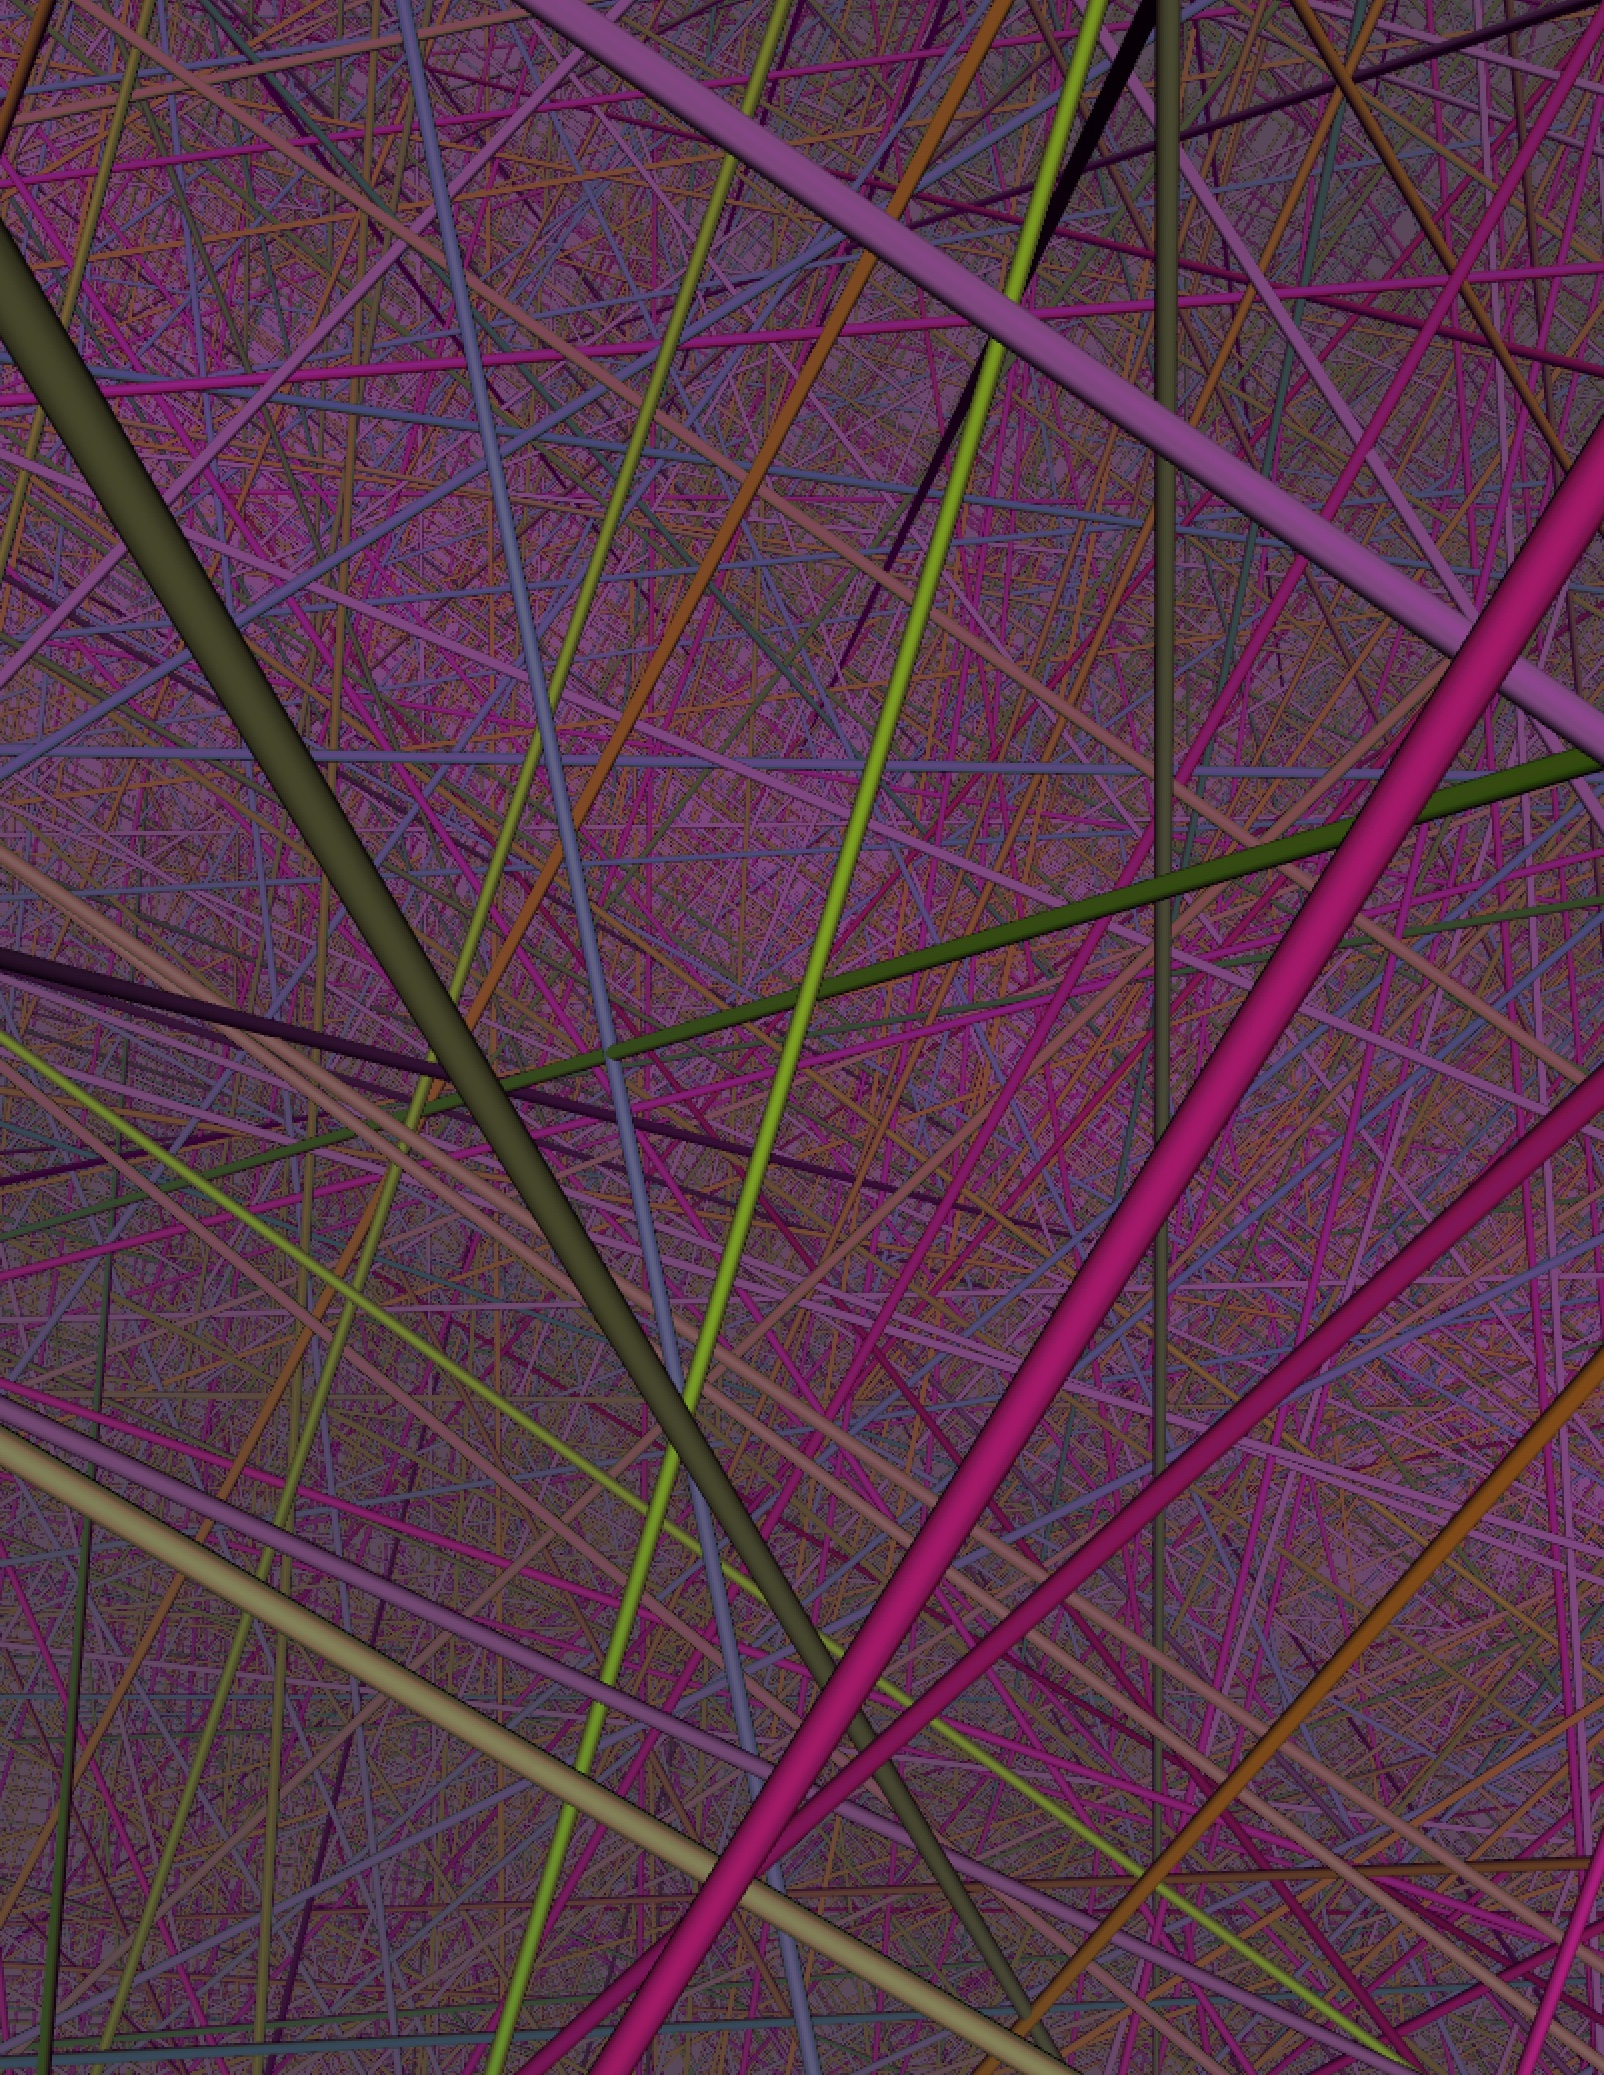
\includegraphics[width=\paperwidth,height=\paperheight]{figures/straight_lines.jpeg}};
 \fill [black, opacity=0.7]
       (\Px,\Py) -- (\Px,\Py+\Ly) -- (\Px+\Lx,\Py+\Ly)-- (\Px+\Lx,\Py) -- cycle;
\node[anchor=north west, align=left, text=white, font=\Huge] at (\Px+4.5,\Py+\Ly-1) { 
Deliverable D1/M1: \\ 
Simulation of Initial Irradiation Damage};
% \node[anchor=north west] at (\Px+4.5,\Py+\Ly-2) {\Huge{\textcolor{white}{
% and its Alloys}}};
\node[anchor=north west] at (\Px+4.5,\Py+\Ly-4) {\Large{\textcolor{white}{
\today}}};
\draw[very thick,orange]  (\Px,\Py+0.5*\Ly) --  (\Px+\Lx,\Py+0.5*\Ly);

\node[anchor=north west] at (\Px+4.5,\Py+\Ly-6) {\Huge{\textcolor{white}{
Multiscale Materials Solutions (MMS)}}};
\node[anchor=north west] at (\Px+4.5,\Py+\Ly-7) {\large{\textcolor{white}{Giacomo Po \& Nasr Ghoniem
}}};
\node[anchor=north west] at (\Px+4.5,\Py+\Ly-8) {\large{\textcolor{white}{
}}};
 \end{tikzpicture}


\newpage
\section*{Contacts}
Multiscale Materials Solutions, LLC\\
Giacomo Po \qquad \emph{Phone: (310) 437-9648}   \\
    \href{mailto:gpo@miami.edu}{gpo@miami.edu} \\
    Nasr Ghoniem \qquad
\emph{Phone: (818) 472-4669}  \\
    \href{mailto:ghoniem@ucla.edu}{ghoniem@ucla.edu} 


\section*{Abstract}

This report documents progress on Deliverable D1, \emph{Multiscale Simulation Methodology}, and, in particular, on Milestone D1/M1, \emph{Simulation of Initial Irradiation Damage}, of the current Statement of Work. The objective of Deliverable D1 is to develop and extend a spatially resolved Cluster Dynamics (CD)–Discrete Dislocation Dynamics (DDD) framework for simulating the nucleation and growth of irradiation-induced defect species in zirconium and its alloys. We summarize the Spatially Resolved Cluster Dynamics (SRCD) model, including its conservation equations, the quasi-static approximation for mobile species, and loop evolution with nucleation. We present a reduced (zero-dimensional) CD model of irradiated zirconium ({\ZrOd}) that specifies the reaction rates under irradiation, the diffusional-anisotropy-difference (DAD) loop bias, the network sink strengths and fluxes, the cascade source partitioning, and the rate equations governing microstructural evolution. The reduced 0D model is calibrated through a formal parameter-identification procedure, in which its kinetic parameters are optimized against the available experimental database for irradiated zirconium by minimizing a normalized objective functional that measures the misfit between predicted and measured microstructural observables, including dislocation-loop number densities, mean loop sizes, and their evolution with dose and temperature. The calibrated model reproduces the observed point-defect kinetics, the loop microstructure, and the evolution of the dislocation network and its associated sink spacing while satisfying defect-conservation checks, thereby establishing quantitative agreement between the 0D CD model and the experimental data across the range of irradiation conditions considered. The calibrated kinetics are then transferred to a fully three-dimensional, spatially resolved CD implementation in {\MoD} ({\ZrM}), solved on a finite-element mesh. Under spatially homogeneous conditions, the 3D model is verified against the ({\ZrOd}) solution, reproducing the mobile-defect concentrations, loop densities, and loop content to within numerical tolerance. Building on this verification, the 3D model generates continuous spatial fields of defect-cluster concentrations, loop populations, and grain-boundary defect profiles as functions of temperature and irradiation dose. These spatially resolved predictions remain fully consistent with the calibrated {\ZrOd} results, and, through them, with the experimental database, while additionally resolving spatial features—such as defect concentration gradients and depletion profiles near grain boundaries—that are inaccessible to the 0D description. Together, these results establish a calibrated and internally consistent multiscale CD capability for predicting the initial irradiation-damage state in zirconium and its alloys.
\newpage
\tableofcontents
\newpage
\section{Introduction}
The first deliverable under the current SOW is Deliverable D1: \emph{Multiscale Simulation Methodology}. The objective is to develop and/or extend a Spatially Resolved Cluster Dynamics (SRCD)–Discrete Dislocation
Dynamics (DDD) framework to simulate the nucleation and growth of irradiation-induced
defect species in Zirconium. The framework shall generate continuous spatial fields describing defect
species concentrations as functions of temperature and irradiation dose. Model parameters shall be
calibrated to capture representative defect species and behaviors observed in Zirconium and its
alloys.
The methodology combines CD simulations to establish the irradiation-induced initial microstructure
with a nucleation criterion for ⟨a⟩ dislocation loops once a threshold damage level (dpa) is reached.

In milestone D1/M1: \emph{Simulation of Initial Irradiation Damage}, spatially resolved CD simulations
shall be used to predict microstructural evolution, including defect nucleation and growth.
Outputs shall consist of continuous spatial fields of defect cluster concentrations at prescribed
temperatures and irradiation doses. Results shall be validated against experimental data across a
range of irradiation conditions.
We report here on our progress in the implementation of deliverable D1, specifically milestone 1 (D1/M1).


\section{Spatially Resolved Cluster Dynamics - The \texttt{ZrMicro-3d} Code}
\label{sec:SRCD}

MoDLib2 implements a SRCD model of  the irradiation defect microstructure, where defect clusters are represented by continuum fields. The method is called ``\textbf{reduced}" because it resolves the concentration of a limited number of \textbf{mobile} defect clusters, each having a fixed defect content Clusters of larger sizes, which are considered to be \textbf{immobile}, have their spatial description limited to their number density and total defect content, without resolving their size distribution explicitly.

\subsection{Mobile defect clusters}
The mobile defect clusters are defined by the \textttclr{mobileSpeciesVector}, a vector parameter set in the material file. For example, \textbf{Zr\_CD4.txt} defines
   \begin{commandshell}
    mobileSpeciesVector=-1 1 2 3;	
    \end{commandshell}
\noindent so that four mobile species are considered: single vacancies, self-interstitials, di-interstitials, and tri-interstitials. We denote this vector $\spvec{m}_M$; its entries are the \emph{signed} cluster sizes $m^k$, with the polarity $p^k=m^k/|m^k|\in\{+1,-1\}$ selecting interstitial ($p=+1$) or vacancy ($p=-1$) character, and $|m^k|$ the number of point defects in the cluster. For the example above $\spvec{m}_M=[-1,+1,+2,+3]^T$ and $\spvec{p}_M=[-1,+1,+1,+1]^T$. As in Section~\ref{sec:immobileClusters}, we use the boolean selectors $\mathcal{M}_i=\tfrac12(1+\spvec{p}_M)$ and $\mathcal{M}_v=\tfrac12(1-\spvec{p}_M)$.


MoDELib2 solves the following steady-state reaction-diffusion partial differential equation (PDE) for the mobile content field $\spvec{c}_M=[c^v,c^i,c^{2i},c^{3i}]^T$, expressed in fractional (per-atom) units:
\begin{align}
\label{Eq:master_c}
    \spvec{0} = - \bm \nabla \cdot
\spvec{J}
+ \spvec{P}_{M}+\tfrac{1}{2}\,(\spmat{I}\otimes\spvec{c}_M^T)\spmat{R}_2\,\spvec{c}_{M}
+ (\spmat{E}-\spmat{D})\,\spvec{c}_{M}+\spvec{S}_{vL}
\end{align}
Throughout this work, we distinguish two kinds of non-scalar quantities by their typeface. Upright sans-serif bold denotes arrays in \emph{species space} (indexed by the mobile defect species $v,i,2i,3i$ or by loop family), with lowercase symbols for vectors, e.g. the concentration array $\spvec{c}_M$, the stacked flux $\spvec{J}$, and the vacancy-loop dissolution source $\spvec{S}_{vL}$ (Eq.~\ref{eq:Semit}), and uppercase symbols for matrices, e.g. the reaction matrix $\spmat{D}$, the emission matrix $\spmat{E}$, and the second-order reaction matrix $\spmat{R}_2$. Bold-italic (e.g. $\bm J^x$, $\bm D^x$, $\bm\nabla$, $\bm\sigma$) is reserved for ordinary vectors and tensors in \emph{Cartesian space}. Thus, the entries $\bm J^x$ of the species-space flux array $\spvec{J}$ are themselves Cartesian vectors, and the divergence $\bm\nabla\cdot$ acts on each entry.

The stacked species flux collects the four Cartesian fluxes of the mobile species,
\begin{align}\label{eq:Jdef}
\spvec{J}=\begin{bmatrix}
 \bm{J}^v \\
 \bm{J}^i \\
 \bm{J}^{2i} \\
 \bm{J}^{3i}
\end{bmatrix}\, ,
\end{align}
and the second-order reaction matrix, whose rows contract the concentration array with the per-species reaction matrices $\spmat{R}_2^x$ of Eq.~\eqref{Eq:R2}, is
\begin{align}\label{eq:R2def}
\spmat{R}_2=\begin{bmatrix}
\spmat{R}_{2}^{v} \\
\spmat{R}_{2}^{i} \\
\spmat{R}_{2}^{2i} \\
\spmat{R}_{2}^{3i}
\end{bmatrix}\, .
\end{align}
In Eq.~\eqref{Eq:master_c} this stacked array enters through the contraction $\tfrac{1}{2}\,(\spmat{I}\otimes\spvec{c}_M^T)\,\spmat{R}_2\,\spvec{c}_{M}$, where $\spmat{I}$ is the $4\times4$ identity and $\otimes$ the Kronecker product; its $x$-th entry is $\tfrac{1}{2}\,\spvec{c}_M^T\spmat{R}_2^{x}\,\spvec{c}_{M}$, so the term is a vector in species space.

Here $\bm J^x =-\bm D^x\bm\nabla c^x$ is the diffusive flux of species $x$, with a possibly-anisotropic diffusion tensor $D^x_{ij}=D^x_{0ij}\exp(-E^{xm}_{ij}/k_BT)$ whose pre-exponential factors $D^x_{0ij}$ and migration energies $E^{xm}_{ij}$ are the material-file vectors \textttclr{mobileSpeciesD0\_SI} and \textttclr{mobileSpeciesEnergyMigration\_eV}. Consistent with Section~\ref{app:A}, the scalar mobility of species $x$ is the jump frequency $\omega_x=z_c\nu_x\exp(-E_x^m/k_BT)$, and the associated point-defect fluxes entering the loop coupling are $\phi_v=\omega_v c^v$ and $\phi_i=\omega_i(c^i+2c^{2i}+3c^{3i})$.

The vector $\spvec{P}_M$ is the cascade production term,
\begin{align}\label{Eq:PGM}
   \spvec{P}_{M} =    G \varepsilon \spvec{f}\,,
\end{align}
where $G$ is the nominal dpa rate (\textttclr{doseRate\_dpaPerSec}), and $\varepsilon$ is the cascade surviving efficiency\\ (\textttclr{mobileSpeciesSurvivingEfficiency}), and $\spvec{f}$ the fraction vector partitioning cascade production among the mobile clusters. Expanded component-wise, and accounting for the per-cluster entry of the di- and tri-interstitial sources ($G_{2i}/2$ and $G_{3i}/3$), $\spvec{P}_M$ reproduces the $0$D cascade sources $\{G_v,\,G_i,\,\tfrac12 G_{2i},\,\tfrac13 G_{3i}\}$ of Section~\ref{app:A}, with $G_x=G\varepsilon_x$ the corresponding partition of the displacement rate.

The $\spmat{R}_2$-term represents second-order reactions between mobile species, modeling the collision of two mobile species to form a third species. For the chosen vector of mobile species, we have
\begin{align}\label{Eq:R2} 
    {\spmat{R}}^{v}_{2} = -
\begin{bmatrix} 
0 & \beta^{v,i} & \beta^{v,2i} & \beta^{v,3i} \\ 
\beta^{v,i}  & 0 & 0 & 0 \\
\beta^{v,2i} & 0  & 0 & 0 \\
\beta^{v,3i} & 0 & 0 & 0
\end{bmatrix}\,, &&
%
    {\spmat{R}}^i_2 = -
\begin{bmatrix} 
0 & \beta^{v,i}  & -\beta^{v,2i} & 0 \\ 
\beta^{v,i}  & 2\beta^{i,i} & \beta^{i,2i} & {\beta^{i,3i}} \\
-\beta^{v,2i} & \beta^{i,2i}  & 0 & 0 \\
0 & {\beta^{i,3i}} & 0 & 0
\end{bmatrix}\,, \nonumber \\ 
%
%
    {\spmat{R}}^{2i}_{2} = -{2}
\begin{bmatrix} 
0 & 0  & \beta^{v,2i} & -\beta^{v,3i}  \\ 
0  & -\beta^{i,i} & \beta^{i,2i} & 0 \\
\beta^{v,2i} & \beta^{i,2i}  & {2\beta^{2i,2i}} & {\beta^{2i,3i}} \\
-\beta^{v,3i}  & 0 & {\beta^{2i,3i}} & 0
\end{bmatrix}\,,  &&
%
%
    {\spmat{R}}^{3i}_{2} = -{3}
\begin{bmatrix} 
0 & 0  & 0 & \beta^{v,3i}  \\ 
0  & 0 & -\beta^{i,2i} & {\beta^{i,3i}} \\
0 & -\beta^{i,2i}  & 0 & {\beta^{2i,3i}} \\
\beta^{v,3i}  & {\beta^{i,3i}} & {\beta^{2i,3i}} & {2\beta^{3i,3i}}
\end{bmatrix} \,,
\end{align}
where $\beta^{m,n}$ in Eq.~\eqref{Eq:R2} represents the reaction rates between species $m$ and $n$. 
A positive reaction rate  indicates  production, while the negative sign means its consumption. The reaction rates are given by the equation
\begin{align}
    \beta^{m,n} = \frac{A^{m,n}}{\Omega {|\mathcal{M}_m \mathcal{M}_n|}} (\overline{D}^{m} + \overline{D}^{n})  (r^{m} + r^{n}) \,,
\end{align}
The pairwise rate constants use the sum of the two reactant jump frequencies, consistently with the $0$D reaction rates $R_{a,b}=(\omega_a+\omega_b)C_aC_b$ of Section~\ref{app:A},
\begin{align}\label{eq:beta}
\beta^{m,n}=(\omega_m+\omega_n)\, ,
\end{align}
with the recombination-volume factor $\beta_r$ carried on the interstitial--vacancy channel ($\beta^{v,i}\to\beta_r(\omega_i+\omega_v)$) and the combinatorial factors $2$ and $4$ retained on the like-species reactions ($R_{i,i}=2\omega_iC_i^2$, $R_{2i,2i}=4\omega_{2i}C_{2i}^2$). The capture radius $r^m$ used to build $\beta^{m,n}$ follows the point-defect / prismatic-loop geometry
\begin{equation}
    r^m =
    \begin{cases}
        \displaystyle
        \left(\frac{3\Omega_0}{4\pi}\right)^{1/3},
        & \left|m^m\right|=1,
        \\[10pt]
        \displaystyle
        \left(\frac{\left|m^m\right|\Omega_0}{\pi b}\right)^{1/2},
        & \left|m^m\right|>1.
    \end{cases}
    \label{eq:mobile_capture_radius}
\end{equation}
Expanding $\tfrac12\,\spvec{c}_M^T\spmat{R}_2^{x}\spvec{c}_M$ component-wise reproduces the $0$D pair-reaction budget of each monomer/small-cluster equation, e.g. the interstitial line yields $R_{2i,v}+2\mathcal{E}_{2i}+3\mathcal{E}_{3i}-(R_{i,v}+R_{i,i}+R_{i,2i}+R_{i,3i})$ once the emission and sink terms below are added.

The $\spmat{E}$-term represents the thermal dissociation (emission) of mobile species. It is the matrix
\begin{align}\label{Eq:R1}
   {\spmat{E}} =  -
\begin{bmatrix}
 0 & 0 & 0 & 0 \\ 
0 & 0 & -\alpha^{i,2i} & -\tfrac{1}{3}\alpha^{i,3i}\\ 
0 & 0 & \alpha^{i,2i} & -\tfrac{2}{3}\alpha^{i,3i} \\ 
0 & 0 & 0 &    \alpha^{i,3i}
\end{bmatrix}\, ,
\end{align}
where $\alpha^{x,nx}$ is the dissociation rate of an $nx$-cluster emitting a point defect of type $x$,
\begin{align}
    \alpha^{m,n} = \beta^{m,n} \exp{ \left( -\frac{E^b_{m,n}}{k_B T} \right)}\, ,\label{eq:alpha}
\end{align}
With $E^b_{m,n}$, the binding energy of the $(m+n)$-size cluster (\textttclr{mobileSpeciesBindingEnergy\_eV}). Component-wise, $\spmat{E}\spvec{c}_M$ reproduces the $0$D thermal-emission terms $\mathcal{E}_{2i}=\omega_{2i}e_{2i}C_{2i}$ and $\mathcal{E}_{3i}=\omega_{3i}e_{3i}C_{3i}$ of Section~\ref{app:A}.

The $\spmat{D}$-term is the linear reaction matrix that governs the annihilation of mobile defects at immobile sinks. It absorbs the mobile diffusivities into the sink strengths, which themselves combine the network sinks with the mass-conserving loop absorption. The mobile-to-immobile reaction matrix is:
\begin{equation}\label{eq:KM}
\spmat{D}=\mathrm{diag}\{\spvec{\omega}\odot\spvec{C}_s\}+\spmat{D}_d\,\spmat{K}_{\mathcal L},\qquad
\spmat{D}_d=\mathrm{diag}\{\overline{D}^v,\overline{D}^i,\overline{D}^{2i},\overline{D}^{3i}\} 
\end{equation}
where $\spvec{C}_s=[C_s^v,C_s^i,C_s^i,C_s^i]^T$ are the network-only sink concentrations of Section~\ref{app:A} ($C_s^v=\tfrac{a^2}{z_c}\rho_N$, $C_s^i=\tfrac{a^2}{z_c}Z_N\rho_N$) and $\spvec{\omega}=[\omega_v,\omega_i,\omega_i,\omega_i]^T$. The first term reproduces the network sink reactions $R_{x,s}=\omega_x C_x C_s^x$, while $\spmat{K}_{\mathcal L}$ carries the loop-absorption debits $\text{loop\_abs}_i,\text{loop\_abs}_v$ defined in Eq.~\eqref{eq:loopcoupling}, so that mobile losses to loops match exactly the content gained by the immobile families and no defect is double-counted. The network term is already a reaction rate, whereas the loop sink strengths acquire the mobile diffusivities, so both contributions have units of frequency (Hz), and $\overline{D}^m$ is the (orientationally averaged) diffusion coefficient of mobile species $m$.

The loop sink-strength block $\spmat{K}_{\mathcal L}$ is diagonal in the mobile species and collects, for each mobile defect $m$, the total sink strength of the immobile loop families,
\begin{align}\label{eq:KL_matrix}
\spmat{K}_{\mathcal L}=\mathrm{diag}\{\spvec{k}^2\},\qquad
\spvec{k}^2=\begin{bmatrix} k_v^2 \\ k_i^2 \\ k_{2i}^2 \\ k_{3i}^2 \end{bmatrix},\qquad
k_m^2=\sum_{I\mathcal{L}}\left\langle k^2_{I\mathcal{L},m}\right\rangle,
\end{align}
where the sum runs over the immobile families $I\mathcal{L}\in\{c\mathcal{L},a\mathcal{L},bp\}$ and each partial sink strength is
\begin{align}\label{eq:partial_sink}
\left\langle k^2_{a\mathcal{L},m }\right\rangle &= Z_{a\mathcal{L},tot}^m\, 2\pi r^{a\mathcal{L}} n^{a\mathcal{L}}, \\
\left\langle k^2_{c\mathcal{L},m }\right\rangle &= Z_{c\mathcal{L},tot}^m\, 2\pi r^{c\mathcal{L}} n^{c\mathcal{L}}, \\
\left\langle k^2_{bp,m }\right\rangle &= \alpha_{bp} s_{bp} \pi r_{bp} n_{bp},
\end{align}
with $Z_{I\mathcal{L},tot}^m$ the corresponding bias factors, $r^{I\mathcal{L}}$ the family radii, and $n^{I\mathcal{L}}$ the family densities. The per-family bias factors $Z^m_{a_1\mathcal L},Z^m_{a_2\mathcal L},Z^m_{a_3\mathcal L}$ and $Z^m_{vL}$ entering the partial sink strengths are exactly the orientation- and species-resolved capture efficiencies of Eqs.~\eqref{eq:Za1}--\eqref{eq:Za3} and Eq.~\eqref{eq:ZvL}, so that both the loop growth and the mobile-defect sinks are built from a single set of bias factors. Beyond the stress-induced anisotropy (SIPA) carried by these factors, the intrinsic diffusional anisotropy of defects in the non-cubic (h.c.p.) lattice also modifies the absorption efficiency. This diffusion-anisotropy-difference (DAD) effect is characterized by $Z^{\mathrm{DAD},0}_{\mathcal L,m}$, which yields
\begin{align}\label{eq:DAD0}
Z^{\mathrm{DAD},0}_{a\mathcal L,m} = Z^0_m\left(\frac{p^m+(p^m)^{-2}}{2}\right),\qquad
Z^{\mathrm{DAD},0}_{c\mathcal L,m} = Z^0_m\, p^m,
\end{align}
with $p^m=(D_c^m/D_a^m)^{1/6}$ a parameter characterizing the diffusional anisotropy of species $m$, and $Z^0_m$ its bias factor for an isotropically diffusing defect without stress. Unlike traditional cluster-dynamics models, which presume a fixed bias factor for DAD, the present spatially-resolved formulation incorporates the DAD effect naturally through the tensorial description of the mobile-species flux.

At zero stress, the partial sink strengths of the prismatic ($a$-type) and basal ($c$-type) loops simplify to
\begin{align}
\left\langle k^2_{a\mathcal{L},m }\right\rangle &= Z^0_{m}\left( p^m + (p^m)^{-2} \right)\pi r^{a\mathcal{L}} n^{a\mathcal{L}} \label{Eq:asink_strength_simple}\\
\left\langle k^2_{c\mathcal{L},m }\right\rangle &= Z^0_{m}\, p^m\, 2\pi r^{c\mathcal{L}} n^{c\mathcal{L}} \label{Eq:csink_strength_simple}
\end{align}
For isotropically diffusing defects (single vacancies and single interstitials, $p=1$), these expressions recover the traditional dislocation sink strength, whereas for di- and tri-interstitials on the prismatic plane, $p<1$ gives $\left\langle k^2_{c\mathcal{L},m }\right\rangle < \left\langle k^2_{a\mathcal{L},m }\right\rangle$. The sink strength of vacancy clusters is interpolated from the bi-pyramid value $\left\langle k^2_{bp,m }\right\rangle$ toward the basal-loop value $\left\langle k^2_{c\mathcal{L},m }\right\rangle$ as the reconstructed vacancy loops flatten onto the basal plane.



The mobile species PDE~\eqref{Eq:master_c} is accompanied by the concentration boundary condition\footnote{
Eq.~\eqref{mobileBC} is a pure essential (Dirichlet) BC representing a perfect sink. A more general Robin-type BC
\begin{align}
-\bm J^k\cdot \bm n = h^k\left[c^k(\bm x)-c^k_\text{bnd,eq}(\bm x)\right]\, ,
\end{align}
recovers the perfect sink condition as $h^k\rightarrow\infty$ and the no-flux condition as $h^k\rightarrow0$.
}
(BC)
\begin{align}
\spvec{c}_M(\bm x)=\spvec{c}_\text{bnd,eq}(\bm x) && \text{(mobile species BC)}\, ,
\label{mobileBC}
\end{align}
where $c^k_\text{bnd,eq}(\bm x)$ is the local concentration of the species in equilibrium with the boundary,
\begin{align}
c^k_\text{bnd,eq}(\bm x)=c^k_0(\bm x)\exp\left(-\frac{m^k\,t_n(\bm x)\Omega}{k_BT}\right) \, ,
\label{Eq:mobileBC}
\end{align}
in which $t_n$ is the normal traction on the boundary and $c^k_0(\bm x)$ is the thermal-equilibrium concentration
\begin{align}
c^k_0(\bm x)= |m^k|\exp\left(-\frac{E^f_k+m^k\,q\,\Omega_k^r}{k_BT}\right)\, ,
\label{Eq:mobileC0}
\end{align}
where $q(\bm x)=-\text{tr}(\bm\sigma(\bm x))/3$ is the local pressure, $\Omega_k^r=\omega_k^r\Omega$ the relaxation volume of the $k$-th cluster (with a relative relaxation volume $\omega_k^r$, \textttclr{mobileSpeciesRelRelaxVol}), and $E_k^f$ its boundary formation energy (\textttclr{mobileSpeciesEnergyFormation\_eV}). The stress terms in Eqs.~\eqref{Eq:mobileBC} and~\eqref{Eq:mobileC0} are multiplied by the signed cluster size $m^k$, rendering opposite effects for interstitial and vacancy-type clusters.


\subsection{Immobile defect clusters}
\label{sec:immobileClusters}

In the CD implementation of MoDELib2, interstitial clusters larger than $m_\text{max}$ and vacancy clusters larger than $m_\text{min}$ are considered immobile and are treated as dislocation loops. In irradiated Zr four immobile loop families are represented, following Section~\ref{app:A}: one vacancy ($\langle c\rangle$) loop family and three interstitial ($\langle a\rangle$) loop families indexed by the orientation of their Burgers vector along the three prismatic directions $a_1,a_2,a_3$,
\begin{align}
\mathcal{L}=\{vL,\ ia_1,\ ia_2,\ ia_3\}\, ,
\end{align}
Each family $k$ carries a polarity $p^k\in\{+1,-1\}$ ($p=+1$ interstitial, $p=-1$ vacancy),
\begin{align}
p^{vL}=-1\, ,\qquad p^{ia_1}=p^{ia_2}=p^{ia_3}=+1\, ,
\end{align}
so that the interstitial and vacancy families are selected by the boolean vectors $\mathcal{I}_i=\tfrac12(1+p)$ and $\mathcal{I}_v=\tfrac12(1-p)$.

Each immobile family is described by two spatially--resolved fields: the \emph{cluster density} $n^k$, i.e. the number of loops of family $k$ per host atom, and the \emph{defect content} $c^k$, i.e. the number of point defects stored in that family per host atom,
\begin{align}
\spvec{n}_I(\bm x)&=\left[n^{vL},n^{ia_1},n^{ia_2},n^{ia_3}\right]^T & \text{(cluster density, clusters per atom)}\\
\spvec{c}_I(\bm x)&=\left[c^{vL},c^{ia_1},c^{ia_2},c^{ia_3}\right]^T & \text{(defect content, defects per atom).}
\end{align}
Both are dimensionless (fractional) quantities. The mean number of point defects per cluster of family $k$ follows from the ratio of content to density,
\begin{align}\label{eq:mI}
m^k=\frac{c^k}{n^k}\, ,
\end{align}
and the mean loop radius is recovered from the content--to--density ratio through the loop length scales $\ell_a,\ell_c$ of Section~\ref{app:A},
\begin{align}\label{eq:rI}
r^k=\ell^k\sqrt{\frac{c^k}{n^k}}\, ,\qquad \ell^{vL}=\ell_c\, ,\quad \ell^{ia_1}=\ell^{ia_2}=\ell^{ia_3}=\ell_a\, ,
\end{align}
which, expanded family by family, reproduces the $0$D content relations $r_{vL}=\ell_c\sqrt{C_{vL}^{v}/C_{vL}}$, $r_{ia_1}=\ell_a\sqrt{C_{ia_1}^{i}/C_{ia_1}}$ of Eq.~(\ref{eq:DAD})'s companion set, with the identification $n^k\leftrightarrow C_{XL}$ and $c^k\leftrightarrow C_{XL}^{x}$.

The shape of a cluster depends on its size $m^k$: it has been shown that vacancy clusters transition from a compact bi-pyramid geometry to a planar (platelet) loop with increasing cluster size. We therefore include this transition of clusters from volumetric defects to planar loops, so that the effective radius of family $k$ interpolates between the two limiting geometries,
\begin{align}\label{eq:Rtransition}
R^k(m^k)=\left[1-S^k(m^k)\right]R_{\mathrm{pyr}}^k+S^k(m^k)R_{\mathrm{loop}}^k\, ,
\end{align}
where the pyramid and loop radii are
\begin{align}\label{eq:Rpyrloop}
R_{\mathrm{pyr}}^k=\left(\frac{m^k\Omega_0}{\sqrt{8}}\right)^{1/3}\, ,\qquad R_{\mathrm{loop}}^k=\sqrt{\frac{m^k\Omega_0}{\pi b^k}}\, .
\end{align}
The function $S^k$ is a sigmoidal transition function operating a smooth switch between the two shapes,
\begin{align}\label{eq:Ssigmoid}
S^k(m^k)=\frac{1}{1+\exp\left[-\dfrac{m^k-m_0^k}{w^k}\right]}\, ,
\end{align}
whose midpoint and steepness are set by
\begin{align}\label{eq:Sparams}
m_0^k=\frac{m_{\min}^k+m_{\max}^k}{2}-m_s^k\, ,\qquad w^k=w_0\left(m_{\max}^k-m_{\min}^k\right)\, ,
\end{align}
so that clusters with $m^k\lesssim m_{\min}^k$ are predominantly bi-pyramid-like while clusters with $m^k\gtrsim m_{\max}^k$ are predominantly loop-like. The same sigmoidal function interpolates the cluster formation-volume tensor,
\begin{align}\label{eq:Omegatransition}
\bm\Omega^k(m^k)=\left(1-S^k(m^k)\right)\bm\Omega^k_{\mathrm{pyr}}+S^k(m^k)\bm\Omega^k_{\mathrm{loop}}\, ,
\end{align}
with the loop and pyramid limits
\begin{align}\label{eq:Omegalimits}
\bm\Omega^k_{\mathrm{loop}}=\mathcal{I}^k\,\frac{\bm b^k\otimes\bm b^k}{\bm b^k\cdot\bm b^k}\,V^k\, ,\qquad \bm\Omega^k_{\mathrm{pyr}}=\mathcal{I}^k\,\frac{\mathbb{I}}{3}\,V^k\, ,
\end{align}
where $V^k=m^k\Omega_0$ is the cluster volume and $\mathcal{I}^k$ the loop selector. The pyramid regime applies to the sub-critical vacancy ($\langle c\rangle$) family, which collapses smoothly onto the planar vacancy loop as it grows.

Both fields obey spatially--resolved ordinary differential equations coupled to the mobile PDE~\eqref{Eq:master_c}: a \emph{density} equation for $\spvec{n}_I$ (nucleation and annealing of loops) and a \emph{content} equation for $\spvec{c}_I$ (defect storage through absorption).  These are developed in turn below.



The loop density evolves by nucleation and thermal annealing,
\begin{align}\label{eq:cIode}
\frac{d\spvec{n}_I}{dt}=\dot{\spvec{N}}^{\mathrm{nuc}}-\spvec{a}_n-\Delta\spvec{N}\, ,
\end{align}
where $\dot{\spvec{N}}^{\mathrm{nuc}}$ is the nucleation-rate vector, $\spvec{a}_n$ the (vacancy-loop) annealing vector, and $\Delta\spvec{N}$ the coalescence sink. The coalescence sink is diagonal in the loop family and, for each family $k\in\{vL,a_1L,a_2L,a_3L\}$, reproduces the two-channel geometric coalescence of Section~\ref{sec:coal} (a like-loop channel that conserves content and a loop--network channel that is booked as network absorption),
\begin{align}\label{eq:DeltaN}
\Delta\spvec{N}=\begin{bmatrix}\Delta N^{vL}\\[2pt]\Delta N^{a_1L}\\[2pt]\Delta N^{a_2L}\\[2pt]\Delta N^{a_3L}\end{bmatrix},\qquad
\Delta N^{k}=\bigl(\nu_{LL}^{k}\,\phi_{LL}^{k}+\nu_{LN}^{k}\,\phi_{LN}^{k}\bigr)\,n^{k},
\end{align}
with the Avrami overlap probabilities $\phi_{LL}^{k},\phi_{LN}^{k}$ and rate scales $\nu_{LL}^{k},\nu_{LN}^{k}$ of the coalescence model of Section~\ref{sec:coal}, and $n^{k}$ the family density. The two terms are exactly the $0$D like-loop and loop--network number-loss rates $\Delta N=\nu_{LL}\phi_{LL}\,n+\Delta N_{LN}$ with the $0$D number concentration replaced family by family by $n^{k}$. Interstitial loops nucleate from homogeneous clustering of mobile species plus a cascade seed, while vacancy loops nucleate from the cascade only,
\begin{align}\label{eq:Nnuc}
\dot{\spvec{N}}^{\mathrm{nuc}}=
\spvec{w}(\bm\sigma)\,\Phi_{\mathrm{clus}}+\spvec{G}_{\mathcal{L}}\oslash\spvec{n}^{\mathrm{nuc}}\, ,
\end{align}
with $\Phi_{\mathrm{clus}}=R_{i,3i}+R_{2i,2i}$ the interstitial-clustering flux, the stress-dependent orientation weight vector $\spvec{w}(\bm\sigma)=[\,0,\,w_{a_1}(\bm\sigma),\,w_{a_2}(\bm\sigma),\,w_{a_3}(\bm\sigma)]^T$, the cascade-loop source vector $\spvec{G}_{\mathcal{L}}=[\,G_{vL},G_{ia_1},G_{ia_2},G_{ia_3}]^T$, per-loop seed sizes $\spvec{n}^{\mathrm{nuc}}=[\,n_{vL}^{\mathrm{nuc}},n_{ia}^{\mathrm{nuc}},n_{ia}^{\mathrm{nuc}},n_{ia}^{\mathrm{nuc}}]^T$, and $\oslash$ the elementwise (Hadamard) division. Expanding \eqref{eq:Nnuc} component-wise recovers exactly the $0$D nucleation rates $\dot N_{ia_1}^{\mathrm{nuc}}=w_{a_1}(\bm\sigma)(R_{i,3i}+R_{2i,2i})+G_{ia_1}/n_{ia}^{\mathrm{nuc}}$, and likewise for $ia_2,ia_3,vL$. The orientation weights $w_{a_k}(\bm\sigma)=\tfrac13(1+\chi\,\hat\sigma_{kk})$, with $\sum_k w_{a_k}=1$, bias the cascade nucleation seed among the three prismatic directions through the resolved stress $\sigma_{kk}=\hat{\bm b}_k\cdot\bm\sigma\cdot\hat{\bm b}_k$ projected onto each Burgers orientation $\hat{\bm b}_k$ ($k=a_1,a_2,a_3$) as in Section~\ref{app:A}; at zero stress they reduce to the common seed $\tfrac13$. These linearized weights are the small-stress limit of the stress-induced preferential nucleation (SIPN) partition, in which the cascade-produced defects are distributed among the immobile families through a Boltzmann factor coupling the applied stress $\bm\sigma$ to each family's formation-volume tensor $\bm\Omega^k$,
\begin{align}\label{eq:SIPN}
\chi^k_i=\frac{\exp\left(\dfrac{\bm\sigma:\bm\Omega^k}{k_BT}\right)\mathcal{I}_i^k}{\sum_p\exp\left(\dfrac{\bm\sigma:\bm\Omega^p}{k_BT}\right)\mathcal{I}_i^p}\, ,\qquad \chi^k_v=\frac{\exp\left(\dfrac{\bm\sigma:\bm\Omega^k}{k_BT}\right)\mathcal{I}_v^k}{\sum_p\exp\left(\dfrac{\bm\sigma:\bm\Omega^p}{k_BT}\right)\mathcal{I}_v^p}\, ,
\end{align}
where $\mathcal{I}_i^k$ and $\mathcal{I}_v^k$ are the interstitial and vacancy selectors, and the sums run over all immobile families $p$. At zero stress every $\bm\sigma:\bm\Omega^k$ vanishes and the interstitial partition reduces to the common seed $\tfrac13$ among the three prismatic orientations, recovering $w_{a_k}(\spvec{0})=\tfrac13$. The annealing vector acts only on the vacancy families,
\begin{align}
\spvec{a}_n=\left[\,\frac{n^{vL}}{\tau_{vL}},\,0,\,0,\,0\right]^T\, ,
\end{align}
with the Arrhenius lifetimes $\tau_{vL}(T)=\tau_{vL}^{0}\exp(E_a^{vL}/k_BT)$.



The defect content of the loops evolves through mass-conserving absorption of mobile defects, cascade deposition, nucleation seeding, and coalescence,
\begin{align}\label{eq:CIode}
\frac{d\spvec{c}_I}{dt}=
\dot{\spvec{G}}^{c}
+\spvec{P}_G
+\spvec{s}^{\mathrm{nuc}}
-\spvec{A}_c
-\Delta\spvec{C}\, .
\end{align}
The coalescence content sink removes stored content only through the loop--network channel (the like-loop channel merges two loops without losing content), so, family by family,
\begin{align}\label{eq:DeltaC}
\Delta\spvec{C}=\begin{bmatrix}\Delta C^{vL}\\[2pt]\Delta C^{a_1L}\\[2pt]\Delta C^{a_2L}\\[2pt]\Delta C^{a_3L}\end{bmatrix},\qquad
\Delta C^{k}=\nu_{LN}^{k}\,\phi_{LN}^{k}\,c^{k},
\end{align}
with $c^{k}$ the family content, matching the $0$D content-loss rate $\Delta C=\nu_{LN}\phi_{LN}\,c$ of Section~\ref{app:A} with the $0$D content replaced family by family by $c^{k}$.
The net content-growth vector $\dot{\spvec{G}}^{c}$ collects, for each family, the absorption of its own defect type minus absorption of the opposite type (a defect--loop recombination). The mobile point-defect fluxes are the vacancy flux $\phi_v$ and the interstitial flux $\phi_i$,
\begin{align}\label{eq:fluxdef}
\phi_v=\omega_v\,c^v\, ,\qquad
\phi_i=\omega_i\left(c^i+2\,c^{2i}+3\,c^{3i}\right)\, ,
\end{align}
from Section~\ref{app:A}. Each immobile family grows by capturing its like defect and shrinks by capturing the opposite defect: the vacancy loop $vL$ captures $\phi_v$ and recombines with $\phi_i$, whereas the three prismatic interstitial loops $a_1L$, $a_2L$ and $a_3L$ capture $\phi_i$ and recombine with $\phi_v$. With the geometric capture prefactor $\pi_k=(\ell_c/\ell)\sqrt{c^k n^k}$ of family $k$ (with the $c$-loop efficiency $Q$ folded into $\pi_{vL}$) and the orientation-resolved capture efficiencies $Z^k$, the absorption prefactors and the diffusional-anisotropy-difference (DAD) bias give the content-growth rate of each family,
\begin{align}\label{eq:loopcoupling}
\dot G^{c}_{vL}   &=p_{vL}\,\pi_{vL}\left(Z^{vL}_{v}\,\phi_v-Z^{vL}_{i}\,\phi_i\,g(r_{vL})\right)\, ,\\
\dot G^{c}_{a_1L} &=p_{a_1L}\,\pi_{a_1L}\left(Z^{a_1L}_{i}\,\phi_i-Z^{a_1L}_{v}\,\phi_v\right)\, ,\\
\dot G^{c}_{a_2L} &=p_{a_2L}\,\pi_{a_2L}\left(Z^{a_2L}_{i}\,\phi_i-Z^{a_2L}_{v}\,\phi_v\right)\, ,\\
\dot G^{c}_{a_3L} &=p_{a_3L}\,\pi_{a_3L}\left(Z^{a_3L}_{i}\,\phi_i-Z^{a_3L}_{v}\,\phi_v\right)\, ,
\end{align}
where $p_k$ is the defect sign of family $k$ ($p=-1$ for the vacancy loop, $p=+1$ for the interstitial loops) and the minimum-stable-size gate $g(r_{vL})$ acts only on the vacancy-loop channel. Each interstitial loop $a_kL$ sees the DAD bias evaluated at its own resolved stress $\sigma_{kk}=\hat{\bm b}_k\cdot\bm\sigma\cdot\hat{\bm b}_k$, while the vacancy loop carries the basal ($c$-type) bias, so that the orientation-resolved capture efficiencies are
\begin{align}Z^{a_1L}_m(\bm\sigma)&=Z^{\mathrm{DAD},0}_{a,m}\left(1+\frac{\Delta Z^{\mathrm{SIPA}}_{a,m}(\sigma_{11})}{Z^{\mathrm{DAD},0}_{a,m}}\right)\, ,\label{eq:Za1}\\
Z^{a_2L}_m(\bm\sigma)&=Z^{\mathrm{DAD},0}_{a,m}\left(1+\frac{\Delta Z^{\mathrm{SIPA}}_{a,m}(\sigma_{22})}{Z^{\mathrm{DAD},0}_{a,m}}\right)\, ,\label{eq:Za2}\\
Z^{a_3L}_m(\bm\sigma)&=Z^{\mathrm{DAD},0}_{a,m}\left(1+\frac{\Delta Z^{\mathrm{SIPA}}_{a,m}(\sigma_{33})}{Z^{\mathrm{DAD},0}_{a,m}}\right)\, ,\label{eq:Za3}\\
Z^{vL}_m(\bm\sigma)&=Z^{\mathrm{DAD},0}_{c,m}\left(1+\frac{\Delta Z^{\mathrm{SIPA}}_{c,m}(\bm\sigma)}{Z^{\mathrm{DAD},0}_{c,m}}\right)\, ,\label{eq:ZvL}
\end{align}
which all reduce to their stress-free DAD values $Z^{\mathrm{DAD},0}_{a,m}$ (interstitial loops) and $Z^{\mathrm{DAD},0}_{c,m}$ (vacancy loop) when $\bm\sigma=0$. Collecting the four families in the vacancy-first order $\mathcal L=\{vL,a_1L,a_2L,a_3L\}$, the content-growth vector is
\begin{align}\label{eq:Gcarray}
\dot{\spvec{G}}^{c}=
\begin{bmatrix}
\dot G^{c}_{vL}\\[3pt]
\dot G^{c}_{a_1L}\\[3pt]
\dot G^{c}_{a_2L}\\[3pt]
\dot G^{c}_{a_3L}
\end{bmatrix}
=
\begin{bmatrix}
p_{vL}\,\pi_{vL}\left(Z^{vL}_{v}\,\phi_v-Z^{vL}_{i}\,\phi_i\,g(r_{vL})\right)\\[3pt]
p_{a_1L}\,\pi_{a_1L}\left(Z^{a_1L}_{i}\,\phi_i-Z^{a_1L}_{v}\,\phi_v\right)\\[3pt]
p_{a_2L}\,\pi_{a_2L}\left(Z^{a_2L}_{i}\,\phi_i-Z^{a_2L}_{v}\,\phi_v\right)\\[3pt]
p_{a_3L}\,\pi_{a_3L}\left(Z^{a_3L}_{i}\,\phi_i-Z^{a_3L}_{v}\,\phi_v\right)
\end{bmatrix}\, .
\end{align}

The cascade deposition vector $\spvec{P}_G$ delivers the loop-borne fraction of the collision cascade,
\begin{align}\label{eq:PG}
\spvec{P}_G=\spvec{G}_{\mathcal{L}}=G\big(\varepsilon_{ia}\spvec{w}(\bm\sigma)+\varepsilon_{vL}\spvec{w}'\big)\, ,
\end{align}
with $\spvec{w}(\bm\sigma)=[0,w_{a_1},w_{a_2},w_{a_3}]^T$ and $\spvec{w}'=[1,0,0,0]^T$, so that the stress-biased partition among the three interstitial orientations and the vacancy loop is preserved. The nucleation-seeding vector deposits the interstitial atoms consumed by the clustering reactions as newborn loop content,
\begin{align}
\spvec{s}^{\mathrm{nuc}}=\mathcal{N}_c\,[\,0,\,w_{a_1},\,w_{a_2},\,w_{a_3}\,]^T\, ,\qquad
\mathcal{N}_c=4R_{i,3i}+2R_{2i,2i}+3R_{2i,3i}\, ,
\end{align}
and the content-annealing vector returns the birth content of dissolving vacancy embryos to the free pool,
\begin{align}
\spvec{A}_c=\left[\,\frac{c^{vL}}{\tau_{vL}},\,0,\,0,\,0\right]^T\, .
\end{align}

The lifetime $\tau_{vL}$ above is the size-independent survival lifetime of the sub-critical vacancy embryos produced in the cascade, so that $\spvec{a}_n$ and $\spvec{A}_c$ describe the \emph{dissolution} of embryos that fail to reach the minimum stable size; the minimum-stable-size gate $g(r^{vL})$ of \eqref{eq:loopcoupling} confines these terms to the sub-critical population. Vacancy loops that survive and grow lose vacancies through a second, distinct channel: the \emph{thermal emission} of single vacancies from a stable loop, governed by the size-dependent vacancy binding energy. Because the reduced model tracks only the family density $n^{k}$ and content $c^{k}$, the emission rate is evaluated at the mean loop size
\begin{align}\label{eq:meanloopsize}
\bar m^{k}=\frac{c^{k}}{n^{k}}\, ,
\end{align}
and, following the detailed-balance form of \eqref{eq:beta}--\eqref{Eq:R1}, the per-defect thermal-emission rate of the vacancy loop is
\begin{align}\label{eq:loopemission}
\alpha^{v,k}(\bar m^{k})=\beta_{v,k}\,\exp\!\left(-\frac{E_b^{v,k}(\bar m^{k})}{k_BT}\right)\, ,\qquad k=vL\, ,
\end{align}
where $E_b^{v,k}(\bar m^{k})$ is the vacancy binding energy of the mean-size loop, which grows toward its bulk limit with $\bar m^{k}$ so that larger loops emit ever more weakly. This channel reduces the loop content without removing loops, and hence enters the content ODE~\eqref{eq:CIode} through the thermal-emission vector
\begin{align}\label{eq:Aemit}
\spvec{A}_c^{\mathrm{emit}}=\left[\,\alpha^{v,vL}(\bar m^{vL})\,c^{vL},\,0,\,0,\,0\right]^T\, ,
\end{align}
which is subtracted alongside $\spvec{A}_c$ while leaving the density ODE unchanged.

The vacancies released by \emph{both} channels are returned to the free vacancy pool, sourcing the mobile species PDE~\eqref{Eq:master_c} through
\begin{align}\label{eq:Semit}
\spvec{S}_{vL}=\left[\,\frac{c^{vL}}{\tau_{vL}}+\alpha^{v,vL}(\bar m^{vL})\,c^{vL},\ 0,\ 0,\ 0\right]^T\, ,
\end{align}
whose single non-zero entry feeds the mobile vacancy line. By construction $\spvec{S}_{vL}$ is term-by-term identical to the vacancy content removed from the loops by $\spvec{A}_c+\spvec{A}_c^{\mathrm{emit}}$, so the exchange is a pure transfer: every vacancy debited from the immobile families is credited to the mobile pool exactly once, and the total point-defect content is conserved. This transfer is independent of the mass-conserving absorption coupling $\dot{\spvec{G}}^{c}$, so a surviving loop may simultaneously grow by absorbing the excess vacancy flux (debited from $\spvec{c}_M$ via $\spmat{D}$) and shrink by thermal emission (credited to $\spvec{c}_M$ via $\spvec{S}_{vL}$) without any double counting.
Expanding \eqref{eq:CIode} family by family reproduces the $0$D content equations, e.g. $dC_{ia_1}^{i}/dt=\dot G^{c}_{ia_1}+w_{a_1}\mathcal{N}_c+G_{ia_1}-\Delta C_{ia_1}$ and $dC_{vL}^{v}/dt=\dot G^{c}_{vL}+G_{vL}-\mathrm{ann}^{c}_{vL}-\Delta C_{vL}$. The corresponding debits enter the mobile PDE~\eqref{Eq:master_c} through the reaction term $\spmat{D}\spvec{c}_M$, with $\text{loop\_abs}_i=\sum_k[\,\dot G^{c}_k]_i$ and $\text{loop\_abs}_v=\sum_k[\,\dot G^{c}_k]_v$, so no defect is double-counted.
%%%%%%%%%%

\section{The {\ZrM} Code Description}
\label{sec:zr3d_ghoniem}

%==============================================================================
\subsection{Introduction and Reconciliation Plan}
\label{sec:intro}

\subsubsection{Why the two codes must be reconciled}

The \ZrOd{} code solves the classical rate-theory description of microstructure
evolution in neutron-irradiated zirconium as a system of ordinary differential
equations for spatially uniform concentrations. Its parameters — cascade
clustering efficiencies, loop nucleation sizes, coalescence coefficients,
diffusional-anisotropy-difference (DAD) bias factors, and the vacancy-loop
dissolution lifetime — are \emph{not} independent first-principles quantities.
They have been fitted jointly against measured \aloop{} and \cloop{} loop
number densities and mean loop sizes as functions of dose and temperature. The
predictive content of the model resides in that calibration.

A three-dimensional, spatially resolved solver is required for problems in which
the well-mixed assumption fails: denuded zones adjacent to grain boundaries,
grain-size effects on irradiation growth, and the coupling between the point
defect fields and evolving dislocation microstructure. The \MoD{} code provides
exactly this capability, with a finite-element treatment of the mobile species
and a continuum representation of the immobile loop populations.

The difficulty is that \MoD{} carries its own, independent parameterization. Run
as distributed, it does not reproduce \ZrOd{} in any limit: the two codes disagree
on the surviving fraction of cascade defects, on the migration energies, on the
atomic volume, and on the reaction rate coefficients. A 3-D calculation performed
with those parameters would be a different physical model, and the experimental
calibration would not transfer.

The reconciliation therefore has a precise objective:

\begin{quote}
\emph{In the limit of a domain large compared with the point-defect depletion
length, the interior solution of the 3-D code must reproduce the 0-D solution of
\ZrOd{} to within the differences that are deliberate and documented.}
\end{quote}

Only when this is demonstrated can spatial effects computed by the 3-D code be
interpreted as physics rather than as an artifact of an inconsistent parameter
set.

\subsubsection{Plan}

The reconciliation proceeds in four stages.

\begin{enumerate}
\item \textbf{Structural.} Identify which terms exist in one code and not the
other, and implement the missing physics. The principal gap was the immobile
species: \MoD{} as distributed compiles with \texttt{iSize = 0}, so the loop
populations, their nucleation, growth, coalescence and dissolution, and their
action as sinks on the mobile species, were all absent.

\item \textbf{Parametric.} Express every \ZrOd{} rate coefficient in the form used
by \MoD{} and set the material file accordingly. Because the two codes use
different primitive variables --- \ZrOd{} works in jump frequencies $\omega_m$,
\MoD{} in diffusivities $D_m$ --- this requires an explicit mapping rather than a
transcription of numbers.

\item \textbf{Numerical.} Verify that the assembled operators reproduce the
\ZrOd{} rate constants, and that the time integration of the stiff immobile
equations is stable at the dose step used.

\item \textbf{Verification.} Compare interior quantities against \ZrOd{} over the
full dose range and confirm that the agreement does not drift with dose.
\end{enumerate}

Stage~4 is the meaningful test. A residual error in units or in a rate constant
almost always produces a discrepancy that grows with dose, because the loop
populations integrate the mobile fluxes. A ratio that is constant in dose is
strong evidence that the remaining differences are structural and understood
rather than accidental.

%==============================================================================
\subsection{Equation Structure}
\label{sec:structure}

The two codes solve the same physics in mathematically different forms. This
section sets out the differences that matter for the reconciliation.

\subsubsection{\ZrOd{}: a zero-dimensional stiff ODE system}

\ZrOd{} advances a state vector of 19 unknowns: twelve physical concentrations,
six conservation accumulators, and the evolving network dislocation density
$\rho_N$. The twelve physical species are
\begin{equation}
\mathbf{y} = \bigl[C_v,\,C_i,\,C_{2i},\,C_{3i},\;
C_{iL},\,C_{aiL},\,C_{vL},\,C_{avL},\;
C_{iL}^{i},\,C_{aiL}^{i},\,C_{vL}^{v},\,C_{avL}^{v}\bigr],
\label{eq:zrmicro_state}
\end{equation}
all expressed as atomic fractions. The first four are mobile point defects and
small interstitial clusters; the next four are loop number densities, split into
aligned and non-aligned families by the stress-induced preferential nucleation
(SIPN) weights; the last four are the corresponding stored defect contents.

All rates are built from jump frequencies,
\begin{equation}
\omega_m = z_c\,\nu_m \exp\!\left(-\frac{E^m_m}{k_BT}\right),
\qquad
D_m = \frac{a^2}{z_c}\,\omega_m = a^2 \nu_m \exp\!\left(-\frac{E^m_m}{k_BT}\right),
\label{eq:omega}
\end{equation}
with $z_c$ a coordination factor and $a$ the lattice parameter. Sinks enter
through equivalent \emph{sink concentrations} rather than sink strengths:
\begin{equation}
C_v^s = \frac{a^2}{z_c}\rho_N ,
\qquad
C_i^s = \frac{a^2}{z_c} Z_N \rho_N ,
\qquad
R_{v,s} = \omega_v C_v C_v^s = D_v \rho_N C_v .
\label{eq:sinkconc}
\end{equation}
The last equality shows that this is the usual $k^2 D C$ form written in a
different set of variables.

Loop absorption is treated explicitly and separately from the point-defect sink
strength, to avoid double counting:
\begin{equation}
\Phi_{k} = \frac{l_c}{l}\,Q_k\,
\sqrt{C_k\,C_k^{\text{cont}}}\;Z_k\,\omega\,C ,
\qquad
l = \frac{z_c \Omega}{2\pi a^2},
\qquad
l_x = \sqrt{\frac{\Omega}{\pi b_x}} .
\label{eq:loopabs}
\end{equation}
The $\sqrt{C_k C_k^{\text{cont}}}$ dependence is the sink strength $2\pi r_k N_k$
rewritten in terms of density and content, since $r_k \propto \sqrt{m_k}$ with
$m_k = C_k^{\text{cont}}/C_k$ the mean number of defects per loop.

\subsubsection{\MoD{}: a mixed PDE/ODE system on a finite-element mesh}

\MoD{} treats the two families on their two natural time scales. The mobile
species are fast: their relaxation time to the local sink field is of order
milliseconds, against dose steps of order $10^7$~s. They are therefore solved as
a \emph{quasi-steady} reaction--diffusion problem, with no time-derivative term
at all:
\begin{equation}
0 = G_m + \nabla\!\cdot\!\bigl(D_m \nabla c_m\bigr)
+ R^{(1)}_{mn} c_n + \tfrac{1}{2} R^{(2)}_{mnp} c_n c_p
- \Bigl(\textstyle\sum_k Z_{km} S_k\Bigr) \bar{D}_m c_m ,
\label{eq:mobile_pde}
\end{equation}
solved by Newton iteration on a second-order tetrahedral finite-element space.
$R^{(1)}$ collects the first-order losses (network sinks and cluster
dissociation), $R^{(2)}$ the binary reactions, and the final term the absorption
at loops.

The immobile species carry no transport and are marched pointwise in dose at each
finite-element node. This operator split is the essential structural difference
from \ZrOd{}, which has no transport at all and integrates all nineteen equations
together with a single stiff BDF solver.

\subsubsection{Differences that matter}

\begin{table}[htbp]
\centering
\caption{Structural differences between the two formulations.}
\label{tab:structure}
\small
\begin{tabular}{@{}p{0.26\textwidth}p{0.33\textwidth}p{0.33\textwidth}@{}}
\toprule
& \ZrOd{} & \MoD{} \\
\midrule
Spatial resolution & none (0-D) & second-order FEM, 3-D \\
Mobile species & ODEs in time & steady-state PDE (QSSA) \\
Immobile species & ODEs in time & pointwise ODEs per node \\
Primitive rate variable & jump frequency $\omega_m$ & diffusivity $D_m$ \\
Sinks & sink concentrations, Eq.~\eqref{eq:sinkconc} & sink strengths $k^2$ \\
Loop absorption & explicit, Eq.~\eqref{eq:loopabs} & sink-strength term in Eq.~\eqref{eq:mobile_pde} \\
Grain boundary & lumped sink term & Dirichlet condition on the mesh boundary \\
Loop orientation & aligned / non-aligned (SIPN) & one family per Burgers vector \\
Atomic volume & $\Omega = 1.2\times10^{-29}$~m$^3$ & $\det(\text{lattice basis})\,b^3$ \\
\bottomrule
\end{tabular}
\end{table}

Two entries in Table~\ref{tab:structure} deserve emphasis.

\subparagraph{The grain boundary.} In \ZrOd{} the grain boundary is one more term in
a lumped sink strength. In \ZrM{} it is a Dirichlet boundary condition on the
mobile species, imposed at the thermal equilibrium concentration. This is the
physics that the 3-D model adds, and it is the reason the loop-absorption sink in the
3-D code must \emph{not} include a grain-boundary contribution: doing so would
count the same absorption twice.

\subparagraph{Loop families.} \ZrM{} splits each loop type into aligned and
non-aligned populations weighted by the SIPN factors $f_a$ and $1-f_a$. \ZrM{}
resolves the three prismatic \aloop{} Burgers vectors explicitly, plus one basal
\cloop{} family. At zero applied stress, the two descriptions coincide, with each
prismatic family carrying one third of the total. This equivalence provides a
useful internal check: \emph{at zero stress, the three \aloop{} family densities
must be identical}, and any departure indicates an error in the crystallography.

%==============================================================================
\subsection{The \ZrM{} Code}
\label{sec:zr3d}

\subsubsection{Immobile species: the equations implemented}

\ZrM{} carries four immobile families, each with a number density $N_k$ (per
$b^3$) and a stored defect content $c_k$ (a volume fraction, numerically equal
to the \ZrM{} per-atom content). The mean number of defects per loop and the
loop radius follow as
\begin{equation}
m_k = \frac{c_k}{N_k \Omega},
\qquad
r_k = \sqrt{\frac{m_k \Omega}{\pi b\,|b_k|}},
\qquad
S_k = 2\pi r_k N_k ,
\label{eq:geometry}
\end{equation}
with a sigmoidal interpolation between a bi-pyramid and a loop morphology below
and above a critical size. The evolution equations are
\begin{align}
\frac{dN_k}{dt} &=
\underbrace{\frac{G\,\varepsilon_k}{n^{\text{nuc}}_k \Omega}}_{\text{cascade nucleation}}
- \underbrace{\bigl(\nu_{LL}\phi_{LL} + \nu_{LN}\phi_{LN}\bigr) N_k}_{\text{coalescence}}
- \underbrace{\frac{N_k}{\tau_{vL}}\delta_{k,v}}_{\text{dissolution}} ,
\label{eq:dNdt}\\[1mm]
\frac{dc_k}{dt} &=
\underbrace{G\,\varepsilon_k}_{\text{cascade seed}}
+ \underbrace{\dot{g}_k}_{\text{absorption}}
- \underbrace{\nu_{LN}\phi_{LN}\,c_k}_{\text{loop--network}}
- \underbrace{\frac{n^{\text{nuc}}_k N_k \Omega}{\tau_{vL}}\delta_{k,v}}_{\text{annealing release}}
- \underbrace{\alpha_v(m_k)\,\delta_{k,v}}_{\text{emission}} ,
\label{eq:dcdt}
\end{align}
where the absorption flux is
\begin{equation}
\dot{g}_k = \sum_m \bar{D}_m Z_{km} S_k c_m |m_m| \,\mathrm{sgn}_k(m)
\label{eq:gdot}
\end{equation}
with a smooth gate suppressing the shrinking channel as $r_k \to r_{\min}$, and
the Avrami overlap factors are
\begin{equation}
\phi_{LL} = 1 - e^{-\kappa_{LL}\frac{4}{3}\pi r_{LL}^3 N_k},
\qquad
\phi_{LN} = 1 - e^{-\kappa_{LN}\pi r_{LN}^2 \rho_N}.
\label{eq:avrami}
\end{equation}
The like-loop coalescence channel conserves content and removes only density; the
loop--network channel removes both.

The DAD capture efficiencies are generated from a single anisotropy parameter per
mobile species,
\begin{equation}
Z^{\cloop}_m = Z^0_m\,p_m ,
\qquad
Z^{\aloop}_m = \frac{Z^0_m}{2}\Bigl(p_m + p_m^{-2}\Bigr),
\label{eq:dad}
\end{equation}
with $p_m$ and $Z^0_m$ chosen so that Eq.~\eqref{eq:dad} reproduces the empirical
symmetric forms used by \ZrM{}.

\subsubsection{Annealing releases birth content, not mean content}

Equation~\eqref{eq:dcdt} contains a term that departs from the obvious form and
is worth isolating, because it controls the mean \cloop{} loop size. The
dissolution lifetime $\tau_{vL}$ describes the disappearance of still-small
\emph{embryo} loops; loops that survive and grow are stable. Each dissolving loop
therefore returns its \emph{birth} content, $n^{\text{nuc}}$ defects, and not its
current mean content. The release is consequently proportional to the density,
not to the content.

The consistency of this choice is easily checked. At number saturation
$N^\ast = \dot{N}_{\text{nuc}}\tau_{vL}$, so the release becomes
\begin{equation}
\frac{n^{\text{nuc}} N^\ast \Omega}{\tau_{vL}}
= n^{\text{nuc}} \dot{N}_{\text{nuc}} \Omega
= G\varepsilon_k ,
\end{equation}
which cancels the cascade content seed exactly, leaving the net content growth
purely flux-driven. Had the release been written as $c_k/\tau_{vL}$, the mean
loop size would be pinned near $n^{\text{nuc}}$: in practice this gave
$m_{\cloop} \approx 490$ against $n^{\text{nuc}} = 400$, where \ZrM{} predicts
$m_{\cloop} \approx 1.7\times 10^5$ --- a discrepancy of more than two orders of
magnitude in the stored \cloop{} content, and hence in the $c$-axis growth strain.

\subsubsection{Mapping the \ZrM{} rate coefficients}

\MoD{} builds its binary reaction coefficients as
\begin{equation}
K_{ab} = p_{ab}\,\frac{4\pi (r_a + r_b)(D_a + D_b)}{\Omega},
\label{eq:K3d}
\end{equation}
whereas \ZrM{} uses $K_{ab} = f_{ab}(\omega_a + \omega_b)$. Equating the two and
using Eq.~\eqref{eq:omega} gives the prefactors that must be supplied to the 3-D
code:
\begin{equation}
\boxed{\;
p_{ab} = f_{ab}\,\frac{z_c}{a^2}\,\frac{\Omega}{4\pi (r_a+r_b)}\,
\frac{D^{\text{0D}}_a + D^{\text{0D}}_b}{D^{\text{3D}}_a + D^{\text{3D}}_b}\;}
\label{eq:prefactor}
\end{equation}
The final ratio is unity except for the di- and tri-interstitials, which
transport at the monomer diffusivity in \ZrM{} for the reason given in
Section~\ref{sec:changes}.

This mapping is directly verifiable, because \MoD{} prints its assembled
interaction matrices in s$^{-1}$ at start-up. Table~\ref{tab:reactions}
compares them with the \ZrM{} expressions.

\begin{table}[htbp]
\centering
\caption{Assembled second-order interaction coefficients, compared with the
\ZrM{} expressions at 573~K.}
\label{tab:reactions}
\begin{tabular}{@{}lccc@{}}
\toprule
entry & \ZrM{} [s$^{-1}$] & \ZrM{} [s$^{-1}$] & difference \\
\midrule
$(v,i)$   & $2.526876\times 10^{7}$  & $\tfrac12(\omega_i+\omega_v) = 2.52560\times 10^{7}$ & 0.05\,\% \\
$(i,i)$   & $-2.021161\times 10^{8}$ & $-4\omega_i = -2.020216\times 10^{8}$                & 0.05\,\% \\
$(v,2i)$  & $6.940722\times 10^{3}$  & $\omega_{2i}+\omega_v = 6.93473\times 10^{3}$        & 0.09\,\% \\
\bottomrule
\end{tabular}
\end{table}

\subsubsection{Changes made to \MoD{}}
\label{sec:changes}

The \ZrM{} branch modifies \MoD{} in three categories. Po's \texttt{Zr4.txt}
material file is left untouched; the reconciled definition is a separate file,
\texttt{Zr3d\_ghoniem.txt}.

\paragraph*{(a) Physics that was absent}

\begin{itemize}
\item \texttt{iSize} raised from $0$ to $8$, enabling four immobile families,
each with a density and a content.
\item \texttt{solveImmobileClusters()}, previously an empty stub, implements
Eqs.~\eqref{eq:dNdt}--\eqref{eq:avrami}.
\item A new evaluator supplies the loop-absorption sink acting on the mobile
species --- the term marked \texttt{// Missing immobile sinks} in the original
source. Following the argument of Section~\ref{sec:structure}, the
grain-boundary contribution is deliberately excluded, since it is imposed
spatially by the Dirichlet condition. The network dislocation sink reuses the
existing \texttt{otherSinks} mechanism.
\item \texttt{loopDADbias()} implements Eq.~\eqref{eq:dad}.
\item The finite-element node coordinates are written once per run, without which
the fields cannot be located in space: the cluster-dynamics trial functions live
on second-order elements (24\,115 nodes on a 3392-node, 15\,702-tetrahedron
mesh), so the field rows do not correspond to the mesh vertices.
\end{itemize}

\paragraph*{(b) Corrections}

\begin{itemize}
\item \textbf{Binding energies read before initialization.} The routine that
assembles the first-order reaction matrix reads the binding-energy array to build
the cluster dissociation rates, but that array was declared \emph{after} the
matrix in the class. Since C\texttt{++} initializes members in declaration order,
this was an uninitialized read: the Boltzmann factor $\exp(-E_b/k_BT)$ evaluated
to unity instead of $3.8\times 10^{-9}$, inflating the dissociation rate to the
bare attempt frequency and suppressing $C_{2i}$ and $C_{3i}$ by a factor
$2.4\times 10^{6}$. This is a defect of the original code, not of the present
work; it was invisible in the distributed calibration because every binding
energy was set to 5~eV, for which $\exp(-E_b/k_BT)\sim 10^{-44}$ is
negligible whether or not the factor is applied. It should be reported upstream.

\item \textbf{Atomic volume.} The polycrystal class returns
$\det(\text{lattice basis})$, which is the volume of the lattice \emph{cell}. For
a hexagonal lattice that cell contains two atoms, so the quantity is not the
atomic volume the cluster-dynamics equations assume, and every
content--radius--density conversion inherits the error. An optional material-file
key now supplies the atomic volume explicitly.

\item \textbf{Consistency of the diffusion operator.} The flux is formed as
$-D/\Omega$ and multiplied back by an atomic volume in the weak form. These were
the same quantity until the cluster-dynamics atomic volume became independently
settable, after which the diffusion operator carried a spurious factor of 3.98
relative to every reaction term. Both now use the same $\Omega$.

\item \textbf{Stiff loss terms.} Vacancy-loop dissolution and Avrami coalescence
were integrated explicitly. Both violate the stability limit at the dose step
used --- $\Delta t/\tau_{vL} \approx 35$ and $\nu_{LN}\phi_{LN}\Delta t \approx
3.6$ --- so each sub-step overshot and clamped to the positivity floor. Both are
first-order in their respective variables and are now integrated implicitly,
which is unconditionally stable and recovers the correct saturation balance.

\item \textbf{Crystallography.} The immobile Burgers vectors are multiplied by
the lattice basis, that is, they are lattice components. Cartesian components had
been supplied, giving $|b| = 1.0,\,0.753,\,1.197$ for the three prismatic
families instead of all unity. The error was detected by the zero-stress symmetry
check of Section~\ref{sec:structure}.

\item \textbf{Units.} The minimum stable radius was compared in metres against
radii expressed in units of $b$, leaving the shrinking gate permanently open; and
the loop number density was accumulated per atom while the geometric helpers
expect it per $b^3$, inflating the inferred mean loop size by a factor 2.82.
\end{itemize}

\paragraph*{(c) Parameter reconciliation}

Table~\ref{tab:params} lists the material-file entries that differ from the
distributed \MoD{} values. Every original value is preserved in a comment in the
file.

\begin{table}[htbp]
\centering
\caption{Material parameters changed to match \ZrM{}.}
\label{tab:params}
\small
\begin{tabular}{@{}lccp{0.32\textwidth}@{}}
\toprule
quantity & \MoD{} & \ZrM{} & basis \\
\midrule
surviving efficiency & 0.01 & 1.0 & \ZrM{} loses defects only to in-cascade clustering \\
cascade fractions & $1,\,0.6,\,0.3212,\,0.0788$ & $0.995,\,0.9779,\,0.005,\,0.00333$ & $G_v/G = 1-\varepsilon_{vL}$, etc. \\
$E^m$ (SIA) & 0.09~eV & 0.759101~eV & \ZrM{} fitted value \\
$E^m$ (vacancy) & 0.9~eV & 1.2~eV & \ZrM{} \\
$D_0$ & $4.96/8.19\times10^{-10}$ & $5.21645\times 10^{-7}$ & $D_0 = a^2\nu$ \\
$E^f_v$ & 1.5~eV & 1.6~eV & gives $C_v^{\rm eq} = 8.45\times10^{-15}$ \\
$\Omega$ & $4.78\times10^{-29}$~m$^3$ & $1.2\times10^{-29}$~m$^3$ & \ZrM{} \\
reaction prefactors & $2.856$, $1$, $0$ & Eq.~\eqref{eq:prefactor} & Table~\ref{tab:reactions} \\
$E_b$ (2i, 3i) & 5~eV & $0.957$, $2.0$~eV & \ZrM{} \\
network sink & $0$ & $\rho_N,\ Z_N\rho_N$ & \ZrM{} Eq.~\eqref{eq:sinkconc} \\
\bottomrule
\end{tabular}
\end{table}

\subparagraph{Cluster transport.} The di- and tri-interstitials transport at the
\emph{monomer} diffusivity, not at the diffusivity implied by
$E^m_{2i}=1.36~eV$. This follows \ZrM{}, which is inconsistent on the point
but unambiguous about where each frequency is used: the network-sink and
loop-absorption terms for clusters both use $\omega_i$, and $\omega_{2i}$ appears
only in the cluster--cluster reactions. Those reaction rates are recovered
exactly through the last factor of Eq.~\eqref{eq:prefactor}. The alternative --
using $E^m_{2i}$ for transport --- makes $D_{2i}\sim 5\times10^{-6}D_i$ and, since
the mobile problem Eq.~\eqref{eq:mobile_pde} is a pure steady-state system with no
mass term, leaves the cluster block of the Newton matrix singular.

\subparagraph{Loop sink convention.} \ZrM{} applies the \cloop{} radius prefactor
$l_c$ to all four families, and carries an additional fitted factor $Q$ on the
\cloop{} channel. \ZrM{} builds $r_k$ from each family's own $|b_k|$, so a
per-family multiplier restores the \ZrM{} convention exactly:
$0.2915$ for \cloop{} and $0.7923$ for \aloop{}. It is applied identically to the
sink seen by the mobile species and to the growth flux it causes, mirroring the
0-D code where both derive from a single prefactor.

\section{Mean-Field Cluster Dynamics Model - The \texttt{ZrMicro-0d} Code}\label{app:A}

\subsection{Reaction kinetics and loop bias of the irradiated model}
This subsection collects the building blocks of the reduced cluster-dynamics model under irradiation. We first summarize how the implemented \texttt{ZrMicro-0d} solver departs from the original Li–Ghoniem baseline, then specify the irradiation-modified jump frequencies that set the clustering kinetics. We next describe the diffusional-anisotropy-difference (DAD) bias that the strongly anisotropic interstitial diffusion tensor of hexagonal zirconium imparts to dislocation loops, and close with the network-only point-defect sinks, the associated fluxes, and the combined second- and first-order reaction rates that drive the clustering reactions.

\paragraph{Summary of changes from the Li--Ghoniem formulation}
Table~\ref{tab:updates} summarizes how the implemented \texttt{ZrMicro} solver
differs from the original Li \& Ghoniem (2020) cluster-dynamics formulation. The
remaining subsections provide each item in full.

\begin{table}[ht]
\centering
\caption{Updates of the implemented code relative to the original Li--Ghoniem
appendix. ``LG'' = original formulation; ``Code'' = current solver
(\texttt{rate\_equations.cpp} / \texttt{reaction\_rates.py} /
\texttt{input\_data.py}).}
\label{tab:updates}
\renewcommand{\arraystretch}{1.25}
\small
\begin{tabular}{p{0.20\textwidth} p{0.36\textwidth} p{0.36\textwidth}}
\hline
\textbf{Aspect} & \textbf{Li--Ghoniem (original)} & \textbf{\texttt{ZrMicro-0d} Code (implemented)}\\
\hline
State dimension &
12 species &
19: 12 species $+$ 6 conservation accumulators $+$ evolving $\rho_N$\\
Jump frequencies &
two ($\omega_i,\omega_v$) &
four: $\omega_i$, $\omega_{2i}$ (own $E^m_{2i}$), $\omega_{3i}=\omega_{2i}$, $\omega_v$\\
Reaction-rate constant &
single (larger) frequency &
sum $(\omega_a+\omega_b)$; recombination $\times\,\beta_r$ (\texttt{recom})\\
Loop capture bias &
generic $Z^{XL}_{i},Z^{XL}_{v}$ &
DAD scheme $Z^{a}_{i}{=}1{+}\delta_i$, $Z^{a}_{v}{=}1{-}\delta_v$, $Z^{c}_{i}{=}1{-}\delta_i$, $Z^{c}_{v}{=}1{+}\delta_v$; $\delta_i(T)$ linear\\
Point-defect sinks &
network $+$ loops $+$ precipitates $+$ grain boundary in sink strength &
network-only; loop absorption split into explicit mass-conserving coupling\\
Loop binding energy &
elastic-force $F_{el}(r)$ $+$ stacking fault &
constant $5\,$eV surrogate\\
$dn_{vL}/dt$ &
$G_{vL}(n_{vL}/c^v_{vL})(1-n_{cap}n_{vL})-n_{vL}/\tau_{vL}$ &
$G_{vL}/n^{\mathrm{nuc}}_{vL}-n_{vL}/\tau_{vL}-\Delta N_{vL}$ (no capture factor)\\
Loop nucleation &
homogeneous clustering only &
clustering $+$ cascade source $G_{iL}/n^{\mathrm{nuc}}_{iL}$ (per-atom content seed)\\
Loop lifetime &
cascade estimate $-r_{vL}(0)/\dot r_{vL}|_0$ &
Arrhenius $\tau_{vL}=\tau^0_{vL}\exp(E^{vL}_a/k_BT)$\\
Network density &
fixed $\rho_N$ &
$T$-dependent seed (log-linear) $+$ evolving state variable\\
New physics &
--- &
geometric loop coalescence (like-loop $+$ loop--network, Avrami gates); a-loop minimum-size gate; annealing content release; conservation accumulators\\
\hline
\end{tabular}
\end{table}

\paragraph{Reaction Rates Under Irradiation}

The defect-clustering kinetics are built on Arrhenius jump frequencies. Unlike
the two-frequency original, the implemented model carries \emph{four} jump
frequencies, because the small interstitial clusters are given their own
migration energy:
\begin{align}
\omega_i   &= z_c\,\nu_i\,\exp\!\left(-\frac{E_i^m}{k_BT}\right), &
\omega_{2i}&= z_c\,\nu_i\,\exp\!\left(-\frac{E_{2i}^m}{k_BT}\right), \\
\omega_{3i}&= \omega_{2i}, &
\omega_v   &= z_c\,\nu_v\,\exp\!\left(-\frac{E_v^m}{k_BT}\right),
\label{eq:freqs}
\end{align}
with $z_c=48$ the combinatorial number and $\nu_i,\nu_v$ the attempt frequencies
(Debye-scale, $\sim\!5\times10^{12}\,$Hz, for Zr).

\paragraph{Thermal emission factors.}
The Boltzmann emission probabilities are
\begin{align}
e_v   &= \exp\!\left(-\frac{E_v^f}{k_BT}\right), &
e_{2i}&= \exp\!\left(-\frac{E_{2i}^B}{k_BT}\right), &
e_{3i}&= \exp\!\left(-\frac{E_{3i}^B}{k_BT}\right),
\label{eq:emit}
\end{align}
and the loop binding energies are presently taken as a single constant
$E^B_{\mathrm{loop}}\approx 5\,$eV approximation,
\begin{equation}
e_{v,iL}=e_{v,vL}=\exp\!\left(-\frac{5\,\mathrm{eV}}{k_BT}\right),
\qquad
e^{\sigma}_{v,X}=\exp\!\left(\frac{\sigma_H\Omega}{k_BT}\right)e_{v,X},
\ \ X\in\{iL,vL,avL\}.
\label{eq:loopemit}
\end{equation}
The hydrostatic-stress factor $\exp(\sigma_H\Omega/k_BT)$ multiplies the loop
emission probabilities; $\sigma_H$ is the hydrostatic stress and $\Omega$ the
atomic volume.

\par\medskip\noindent%
\textbf{Code note.} The elaborate elastic-force / stacking-fault loop binding
energies $E^B_{v,iL}$, $E^B_{v,vL}$, $E^B_{v,avL}$ of the original appendix
(with $F_{el}(r)=\tfrac{\mu b^2}{4\pi(1-\nu)(r+b)}\ln\frac{r+b}{b}$) are
\emph{not} used in the current solver; they are replaced by the constant
$5\,$eV surrogate of Eq.~\eqref{eq:loopemit} pending a refit.\par\medskip

\paragraph{Diffusion coefficients and equilibrium concentration.}
\begin{equation}
D_v=\frac{a^2}{z_c}\,\omega_v,\qquad
D_i=\frac{a^2}{z_c}\,\omega_i,\qquad
C_v^e=\exp\!\left(-\frac{E_v^f}{k_BT}\right).
\end{equation}

\paragraph{Diffusional-Anisotropy-Difference (DAD) Loop Bias}
In HCP Zr the interstitial diffusion tensor is far more anisotropic
(near-2D, basal) than the vacancy tensor. This \emph{anisotropy difference}
partitions arriving point defects by sink orientation, so $a$-type
(interstitial, prismatic) loops see a net interstitial flux while $c$-type
(vacancy, basal) loops see a net vacancy flux, even at equal production and
equal geometric capture. The orientation- and species-resolved capture
efficiencies are
\begin{align}
\text{$a$-loops ($iL,aiL$):}\quad & Z^{\mathrm{DAD}}_{a\mathcal L,i}=1+\delta_i, & Z^{\mathrm{DAD}}_{a\mathcal L,v}=1-\delta_v,\\
\text{$c$-loops ($vL,avL$):}\quad & Z^{\mathrm{DAD}}_{c\mathcal L,i}=1-\delta_i, & Z^{\mathrm{DAD}}_{c\mathcal L,v}=1+\delta_v,
\label{eq:DAD}
\end{align}
where $\delta_v=\delta_{\mathrm{DAD}}$ and the interstitial anisotropy
$\delta_i$ is a temperature-linear interpolation between two anchors
(at $300$ and $600\,$K), clamped to $(0,1)$,
\begin{equation}
\delta_i(T)=\mathrm{clip}\!\left[\delta_i^{300}
  +\bigl(\delta_i^{600}-\delta_i^{300}\bigr)\frac{T-300}{600-300},\ 10^{-3},\,0.95\right].
\end{equation}
With $x\equiv \phi_v/\phi_i$, $a$-loops grow for
$x<(1+\delta_i)/(1-\delta_v)$ and $c$-loops grow for
$x>(1-\delta_i)/(1+\delta_v)$; the two windows overlap for any $\delta>0$, so
both loop families can grow simultaneously.

\paragraph{Sink Strengths (network-only) and Fluxes}
The point-defect sink concentrations are \emph{network-only}; loop absorption is
handled separately by the mass-conserving loop coupling of
\S\ref{sec:loopcoupling}, so loops must not also appear here (otherwise their
absorption would be double-counted):
\begin{equation}
C_s^v=\frac{a^2}{z_c}\,\rho_N,\qquad
C_s^i=\frac{a^2}{z_c}\,Z_N\,\rho_N,
\label{eq:sinks}
\end{equation}
with $Z_N$ the network interstitial bias and $\rho_N$ the evolving network
density (\S\ref{sec:rhoN}). The total dislocation density
$\rho_{tot}=\rho_N+\rho_{iL}+\rho_{aiL}+\rho_{vL}+\rho_{avL}$, with
$\rho_{XL}=2\pi r_{XL}C_{XL}/\Omega$, is retained for diagnostics only. The
point-defect fluxes are
\begin{equation}
\phi_v=\omega_v\,C_v,\qquad
\phi_i=\omega_i\,(C_i+2C_{2i}+3C_{3i}).
\label{eq:flux}
\end{equation}

\par\medskip\noindent%
\textbf{Code note.} The precipitate term $4\pi R_p^e N_p$ and the grain-boundary
sink $C_{GB}$ of the original appendix are not active in the current RHS.\par\medskip

\paragraph{Reaction Rates}
Reaction rates use the \emph{sum} of the two reactant frequencies,
$R_{a,b}=(\omega_a+\omega_b)\,C_aC_b$ (the original used the larger frequency
only). The interstitial--vacancy recombination additionally carries the
recombination-volume factor $\beta_r$ (\texttt{recom}):
\begin{align}
R_{i,v}   &= \beta_r(\omega_i+\omega_v)\,C_iC_v, &
R_{2i,v}  &= (\omega_{2i}+\omega_v)\,C_{2i}C_v, \\
R_{3i,v}  &= (\omega_{3i}+\omega_v)\,C_{3i}C_v, &
R_{i,i}   &= 2\,\omega_i\,C_i^2, \\
R_{i,2i}  &= (\omega_i+\omega_{2i})\,C_iC_{2i}, &
R_{i,3i}  &= (\omega_i+\omega_{3i})\,C_iC_{3i}, \\
R_{2i,2i} &= 4\,\omega_{2i}\,C_{2i}^2, &
R_{2i,3i} &= 2\,\omega_{2i}\,C_{2i}C_{3i}.
\end{align}
Sink reactions (network only, using $\omega_i$ for all interstitial species):
\begin{align}
R_{v,s}  &= \omega_v\,C_v\,C_s^v, &
R_{i,s}  &= \omega_i\,C_i\,C_s^i, \\
R_{2i,s} &= \omega_i\,C_{2i}\,C_s^i, &
R_{3i,s} &= \omega_i\,C_{3i}\,C_s^i.
\end{align}
Thermal emission (full dissolution of the small clusters to monomers):
\begin{equation}
\mathcal{E}_{2i}=\omega_{2i}\,e_{2i}\,C_{2i},\qquad
\mathcal{E}_{3i}=\omega_{3i}\,e_{3i}\,C_{3i}.
\end{equation}

\subsection{Defect generation and stress alignment of loops}
With the reaction kinetics in place, we turn to the source terms that feed the cluster population and to the effect of mechanical loading. We describe how the displacement rate is partitioned among freshly generated monomers and small clusters via the cascade source, and how an applied normal stress aligns a fraction of the dislocation loops, introducing the orientation dependence that underlies irradiation growth and creep.

\paragraph{Generation: cascade source partition}
The displacement rate $G$ (dpa\,s$^{-1}$) is partitioned among free monomers,
small clusters, and cascade-born loops so that the interstitial and vacancy
atom budgets each close to $G$:
\begin{align}
G_v   &= G\,(1-\varepsilon_{vL}), &
G_i   &= G\,(1-\varepsilon_{2i}-\varepsilon_{3i}-\varepsilon_{iL}),\\
G_{2i}&= G\,\varepsilon_{2i}, &
G_{3i}&= G\,\varepsilon_{3i},\\
G_{iL}&= G\,\varepsilon_{iL}\,(1-f_a), &
G_{aiL}&= G\,\varepsilon_{iL}\,f_a,\\
G_{vL}&= G\,\varepsilon_{vL}\,(1-f_a), &
G_{avL}&= G\,\varepsilon_{vL}\,f_a,
\end{align}
where $\varepsilon_{2i},\varepsilon_{3i}$ are the di-/tri-interstitial cascade
fractions, $\varepsilon_{iL}$ the cascade $a$-loop fraction, $\varepsilon_{vL}$
the cascade $c$-loop fraction, and $f_a$ the aligned fraction (below). In the
monomer-cluster equations the di- and tri-interstitial cluster sources enter
\emph{per cluster}, i.e. $G_{2i}/2$ and $G_{3i}/3$. The atom balances satisfy
\begin{equation}
G_i+G_{2i}+G_{3i}+G_{iL}+G_{aiL}=G,\qquad
G_v+G_{vL}+G_{avL}=G.
\end{equation}

\paragraph{Stress alignment of loops}
An applied normal stress $\sigma_n$ aligns a fraction of the loops:
\begin{equation}
f=\frac{\exp(n\sigma_n\Omega/k_BT)-1}{\exp(n\sigma_n\Omega/k_BT)+2},\quad n\approx10,
\qquad
f_a=\tfrac{1}{3}(1+2f),\qquad f_{na}=1-f_a.
\end{equation}

\subsection{Loop population dynamics and the dislocation network}
This subsection assembles the evolution of the dislocation loop population and its feedback on the network density. We treat the mass-conserving coupling by which loops grow and shrink through absorption of their own defect type, the nucleation and thermal annealing of loops, their geometric coalescence into larger features, and the resulting growth and recovery of the evolving network dislocation density.

\paragraph{Mass-conserving loop absorption coupling}\label{sec:loopcoupling}
Each loop grows by absorbing its own defect type and shrinks by absorbing the
opposite type (which annihilates a stored defect — a defect--loop
recombination event). With $\ell\equiv z_c\Omega/(2\pi a^2)$,
$\ell_a=\sqrt{\Omega/\pi b^a}$, $\ell_c=\sqrt{\Omega/\pi b^c}$, and absorption
prefactors (note the \emph{same} $\ell_c/\ell$ scale is used for all four
families in the code; $Q$ is the $c$-loop absorption efficiency)
\begin{align}
p_{iL} &=\frac{\ell_c}{\ell}\sqrt{c_{iL}^{i}\,n_{iL}}, &
p_{aiL}&=\frac{\ell_c}{\ell}\sqrt{c_{aiL}^{i}\,n_{aiL}},\\
p_{vL} &=\frac{\ell_c}{\ell}\,Q\sqrt{n_{vL}\,c_{vL}^{v}}, &
p_{avL}&=\frac{\ell_c}{\ell}\,Q\sqrt{n_{avL}\,c_{avL}^{v}},
\end{align}
the species-resolved absorption components are
\begin{alignat}{2}
iL_i  &= p_{iL}\,Z_i^{a}\,\phi_i, &\quad
iL_v  &= p_{iL}\,Z_v^{a}\,\phi_v\,g(r_{iL}),\\
aiL_i &= p_{aiL}\,Z_i^{a}\,\phi_i, &\quad
aiL_v &= p_{aiL}\,Z_v^{a}\,\phi_v\,g(r_{aiL}),\\
vL_v  &= p_{vL}\,Z_v^{c}\,\phi_v, &\quad
vL_i  &= p_{vL}\,Z_i^{c}\,\phi_i,\\
avL_v &= p_{avL}\,Z_v^{c}\,\phi_v, &\quad
avL_i &= p_{avL}\,Z_i^{c}\,\phi_i.
\end{alignat}
The net loop-content growth rates and the free-pool debits are
\begin{align}
\dot{G}_{iL}^{c}&=iL_i-iL_v, &
\dot{G}_{aiL}^{c}&=aiL_i-aiL_v,\\
\dot{G}_{vL}^{c}&=vL_v-vL_i, &
\dot{G}_{avL}^{c}&=avL_v-avL_i,\\
\text{loop\_abs}_i &= iL_i+aiL_i+vL_i+avL_i, &
\text{loop\_abs}_v &= vL_v+avL_v+iL_v+aiL_v, \\
\text{loop\_recomb} &= iL_v+aiL_v+vL_i+avL_i. 
\end{align}

\paragraph{Minimum-stable-size gate.}
At high $T$/dose, the vacancy flux can exceed the interstitial flux on $a$-loops,
flipping their net climb negative and collapsing the reconstructed radius to
zero. A $C^1$-continuous smoothstep gate $g(r)\in[0,1]$ suppresses the $a$-loop
vacancy-absorption channel as $r\to r_{\min}^{a}$:
\begin{equation}
g(r)=
\begin{cases}
0, & x\le0,\\
x^2(3-2x), & 0<x<1,\\
1, & x\ge1,
\end{cases}
\qquad x=\frac{r/r_{\min}^{a}-1}{w_{r}}.
\end{equation}
Gating the whole vacancy-absorption term (used in growth, \texttt{loop\_abs}$_v$
, and \texttt{loop\_recomb}) keeps the point-defect balance closed.

\paragraph{Loop nucleation and annealing}
Interstitial loops nucleate from homogeneous clustering plus a cascade source;
the interstitial atoms consumed by the clustering reactions are deposited as
loop content, so loops are born at finite size:
\begin{align}
\dot N_{iL}^{\,\mathrm{nuc}}&=f_{na}\bigl(R_{i,3i}+R_{2i,2i}\bigr)+\frac{G_{iL}}{n_{iL}^{\,\mathrm{nuc}}}, &
\dot N_{aiL}^{\,\mathrm{nuc}}&=f_{a}\bigl(R_{i,3i}+R_{2i,2i}\bigr)+\frac{G_{aiL}}{n_{iL}^{\,\mathrm{nuc}}},\\
\dot N_{vL}^{\,\mathrm{nuc}}&=\frac{G_{vL}}{n_{vL}^{\,\mathrm{nuc}}}, &
\dot N_{avL}^{\,\mathrm{nuc}}&=\frac{G_{avL}}{n_{vL}^{\,\mathrm{nuc}}},\\
\mathcal{N}_c&=4R_{i,3i}+2R_{2i,2i}+3R_{2i,3i}, & & \text{(nucleation content)}
\end{align}
where $n_{iL}^{\mathrm{nuc}}$, $n_{vL}^{\mathrm{nuc}}$ are the interstitials /
vacancies per nucleated cascade loop. Vacancy loops anneal with an Arrhenius
lifetime
\begin{equation}
\tau_{vL}(T)=\tau_{vL}^{0}\exp\!\left(\frac{E_a^{vL}}{k_BT}\right),
\qquad \tau_{avL}(T)=\tau_{avL}^{0}\exp\!\left(\frac{E_a^{avL}}{k_BT}\right),
\end{equation}
($\tau_{avL}^{0},E_a^{avL}$ default to the non-aligned values). The dissolving embryos return their density and stored content to the free pool at the rates
\begin{equation}
\frac{n_{vL}}{\tau_{vL}},\qquad \frac{c_{vL}^{v}}{\tau_{vL}},
\end{equation}
written in the same form as the $3$D vacancy-loop annealing vectors $\spvec{a}_n$ and $\spvec{A}_c$ of Section~\ref{sec:SRCD} (density $n_{vL}/\tau_{vL}$, content $c_{vL}^{v}/\tau_{vL}$)
and analogously for $avL$.

\par\medskip\noindent%
\textbf{Code note.} The original capture-volume factor
$\bigl(1-\tfrac{V_{cap}}{\Omega}n_{vL}\bigr)$ on the vacancy-loop nucleation is
\emph{removed}; vacancy-loop density is instead saturated by the $T$-dependent
annealing term. The cascade-lifetime estimate
$\tau_{vL}\approx-r_{vL}(0)/\dot r_{vL}|_0$ is replaced by the Arrhenius law.\par\medskip

\paragraph{Geometric loop coalescence}\label{sec:coal}
Beyond flux-driven growth, loops coalesce by two channels, with rate scales set
by the \emph{absorbed-flux} climb speed (which, unlike the net growth velocity,
stays positive at saturation):
\begin{equation}
v_{\mathrm{abs}}^{a}=\max\!\left(\frac{\ell_a\,(\ell_c/\ell)\,Z_i^{a}\,\phi_i}{2},0\right),
\qquad
v_{\mathrm{abs}}^{c}=\max\!\left(\frac{\ell_c\,(\ell_c/\ell)\,Q\,Z_v^{c}\,\phi_v}{2},0\right).
\end{equation}
For a population with number concentration $n$, content
$c$, length scale $\ell_s$ and coefficients $c_{LL},c_{LN}$,
define $r=\ell_s\sqrt{c/n}$,
$N=n/\Omega$, the loop--loop spacing $d_{LL}=(\Omega/n)^{1/3}$
and the network spacing $d_N=\rho_N^{-1/2}$. Capping the radius at the relevant
spacing ($r_{LL}=\min(r,d_{LL})$, $r_{LN}=\min(r,d_N)$), the Avrami overlap
probabilities and rate scales are
\begin{align}
\phi_{LL}&=1-\exp\!\left(-\kappa_{LL}\tfrac{4}{3}\pi r_{LL}^3 N\right), &
\phi_{LN}&=1-\exp\!\left(-\kappa_{LN}\pi r_{LN}^2 \rho_N\right),\\
\nu_{LL}&=c_{LL}\,v_{\mathrm{abs}}\,N^{1/3}, &
\nu_{LN}&=c_{LN}\,v_{\mathrm{abs}}\,\sqrt{\rho_N}.
\end{align}
The number and content loss rates are
\begin{align}
\Delta N_{LN}&=\nu_{LN}\,\phi_{LN}\,n, &
\text{(loop$\to$network number loss)}\\
\Delta N&=\nu_{LL}\,\phi_{LL}\,n+\Delta N_{LN}, &
\text{(total number loss)}\\
\Delta C&=\nu_{LN}\,\phi_{LN}\,c. &
\text{(content loss; channel 1 conserves content)}
\end{align}
The like-loop channel conserves content (two loops merge into a larger one); the
loop--network channel removes both number and content, booked as network sink
absorption so the point-defect balance stays closed. $a$-loops use
$v_{\mathrm{abs}}^{a},\ell_a,(c_{LL}^a,c_{LN}^a)$; $c$-loops use
$v_{\mathrm{abs}}^{c},\ell_c,(c_{LL}^c,c_{LN}^c)$.

\paragraph{Evolving network dislocation density}\label{sec:rhoN}
$\rho_N$ is a state variable seeded at the grown-in, $T$-dependent material
value (log-linear in $T$ between anchors $\rho_{300}$ at $300\,$K and
$\rho_{600}$ at $600\,$K),
\begin{equation}
\log_{10}\rho_N(0)=\log_{10}\rho_{300}+\bigl(\log_{10}\rho_{600}-\log_{10}\rho_{300}\bigr)\frac{T-300}{600-300}.
\end{equation}
It grows by the line length of loops absorbed into the network and recovers
first-order toward the seed:
\begin{equation}
\frac{d\rho_N}{dt}=c_{\rho N}\frac{2\pi}{\Omega}\sum_{k\in\{iL,aiL,vL,avL\}} r_k\,\Delta N_{LN,k}
\;-\;k_{\rho N}^{\mathrm{rec}}\bigl(\rho_N-\rho_N(0)\bigr).
\end{equation}

\subsection{Governing rate equations and macroscopic observables}
Finally, we collect the preceding ingredients into the system of ordinary differential equations that the solver integrates, and we define the quantities recovered from its solution. We give the implemented right-hand side, the loop radii and other observables obtained from the cluster concentrations, the monotone conservation accumulators carried alongside the state, and the derived macroscopic quantities such as growth and creep strains and radiation hardening.

\paragraph{Rate Equations (implemented RHS)}
With the abbreviations above, the implemented right-hand side
(\texttt{rate\_equations.cpp}) for the 12 physical species is
\begin{align}
\frac{dC_v}{dt} &= G_v+\frac{c_{vL}^{v}}{\tau_{vL}}+\frac{c_{avL}^{v}}{\tau_{avL}}
   -\bigl(R_{i,v}+R_{2i,v}+R_{3i,v}+R_{v,s}+\text{loop\_abs}_v\bigr),\\
\frac{dC_i}{dt} &= G_i+R_{2i,v}+2\mathcal{E}_{2i}+3\mathcal{E}_{3i}
   -\bigl(R_{i,v}+R_{i,i}+R_{i,2i}+R_{i,3i}+R_{i,s}+\text{loop\_abs}_i\bigr),\\
\frac{dC_{2i}}{dt} &= \tfrac{1}{2}G_{2i}+\tfrac{1}{2}R_{i,i}+R_{3i,v}
   -\bigl(R_{2i,v}+R_{i,2i}+R_{2i,2i}+R_{2i,s}\bigr)-\mathcal{E}_{2i},\\
\frac{dC_{3i}}{dt} &= \tfrac{1}{3}G_{3i}+R_{i,2i}
   -\bigl(R_{3i,v}+R_{i,3i}+R_{3i,s}+R_{2i,3i}\bigr)-\mathcal{E}_{3i},\\
\frac{dn_{iL}}{dt} &= \dot N_{iL}^{\,\mathrm{nuc}}-\Delta N_{iL},\\
\frac{dn_{aiL}}{dt} &= \dot N_{aiL}^{\,\mathrm{nuc}}-\Delta N_{aiL},\\
\frac{dn_{vL}}{dt} &= \dot N_{vL}^{\,\mathrm{nuc}}-\frac{n_{vL}}{\tau_{vL}}-\Delta N_{vL},\\
\frac{dn_{avL}}{dt} &= \dot N_{avL}^{\,\mathrm{nuc}}-\frac{n_{avL}}{\tau_{avL}}-\Delta N_{avL},\\
\frac{dc_{iL}^{i}}{dt} &= \dot{G}_{iL}^{c}+f_{na}\,\mathcal{N}_c+G_{iL}-\Delta n_{iL},\\
\frac{dc_{aiL}^{i}}{dt} &= \dot{G}_{aiL}^{c}+f_{a}\,\mathcal{N}_c+G_{aiL}-\Delta n_{aiL},\\
\frac{dc_{vL}^{v}}{dt} &= \dot{G}_{vL}^{c}+G_{vL}-\frac{c_{vL}^{v}}{\tau_{vL}}-\Delta n_{vL},\\
\frac{dc_{avL}^{v}}{dt} &= \dot{G}_{avL}^{c}+G_{avL}-\frac{c_{avL}^{v}}{\tau_{avL}}-\Delta n_{avL}.
\end{align}

\paragraph{Loop radii and observables}
Once the concentrations are known, the mean loop radii follow from the
geometric content relations
\begin{equation}
r_{iL}=\ell_a\sqrt{\frac{c_{iL}^{i}}{n_{iL}}},\quad
r_{aiL}=\ell_a\sqrt{\frac{c_{aiL}^{i}}{n_{aiL}}},\quad
r_{vL}=\ell_c\sqrt{\frac{c_{vL}^{v}}{n_{vL}}},\quad
r_{avL}=\ell_c\sqrt{\frac{c_{avL}^{v}}{n_{avL}}},
\end{equation}
with the Zr length scales $\ell_a=0.1525\,$nm, $\ell_c=0.0854\,$nm,
$\ell_a/\ell=0.09$, $\ell_c/\ell=0.05$.

\paragraph{Point-defect conservation accumulators}
Six monotone integrals are carried alongside the physics (state indices
$12\text{--}17$) purely as a diagnostic of atom conservation; they do not feed
back. With the interstitial and vacancy stored atoms
$I_{\mathrm{st}}=C_i+2C_{2i}+3C_{3i}+c_{iL}^{i}+c_{aiL}^{i}$ and
$V_{\mathrm{st}}=C_v+c_{vL}^{v}+c_{avL}^{v}$,
\begin{align}
\dot{\Sigma}^{\mathrm{prod}}_i &= G_i+2G_{2i}+3G_{3i}+G_{iL}+G_{aiL}, &
\dot{\Sigma}^{\mathrm{prod}}_v &= G_v+G_{vL}+G_{avL},\\
\dot{\Sigma}^{\mathrm{rec}} &= R_{i,v}+R_{2i,v}+R_{3i,v}+\text{loop\_recomb}, & & \\
\dot{\Sigma}^{\mathrm{sink}}_i &= R_{i,s}+2R_{2i,s}+3R_{3i,s}+\Delta n_{iL}+\Delta n_{aiL}, &
\dot{\Sigma}^{\mathrm{sink}}_v &= R_{v,s}+\Delta n_{vL}+\Delta n_{avL}.
\end{align}
The residual between $I_{\mathrm{st}}$ (resp. $V_{\mathrm{st}}$) and
$\Sigma^{\mathrm{prod}}-\Sigma^{\mathrm{rec}}-\Sigma^{\mathrm{sink}}$ quantifies
the model's conservation error in post-processing.

\paragraph{Derived macroscopic quantities}
\paragraph{Growth and creep strains.} With strain factors $A_a,A_c$,
\begin{align}
\varepsilon_a &= A_a\bigl(c_{iL}^{i}+c_{aiL}^{i}\bigr), &
\varepsilon_c &= -A_c\bigl(c_{vL}^{v}+c_{avL}^{v}\bigr),\\
\dot\varepsilon_{\mathrm{creep}} &= \bigl(A_a c_{aiL}^{i}-\tfrac12 A_a c_{iL}^{i}\bigr)
   +\bigl(-A_c c_{avL}^{v}+\tfrac12 A_c c_{vL}^{v}\bigr). & &
\end{align}
\paragraph{Radiation hardening (dispersed-barrier model).} For each obstacle
population $X$ with number density $N_X=C_X/\Omega$ and size $d_X$,
$\Delta\tau_X=\alpha_X\,\mu\,b\,\sqrt{N_X d_X}$; the short-range contributions
add in quadrature, $\Delta\tau_{SR}=\sqrt{\sum_X\Delta\tau_X^2}$, the long-range
network term is $\Delta\tau_{LR}=\alpha_{LR}\mu b\sqrt{\rho_N}$, and the yield
increment is $\Delta\sigma_y=(\Delta\tau_{SR}+\Delta\tau_{LR})/M$.

\section{Correspondence between the \texttt{ZrMicro-3d} and \texttt{ZrMicro-0d} Codes}
\label{sec:correspondence}
The spatially-resolved (3D) model of Section~\ref{sec:SRCD} and the reduced 0D model of Section~\ref{app:A} describe the same physics of point-defect and cluster evolution in irradiated zirconium, but at two different levels of spatial resolution. The 3D model solves a steady-state reaction--diffusion PDE for the mobile concentration fields over a resolved geometry, whereas the 0D model integrates a spatially-averaged system of ODEs in time. This section states, term by term, how the symbols, reaction terms, and governing equations of the two models correspond: where they are strictly identical, and where the reduction from three dimensions to zero requires an interpretation (a spatial average, a geometric closure, or a modelling choice).

\subsection{State variables and notation}
The mobile species are the same in both models: single vacancies, single interstitials, and the di- and tri-interstitial clusters, $\{v,i,2i,3i\}$. The 3D model gathers their fractional concentrations into the species-space array $\spvec{c}_M=[c^v,c^i,c^{2i},c^{3i}]^{T}$, whereas the 0D model carries the same four quantities as the scalar concentrations $C_v,C_i,C_{2i},C_{3i}$. The correspondence is a volume average: each 0D concentration is the spatial mean of the corresponding 3D field over the representative volume,
\begin{equation}\label{eq:corr_conc}
C_x \;\longleftrightarrow\; \langle c^x\rangle \;=\; \frac{1}{V}\int_V c^x(\bm x)\,\mathrm dV ,\qquad x\in\{v,i,2i,3i\}.
\end{equation}
Under this identification the two models share the immobile loop families $\{v\mathcal L,i\mathcal L,ai\mathcal L,av\mathcal L\}$, the loop number densities $n_{X\mathcal L}$, and the per-loop point-defect contents $c^x_{X\mathcal L}$, together with the evolving network density $\rho_N$. The typeface convention of Section~\ref{sec:SRCD} (upright sans-serif bold $\spvec{\cdot}/\spmat{\cdot}$ for species-space arrays, bold-italic for Cartesian tensors) has no analogue in the 0D model, where every quantity is a scalar; the correspondence therefore maps each 3D array onto the collection of its 0D scalar components.

\subsection{Governing equations}
The central structural difference is transport. The 3D master equation~\eqref{Eq:master_c} is the steady-state balance
\begin{equation}\label{eq:corr_master}
\spvec{0}=-\bm\nabla\cdot\spvec{J}+\spvec{P}_M+\tfrac12\,(\spmat{I}\otimes\spvec{c}_M^T)\,\spmat{R}_2\,\spvec{c}_M+(\spmat{E}-\spmat{D})\,\spvec{c}_M+\spvec{S}_{v\mathcal L},
\end{equation}
whereas the 0D model integrates the transient system $\dot{\spvec{y}}=\spvec f(\spvec y;\spvec p,T)$ of Section~\ref{app:A}. The two reduce to one another when the divergence term is replaced by its volume average: for a fixed representative volume the divergence integrates to the net boundary flux, so
\begin{equation}\label{eq:corr_divergence}
-\frac{1}{V}\int_V \bm\nabla\cdot\bm J^x\,\mathrm dV \;\longleftrightarrow\; -\,R_{x,s}-\text{loop\_abs}_x ,
\end{equation}
i.e. the spatial sink term of the 3D PDE is represented in 0D by the lumped network-sink and loop-absorption rates. With this replacement, and reading the 0D system at steady state ($\dot{\spvec y}=\spvec 0$), the component-wise expansion of Eq.~\eqref{eq:corr_master} reproduces the 0D right-hand side for each of the twelve physical species term by term. The reaction, production, and emission operators are \emph{identical} between the two models; only the transport/sink term requires the spatial interpretation of Eq.~\eqref{eq:corr_divergence}.

\subsection{Term-by-term correspondence}
The individual operators of the 3D master equation~\eqref{eq:corr_master} map onto the 0D reaction terms as follows.

\paragraph{Production.} The cascade source is identical. The 3D production vector $\spvec{P}_M=G\varepsilon\spvec f$ of Eq.~\eqref{Eq:PGM} expands component-wise into the 0D cascade sources $\{G_v,G_i,\tfrac12 G_{2i},\tfrac13 G_{3i}\}$, with $G_x=G\varepsilon_x$ the partition of the displacement rate among the mobile clusters. This mapping is exact.

\paragraph{Second-order reactions.} The 3D reaction operator $\tfrac12\,\spvec{c}_M^{T}\spmat{R}_2^{x}\spvec{c}_M$, built from the per-species matrices of Eq.~\eqref{Eq:R2}, reproduces the 0D pairwise-reaction budget $R_{a,b}=(\omega_a+\omega_b)C_aC_b$ term for term, since both use the sum of reactant jump frequencies, $\beta^{m,n}=(\omega_m+\omega_n)$ (Eq.~\eqref{eq:beta}), the recombination-volume factor $\beta_r$ on the $i$--$v$ channel, and the combinatorial factors on like-species reactions. This mapping is exact once the concentrations are identified through Eq.~\eqref{eq:corr_conc}.

\paragraph{Thermal emission.} The 3D emission matrix $\spmat{E}$ of Eq.~\eqref{Eq:R1}, with rates $\alpha^{m,n}=\beta^{m,n}\exp(-E^b_{m,n}/k_BT)$ (Eq.~\eqref{eq:alpha}), reproduces the 0D emission terms $\mathcal E_{2i}=\omega_{2i}e_{2i}C_{2i}$ and $\mathcal E_{3i}=\omega_{3i}e_{3i}C_{3i}$. This mapping is exact.

\paragraph{Sinks and fluxes.} The 3D sink matrix $\spmat{D}=\mathrm{diag}\{\spvec\omega\odot\spvec C_s\}+\spmat{D}_d\spmat{K}_{\mathcal L}$ of Eq.~\eqref{eq:KM} splits into a network part and a loop part. The network part uses the \emph{same} sink concentrations as the 0D model, $C_s^v=\tfrac{a^2}{z_c}\rho_N$ and $C_s^i=\tfrac{a^2}{z_c}Z_N\rho_N$ (Eq.~\eqref{eq:sinks}), and reproduces the network sink reactions $R_{x,s}=\omega_x C_x C_s^x$ exactly. The point-defect fluxes driving the loop bias are also identical, $\phi_v=\omega_v C_v$ and $\phi_i=\omega_i(C_i+2C_{2i}+3C_{3i})$ (Eq.~\eqref{eq:flux}). The loop-absorption block $\spmat{K}_{\mathcal L}$, by contrast, requires \emph{interpretation}: in 3D it is expressed as sink strengths $k_m^2$ built from the loop bias factors and family radii, whereas the 0D model uses the explicit mass-conserving loop-coupling rates $\text{loop\_abs}_x$. The two are constructed to debit the mobile species by exactly the amount credited to the loop content, so they are physically equivalent although algebraically distinct.

\paragraph{Loop bias (DAD).} The diffusional-anisotropy-difference bias is the same physical effect in both models but is parameterized differently. The 3D model derives it from the anisotropy ratio $p^m=(D_c^m/D_a^m)^{1/6}$ through the capture efficiencies $Z^{\mathrm{DAD},0}_{a\mathcal L,m}=Z^0_m\,(p^m+(p^m)^{-2})/2$ and $Z^{\mathrm{DAD},0}_{c\mathcal L,m}=Z^0_m\,p^m$ of Eq.~\eqref{eq:DAD0}, obtaining the bias \emph{naturally} from the tensorial flux. The 0D model instead introduces the phenomenological bias parameters $\delta_i,\delta_v$ of Eq.~\eqref{eq:DAD}, with $\delta_i(T)$ interpolated between temperature anchors. The two representations coincide in the limit of an isotropic defect ($p^m\to1$, $\delta\to0$), where both recover the unbiased capture efficiency; away from that limit the mapping $\delta \leftrightarrow (p,Z^0)$ is a modelling choice and must be interpreted rather than taken as an identity.

\paragraph{Vacancy-loop source.} The 3D vacancy-loop dissolution source $\spvec{S}_{v\mathcal L}$ (Eq.~\eqref{eq:Semit}) plays the role of the 0D loop-annealing content-release term; both return stored vacancies from shrinking basal loops to the mobile population.

\subsection{Boundary conditions and closures}
Two ingredients of the 3D model have no direct 0D counterpart and are replaced by closures. First, the mobile-species boundary condition~\eqref{mobileBC}, with the stress-dependent equilibrium concentration $c^k_0(\bm x)$ of Eq.~\eqref{Eq:mobileC0}, encodes the spatially-resolved coupling to surfaces and internal interfaces; in the 0D model this is subsumed into the lumped network sink and the (spatially uniform) equilibrium concentration $C_v^e=\exp(-E_v^f/k_BT)$. Second, the loop radii, which in 3D follow from the resolved geometry, are recovered in 0D through the geometric content closures $r_{X\mathcal L}=\ell\sqrt{c^x_{X\mathcal L}/n_{X\mathcal L}}$. These closures are exactly the point at which the reduction from three dimensions to zero introduces additional modelling assumptions, and they are the natural place to test the fidelity of the reduced model against the resolved one.

\subsection{Summary}
Table~\ref{tab:correspondence} collects the correspondence. The reaction kinetics (production, second-order reactions, thermal emission, network sinks, fluxes) are strictly identical between the two models once the volume-average identification of Eq.~\eqref{eq:corr_conc} is made. The transport term, the loop-absorption representation, the DAD bias parameterization, and the boundary/geometry closures require interpretation, and are the terms through which the two models genuinely differ.

\begin{table}[ht]
\centering
\caption{Correspondence between the 3D spatially-resolved model (Section~\ref{sec:SRCD}) and the 0D reduced model (Section~\ref{app:A}).}
\label{tab:correspondence}
\renewcommand{\arraystretch}{1.3}
\small
\setlength{\tabcolsep}{4pt}
\begin{tabular}{p{0.19\textwidth} p{0.29\textwidth} p{0.29\textwidth} p{0.15\textwidth}}
\hline
\textbf{Quantity / term} & \textbf{\texttt{ZrMicro-3d}} & \textbf{\texttt{ZrMicro-0d}} & \textbf{Relation}\\
\hline
Mobile concentrations & $\spvec{c}_M=[c^v,c^i,c^{2i},c^{3i}]^{T}$ (fields) & $C_v,C_i,C_{2i},C_{3i}$ (scalars) & volume average \\
Transport & $-\bm\nabla\cdot\spvec{J}$, $\bm J^x=-\bm D^x\bm\nabla c^x$ & lumped $-R_{x,s}-\text{loop\_abs}_x$ & interpretation \\
Production & $\spvec{P}_M=G\varepsilon\spvec f$ & $\{G_v,G_i,\tfrac12 G_{2i},\tfrac13 G_{3i}\}$ & identical \\
Second-order reactions & $\tfrac12\spvec{c}_M^{T}\spmat{R}_2^{x}\spvec{c}_M$ & $R_{a,b}=(\omega_a+\omega_b)C_aC_b$ & identical \\
Thermal emission & $\spmat{E}\,\spvec{c}_M$ & $\mathcal E_{2i},\mathcal E_{3i}$ & identical \\
Network sinks & $\mathrm{diag}\{\spvec\omega\odot\spvec C_s\}$ & $R_{x,s}=\omega_x C_x C_s^x$ & identical \\
Point-defect fluxes & $\phi_v,\phi_i$ & $\phi_v,\phi_i$ & identical \\
Loop absorption & $\spmat{D}_d\spmat{K}_{\mathcal L}$, $k_m^2$ & $\text{loop\_abs}_x$ (mass-conserving) & equivalent (interpretation) \\
DAD loop bias & $p^m=(D_c^m/D_a^m)^{1/6}$, $Z^{\mathrm{DAD},0}$ & $\delta_i,\delta_v$ & interpretation \\
Boundary condition & Dirichlet $c^k_{\mathrm{bnd,eq}}$, Eq.~\eqref{mobileBC} & lumped sink, $C_v^e$ & closure \\
Loop radii & resolved geometry & $r_{X\mathcal L}=\ell\sqrt{c^x_{X\mathcal L}/n_{X\mathcal L}}$ & closure \\
\hline
\end{tabular}
\end{table}

\section{Parameter Identification for the \texttt{ZrMicro-0d} CD Model} \label{app:B}

% ── TikZ styles for the block diagrams ───────────────────────────────
\tikzset{
  block/.style   = {rectangle, rounded corners, draw=black!70, very thick,
                    fill=blue!6, text width=30mm, minimum height=11mm,
                    align=center, font=\small},
  data/.style    = {rectangle, draw=black!70, very thick, fill=green!8,
                    text width=27mm, minimum height=10mm, align=center, font=\small},
  decision/.style= {diamond, aspect=2, draw=black!70, very thick, fill=orange!12,
                    align=center, font=\small, inner sep=1pt},
  io/.style      = {trapezium, trapezium left angle=70, trapezium right angle=110,
                    draw=black!70, very thick, fill=gray!10, align=center, font=\small,
                    text width=24mm, minimum height=9mm},
  arr/.style     = {-{Stealth[length=2.4mm]}, very thick},
  fbk/.style     = {-{Stealth[length=2.4mm]}, very thick, dashed, red!60!black},
}

The \texttt{ZrMicro} model evolves a vector of point-defect and defect-cluster
concentrations under irradiation. A set of physically meaningful but imperfectly
known parameters $\param\in\R^{p}$ (DAD bias factors, migration and binding energies,
attempt frequencies, cascade efficiencies, loop-annealing lifetimes, coalescence
coefficients, dose rate, network-density anchors, \dots) controls the kinetics. We are given
a database of $M$ experimental measurements obtained at various irradiation
temperature/dose combinations $(T_m,\dpa_m)$, each reporting a total dislocation-loop
number density $\NL^{m}$ (\si{\per\cubic\metre}) and/or a mean loop diameter
$d^{m}$ (\si{\nano\metre}). The task is the classical \emph{inverse problem}:
find the parameter vector that minimizes the discrepancy between simulated and
measured observables across the whole database, subject to physical bounds
\begin{equation}
  \param^{\star}
  \;=\;\operatorname*{arg\,min}_{\param\in[\param_{\min},\,\param_{\max}]}
  \; J(\param),
  \label{eq:problem}
\end{equation}
where $J$ is the misfit functional defined in \S\ref{sec:objective} and the box
$[\param_{\min},\param_{\max}]$ is taken from the \texttt{Params} worksheet.

Equation~\eqref{eq:problem} is a derivative-free, multimodal, bound-constrained
global optimization problem: the forward map is a stiff nonlinear ODE solver and is
moderately expensive (\(\sim\!\SI{7}{\second}\) per objective evaluation, so sample efficiency and robustness to local minima both matter.

% =====================================================================
\subsection{Forward model, observation operator, and identification targets}
We begin by laying out the ingredients of the inverse problem. The reduced cluster-dynamics model of the previous section acts as the forward map: given a parameter vector it integrates the rate-theory state in time and returns the predicted microstructural evolution. An observation operator then projects this internal state onto the quantities that are actually measured, so that simulations and experiments can be compared on the same footing. Finally, the input workbook collects the target database and the list of parameters to be identified, defining the data against which the model is calibrated.
\paragraph{Forward model and observation operator.}
% =====================================================================
\paragraph{Rate-theory state and dynamics.}
The integrated state is augmented beyond the 12 physical concentrations: it also
carries six monotone point-defect conservation accumulators and the evolving
network dislocation density, for a total of $19$ ODEs,
\begin{equation}
  \bm{y}(t)=\big[\underbrace{C_v,C_i,C_{2i},C_{3i},
  C_{iL},C_{aiL},C_{vL},C_{avL},
  C_{iL}^{i},C_{aiL}^{i},C_{vL}^{v},C_{avL}^{v}}_{\text{12 physical}},
  \underbrace{\Sigma^{\mathrm{prod}}_i,\dots,\Sigma^{\mathrm{sink}}_v}_{\text{6 accumulators}},
  \rho_N\big]^{\!\top}\in\R^{19},
\end{equation}
collecting free vacancy/interstitial concentrations, small interstitial clusters,
the number densities of interstitial and vacancy loops (pure and aligned),
the point-defect content of those loops (all in atomic-fraction units), the
conservation diagnostics, and the network density (\si{\per\square\metre}). Only
the 12 physical components enter the observation operator. The evolution obeys
the coupled rate equations of Appendix~A,
\begin{equation}
  \frac{\mathrm{d}\bm{y}}{\mathrm{d}t}
  \;=\;\bm{f}\!\big(\bm{y};\,\param,\,T\big),
  \qquad \bm{y}(0)=\bm{y}_0(\param,T),
  \label{eq:ode}
\end{equation}
where $\bm{f}$ encodes generation by displacement cascades, mutual recombination,
biased (DAD) absorption at sinks and loops, cluster nucleation, thermal emission,
loop annealing, and geometric loop coalescence. Temperature enters through the
Arrhenius jump frequencies, the equilibrium concentration, the DAD bias, the loop
lifetimes, and the seed network density,
\begin{equation}
  \omega_{i}=z_c\nu_i\,e^{-E^m_i/k_BT},\quad
  \omega_{v}=z_c\nu_v\,e^{-E^m_v/k_BT},\quad
  C_v^{\mathrm{eq}}=e^{-E^f_v/k_BT},
  \label{eq:arrhenius}
\end{equation}
so a change of $T$ requires recomputing all derived quantities and re-integrating
\eqref{eq:ode}. The system is solved with a stiff integrator (SUNDIALS CVODE/BDF,
or SciPy \texttt{LSODA} for the build-free path) to obtain $\bm{y}(t)$ on a
logarithmically spaced time grid $\{t_k\}_{k=1}^{N_t}$.

Irradiation dose accumulates linearly with the dose rate $G$ (a member of $\param$),
\begin{equation}
  \dpa(t)=G\,t \quad[\si{\dpaunit}],
  \label{eq:dose}
\end{equation}
which maps the time axis onto a dose axis. To compare against a measurement taken
at dose $\dpa_m$, we evaluate the model at the matching time $t_m=\dpa_m/G$. In
practice the integration horizon for a given temperature group is chosen so that
the maximum requested dose is comfortably covered,
\(t_{\mathrm{end}}=10^{\lceil \log_{10}(3\,\dpa_{\max}/G)\rceil}\), and the
observables are read by interpolation in $\log_{10}\dpa$ (see below).

\paragraph{Observation operator.}
The observables are now recovered \emph{separately for the two loop families},
matching the split experimental database: the $a$-type (interstitial, prismatic)
loops are compared against \texttt{Targets\_A} and the $c$-type (vacancy, basal)
loops against \texttt{Targets\_C}. Within each family the pure and aligned
variants are first \emph{combined}, then reduced to a density and a
number-weighted mean diameter. Writing $k\in\{A,C\}$ for the loop family, the
operator $\bm{h}^{k}=(h^{k}_{\NL},h^{k}_{d})$ is
\begin{align}
  h^{A}_{\NL}(\bm{y}) &= \frac{1}{\Omega}\big(C_{iL}+C_{aiL}\big),
  & h^{C}_{\NL}(\bm{y}) &= \frac{1}{\Omega}\big(C_{vL}+C_{avL}\big),
  &&[\si{\per\cubic\metre}], \label{eq:NL}\\[4pt]
  h^{A}_{d}(\bm{y}) &= 2\,\frac{C_{iL}\,r_{iL}+C_{aiL}\,r_{aiL}}{C_{iL}+C_{aiL}}\times 10^{9},
  & h^{C}_{d}(\bm{y}) &= 2\,\frac{C_{vL}\,r_{vL}+C_{avL}\,r_{avL}}{C_{vL}+C_{avL}}\times 10^{9},
  &&[\si{\nano\metre}], \label{eq:d}
\end{align}
where $\Omega$ is the atomic volume and the loop radii follow from the loop
content via the geometric relations
\(r_{iL}=\ell_a\sqrt{C_{iL}^{i}/C_{iL}}\),
\(r_{vL}=\ell_c\sqrt{C_{vL}^{v}/C_{vL}}\) (and analogously for the aligned
variants $r_{aiL},r_{avL}$), with $\ell_a,\ell_c$ the loop length scales.
Equation~\eqref{eq:NL} gives the per-family loop density (interstitial loops for
$A$, vacancy loops for $C$); \eqref{eq:d} is the per-family, number-weighted mean
diameter, combining the pure and aligned sub-populations. The two families are
\emph{not} merged into a single total --- they are fit against their own target
sheets and only later combined in the weighted objective $J=w_AJ_A+w_CJ_C$
(\S\ref{sec:objective}).

Collecting the forward solve, the dose mapping, and the observation operator, the
\emph{predicted} observables at condition $m$ --- which belongs to a definite
loop family $k(m)$ given by its source sheet --- are written compactly as
\begin{equation}
  \big(\widehat{\NL}^{m},\,\widehat{d}^{\,m}\big)
  =\mathcal{G}_m(\param)
  \;\equiv\;
  \bm{h}^{k(m)}\!\Big(\bm{y}\big(t_m=\dpa_m/G;\,\param,\,T_m\big)\Big).
  \label{eq:fwd}
\end{equation}
Because $\mathcal{G}_m$ depends on temperature only through $T_m$, all
measurements sharing a temperature (across \emph{both} families) are served by a
\emph{single} ODE integration, with \eqref{eq:fwd} obtained by interpolation at
the several doses of that group.

% =====================================================================
\paragraph{Input workbook, target database, and parameter list.}\label{sec:input}
% =====================================================================
The identification is driven entirely by the extended workbook
\texttt{Zr\_input\_parameters.xlsx}. Two families of experimental loops are fit
\emph{simultaneously} but kept as distinct target sets:
\begin{itemize}\itemsep2pt
\item \textbf{\texttt{Targets\_A}} --- $a$-type (prismatic, interstitial) loops:
$47$ usable points over $9$ temperatures ($473$--$673\,$K), $45$ reporting a
density and $35$ a diameter, compiled from Northwood, Jostsons, Gilbert, Harte
and Kobylyansky. The high-temperature ($T\!\ge\!650\,$K) \emph{diameter} rows are
excluded (set to NaN) because those large ``$a$'' loops are vacancy-character
and would otherwise contaminate the interstitial-loop size fit.
\item \textbf{\texttt{Targets\_C}} --- $c$-type (basal, vacancy) loops: $5$ points
over $2$ temperatures ($573$, $583\,$K), all reporting both density and diameter
(Harte 2017, Tournadre 2012).
\end{itemize}
The \texttt{Params} worksheet \emph{is} the optimization list: every row carrying
a valid $[\theta_{\min},\theta_{\max}]$ pair becomes a free parameter; any other
quantity is held fixed at its workbook value. The present list has $p=23$ free
parameters (Table~\ref{tab:optimal}). A parameter is searched in $\log_{10}$ when
its range ratio $\theta_{\max}/\theta_{\min}\ge\kappa$ with $\kappa=20$
(\texttt{LOG\_RATIO\_THRESH}); otherwise it is searched linearly
(Eq.~\eqref{eq:transform}).

% =====================================================================
\subsection{Objective functional and parameter normalization}\label{sec:objective}
This subsection specifies how the mismatch between model predictions and targets is measured and how the parameters are conditioned for optimization. We first construct the scalar objective functional that aggregates the weighted residuals across all observed quantities into a single quantity to be minimized, and then introduce the transformation and normalization of the parameters that maps physically disparate quantities onto a common, well-scaled search domain so that the optimizer treats every degree of freedom on an equal footing.
\paragraph{Objective functional.}
% =====================================================================
The implemented objective is a \emph{per-(loop-type, temperature)-group} misfit,
not a flat sum over measurements --- this prevents the dense low/mid-$T$
$a$-loop cluster from swamping the sparse high-$T$ and $c$-loop data. Index loop
types by $k\in\{A,C\}$ and let $\mathcal{T}_k$ be the temperatures present in set
$k$. For a group $(k,T)$ with experimental points $\{(\dpa_m,\NL^m,d^m)\}$, the
model is read at the measured doses (interpolating in $\log_{10}\dpa$) and the
density and diameter mean-squared errors are
\begin{align}
  \mathrm{MSE}^{N}_{k,T} &= \frac{1}{|\mathcal{M}^N_{k,T}|}\!\!
     \sum_{m\in\mathcal{M}^N_{k,T}}\!\!\big(\log_{10}\widehat{\NL}^m-\log_{10}\NL^m\big)^2,\\
  \mathrm{MSE}^{d}_{k,T} &= \frac{1}{|\mathcal{M}^d_{k,T}|}\!\!
     \sum_{m\in\mathcal{M}^d_{k,T}}\!\!\Big(\frac{\widehat{d}^m-d^m}{d^m}\Big)^2,
\end{align}
(log metric for density, relative metric for diameter). The group score averages
whichever of the two are present,
\begin{equation}
  s_{k,T}=\operatorname{mean}\big\{\,w_{N}\,\mathrm{MSE}^{N}_{k,T},\;
                                    w_{d}\,\mathrm{MSE}^{d}_{k,T}\,\big\},
\end{equation}
and each group carries weight $w_{k,T}=w_k\,n_T$ with loop-type weights
$w_A=w_C=1$ and a high-temperature boost $n_T=2$ for $T\ge 650\,$K (else $1$).
The data misfit is the weight-normalised group average (``balance by
temperature''),
\begin{equation}
  J_{\mathrm{data}}(\param)=
  \frac{\sum_{k}\sum_{T\in\mathcal{T}_k} w_{k,T}\,s_{k,T}}
       {\sum_{k}\sum_{T\in\mathcal{T}_k} w_{k,T}}
  \;\equiv\; w_A J_A + w_C J_C .
\end{equation}
A \emph{smooth-rise (anti-overshoot) penalty} is added to reward monotonic
saturation and punish peak-then-collapse trajectories. For each loop
density/diameter history $v(\dpa)$ (with $v=\log_{10}\NL$ for densities, $v=d$ for
diameters), restricted to $\dpa\ge\dpa_{\mathrm{lo}}=10^{-3}\,$dpa, the relative
downward total variation is
\begin{equation}
  \mathcal{O}[v]=\frac{-\sum_{j:\,\Delta v_j<0}\Delta v_j}{\max(v)-\min(v)}
  \in[0,1],\qquad \Delta v_j=v_{j+1}-v_j,
\end{equation}
($0$ for a monotonic rise to a plateau, $\to 1$ for a fully retraced peak), and
$J_{\mathrm{os}}$ is its mean over all loop trajectories. The total objective is
\begin{equation}
  \;J(\param)=J_{\mathrm{data}}(\param)+w_{\mathrm{os}}\,J_{\mathrm{os}}(\param)\;
  \qquad (w_N=w_d=w_A=w_C=w_{\mathrm{os}}=1).
  \label{eq:objective}
\end{equation}
The density log-metric and diameter relative-metric are scale-invariant
maximum-likelihood estimators for positive quantities spanning several decades
\citep{Tarantola2005}. If any forward solve in a parameter set fails to converge,
the evaluation returns a large finite penalty $J=J_{\mathrm{pen}}$ so the
optimizer smoothly avoids that region.

% =====================================================================
\paragraph{Parameter transformation and normalization.}
% =====================================================================
Several parameters span orders of magnitude (e.g.\ $\rho\in[10^{12},10^{15}]$,
$\tau_{vL}\in[10^{3},10^{5}]$, $\nu_v\in[2\times10^{8},10^{10}]$). To give the
optimizer a well-conditioned, comparably scaled search space we apply a
component-wise transform $\mathcal{T}$: a base-10 logarithm for parameters whose
range ratio exceeds a threshold $\kappa$ (default $\kappa=20$), and the identity
otherwise,
\begin{equation}
  x_j=\mathcal{T}_j(\theta_j)=
  \begin{cases}
    \log_{10}\theta_j, & \theta_{j,\min}>0 \ \text{and}\ \theta_{j,\max}/\theta_{j,\min}\ge \kappa,\\[2pt]
    \theta_j, & \text{otherwise,}
  \end{cases}
  \qquad
  \theta_j=\mathcal{T}_j^{-1}(x_j).
  \label{eq:transform}
\end{equation}
The optimizers operate on $\xv=\mathcal{T}(\param)$ within the transformed box
$[\xv_{\min},\xv_{\max}]=[\mathcal{T}(\param_{\min}),\mathcal{T}(\param_{\max})]$.
For the surrogate solver we additionally normalize to the unit hypercube,
$\bm{u}=(\xv-\xv_{\min})\oslash(\xv_{\max}-\xv_{\min})\in[0,1]^{p}$, where $\oslash$
is the element-wise (Hadamard) division. Any proposal is projected back into the
box before evaluation, $\xv\leftarrow\min(\max(\xv,\xv_{\min}),\xv_{\max})$.

% =====================================================================
\subsection{Identification workflow and optimization algorithms}
Having defined the forward model, the targets, and the objective, we now describe how the parameters are actually identified. The workflow couples a robust global exploration of the high-dimensional parameter space with an efficient local refinement, so that the procedure is neither trapped in poor local minima nor wasteful of expensive forward evaluations. Three complementary strategies are used: a population-based global search by differential evolution, a surrogate-assisted ``self-learning'' scheme that interpolates the objective with radial basis functions to cut the number of model calls, and a final Nelder--Mead simplex refinement of the best candidate.
\paragraph{Identification workflow.}
% =====================================================================
Figure~\ref{fig:workflow} shows the overall pipeline; Figure~\ref{fig:forward}
details the forward-evaluation block that is invoked for every candidate.

\begin{figure}[ht]
\centering
\adjustbox{max width=\textwidth}{%
\begin{tikzpicture}[node distance=8mm and 14mm]
  \node[data] (params)  {\texttt{Params} sheet\\bounds $[\param_{\min},\param_{\max}]$};
  \node[block,right=of params] (trans) {Transform $\mathcal{T}$\\ \& normalise \eqref{eq:transform}};
  \node[block,right=of trans] (opt) {Optimiser\\(surrogate / DE / local)};
  \node[block,right=of opt] (fwd) {Forward model\\$\mathcal{G}_m(\param)$ \eqref{eq:fwd}};
  \node[block,below=of fwd] (obj) {Objective\\$J(\param)$ \eqref{eq:objective}};
  \node[data,anchor=north] (targets) at ($(params.south |- obj.south)+(0,-8mm)$) {\texttt{Targets} sheet\\$(T_m,\dpa_m,\NL^m,d^m)$};
  \node[io,below=of opt] (best) {$\param^{\star}$, parity\\plots, provenance};

  \draw[arr] (params) -- (trans);
  \draw[arr] (trans) -- (opt);
  \draw[arr] (opt) -- node[above,font=\scriptsize]{$\param$} (fwd);
  \draw[arr] (fwd) -- (obj);
  \draw[arr] (targets.east) -| (obj.south);
  \draw[fbk] (obj.west) -| node[below,pos=0.25,font=\scriptsize]{$J(\param)$} (opt.south);
  \draw[arr] (opt) -- (best);
\end{tikzpicture}
}
\caption{Parameter-identification workflow. The optimizer proposes a parameter
vector, the forward model and observation operator predict the observables, the
objective scores them against the experiments, and the (dashed) feedback drives
the next proposal until convergence or budget exhaustion.}
\label{fig:workflow}
\end{figure}

\begin{figure}[ht]
\centering
\adjustbox{max width=\textwidth}{%
\begin{tikzpicture}[node distance=6mm and 10mm]
  \node[io] (in) {$\param,\,T_m$};
  \node[block,right=of in] (inp)  {\texttt{InputData}\\derived qty.\ \eqref{eq:arrhenius}};
  \node[block,right=of inp] (rr)  {\texttt{ReactionRates}\\sink strengths};
  \node[block,right=of rr] (re)   {\texttt{RateEquations}\\$\bm{f},\bm{y}_0$ \eqref{eq:ode}};
  \node[block,below=of re] (solve){Stiff ODE solve\\CVODE / LSODA};
  \node[block,left=of solve] (post){Post-process\\$\bm{h}$ \eqref{eq:NL}--\eqref{eq:d}};
  \node[block,left=of post] (dose) {Dose map\\$\dpa=Gt$ \eqref{eq:dose}};
  \node[io,left=of dose] (out) {$\widehat{\NL}^{m},\widehat{d}^{\,m}$};

  \draw[arr] (in) -- (inp);
  \draw[arr] (inp) -- (rr);
  \draw[arr] (rr) -- (re);
  \draw[arr] (re) -- (solve);
  \draw[arr] (solve) -- (post);
  \draw[arr] (post) -- (dose);
  \draw[arr] (dose) -- node[above,font=\scriptsize]{interp at $\dpa_m$} (out);
\end{tikzpicture}
}
\caption{Forward evaluation $\mathcal{G}_m$ for one temperature group. One stiff
integration produces the full time history; the observables at every measured dose
of the group are then obtained by interpolation in $\log_{10}\dpa$.}
\label{fig:forward}
\end{figure}

% =====================================================================
\paragraph{Optimization algorithms.}
% =====================================================================
Three complementary, SciPy-only \citep{Virtanen2020} solvers are provided,
selected by \texttt{OPT\_CONFIG['method']}: an RBF \emph{surrogate}
self-learning loop (the default), \emph{differential evolution}, and a purely
\emph{local} Nelder--Mead run. They share the same objective
\eqref{eq:objective} and history log, and a final local Nelder--Mead polish
($\le 100$ iterations) refines whichever global search is used. Each objective
evaluation solves \emph{all} target temperatures of one parameter set in a single
OpenMP-parallel C++ (SUNDIALS CVODE/BDF) batch subprocess
($n_t{=}100$, $r_{\mathrm{tol}}{=}10^{-6}$, $a_{\mathrm{tol}}{=}10^{-20}$),
giving roughly a $6\times$ speed-up over one subprocess per temperature.

% ---------------------------------------------------------------------
\paragraph{Global search: Differential Evolution.}
% ---------------------------------------------------------------------
Differential Evolution (DE) \citep{Storn1997} is a robust, derivative-free,
population-based global optimizer. A population
$\{\xv^{(1)},\dots,\xv^{(NP)}\}\subset[\xv_{\min},\xv_{\max}]$ is initialized by a
low-discrepancy (Sobol') sequence. At each generation, every target vector
$\xv^{(s)}$ produces a mutant by combining distinct random members.
\begin{equation}
  \bm{v}^{(s)}=\xv^{(r_1)}+F\big(\xv^{(r_2)}-\xv^{(r_3)}\big),
  \qquad r_1\ne r_2\ne r_3\ne s,
  \label{eq:de-mut}
\end{equation}
with differential weight $F\in(0,2)$. Binomial crossover mixes the mutant and the target.
\begin{equation}
  u^{(s)}_j=
  \begin{cases}
    v^{(s)}_j, & \text{if } \mathrm{rand}_j\le C_r \ \text{or}\ j=j_{\mathrm{rand}},\\
    x^{(s)}_j, & \text{otherwise,}
  \end{cases}
  \label{eq:de-cross}
\end{equation}
With a crossover probability $C_r$, greedy selection retains the better of the trial
and target.
\begin{equation}
  \xv^{(s)}\leftarrow
  \begin{cases}
    \bm{u}^{(s)}, & J(\bm{u}^{(s)})\le J(\xv^{(s)}),\\
    \xv^{(s)},    & \text{otherwise.}
  \end{cases}
  \label{eq:de-sel}
\end{equation}
DE explores the box thoroughly and is insensitive to local minima at the cost of
many objective evaluations ($\mathcal{O}(NP\times\text{generations})$); the code
defaults to a population factor of $6$ and $15$ generations, Sobol'-initialised.

% ---------------------------------------------------------------------
\paragraph{Surrogate ``self-learning'' optimization (RBF).}
% ---------------------------------------------------------------------
When each evaluation is expensive, surrogate-based optimization (SBO)
\citep{Jones1998,Forrester2009} is far more sample-efficient: a cheap regression
model is \emph{learned} from the evaluated points and minimized to suggest where
to sample next, so the budget is spent where it most reduces the objective. We use
a radial-basis function (RBF) interpolation \citep{Hardy1971,Wendland2004,Gutmann2001},
which is the role a trained neural network would play in a learned-surrogate setting.

\paragraph{Initial design.} An $n_0$-point Latin-Hypercube design
\citep{McKay1979} $\{\bm{u}^{(1)},\dots,\bm{u}^{(n_0)}\}$ (with the nominal point
injected) is evaluated, producing data $\mathcal{D}=\{(\bm{u}^{(k)},y^{(k)})\}$,
$y^{(k)}=J(\mathcal{T}^{-1}(\xv^{(k)}))$. By default $n_0=2p+1$.

\paragraph{Surrogate.} Given $\mathcal{D}$, the RBF model is
\begin{equation}
  s(\bm{u})=\sum_{k=1}^{n}\lambda_k\,\psi\big(\lVert\bm{u}-\bm{u}^{(k)}\rVert\big)
  +q(\bm{u}),
  \qquad
  \psi(r)=r^{2}\log r \ \ (\text{thin-plate spline}),
  \label{eq:rbf}
\end{equation}
where $q$ is a low-order polynomial tail. The coefficients $(\bm{\lambda},q)$ solve
the (regularized) interpolation system
\begin{equation}
  \begin{bmatrix} \bm{\Psi}+\sigma\bm{I} & \bm{P}\\ \bm{P}^{\!\top} & \bm{0}\end{bmatrix}
  \begin{bmatrix}\bm{\lambda}\\ \bm{c}\end{bmatrix}
  =\begin{bmatrix}\bm{y}\\ \bm{0}\end{bmatrix},
  \qquad
  \Psi_{kl}=\psi\big(\lVert\bm{u}^{(k)}-\bm{u}^{(l)}\rVert\big),
  \label{eq:rbf-system}
\end{equation}
With $\bm{P}$, the polynomial basis is evaluated at the samples with a small smoothing
$\sigma$ for numerical conditioning. The thin-plate spline is scale-free (no shape
parameter to tune) and minimizes the second-derivative bending energy, giving a
smooth response surface.

\paragraph{Infill (acquisition).} Each iteration minimizes the cheap surrogate over
the unit cube to obtain a candidate.
\begin{equation}
  \bm{u}_{\mathrm{new}}=\operatorname*{arg\,min}_{\bm{u}\in[0,1]^p} s(\bm{u}),
  \label{eq:infill}
\end{equation}
solved with an inner DE on $s$ (negligible cost). To prevent premature
convergence, with a probability of $p_e$ (default $0.25$), the candidate is replaced by a
uniformly random point — an explicit exploration/exploitation balance:
\begin{equation}
  \bm{u}_{\mathrm{new}}\leftarrow
  \begin{cases}
    \text{uniform } [0,1]^p, & \text{with prob. } p_e \ (\text{explore}),\\[2pt]
    \operatorname*{arg\,min}_{\bm u} s(\bm u), & \text{with prob. } 1-p_e \ (\text{exploit}).
  \end{cases}
\end{equation}
The new point is evaluated with the true model, appended to $\mathcal{D}$, and the
surrogate is re-fit — the ``self-learning'' loop (Figure~\ref{fig:surrogate}).
The surrogate is a thin-plate-spline \texttt{RBFInterpolator} (smoothing
$10^{-6}$) and the infill minimisation \eqref{eq:infill} is itself an inner
differential evolution on the cheap response surface. After
$n_{\mathrm{infill}}=50$ infill iterations (default $n_0=2p+1=47$ initial runs),
the incumbent best is returned. The total true-model budget is
$n_0+n_{\mathrm{infill}}\approx 97$ evaluations, typically an order of magnitude
smaller than DE for comparable accuracy.

\begin{figure}[ht]
\centering
\begin{tikzpicture}[node distance=7mm and 13mm]
  \node[block] (lhs) {LHS initial design\\$n_0=2p{+}1$ \citep{McKay1979}};
  \node[block,right=of lhs] (eval) {Evaluate true $J$\\(forward model)};
  \node[block,right=of eval] (fit) {Fit RBF surrogate\\$s(\bm u)$ \eqref{eq:rbf}--\eqref{eq:rbf-system}};
  \node[block,below=of fit] (min) {Minimise $s$\\ \eqref{eq:infill} (inner DE)};
  \node[decision,left=of min] (expl) {explore?\\$p_e$};
  \node[block,left=of expl] (cand) {Candidate\\$\bm u_{\mathrm{new}}$};
  \node[decision,below=of cand] (stop) {budget\\left?};
  \node[io,left=of stop] (out) {return\\incumbent $\param^{\star}$};

  \draw[arr] (lhs) -- (eval);
  \draw[arr] (eval) -- (fit);
  \draw[arr] (fit) -- (min);
  \draw[arr] (min) -- node[above,font=\scriptsize]{$\arg\min s$} (expl);
  \draw[arr] (expl) -- node[above,font=\scriptsize]{no} (cand);
  \draw[arr] (expl.south) |- node[pos=0.25,right,font=\scriptsize]{yes: random} (cand.south);
  \draw[arr] (cand) -- (stop);
  \draw[fbk] (stop.north) -- node[left,font=\scriptsize]{yes} (cand.south);
  \draw[arr] (cand.north) -- node[left,font=\scriptsize]{append} (eval.south);
  \draw[arr] (stop) -- node[above,font=\scriptsize]{no} (out);
\end{tikzpicture}
\caption{The RBF surrogate ``self-learning'' loop. The surrogate is re-trained on
every newly evaluated point and minimised to choose the next sample, balancing
exploitation (surrogate minimum) against exploration (random infill).}
\label{fig:surrogate}
\end{figure}

\paragraph{Neural-network variant.} The RBF in \eqref{eq:rbf} is one choice for
a learned surrogate. If \texttt{PyTorch}/\texttt{scikit-learn} is available, it may
be replaced by a multilayer-perceptron or Gaussian-process regressor trained on
$\mathcal{D}$; the acquisition \eqref{eq:infill} (optionally an expected-improvement
criterion \citep{Jones1998}) and the rest of the loop are unchanged. The RBF is
chosen here for its zero external dependencies and robustness in moderate dimensions.

% ---------------------------------------------------------------------
\paragraph{Local refinement: Nelder--Mead.}
% ---------------------------------------------------------------------
The incumbent from the global stage is polished with the derivative-free
Nelder–Mead downhill-simplex method \citep{NelderMead1965}. A simplex of $p+1$
vertices is iteratively updated by reflection, expansion, contraction, and shrink
operations about the centroid $\bar{\xv}$ of its best $p$ vertices,
\begin{align}
  \xv_{r} &= \bar{\xv}+\alpha(\bar{\xv}-\xv_{p+1}) &&\text{(reflection)},\\
  \xv_{e} &= \bar{\xv}+\gamma(\xv_{r}-\bar{\xv})   &&\text{(expansion)},\\
  \xv_{c} &= \bar{\xv}+\beta(\xv_{p+1}-\bar{\xv})  &&\text{(contraction)},
\end{align}
with standard coefficients $\alpha=1$, $\gamma=2$, $\beta=\tfrac12$ (adaptive
variant for higher $p$). Bounds are enforced by the projection in
\eqref{eq:transform}. Nelder–Mead converges quickly in the neighborhood of a
minimum but is purely local—hence its use only as a final polish.

% =====================================================================
\subsection{First-round optimization results}\label{sec:optresults}
This subsection reports the outcome of the first complete identification round, in which the algorithms above are applied to the full target database. We first present the optimal parameter set returned by the combined global--local search, then examine a reduced, minimal set of parameters that retains the identifiable degrees of freedom while suppressing those to which the objective is insensitive, and finally assess the overall quality of the fit against the experimental and reference targets.

% =====================================================================
\paragraph{Optimal parameter set.}
Table~\ref{tab:optimal} lists the full $p=23$ free parameters with their search
bounds, the $\log_{10}$/linear search flag, and the optimum returned by the
surrogate$+$Nelder--Mead run on the combined $a$- and $c$-loop database.

\begin{table}[h!]
\centering
\caption{Optimal parameter set after the first-round joint identification
(surrogate $+$ local polish). ``log'' marks parameters searched in $\log_{10}$
($\theta_{\max}/\theta_{\min}\ge 20$). A bullet ($\bullet$) in the last column
flags a parameter that converged onto a bound (\emph{railed}); these are
unidentified by the present database and are dropped from the minimal set
(Table~\ref{tab:minimal}).}
\label{tab:optimal}
\renewcommand{\arraystretch}{1.15}
\small
\begin{tabular}{l r r r c c}
\hline
\textbf{Parameter} & \textbf{min} & \textbf{optimal} & \textbf{max} & \textbf{log} & \textbf{rail}\\
\hline
$\delta_i^{300}$ (\texttt{delta\_DAD\_i\_300}) & 0.050 & 0.1533 & 0.450 & & \\
$\delta_i^{600}$ (\texttt{delta\_DAD\_i\_600}) & 0.020 & 0.0641 & 0.300 & & \\
$Z_{iL}$ (\texttt{Z\_iL})                      & 1.010 & 1.3441 & 1.500 & & \\
$c_{LL}^{a}$ (\texttt{c\_LL\_a})               & 0.10 & 120.58 & 1000 & log & \\
$c_{LN}^{a}$ (\texttt{c\_LN\_a})               & 0.01 & 1130.8 & 10000 & log & \\
$\varepsilon_{iL}$ (\texttt{epsilon\_iL})      & $10^{-3}$ & $2.11\times10^{-3}$ & 0.300 & log & \\
$n_{iL}^{\mathrm{nuc}}$ (\texttt{n\_iL\_nuc})  & 5.0 & 300.0 & 300 & & $\bullet$\\
$\varepsilon_{2i}$ (\texttt{epsilon\_2i})      & $10^{-4}$ & 0.0100 & 0.010 & log & $\bullet$\\
$\varepsilon_{3i}$ (\texttt{epsilon\_3i})      & $10^{-4}$ & 0.0100 & 0.010 & log & $\bullet$\\
$E^m_i$ (\texttt{E\_m\_i})                      & 0.20 & 0.7591 & 2.000 & & \\
$E^m_{2i}$ (\texttt{E\_m\_2i})                  & 0.20 & 1.3629 & 2.000 & & \\
$E^B_{2i}$ (\texttt{E\_b\_2i})                  & 0.20 & 0.9570 & 3.000 & & \\
$\delta_v$ (\texttt{delta\_DAD})               & $5\times10^{-3}$ & 0.1079 & 0.400 & log & \\
$c_{LL}^{c}$ (\texttt{c\_LL\_c})               & 0.01 & 0.1625 & 100 & log & \\
$c_{LN}^{c}$ (\texttt{c\_LN\_c})               & 0.01 & 2.9583 & 100 & log & \\
$\varepsilon_{vL}$ (\texttt{epsilon\_vL})      & $5\times10^{-3}$ & $5.00\times10^{-3}$ & 0.100 & log & $\bullet$\\
$n_{vL}^{\mathrm{nuc}}$ (\texttt{n\_vL\_nuc})  & 5.0 & 400.0 & 400 & & $\bullet$\\
$E^{vL}_a$ (\texttt{E\_a\_vL})                 & 0.20 & 0.4701 & 0.800 & & \\
$\tau^0_{vL}$ (\texttt{tau\_vL0})              & 0.01 & 1.0514 & 5.000 & log & \\
$Q$ (\texttt{Q})                               & 0.10 & 0.2879 & 1.000 & & \\
$Z_N$ (\texttt{Z\_N})                          & 1.010 & 1.0100 & 1.300 & & $\bullet$\\
$c_{\rho N}$ (\texttt{c\_rhoN})                & $10^{-3}$ & $1.00\times10^{-3}$ & 1.000 & log & $\bullet$\\
$k^{\mathrm{rec}}_{\rho N}$ (\texttt{k\_rhoN\_rec}) & $10^{-9}$ & $3.48\times10^{-5}$ & $10^{-3}$ & log & \\
\hline
\end{tabular}
\end{table}

\paragraph{Minimal (identifiable) parameter set.}
Seven of the twenty-three parameters converge onto a search bound
(Table~\ref{tab:optimal}, $\bullet$): $n_{iL}^{\mathrm{nuc}}$,
$\varepsilon_{2i}$, $\varepsilon_{3i}$, $n_{vL}^{\mathrm{nuc}}$ (upper bound),
and $\varepsilon_{vL}$, $Z_N$, $c_{\rho N}$ (lower bound). A railed parameter is
one that the present database cannot identify — the gradient pushes it monotonically
to the edge — so it is frozen at that bound and removed from the active list.
The remaining \textbf{16 parameters} (Table~\ref{tab:minimal}) constitute the
minimal set carried into subsequent rounds; they alone reproduce the first-round
fit to within its numerical tolerance.

\begin{table}[h!]
\centering
\caption{Minimal identifiable parameter set after the first round (the $16$
interior optima of Table~\ref{tab:optimal}), grouped by the loop family each
controls. The $7$ railed parameters are held fixed at their bound.}
\label{tab:minimal}
\renewcommand{\arraystretch}{1.15}
\small
\begin{tabular}{l r}
\hline
\textbf{Parameter} & \textbf{value}\\
\hline
\multicolumn{2}{l}{\textit{$a$-loops (interstitial, prismatic)}}\\
\quad $\delta_i^{300}$ (\texttt{delta\_DAD\_i\_300}) & 0.1533\\
\quad $\delta_i^{600}$ (\texttt{delta\_DAD\_i\_600}) & 0.0641\\
\quad $Z_{iL}$ (\texttt{Z\_iL})                      & 1.3441\\
\quad $\varepsilon_{iL}$ (\texttt{epsilon\_iL})      & $2.11\times10^{-3}$\\
\quad $c_{LL}^{a}$ (\texttt{c\_LL\_a})               & 120.58\\
\quad $c_{LN}^{a}$ (\texttt{c\_LN\_a})               & 1130.8\\
\hline
\multicolumn{2}{l}{\textit{$c$-loops (vacancy, basal)}}\\
\quad $\delta_v$ (\texttt{delta\_DAD})               & 0.1079\\
\quad $Q$ (\texttt{Q})                               & 0.2879\\
\quad $c_{LL}^{c}$ (\texttt{c\_LL\_c})               & 0.1625\\
\quad $c_{LN}^{c}$ (\texttt{c\_LN\_c})               & 2.9583\\
\quad $\tau^0_{vL}$ (\texttt{tau\_vL0})              & 1.0514\\
\quad $E^{vL}_a$ (\texttt{E\_a\_vL})                 & 0.4701\\
\hline
\multicolumn{2}{l}{\textit{shared / small-cluster}}\\
\quad $E^m_i$ (\texttt{E\_m\_i})                     & 0.7591\\
\quad $E^m_{2i}$ (\texttt{E\_m\_2i})                 & 1.3629\\
\quad $E^B_{2i}$ (\texttt{E\_b\_2i})                 & 0.9570\\
\hline
\multicolumn{2}{l}{\textit{network}}\\
\quad $k^{\mathrm{rec}}_{\rho N}$ (\texttt{k\_rhoN\_rec}) & $3.48\times10^{-5}$\\
\hline
\end{tabular}
\end{table}

A complementary, physically targeted reduction is implemented in
\texttt{fit\_cloops.py}: holding every $a$-loop / network / shared parameter
frozen at the joint optimum, a backward-elimination search over the $c$-loop
levers $\{\varepsilon_{vL},Z_v^c,n_{vL}^{\mathrm{nuc}},\tau^0_{vL},E^{vL}_a,Q,
c_{LL}^c,c_{LN}^c\}$ identifies the smallest subset that reproduces the best
$c$-loop fit. The candidate minimal subsets tested are
$\{\varepsilon_{vL},Z_v^c,n_{vL}^{\mathrm{nuc}}\}$ (supply $+$ flux $+$ birth
size), $\{n_{vL}^{\mathrm{nuc}},E^{vL}_a\}$, and
$\{n_{vL}^{\mathrm{nuc}},\tau^0_{vL},E^{vL}_a,c_{LN}^c\}$; because $Z_v^c$ does
not appear in the $a$-loop equations, this leaves the $a$-loop fit provably
undisturbed.

\paragraph{Quality of the first-round fit.}
Figure~\ref{fig:parity} compares the optimum-parameter model (lines, colored by
temperature) against the experimental database (markers, $\pm20\%$ bars) for both
loop families. The first-round joint optimum reaches $J\approx0.61$, with the
$a$-loops being well captured and the $c$-loop diameter as the dominant residual.

\begin{figure}[htbp]
\centering
\begin{minipage}{0.49\textwidth}\centering
  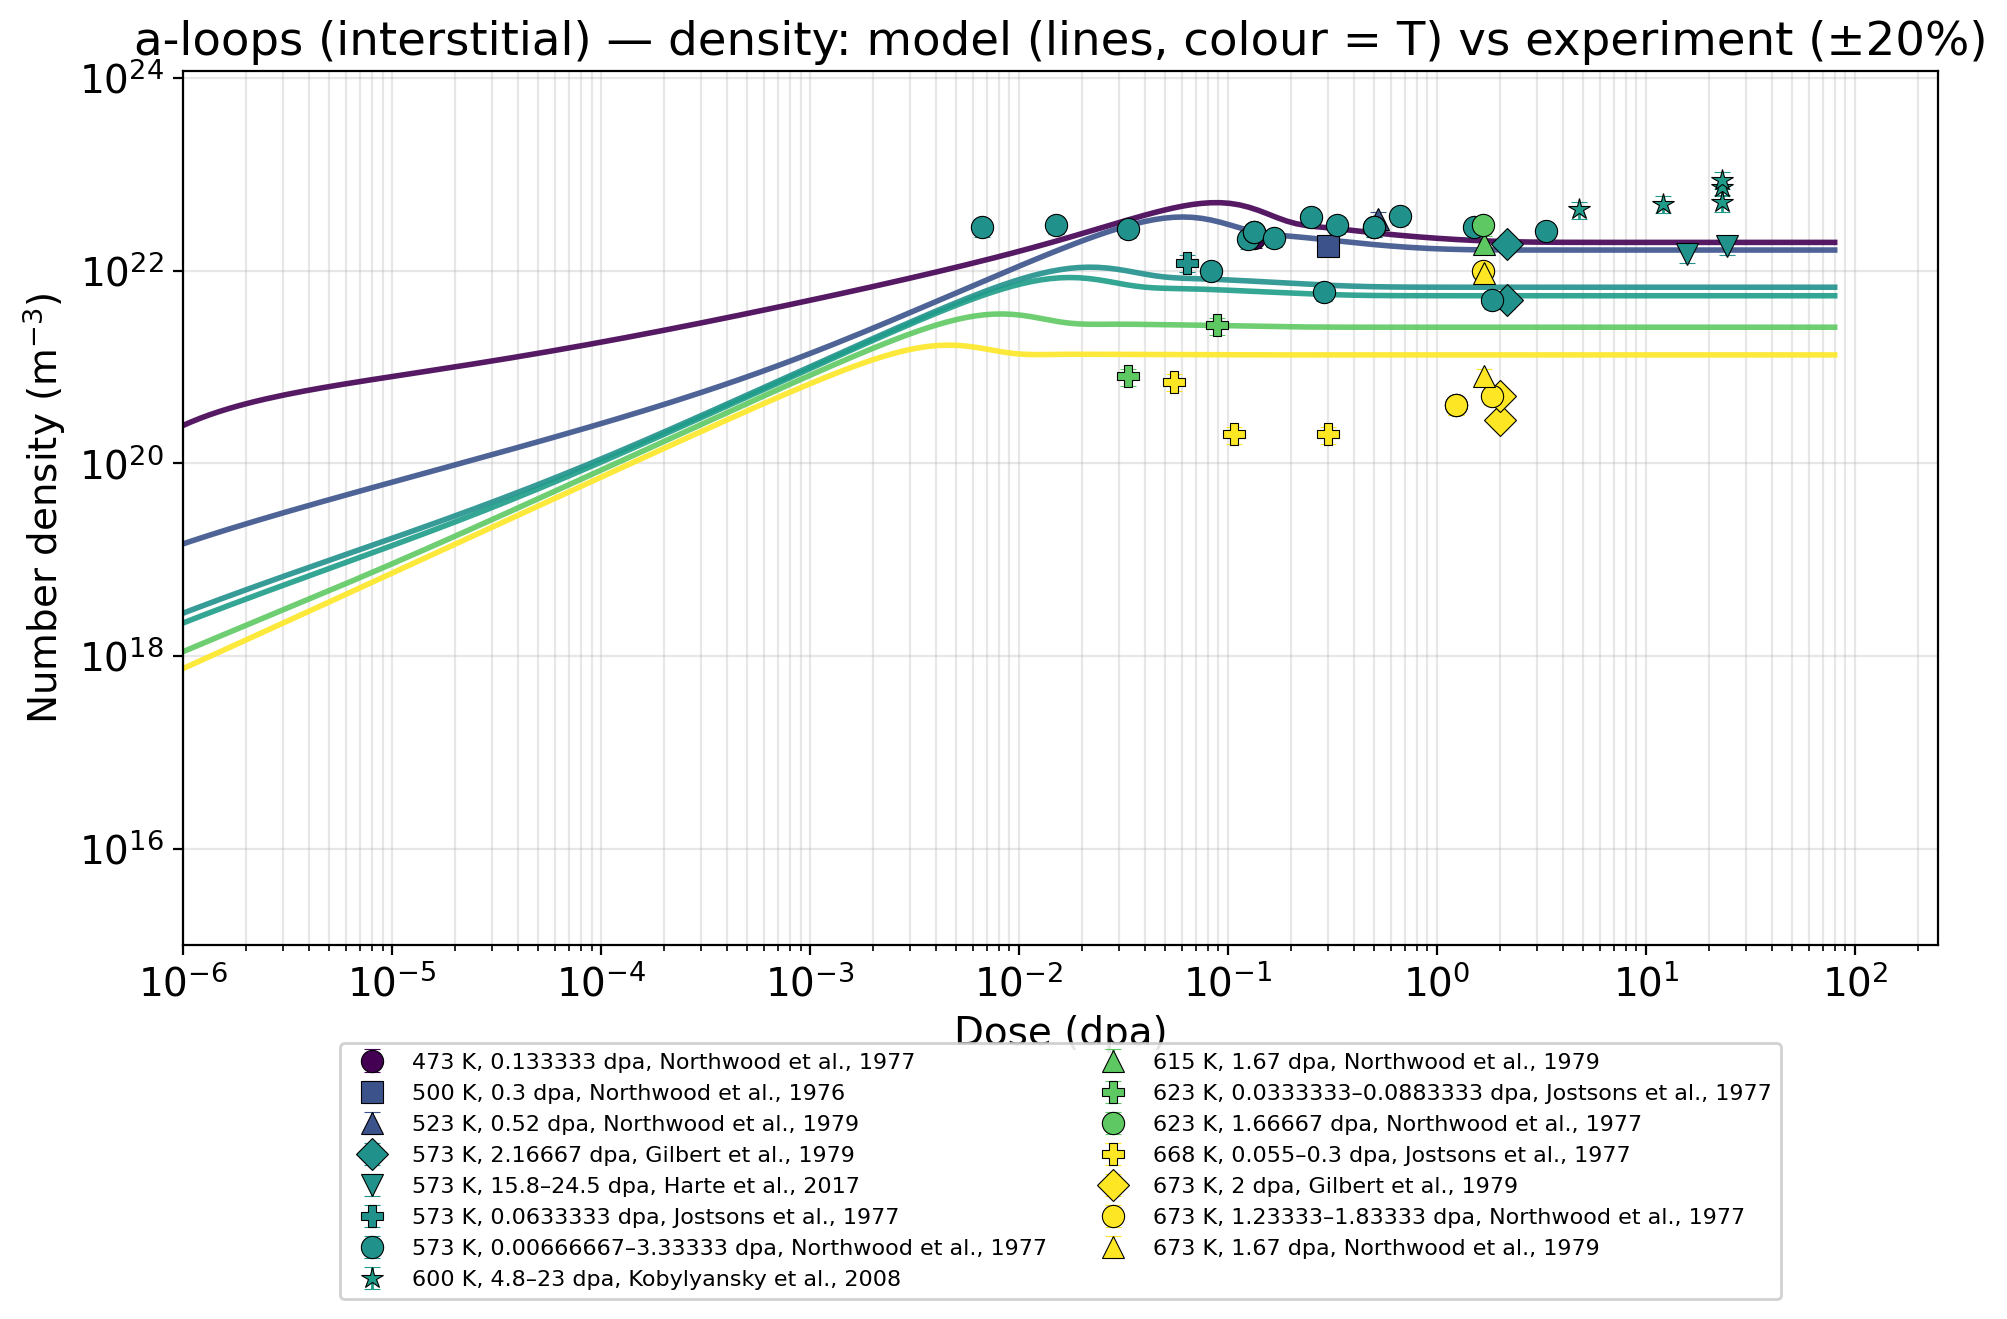
\includegraphics[width=\linewidth]{figures/aloop_density_vs_experiment.png}\\[-1pt]
  {\scriptsize (a) $a$-loop number density}
\end{minipage}\hfill
\begin{minipage}{0.49\textwidth}\centering
  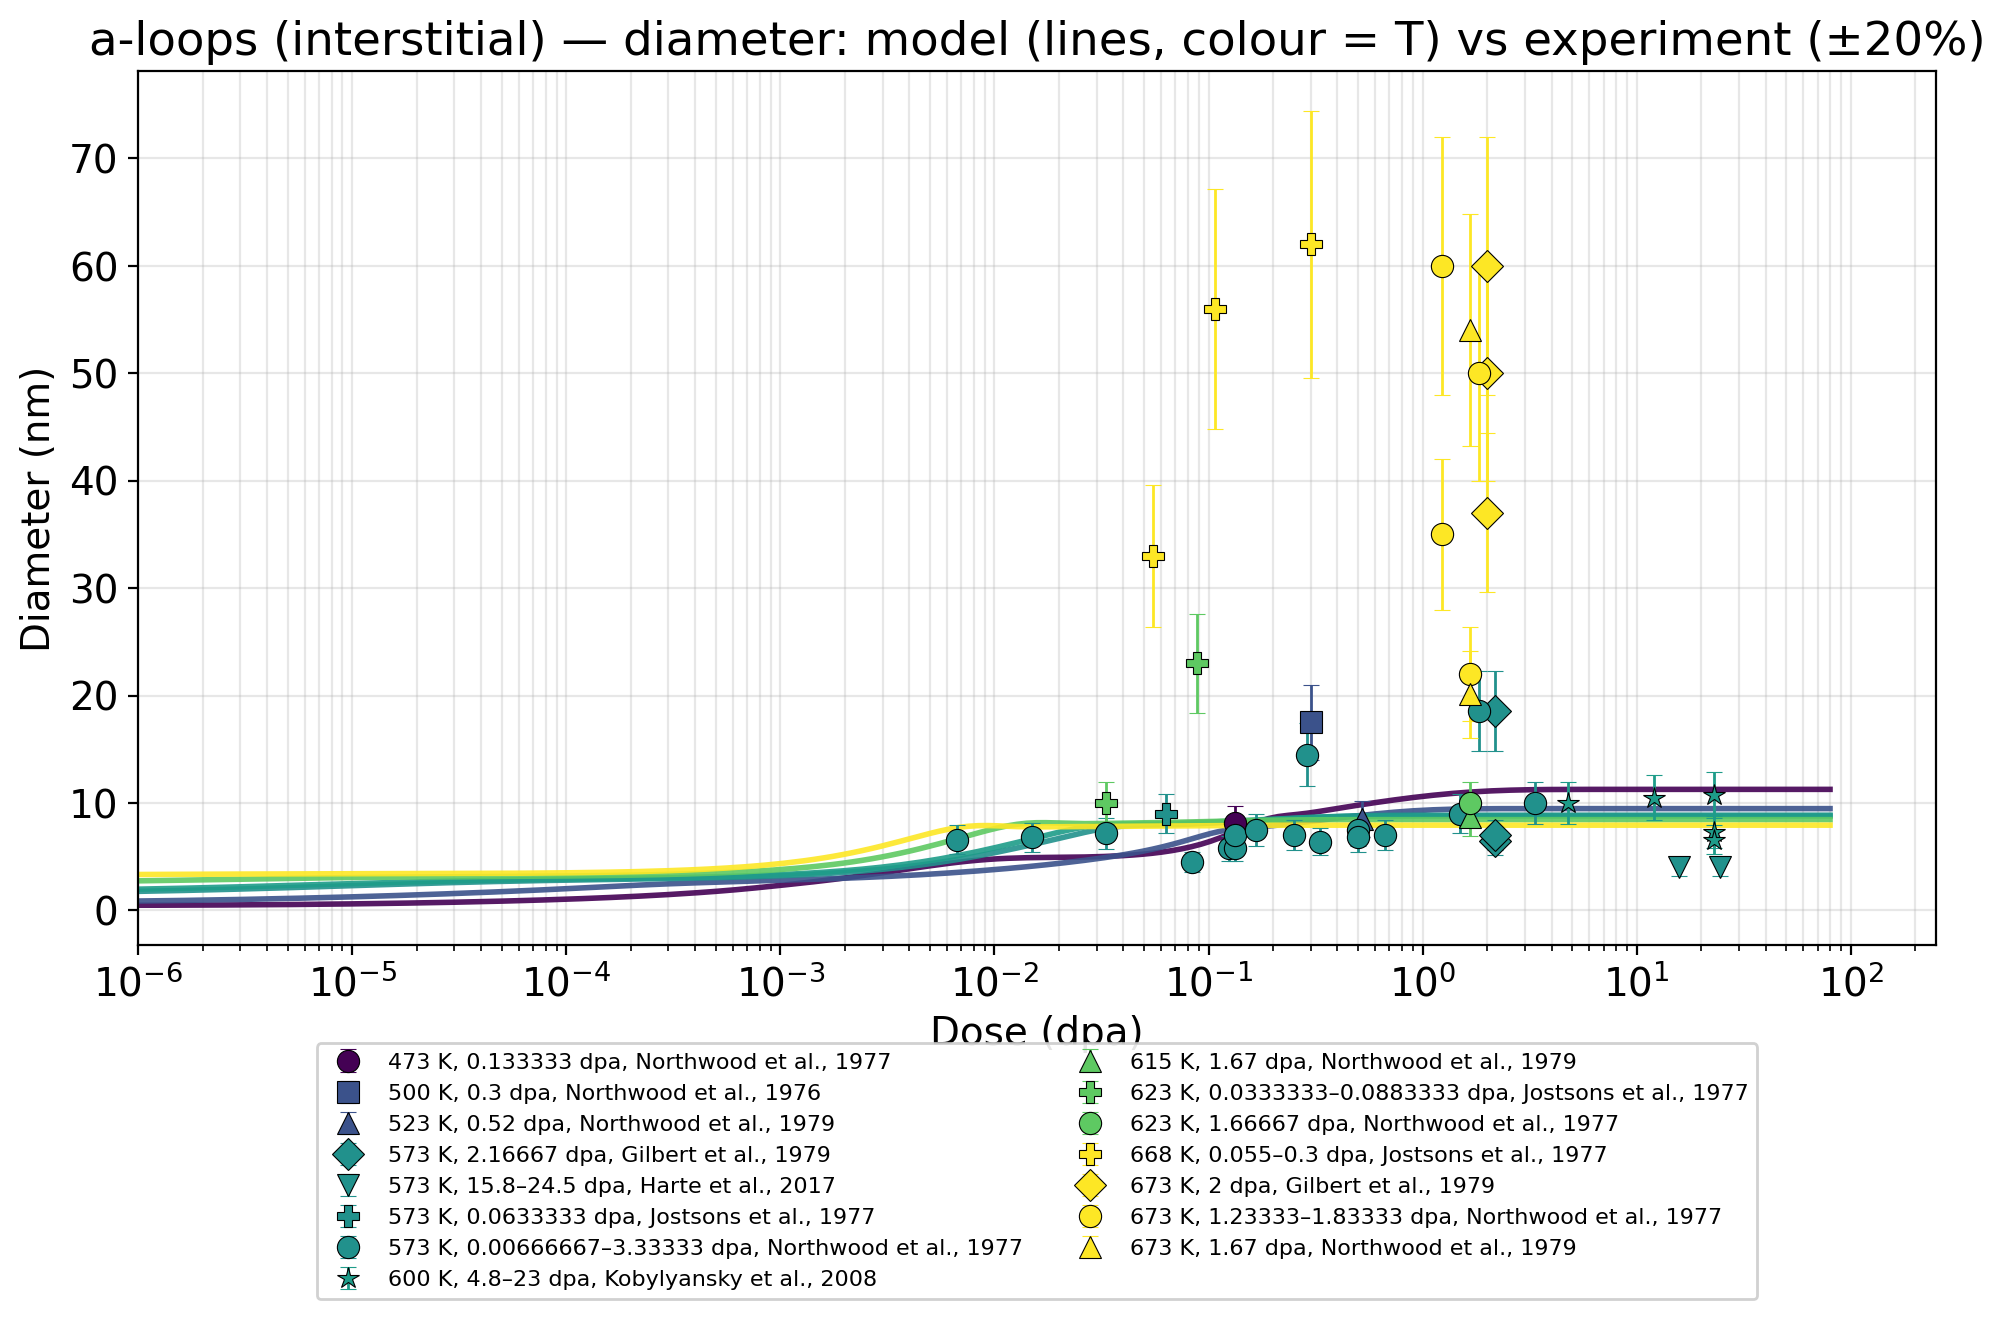
\includegraphics[width=\linewidth]{figures/aloop_diameter_vs_experiment.png}\\[-1pt]
  {\scriptsize (b) $a$-loop mean diameter}
\end{minipage}

\vspace{4pt}
\begin{minipage}{0.49\textwidth}\centering
  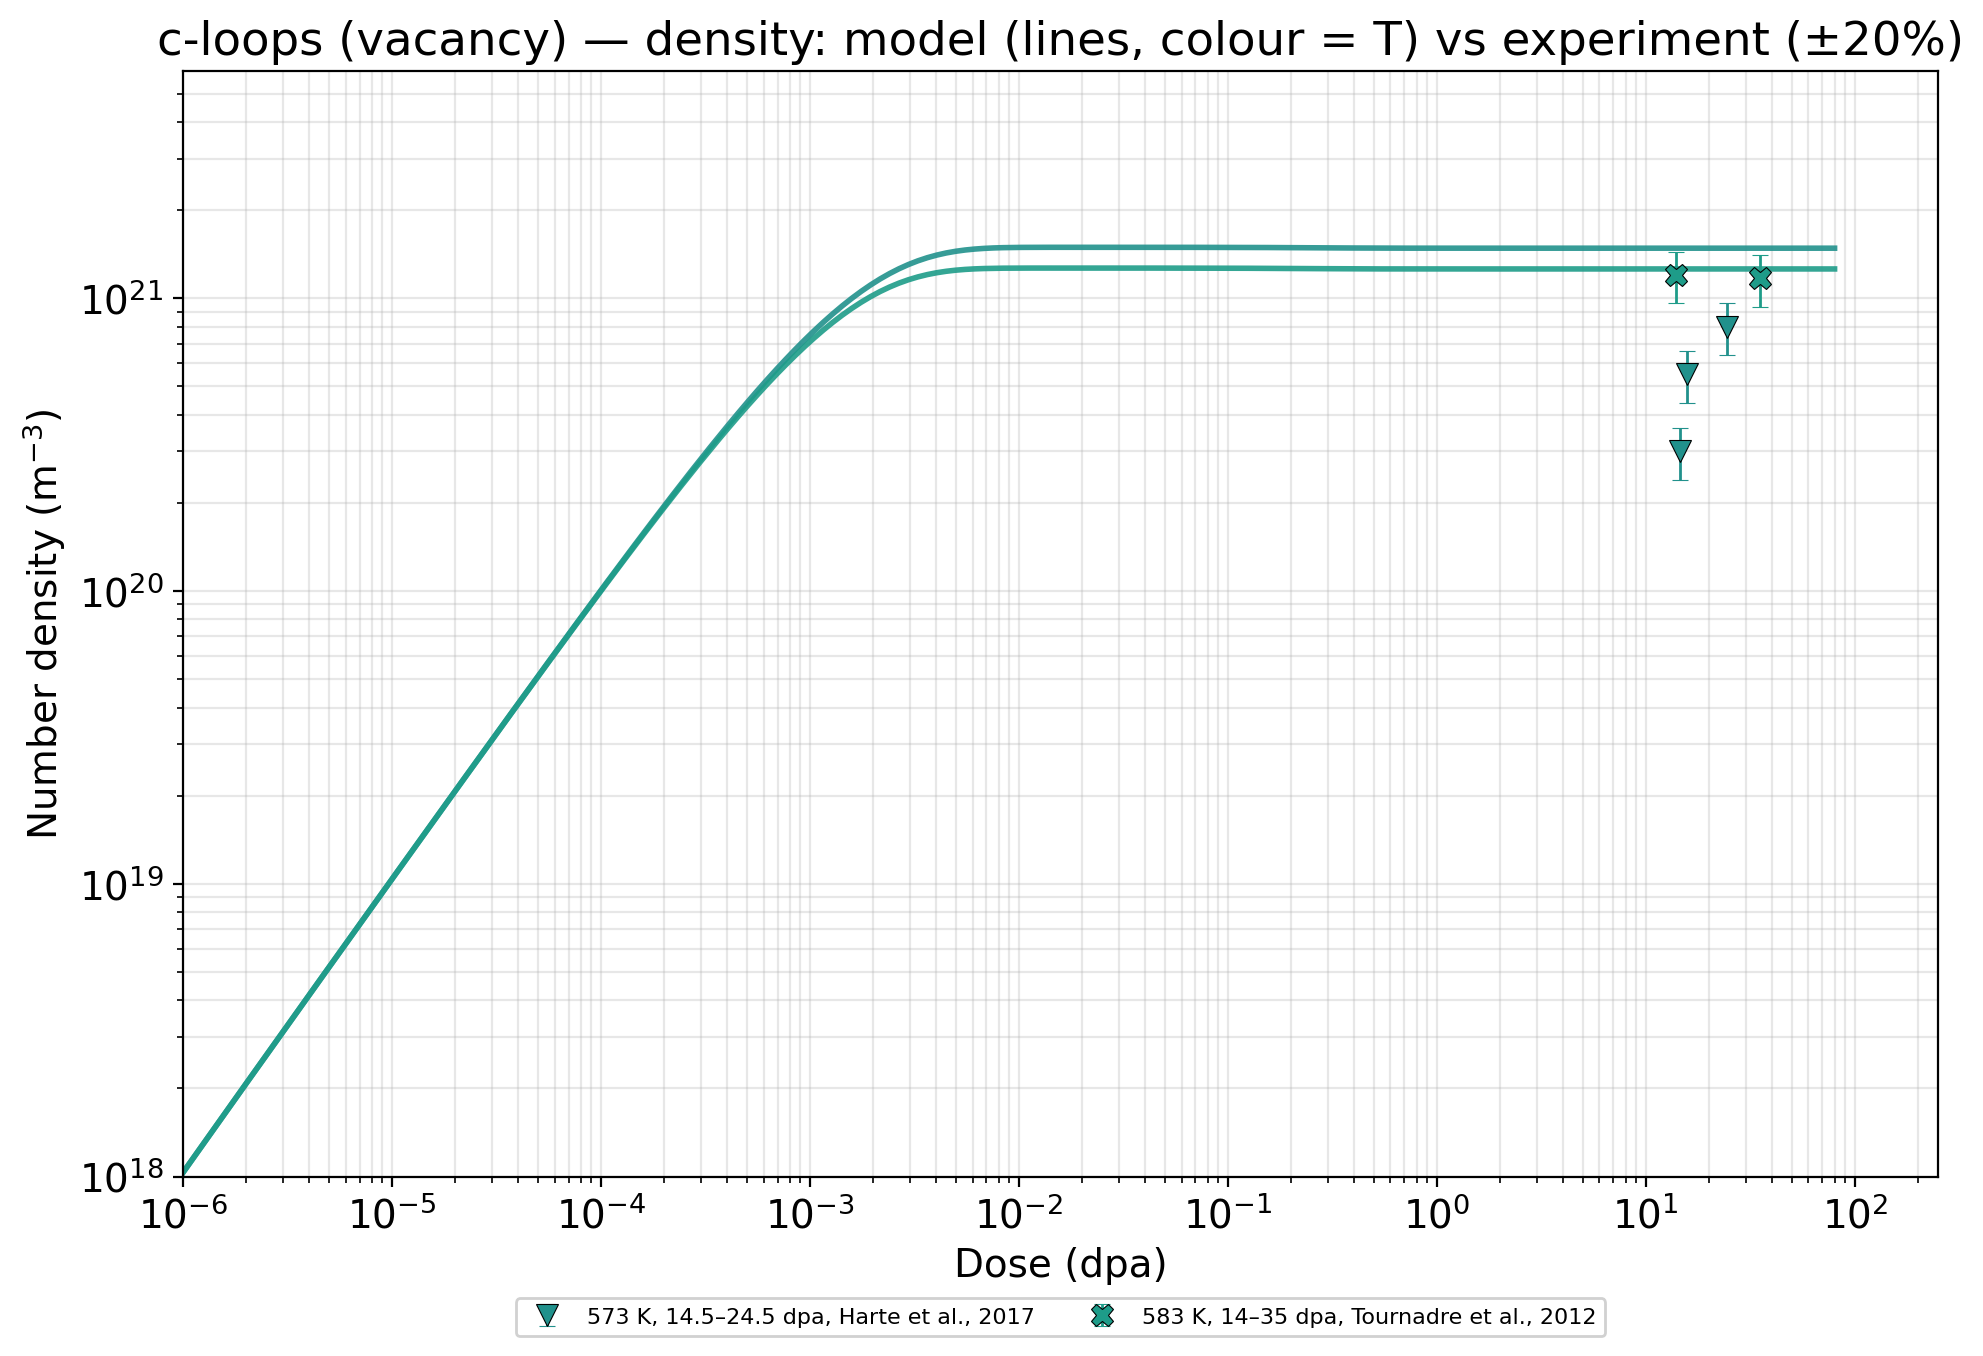
\includegraphics[width=\linewidth]{figures/cloop_density_vs_experiment.png}\\[-1pt]
  {\scriptsize (c) $c$-loop number density}
\end{minipage}\hfill
\begin{minipage}{0.49\textwidth}\centering
  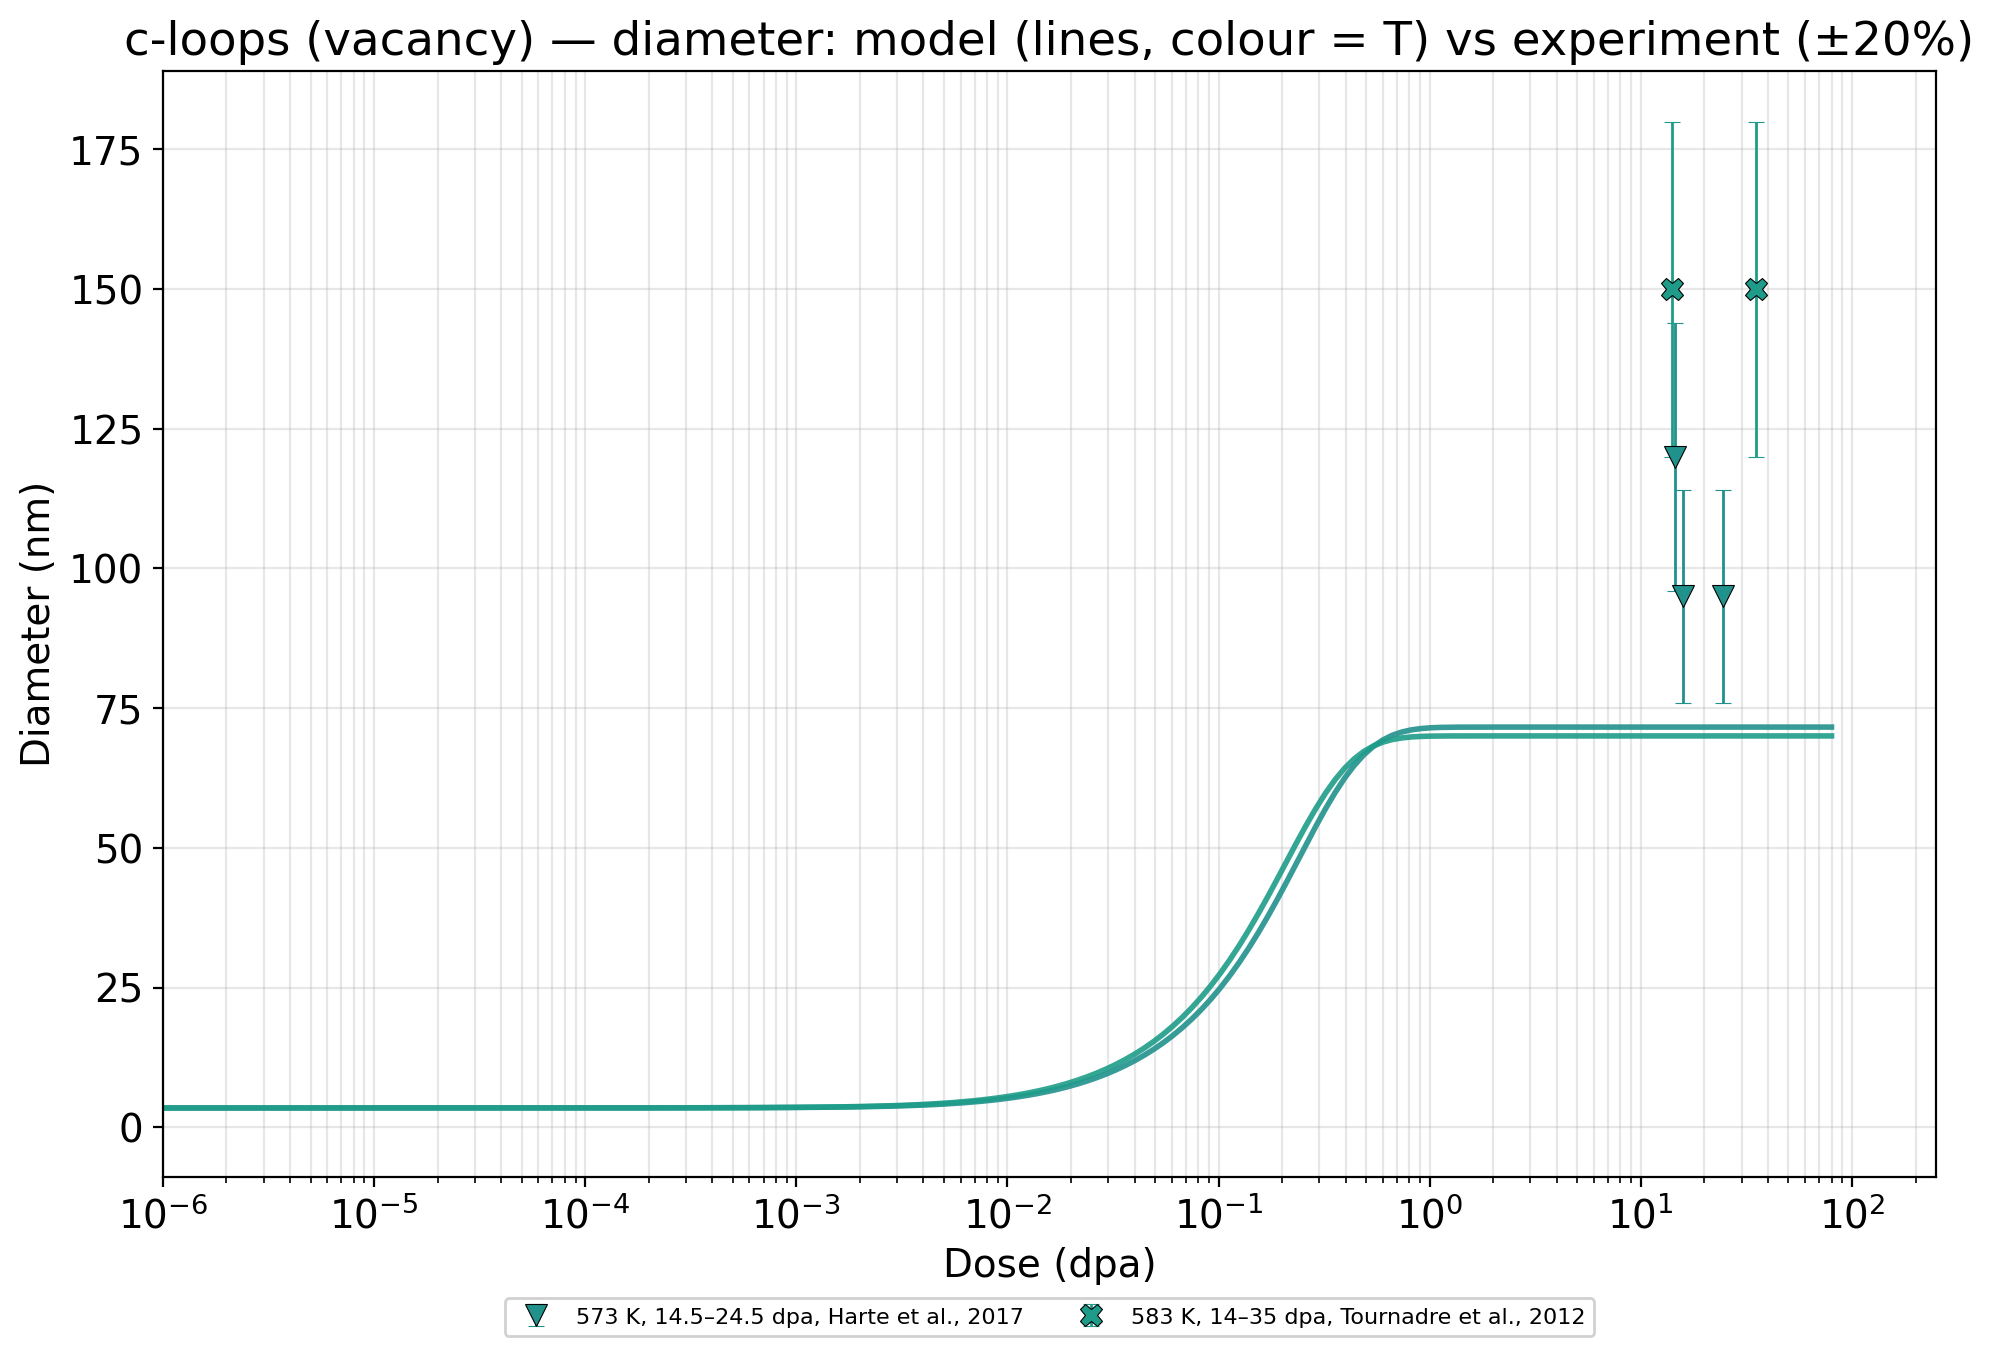
\includegraphics[width=\linewidth]{figures/cloop_diameter_vs_experiment.png}\\[-1pt]
  {\scriptsize (d) $c$-loop mean diameter}
\end{minipage}
\caption{First-round optimum: model (lines, color $=T$) versus experiment
(markers, $\pm20\%$). (a) $a$-loop density saturates at
$\sim\!1$--$2\times10^{22}\,\si{\per\cubic\metre}$, matching the dense
$473$--$623\,$K cluster and the annealed high-$T$ tail. (b) $a$-loop diameter
saturates near $10$--$15\,$nm, consistent with the low/mid-$T$ data; the large
$33$--$62\,$nm points at $668$--$673\,$K are the excluded vacancy-character
``$a$'' loops. (c) $c$-loop density saturates near
$1.3\times10^{21}\,\si{\per\cubic\metre}$, matching Tournadre ($583\,$K) and
bracketing the Harte ($573\,$K) points. (d) $c$-loop diameter saturates at
$\sim\!70\,$nm versus the measured $95$--$150\,$nm --- the model under-predicts
$c$-loop size by $\sim\!1.5$--$2\times$, the principal remaining discrepancy and
the motivation for the targeted $c$-loop refit in \texttt{fit\_cloops.py}.}
\label{fig:parity}
\end{figure}

\paragraph{Reading of the results.}
Three observations follow from Figure~\ref{fig:parity} and
Tables~\ref{tab:optimal}--\ref{tab:minimal}:
\begin{enumerate}\itemsep2pt
\item \emph{Density is well constrained; size, less so.} Both loop densities sit
inside the experimental scatter across the whole dose range; the residual is
dominated by the $c$-loop \emph{diameter} (model $70\,$nm vs. data
$\gtrsim 95\,$nm), reflecting that the $c$-loop content grows by absorbed-flux
climb and coalescence faster than the present $Q$, $c_{LN}^c$, and
$n_{vL}^{\mathrm{nuc}}$ allow.
\item \emph{The cascade-supply and birth-size levers rail.} $\varepsilon_{2i}$,
$\varepsilon_{3i}$, $n_{iL}^{\mathrm{nuc}}$, $n_{vL}^{\mathrm{nuc}}$ (and
$\varepsilon_{vL}$ at its floor) push to their bounds: the data want larger
nascent clusters/loops than the bounds permit, indicating that these bounds (not the
data) currently set those values — a flag to widen them or fix them by
independent cascade information.
\item \emph{The identifiable physics is the DAD bias and the coalescence
coefficients.} The interior optima are dominated by the orientation bias
($\delta_i^{300},\delta_i^{600},\delta_v,Z_{iL}$) and the loop-coalescence scales
($c_{LL}^a,c_{LN}^a,c_{LL}^c,c_{LN}^c$), confirming that anisotropic capture and
geometric coalescence — the two main additions over the Li–Ghoniem model —
are what the loop database actually pins down.
\end{enumerate}

\section{The \texttt{ZrMicro-0d} Model Results}


The reduced (spatially averaged, $0$D) rate-theory model integrates the coupled cluster-dynamics equations for the mobile point defects and the four loop families---interstitial ``$a$'' loops and vacancy ``$c$'' loops, each resolved into a randomly oriented population and a diffusional-anisotropy-difference (DAD) aligned population---against an evolving network dislocation density $\rho_N$. This section reports the converged trajectories obtained at the optimal parameter set of Tables~\ref{tab:optimal}--\ref{tab:minimal} and confronts them, family by family, with the assembled Zr loop, growth, and hardening database. Unless noted, all quantities are plotted against dose in displacements per atom (dpa) on a logarithmic scale spanning $10^{-6}$ to $10^{2}\,$dpa, so that the nucleation transient, the overshoot, and the saturation plateau are all visible on a single axis. The recurring qualitative pattern---an early power-law build-up, a mild overshoot near $10^{-2}\,$dpa, and a temperature-controlled saturation plateau---is the signature of the balance between cascade production, mutual recombination, and biased absorption at the growing sink population, and it reproduces the canonical behavior seen in the irradiated-Zr literature.

\subsection{Point-defect kinetics}

Figure~\ref{fig:point_defects} shows the evolution of the mobile and trapped defect concentrations. The free vacancy concentration $C_v$ rises first and saturates near $5\times10^{17}\,\si{\per\cubic\centi\metre}$, while the free interstitial concentration $C_i$ remains two to three orders of magnitude lower because the faster-migrating interstitials are absorbed almost as quickly as they are produced; the di- and tri-interstitial clusters ($C_{2i},C_{3i}$) stay flat and subdominant, confirming that small mobile clusters are not a significant storage channel. The defect content bound in loops behaves oppositely: the interstitials stored in $a$-loops and the vacancies stored in $c$-loops climb steeply from $\sim\!10^{14}$ to $\sim\!10^{20}\,\si{\per\cubic\centi\metre}$ across $10^{-3}$--$1\,$dpa and then plateau, so that by saturation essentially all of the retained damage resides in the loop microstructure rather than in the matrix. This separation of the free and trapped populations is the physical basis of the partitioning used in the growth and hardening calculations.

\begin{figure}[htbp]
\centering
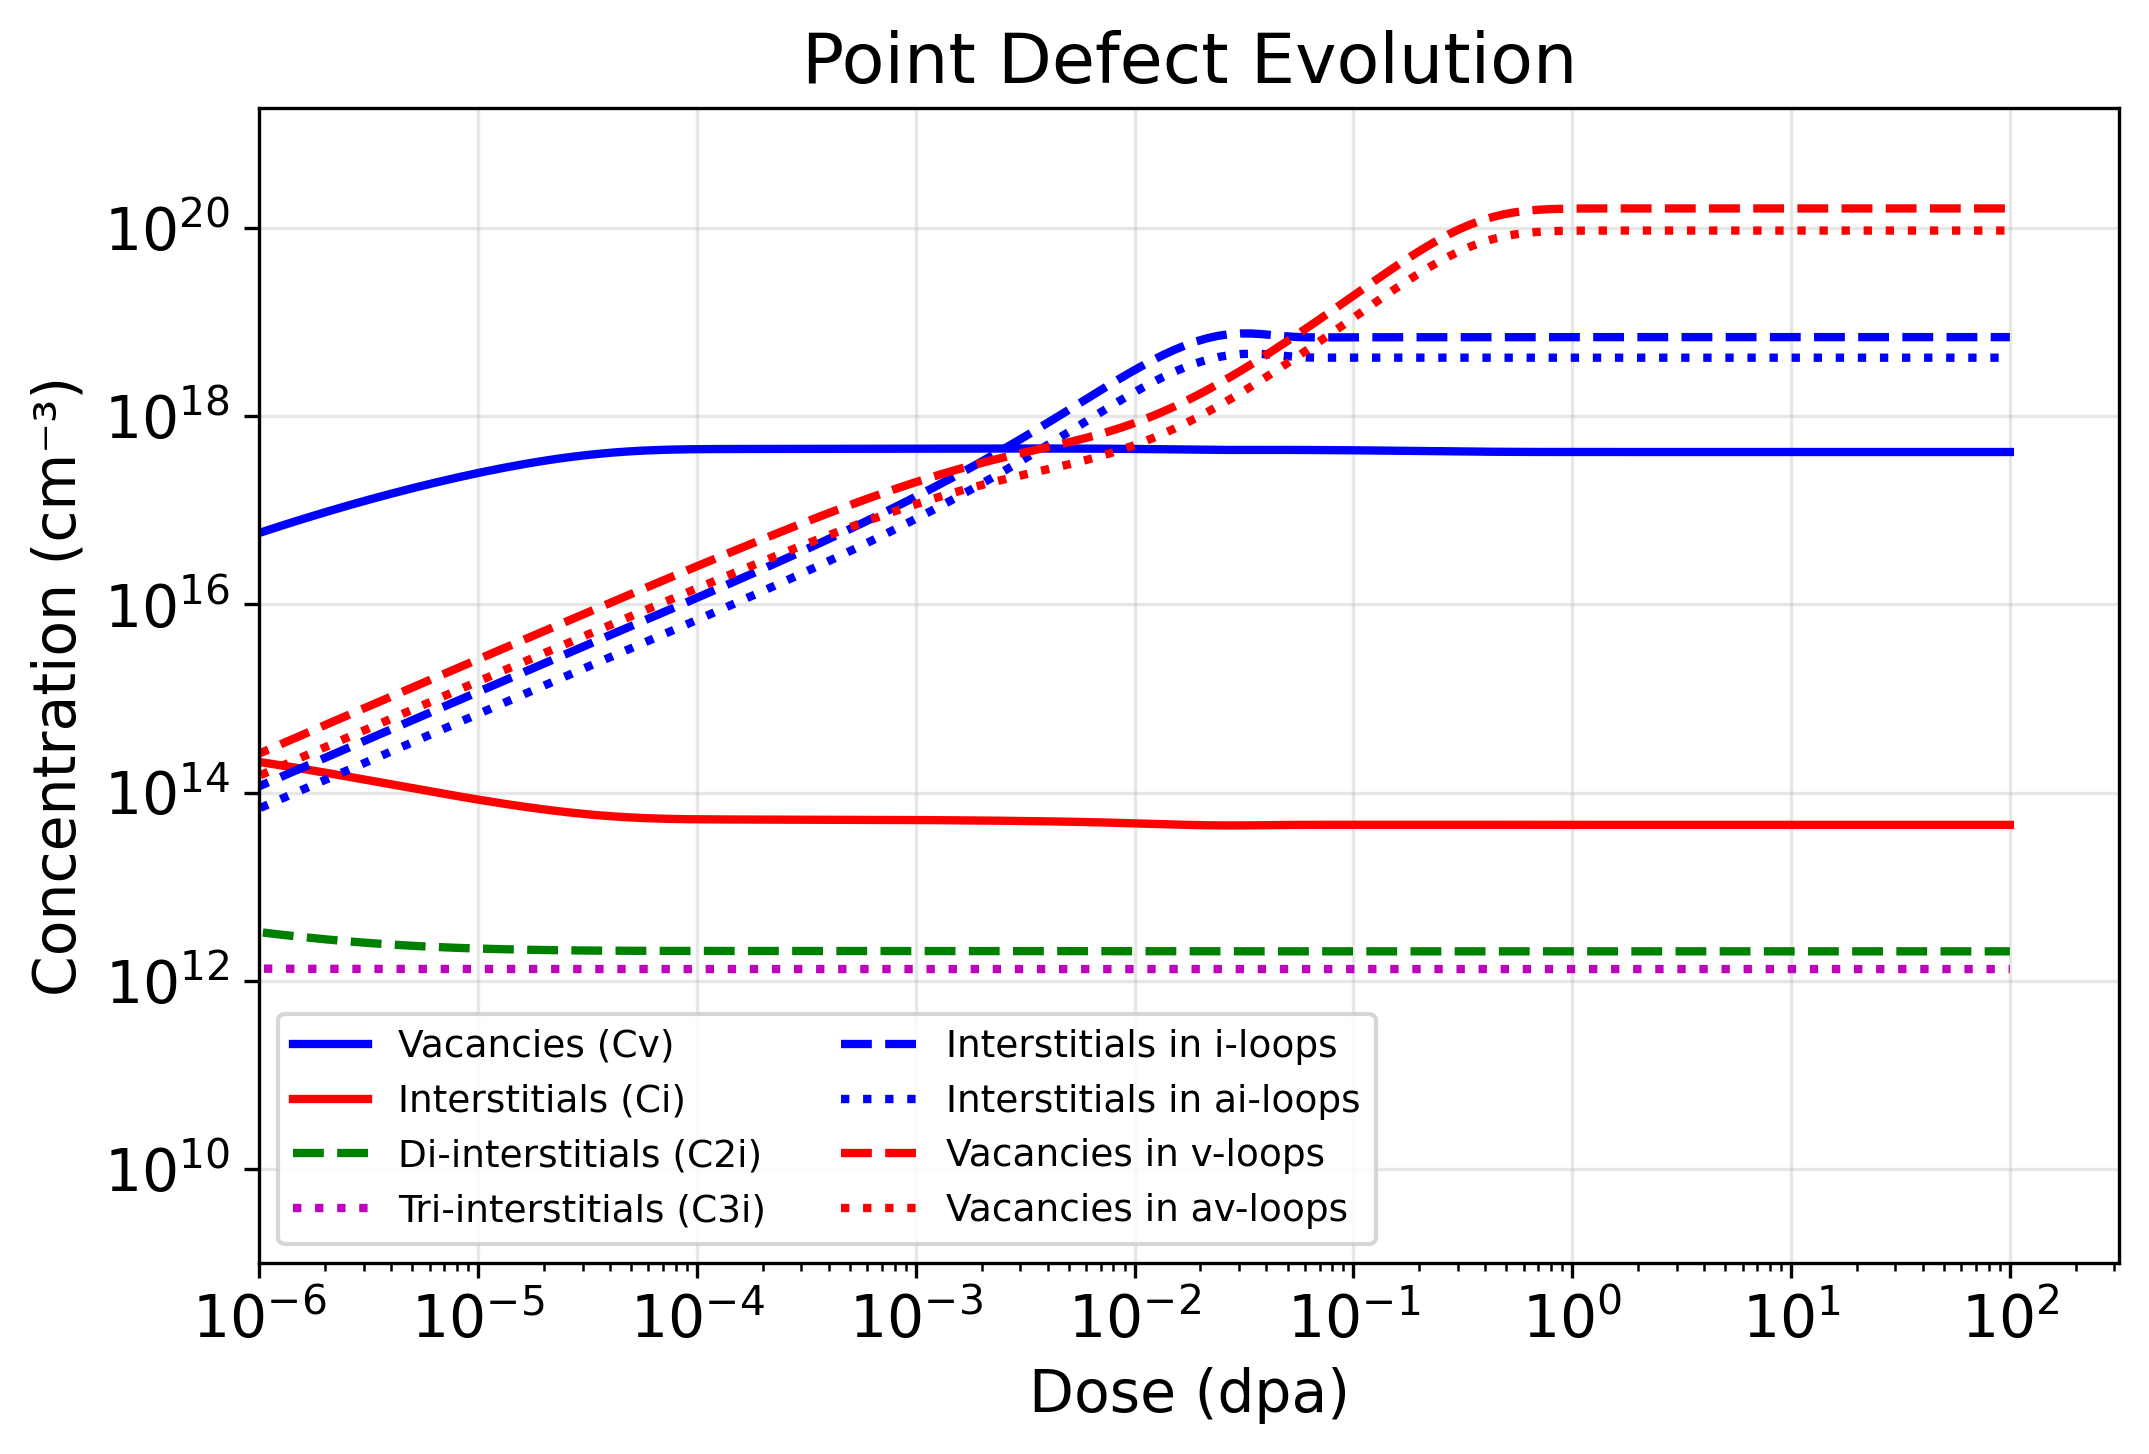
\includegraphics[width=0.7\linewidth]{figures/point_defects.png}
\caption{Point-defect evolution. Free vacancies ($C_v$) saturate near $5\times10^{17}\,\si{\per\cubic\centi\metre}$ while free interstitials ($C_i$) sit well below them; the di-/tri-interstitial channels remain negligible. The interstitial content of $a$-loops and the vacancy content of $c$-loops grow by several orders of magnitude before saturating, showing that the retained damage is overwhelmingly stored in the loop population.}
\label{fig:point_defects}
\end{figure}

The total stored-defect curve of Figure~\ref{fig:total_defect_evolution} aggregates these channels and makes the buildup,overshoot, and saturation sequence explicit, while Figure~\ref{fig:interstitial_fractions}  resolves how the interstitial budget is apportioned between the randomly oriented and DAD-aligned loop sets. The aligned fractions stabilize at the values set by the orientation bias, which is precisely the partition that produces a net directional strain. Figure~\ref{fig:defect_imbalance} plots the running difference between vacancies and interstitials delivered to the sinks; the small but nonzero, sign-definite imbalance is the engine of irradiation growth, and its saturation mirrors the saturation of the loop populations.

\begin{figure}[htbp]
\centering
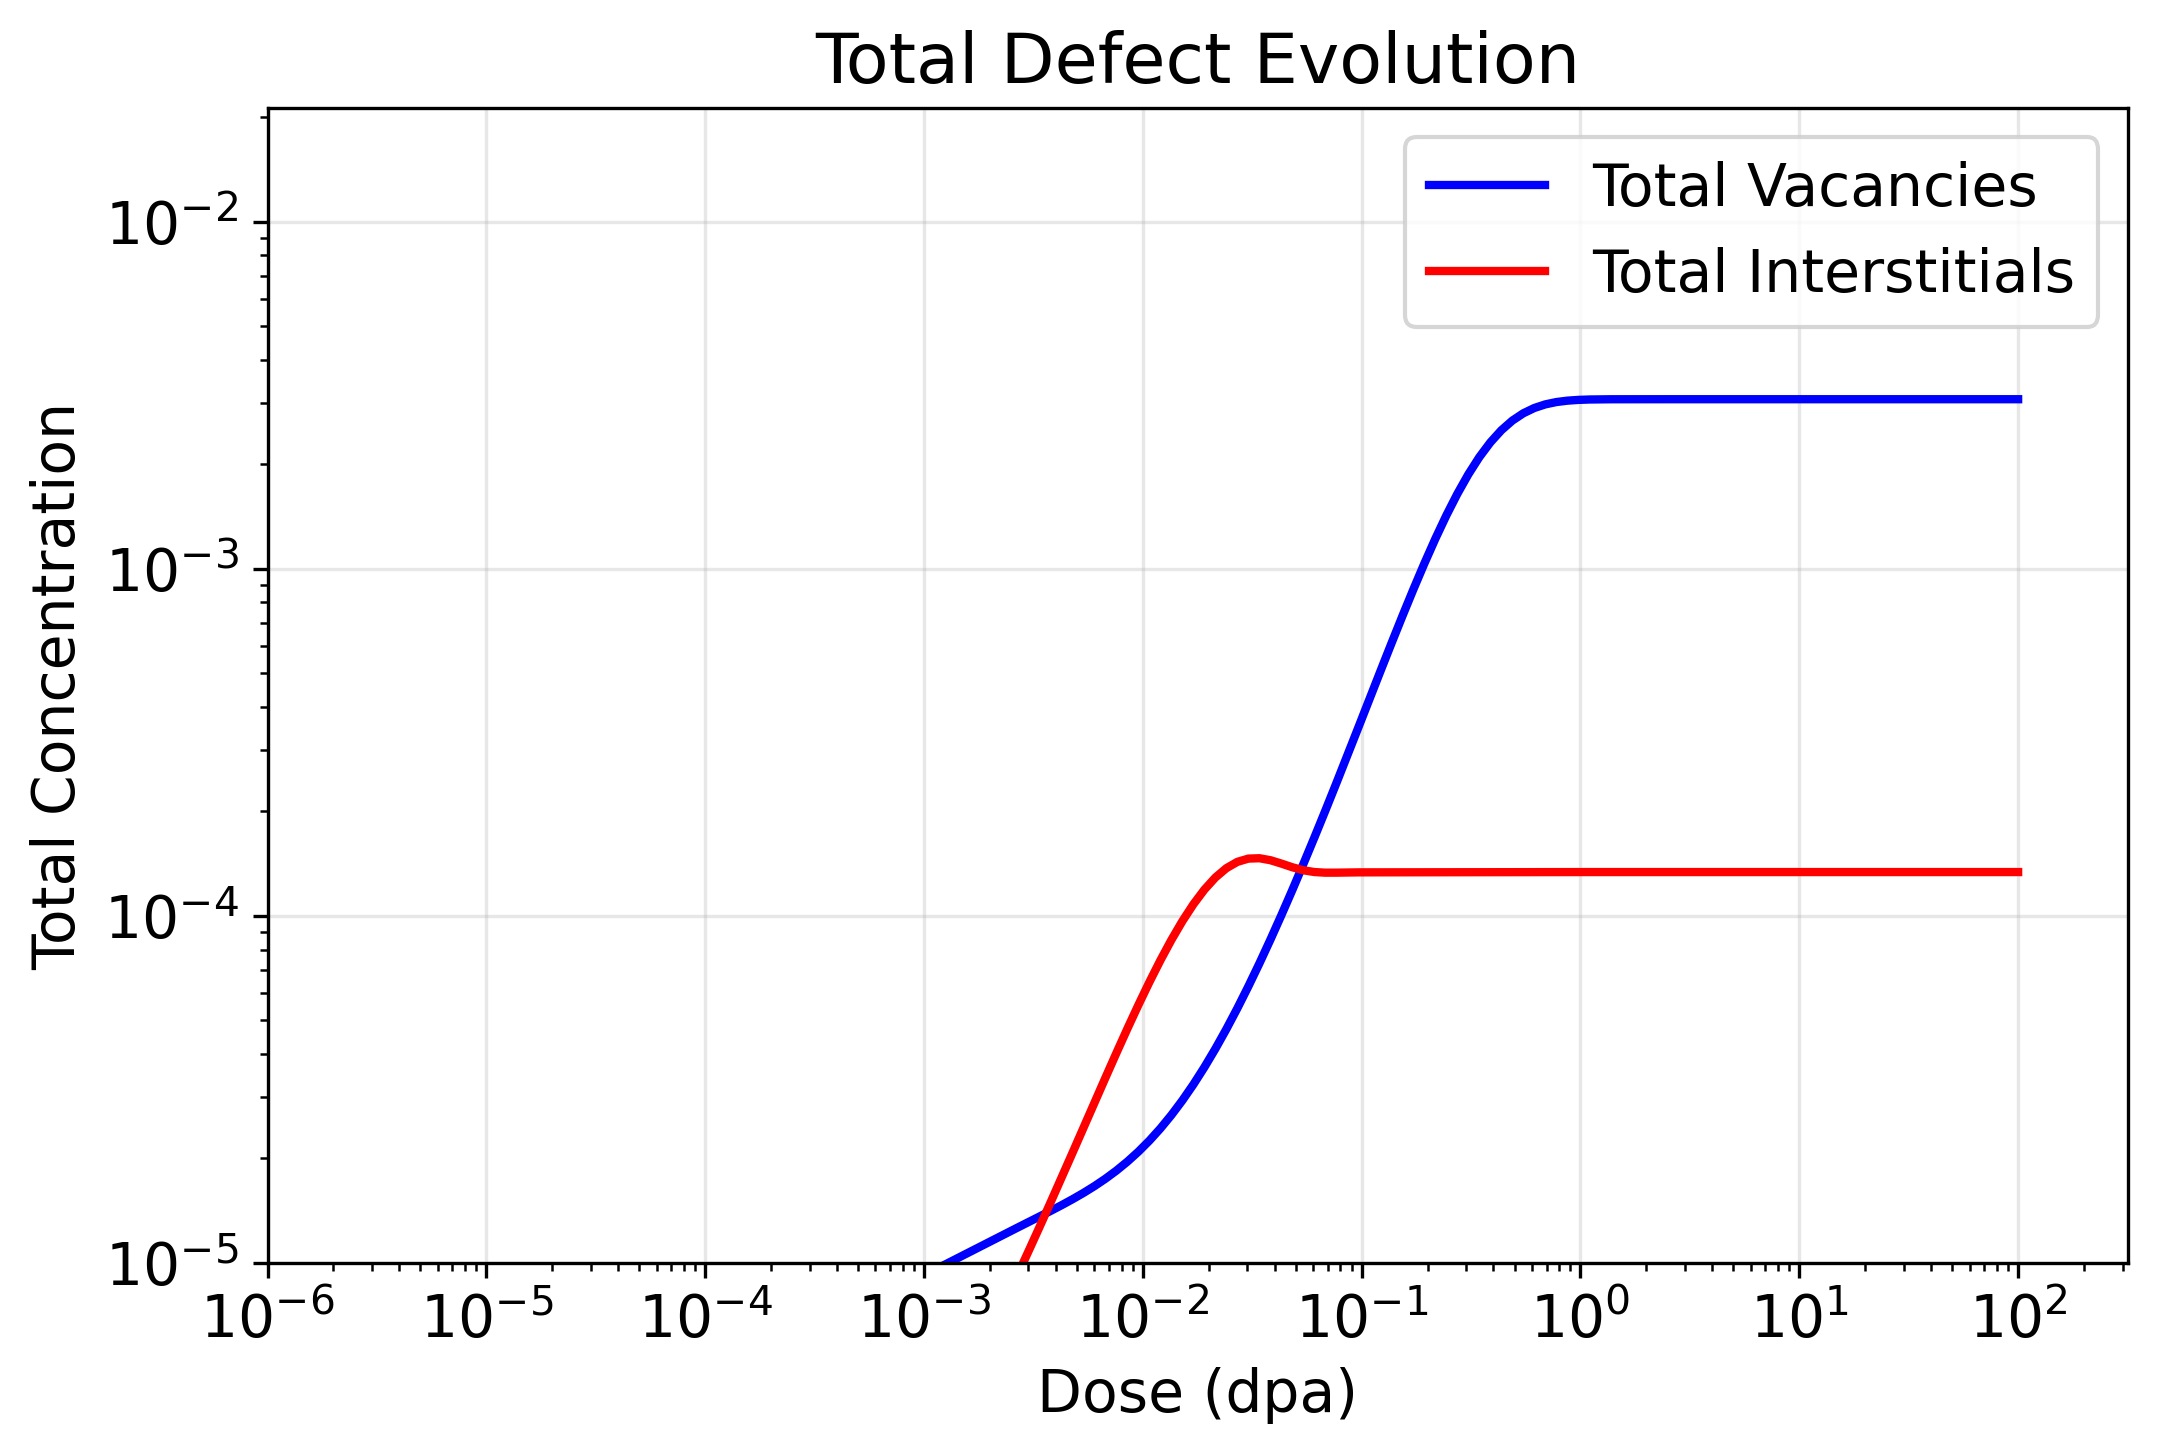
\includegraphics[width=0.7\linewidth]{figures/total_defect_evolution.png}
\caption{Total stored-defect evolution versus dose, showing the early build-up, the mild overshoot near $10^{-2}\,$dpa, and the saturation plateau that is inherited by all downstream microstructural quantities.}
\label{fig:total_defect_evolution}
\end{figure}

\begin{figure}[htbp]
\centering
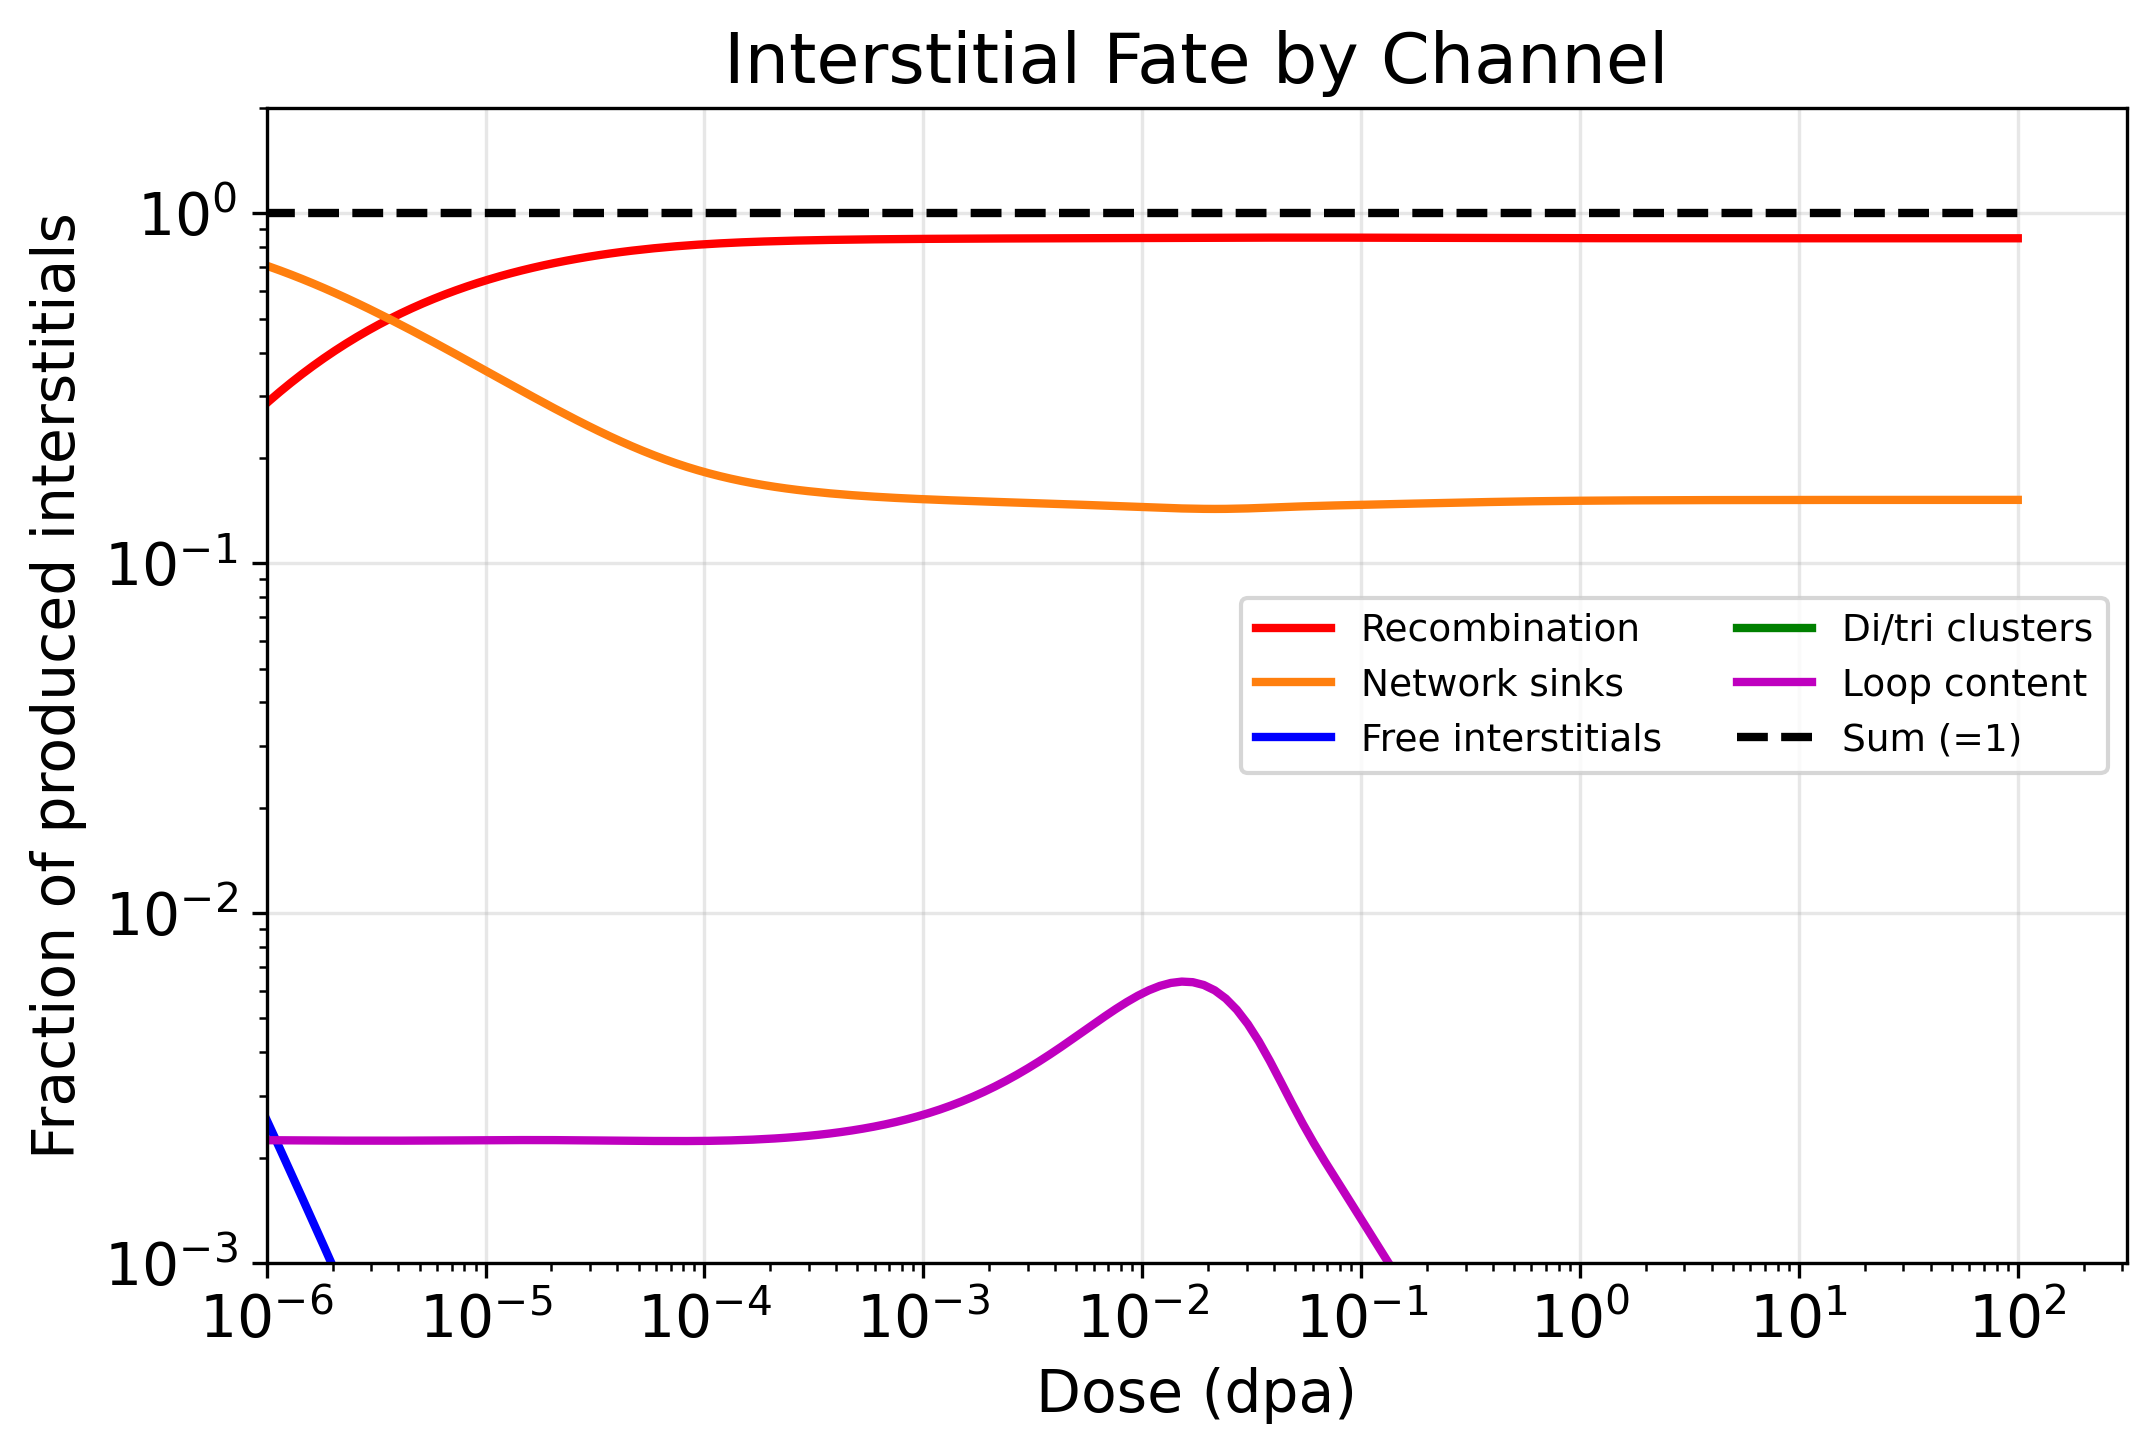
\includegraphics[width=0.49\linewidth]{figures/interstitial_fractions.png}
\hfill
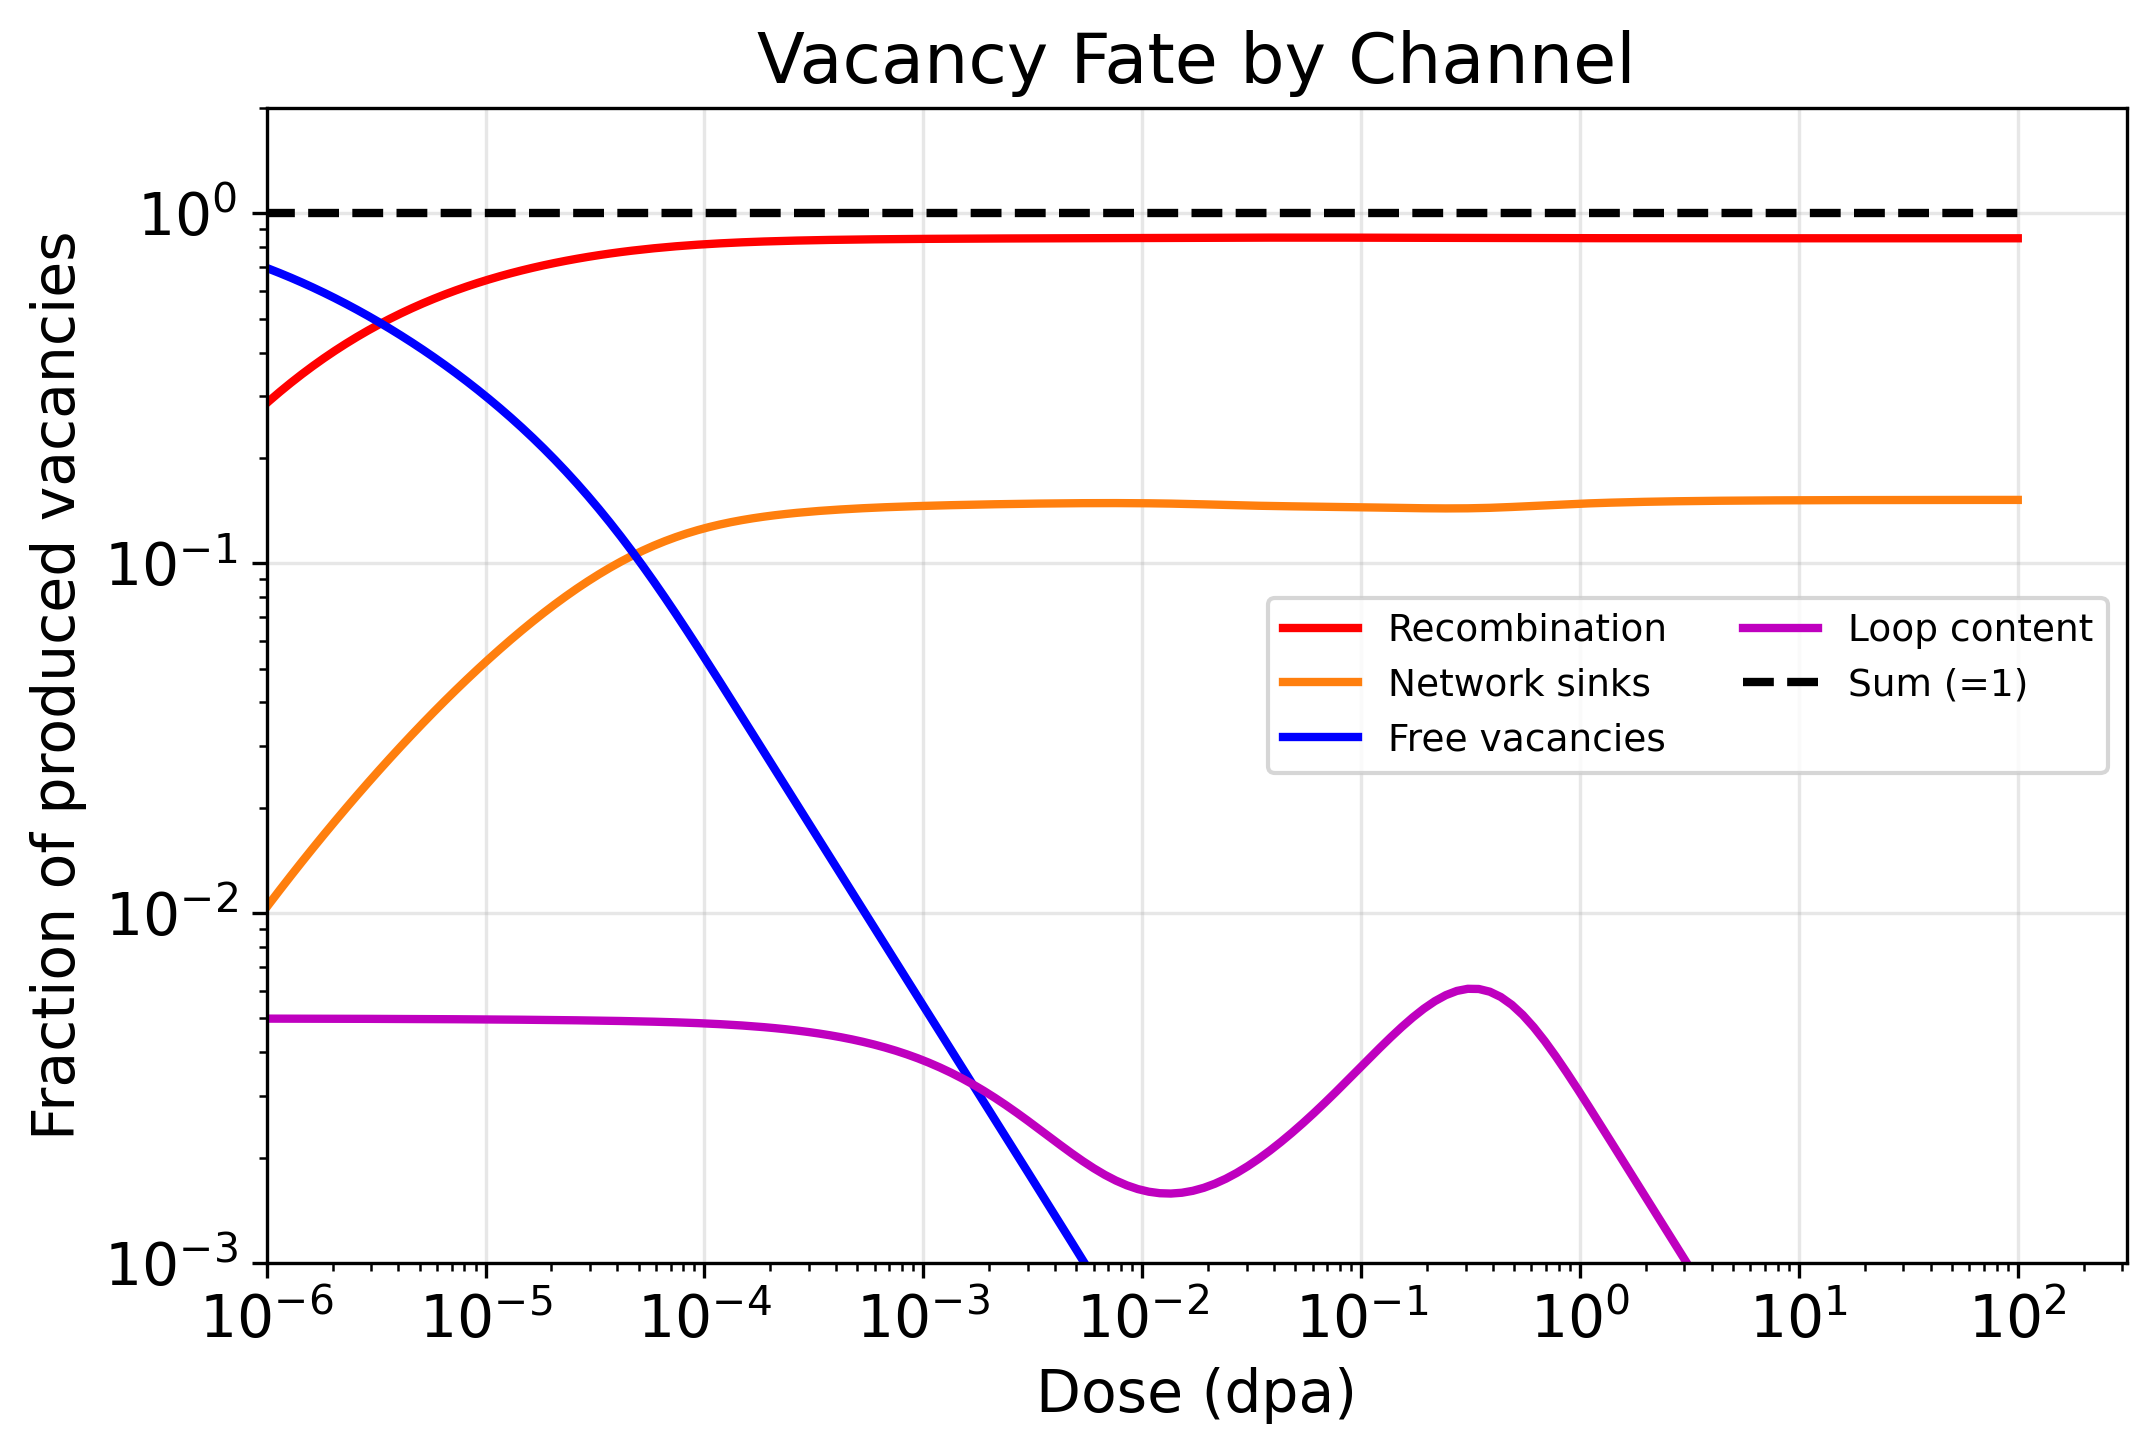
\includegraphics[width=0.49\linewidth]{figures/vacancy_fractions.png}
\caption{Partition of the interstitial (left) and vacancy (right) budgets between the randomly oriented and DAD-aligned loop populations. The aligned fractions settle to the values fixed by the orientation bias, supplying the directional sink strength that drives growth.}
\label{fig:interstitial_fractions}
\end{figure}

\begin{figure}[htbp]
\centering
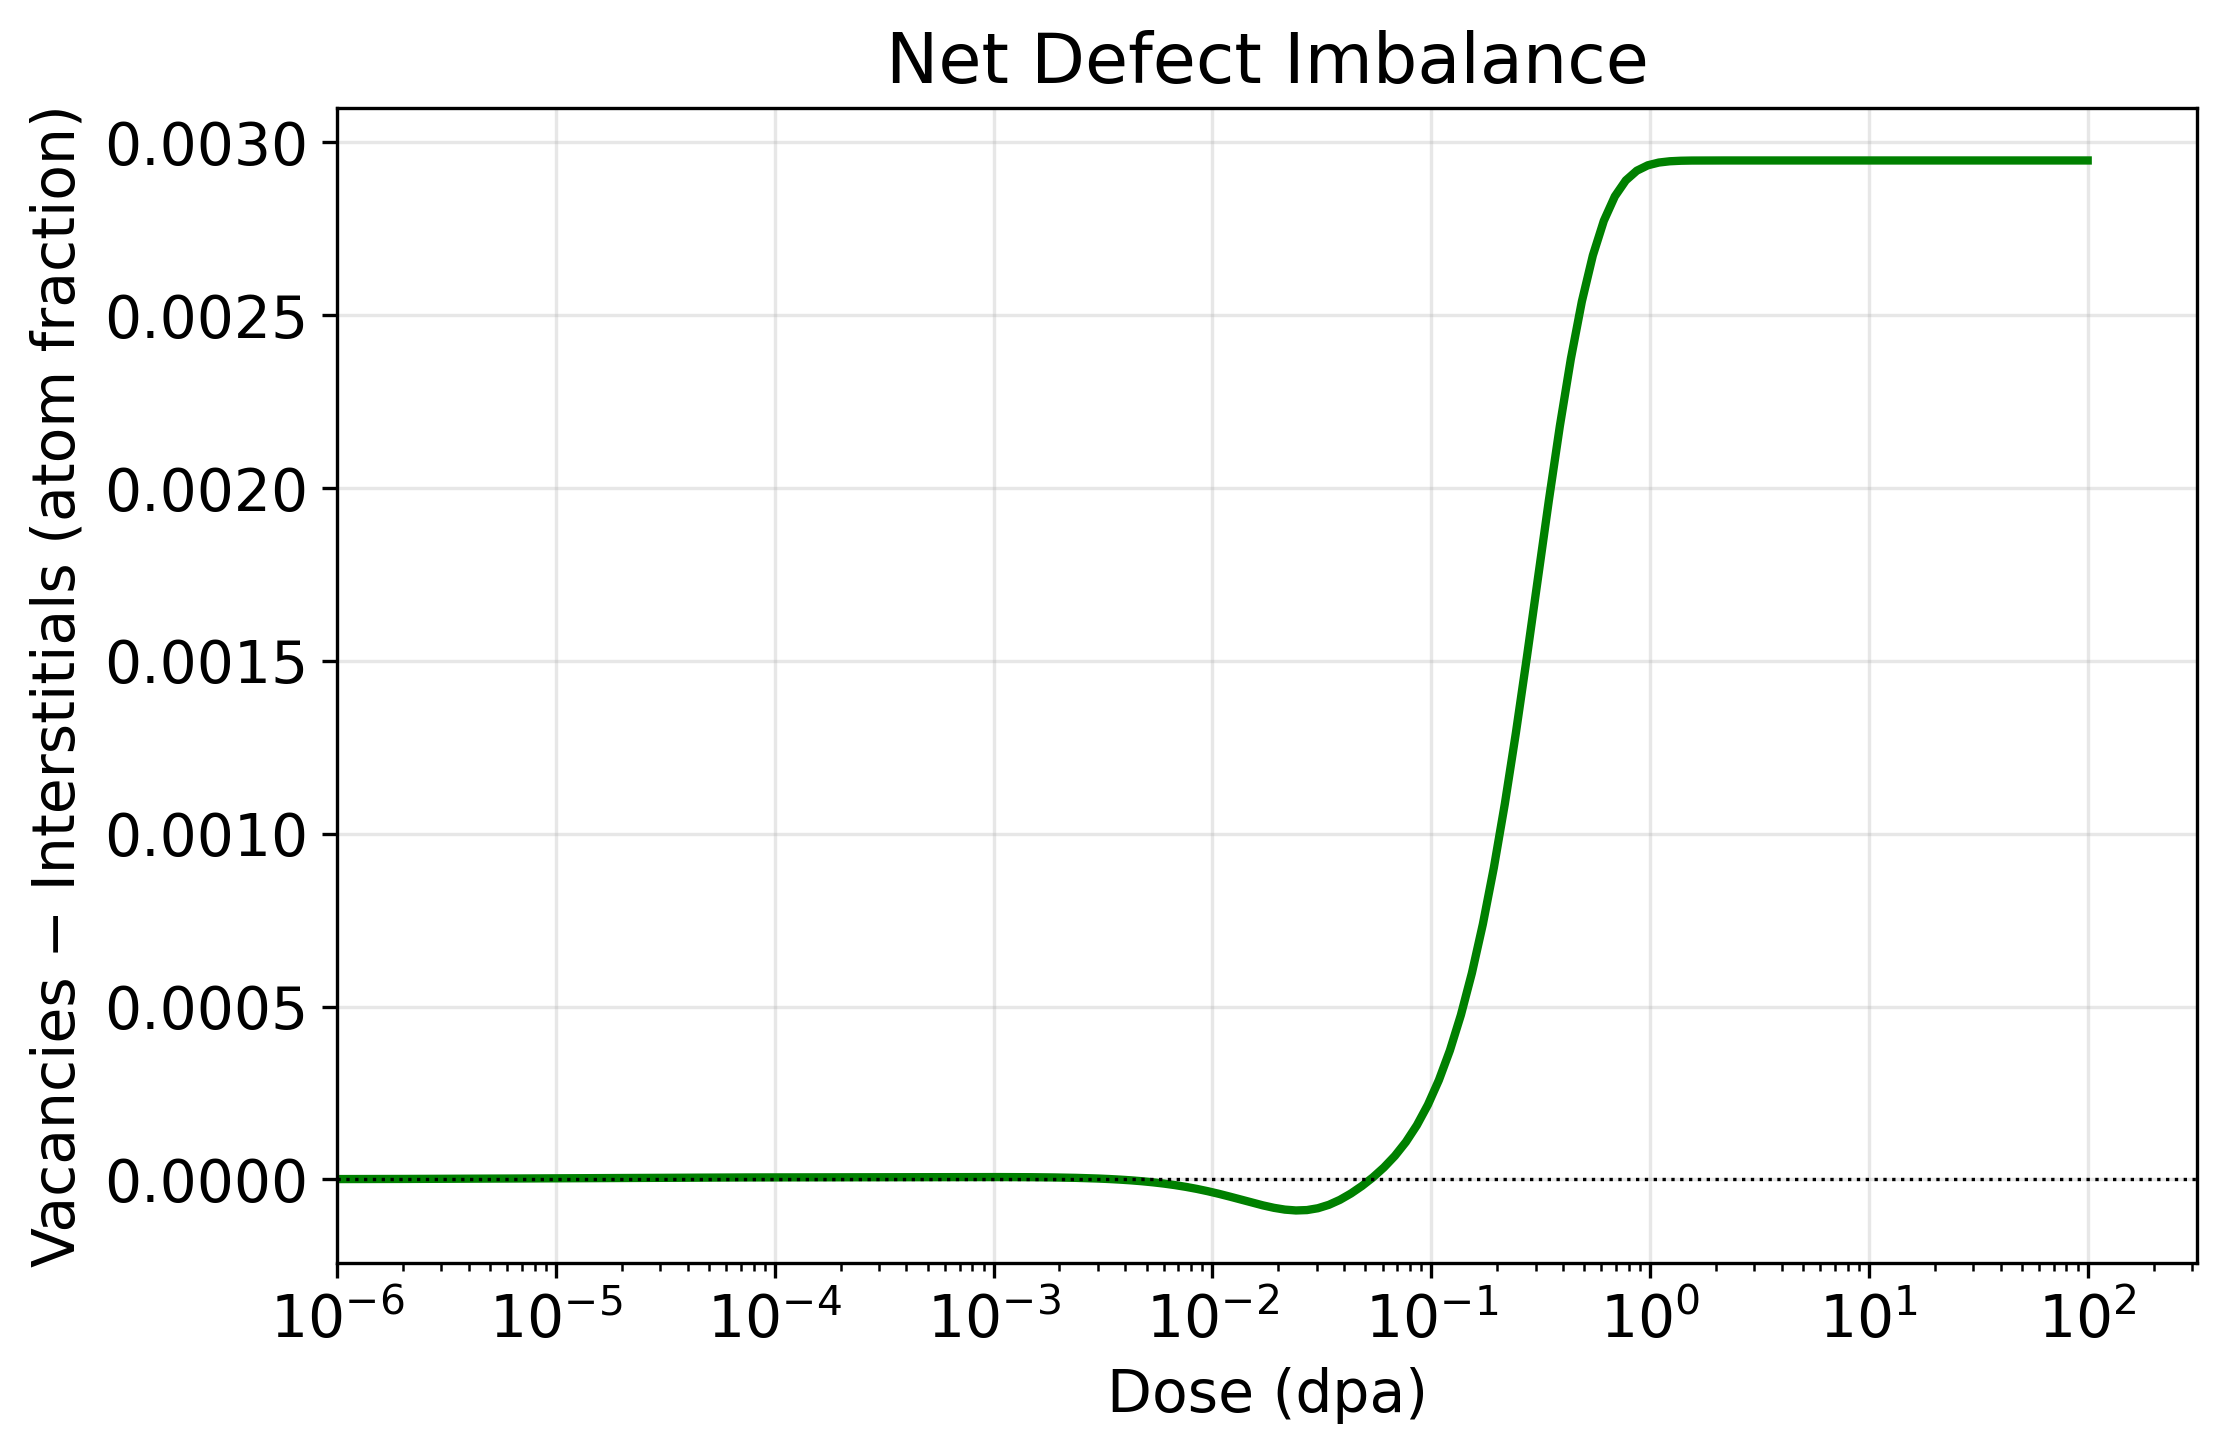
\includegraphics[width=0.7\linewidth]{figures/defect_imbalance.png}
\caption{Net vacancy--interstitial imbalance arriving at the sinks. The sign-definite, saturating imbalance is the microscopic driver of the macroscopic growth strain.}
\label{fig:defect_imbalance}
\end{figure}

The remaining transport diagnostics confirm that the integration is physically self-consistent. Figure~\ref{fig:flux_evolution} tracks the absolute vacancy and interstitial fluxes to the sinks as they rise during the transient and lock together once the sink strength saturates. 

\begin{figure}[htbp]
\centering
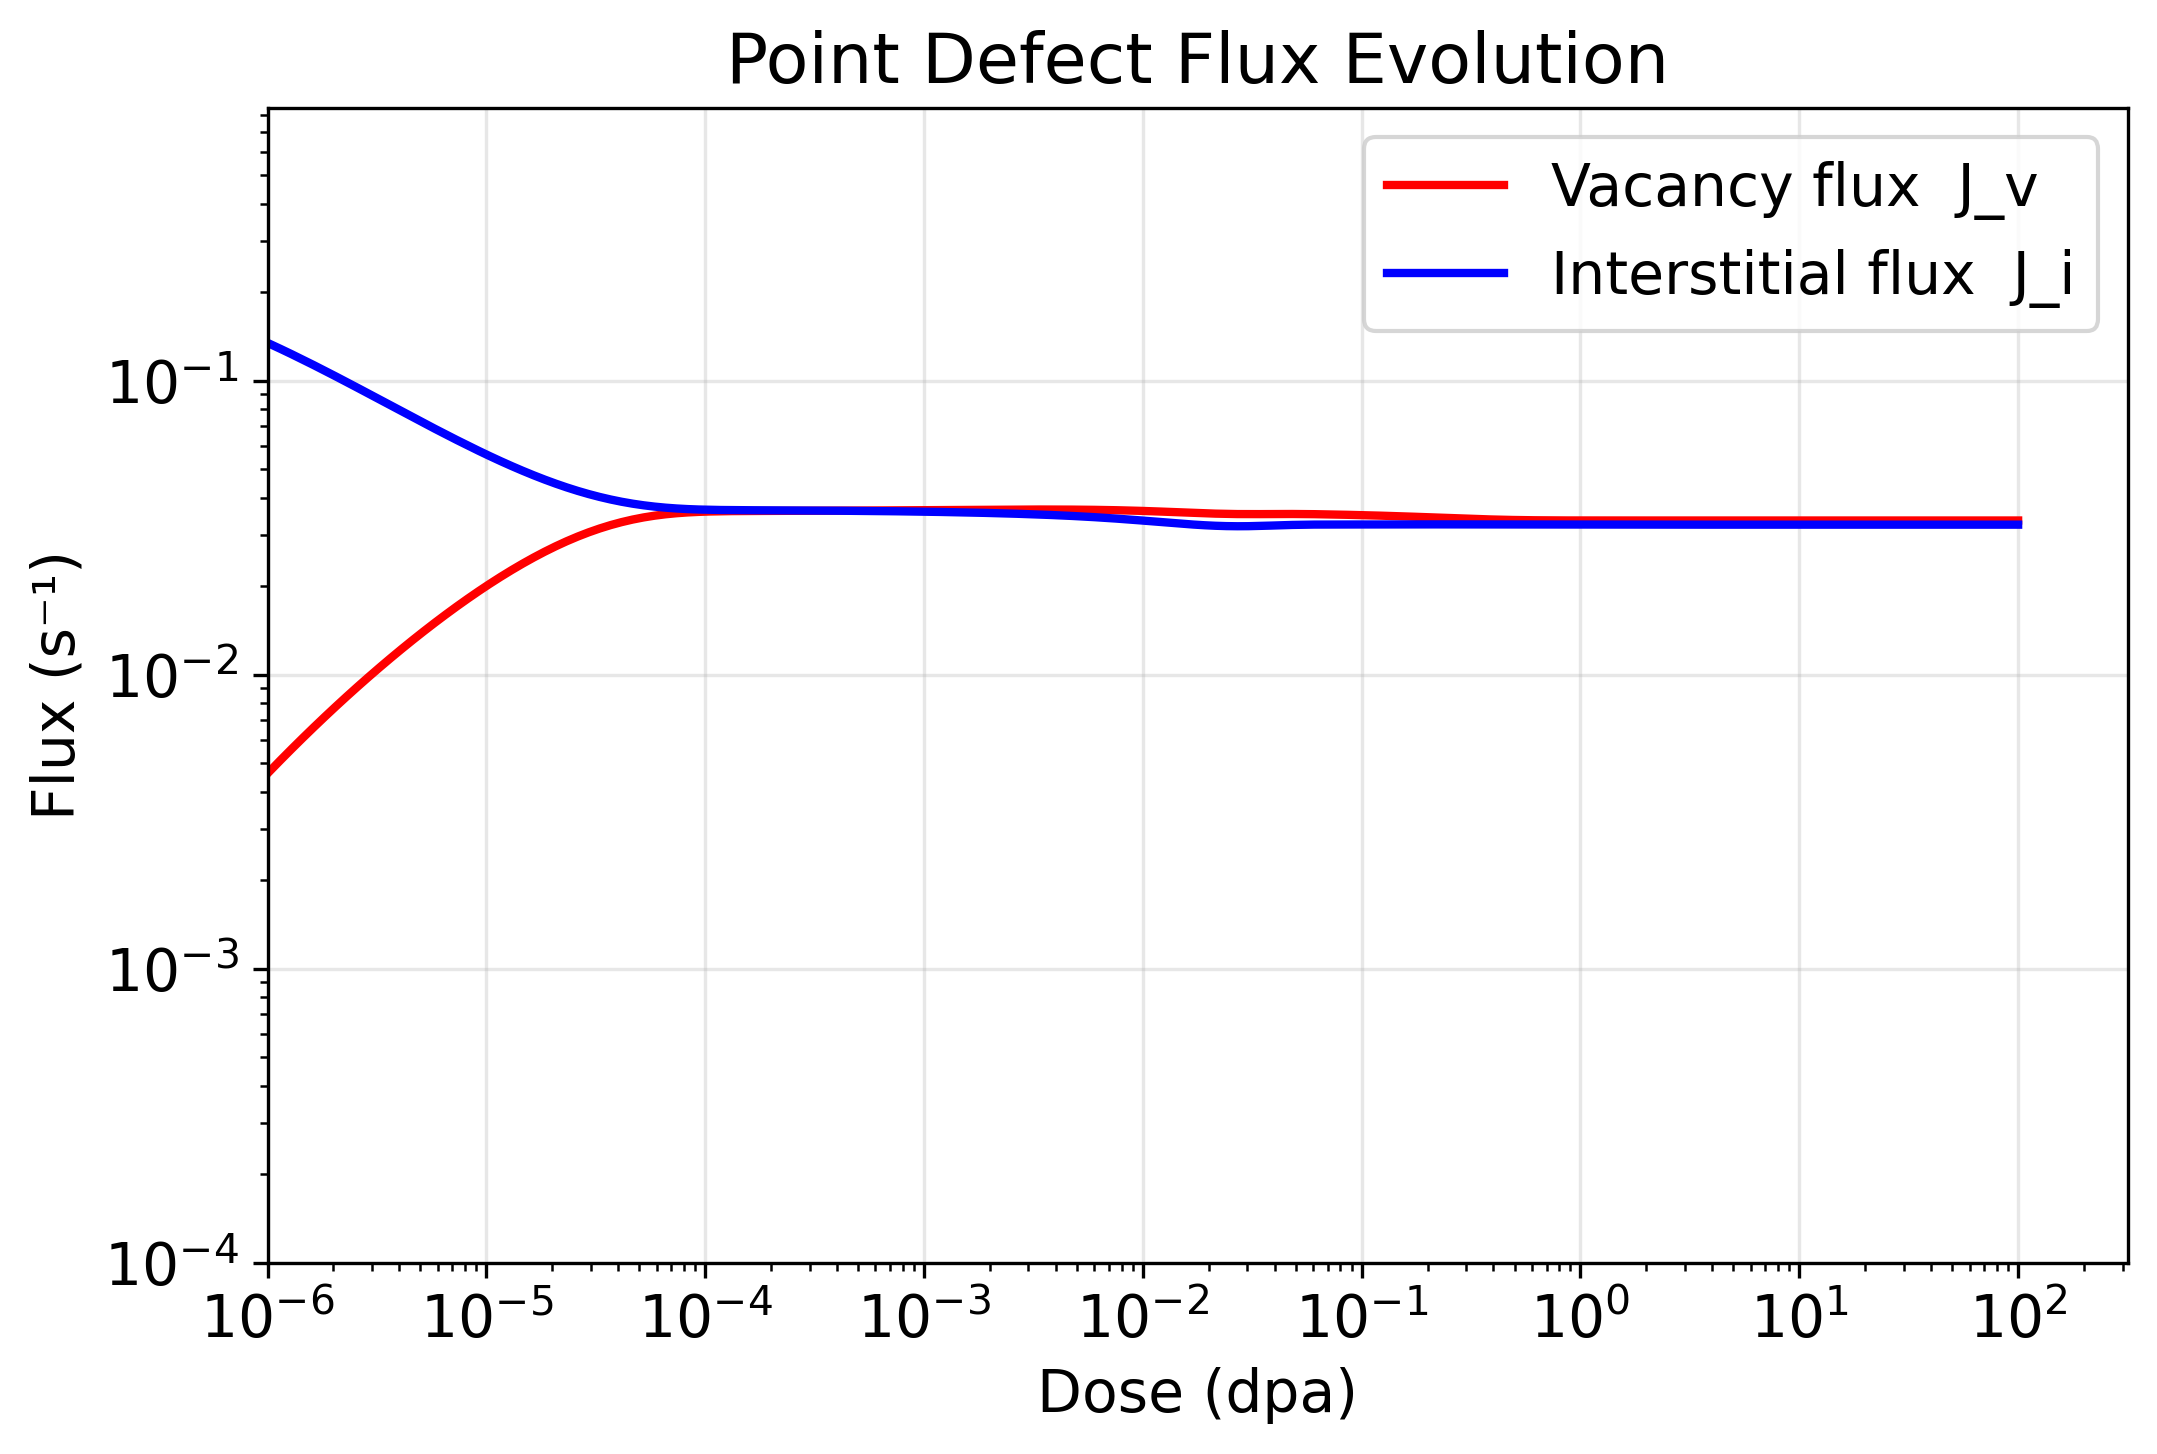
\includegraphics[width=0.49\linewidth]{figures/flux_evolution.png}
\hfill
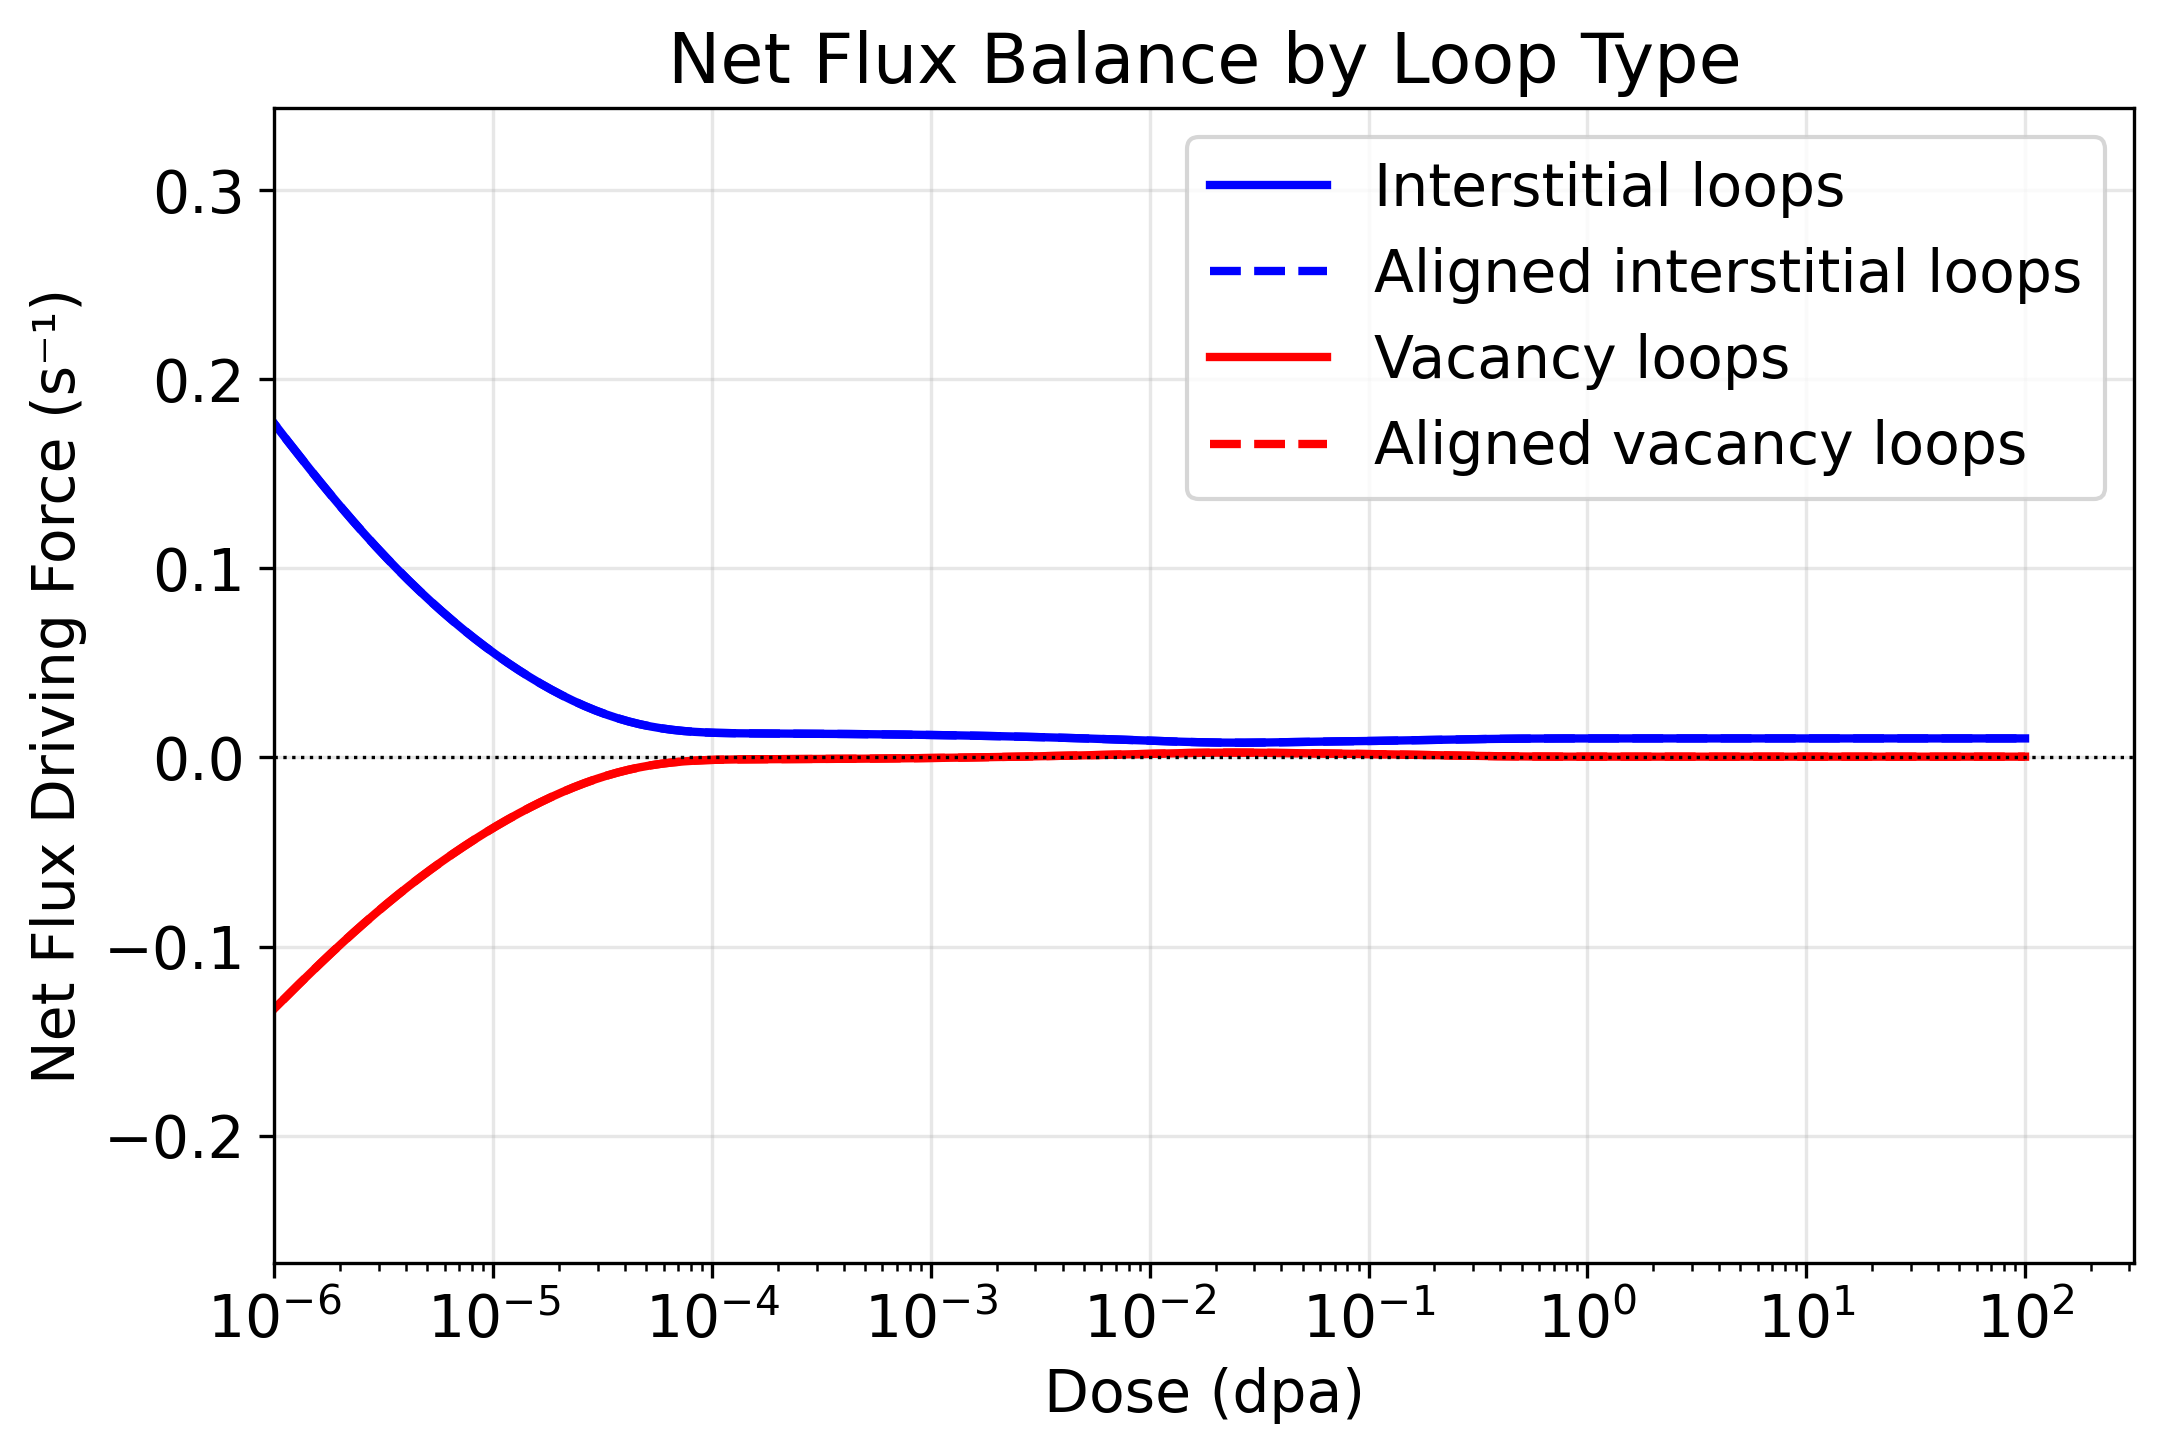
\includegraphics[width=0.49\linewidth]{figures/net_flux_balance.png}
\caption{Defect fluxes to the sinks. Left: the absolute vacancy and interstitial fluxes rise during the transient and saturate together. Right: the small, sign-definite net flux produced by the orientation bias, which controls the growth rate.}
\label{fig:flux_evolution}
\end{figure}

\clearpage
\subsection{Loop microstructure and comparison with Zr data}

The loop densities and sizes are the quantities most directly constrained by the experimental database. Figure~\ref{fig:loop_density} shows that both loop families nucleate between $10^{-5}$ and $10^{-2}\,$dpa, pass through a modest overshoot near $2\times10^{-2}\,$dpa, and saturate—the interstitial ($a$) loops near $4\times10^{21}\,\si{\per\cubic\metre}$ and the vacancy ($c$) loops near $10^{21}\,\si{\per\cubic\metre}$, with the DAD-aligned subsets lying a factor below their parent populations. These plateaux fall within the scatter of the measured $a$-loop densities of Northwood, Jostsons, Kobylyansky, and co-workers, which cluster around $1$--$3\times10^{22}\,\si{\per\cubic\metre}$; the model sits at the lower edge of this band, reflecting the conservative coalescence rate. The companion size plot, Figure~\ref{fig:loop_diameter_vs_dose}, shows the $a$-loop diameter saturating near $9$--$10\,$nm, in good agreement with the bulk of the low- and mid-temperature data, while the $c$-loop (vacancy) diameter climbs after $\sim\!10^{-1}\,$dpa and saturates near $70\,$nm. The measured $c$-loop sizes of Harte ($573\,$K) and Tournadre ($583\,$K) lie at $95$--$150\,$nm, so the model under-predicts the $c$-loop diameter by roughly a factor of $1.5$--$2$; this remains the principal quantitative discrepancy and motivates the targeted $c$-loop refit. Figure~\ref{fig:loop_density_analysis} breaks the saturated population down by family and orientation and confirms that the interstitial loops dominate the number density while the vacancy loops dominate the stored volume, consistent with the anisotropic-bias picture.

\begin{figure}[htbp]
\centering
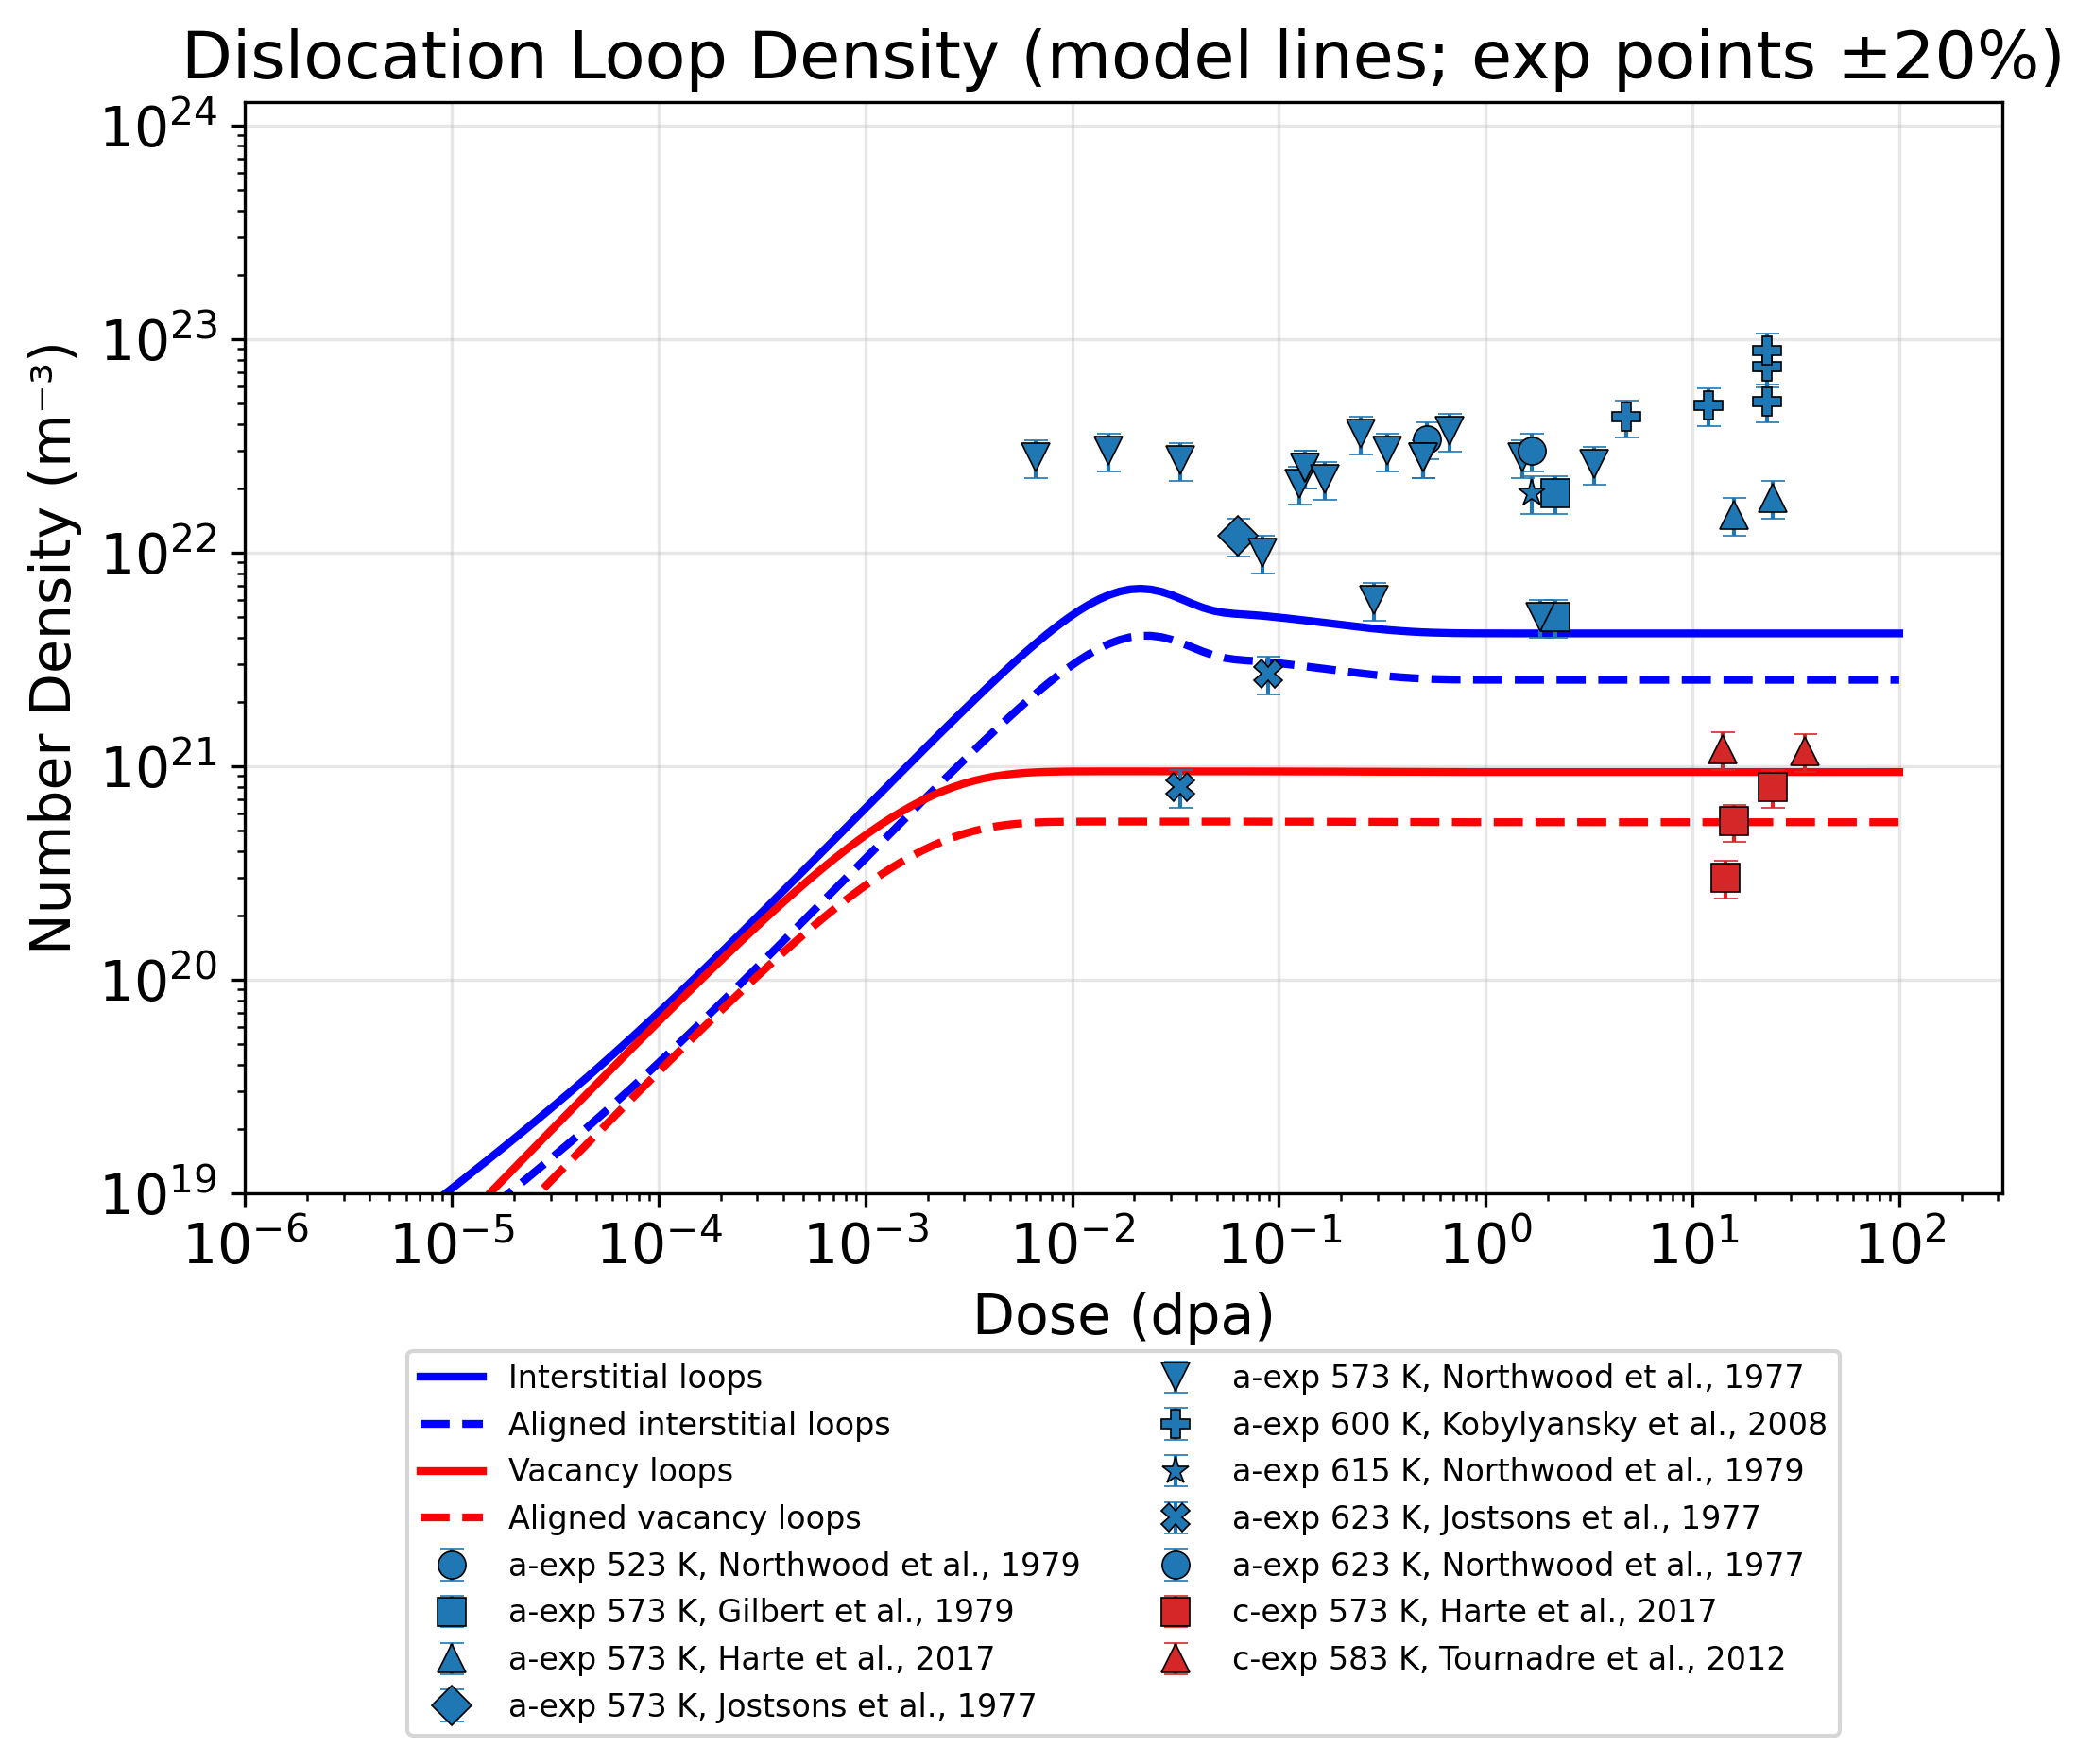
\includegraphics[width=0.7\linewidth]{figures/loop_density.png}
\caption{Dislocation-loop number density versus dose (model lines; experimental points with $\pm20\%$ bars). Interstitial and vacancy loops, each with their DAD-aligned subset, nucleate, overshoot near $2\times10^{-2}\,$dpa, and saturate. The $a$-loop plateau sits at the lower edge of the measured $1$--$3\times10^{22}\,\si{\per\cubic\metre}$ band.}
\label{fig:loop_density}
\end{figure}

\begin{figure}[htbp]
\centering
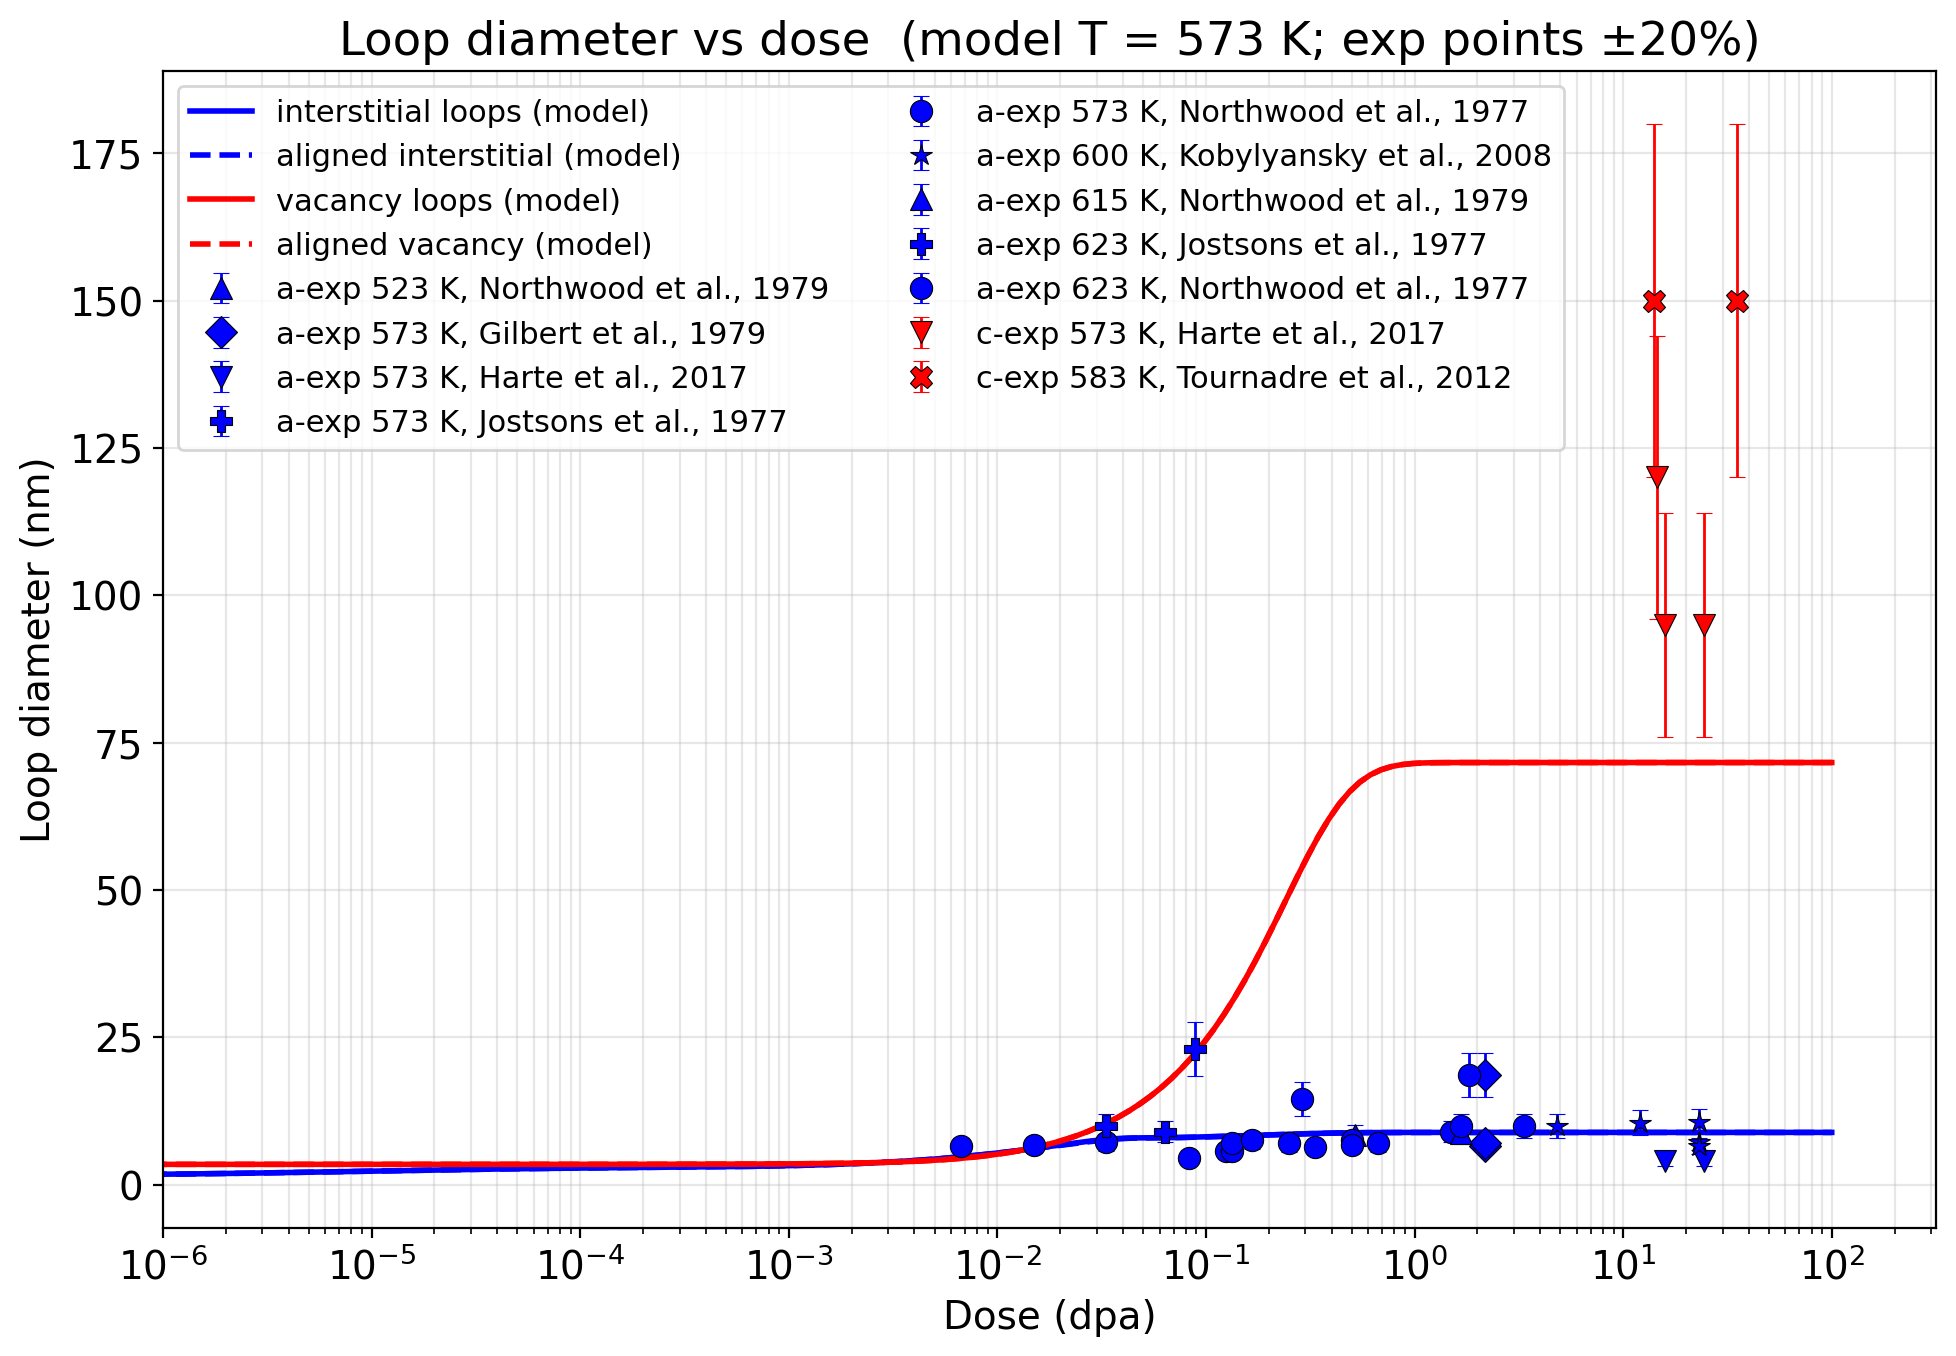
\includegraphics[width=0.7\linewidth]{figures/loop_diameter_vs_dose.png}
\caption{Loop diameter versus dose. The $a$-loop (interstitial) diameter saturates near $9$--$10\,$nm in agreement with the low/mid-$T$ data; the $c$-loop (vacancy) diameter saturates near $70\,$nm, below the measured $95$--$150\,$nm, the main remaining discrepancy.}
\label{fig:loop_diameter_vs_dose}
\end{figure}

\begin{figure}[htbp]
\centering
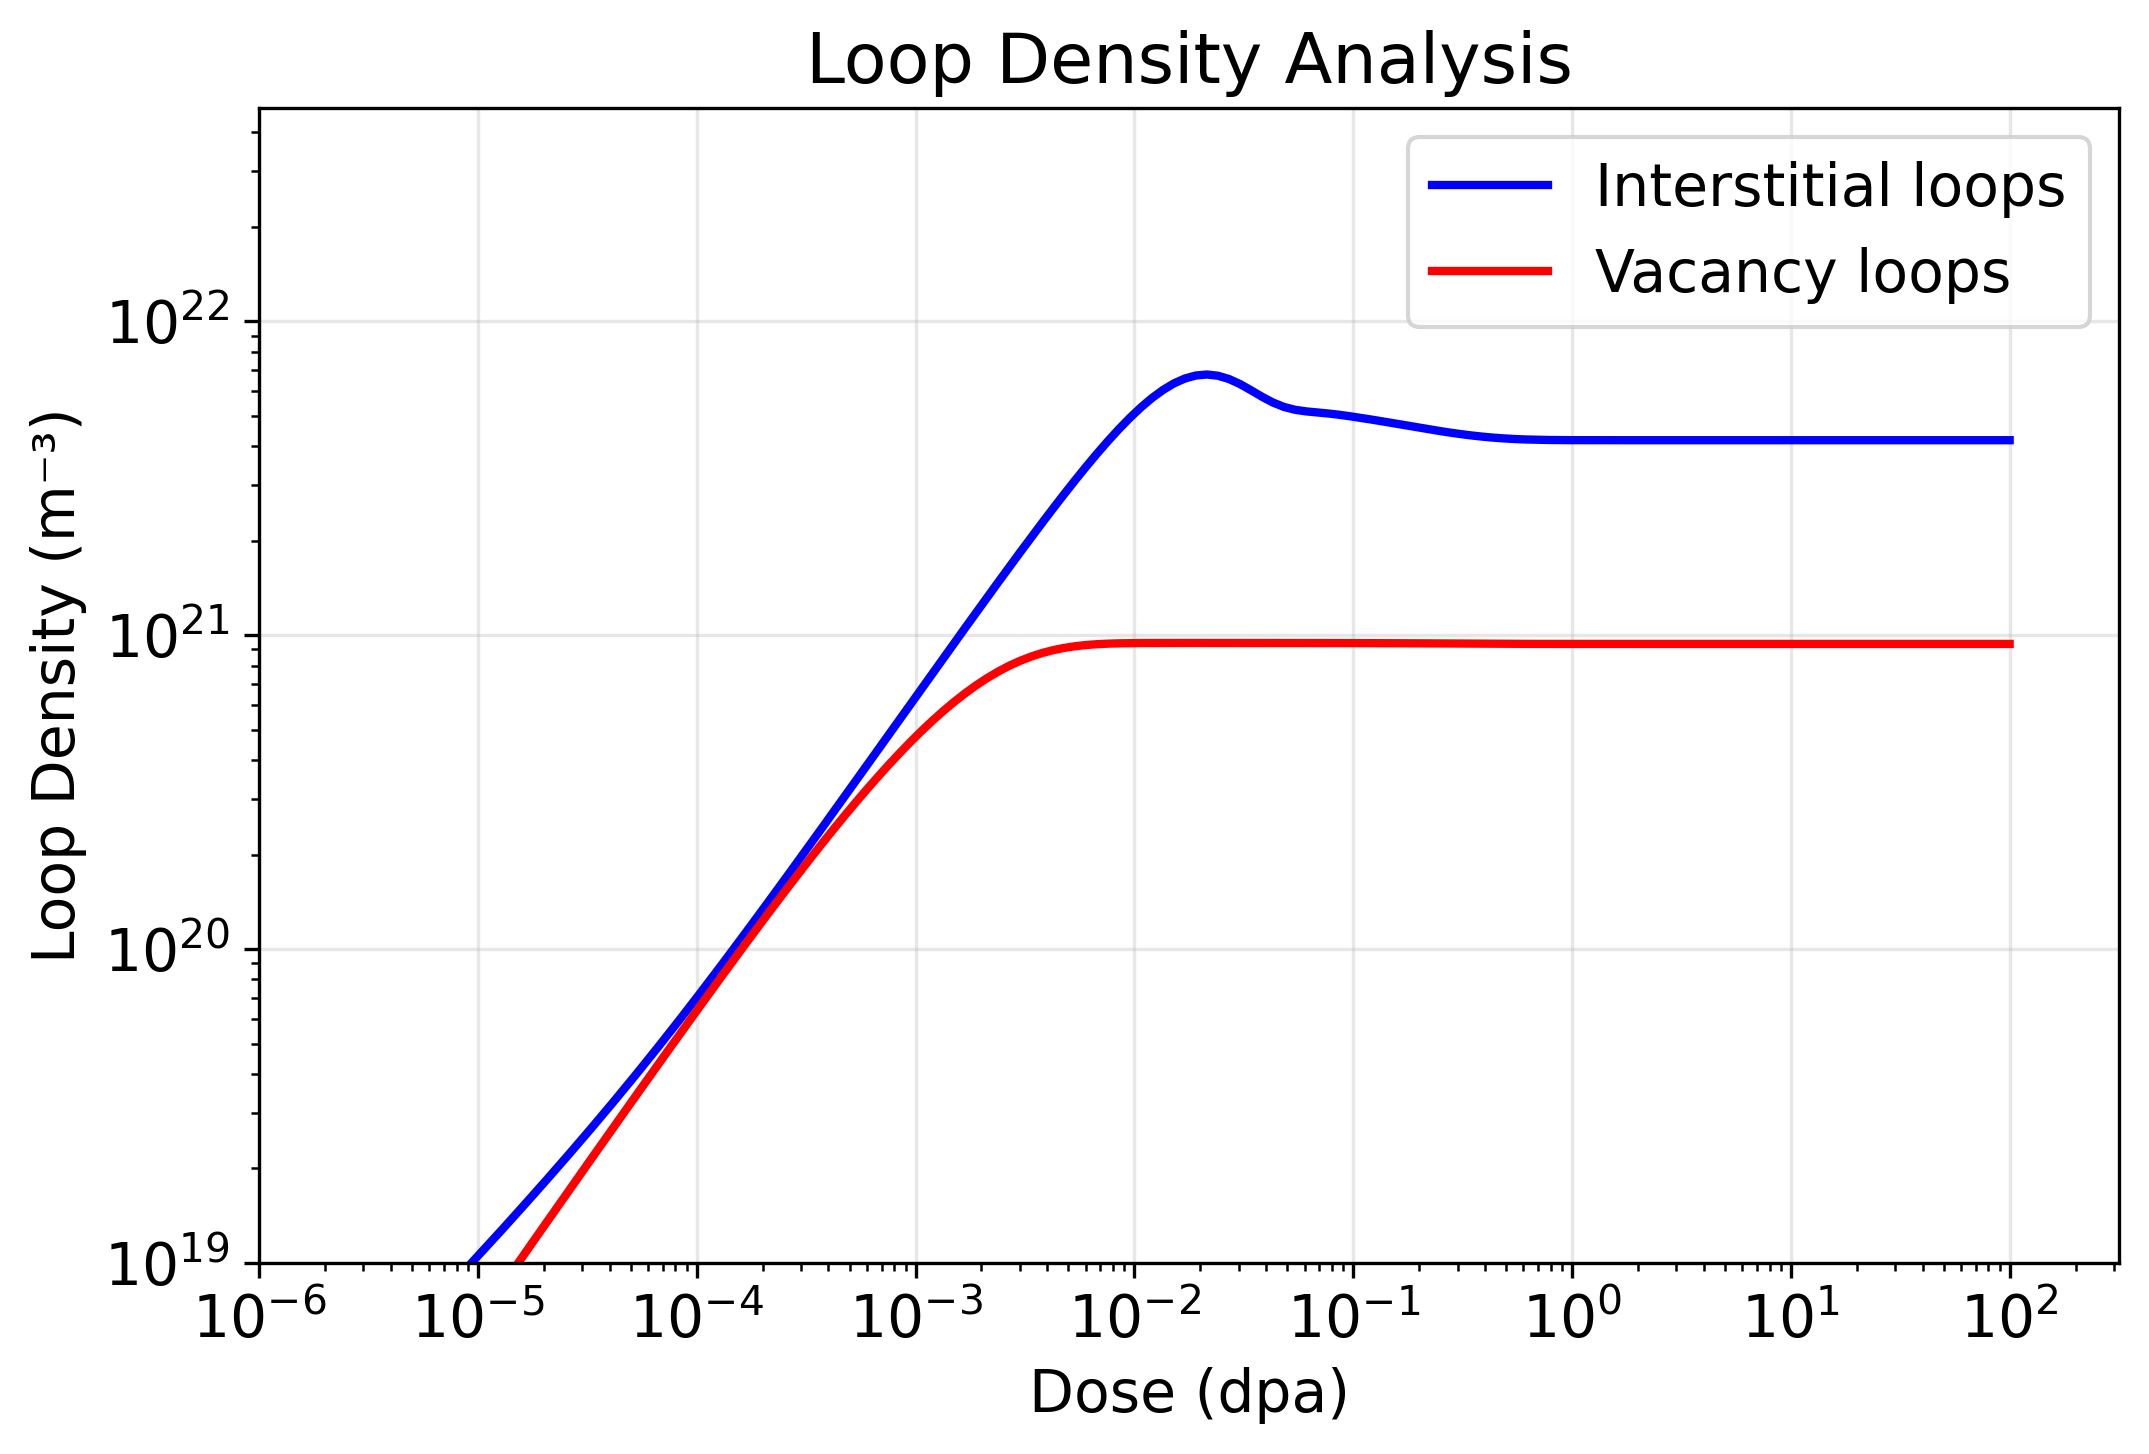
\includegraphics[width=0.7\linewidth]{figures/loop_density_analysis.png}
\caption{Decomposition of the saturated loop population by family and orientation, showing that interstitial loops control the number density while vacancy loops control the stored defect volume.}
\label{fig:loop_density_analysis}
\end{figure}

The temperature-resolved comparisons make the agreement quantitative. Figure~\ref{fig:aloop_density_vs_experiment} overlays the model curves, color-coded by temperature, on the $a$-loop density and diameter measurements between $473$ and $673\,$K. The predicted saturation density decreases monotonically with increasing temperature---from the cold $473\,$K curve down to the hot $668\,$K curve---reproducing the well-known thermal suppression of loop number density through enhanced vacancy mobility and recombination, and the model passes through the bulk of the color-matched data. The $a$-loop diameter saturates near $8$--$11\,$nm at all temperatures, matching the low- and mid-temperature points; the large $30$--$62\,$nm diameters reported at $668$--$673\,$K are the vacancy-character ``$a$'' loops that are deliberately excluded from the interstitial fit and therefore lie above the model line. Figure~\ref{fig:cloop_density_vs_experiment} presents the corresponding $c$-loop comparison: the predicted $c$-loop density saturates near $1.3\times10^{21}\,\si{\per\cubic\metre}$, matching Tournadre ($583\,$K) and bracketing the Harte ($573\,$K) points, whereas the $c$-loop diameter again falls short of the measured values, consistent with the dose-resolved view above.

\begin{figure}[htbp]
\centering
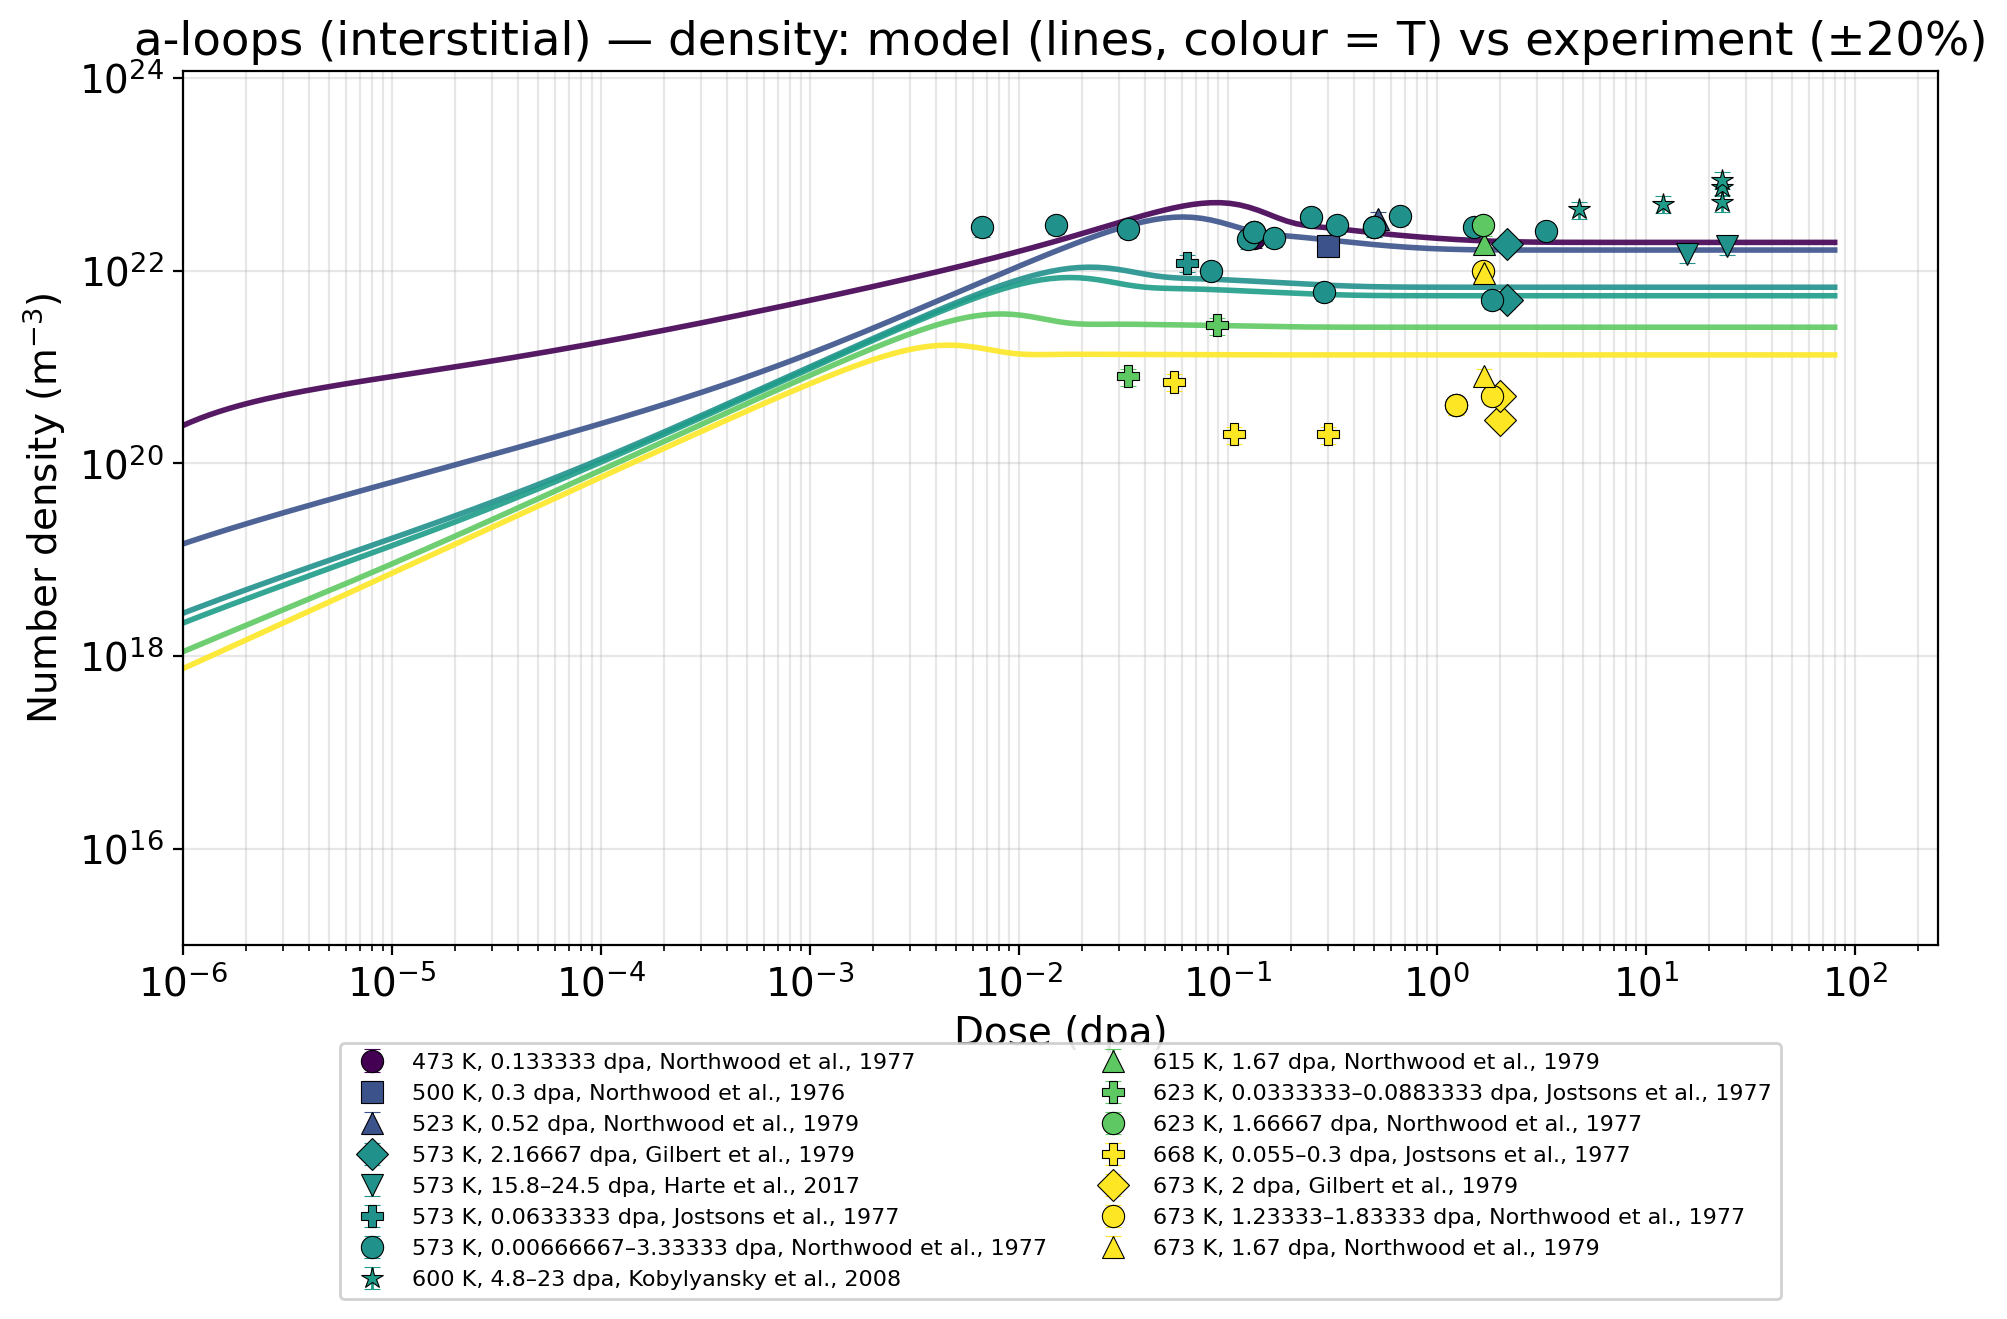
\includegraphics[width=0.49\linewidth]{figures/aloop_density_vs_experiment.png}
\hfill
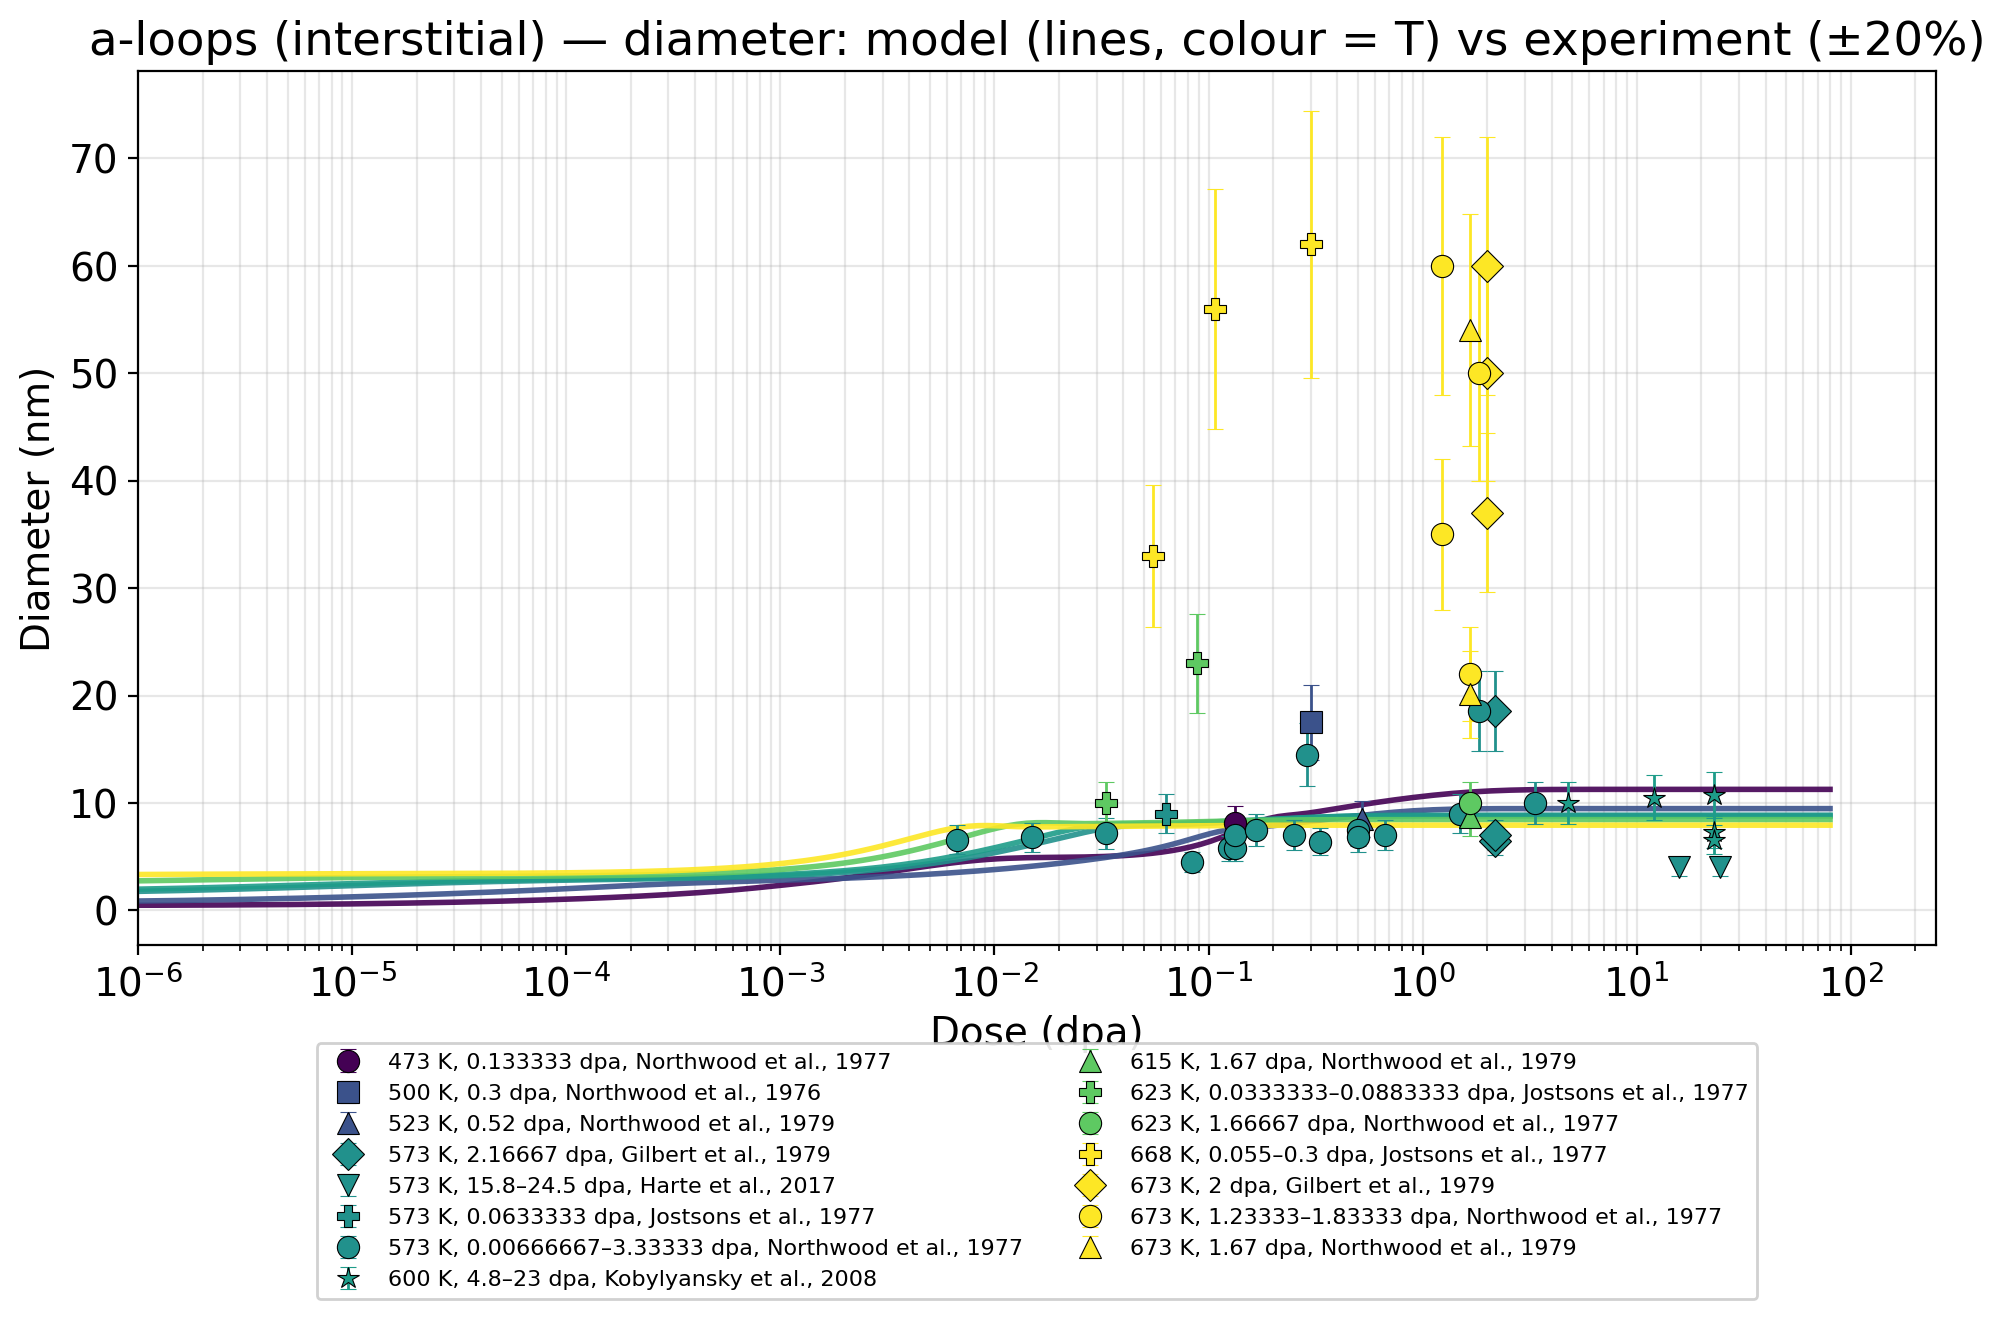
\includegraphics[width=0.49\linewidth]{figures/aloop_diameter_vs_experiment.png}
\caption{Interstitial ($a$) loops versus the temperature-resolved database. Left: number density; the saturation level falls with increasing temperature, tracking the measured thermal suppression. Right: diameter, saturating near $8$--$11\,$nm; the large high-$T$ points are excluded vacancy-character loops.}
\label{fig:aloop_density_vs_experiment}
\end{figure}

\begin{figure}[htbp]
\centering
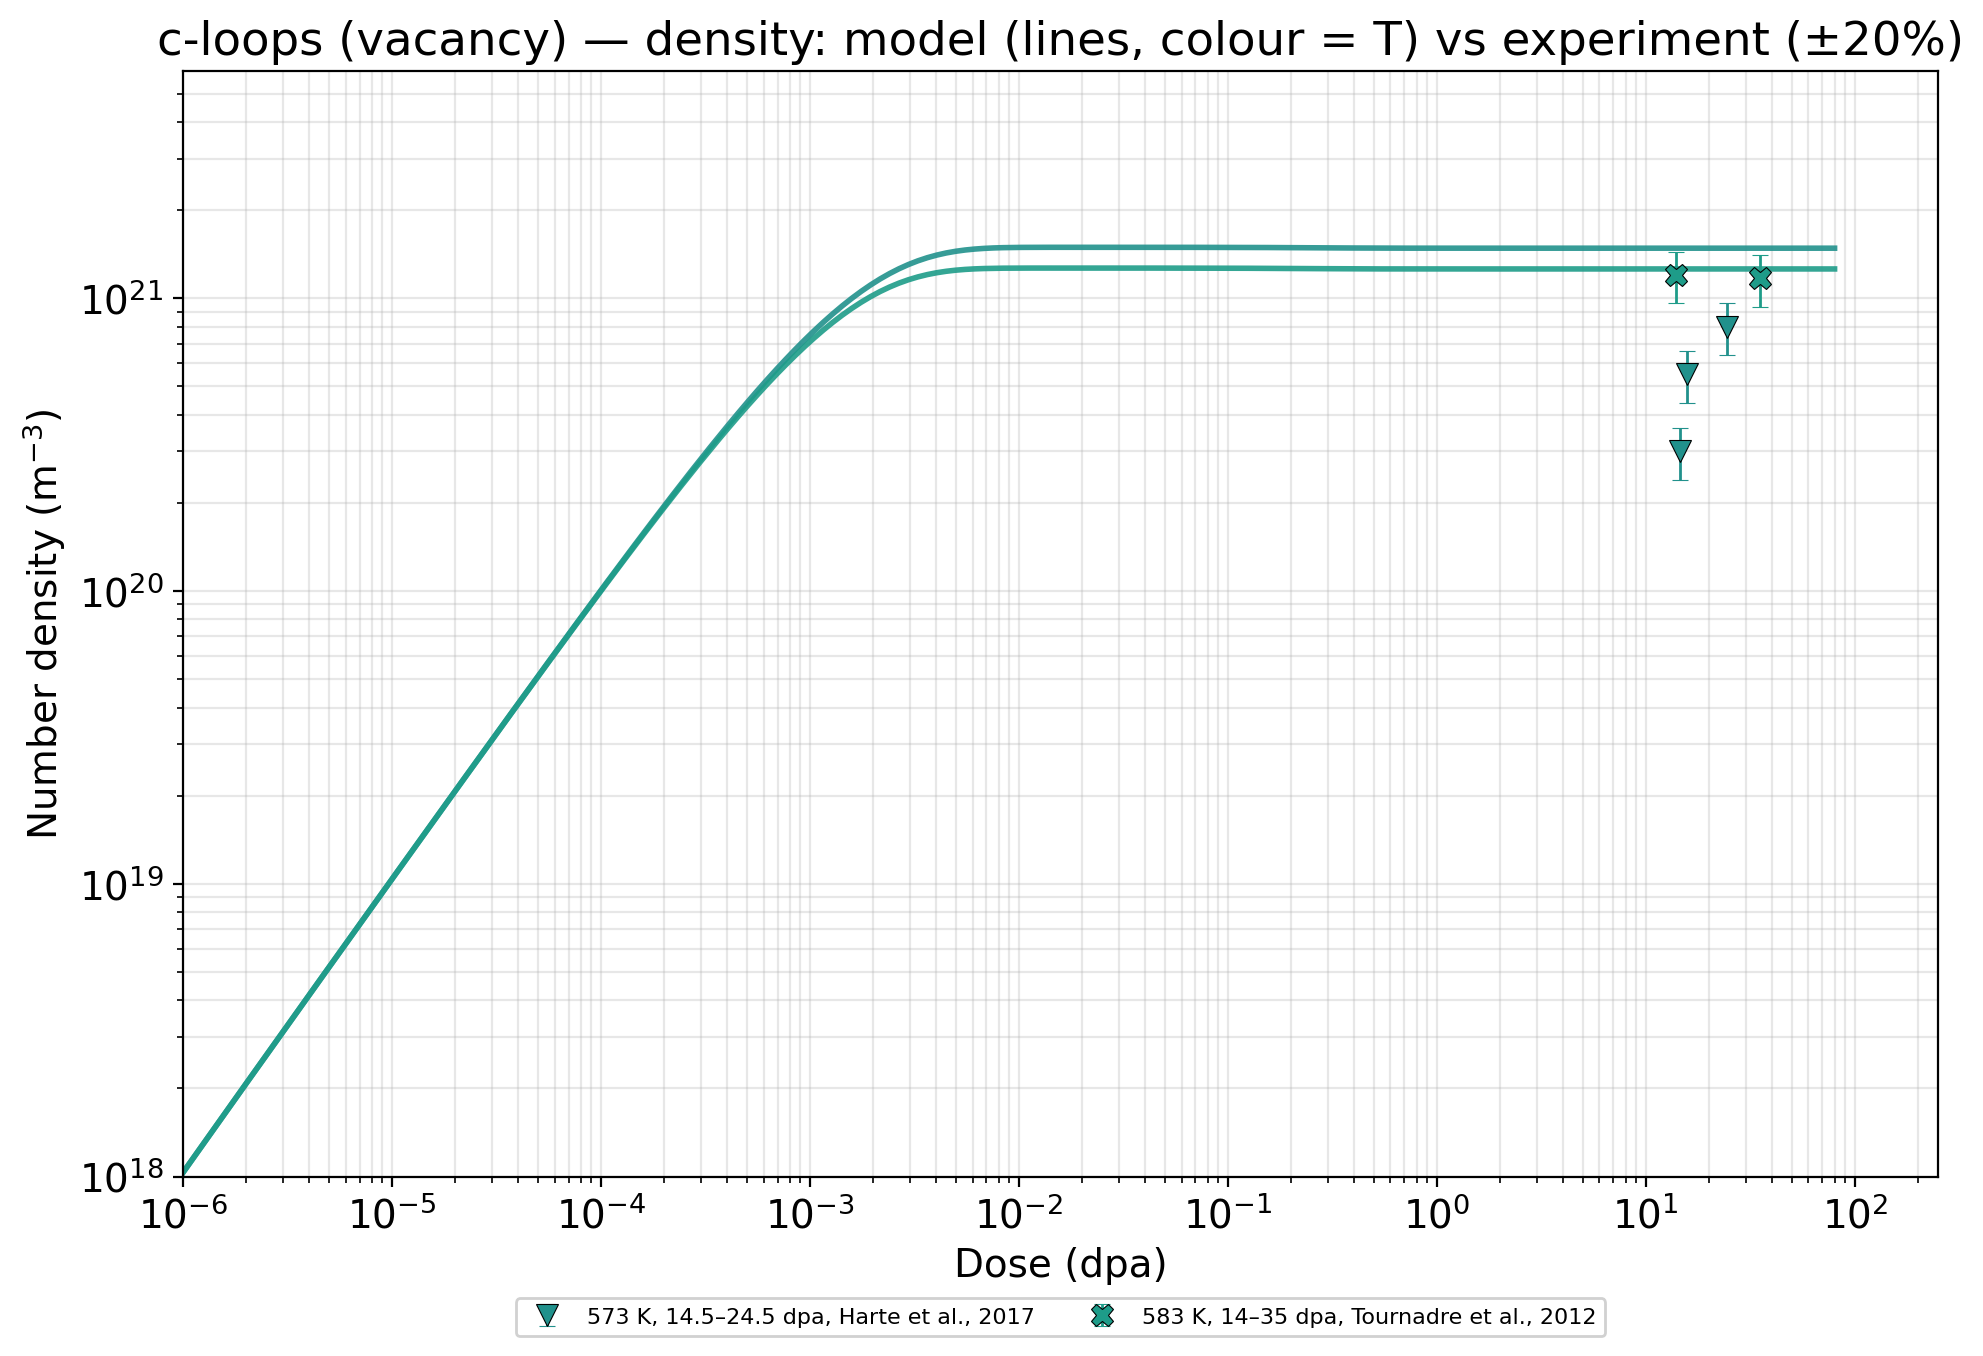
\includegraphics[width=0.49\linewidth]{figures/cloop_density_vs_experiment.png}
\hfill
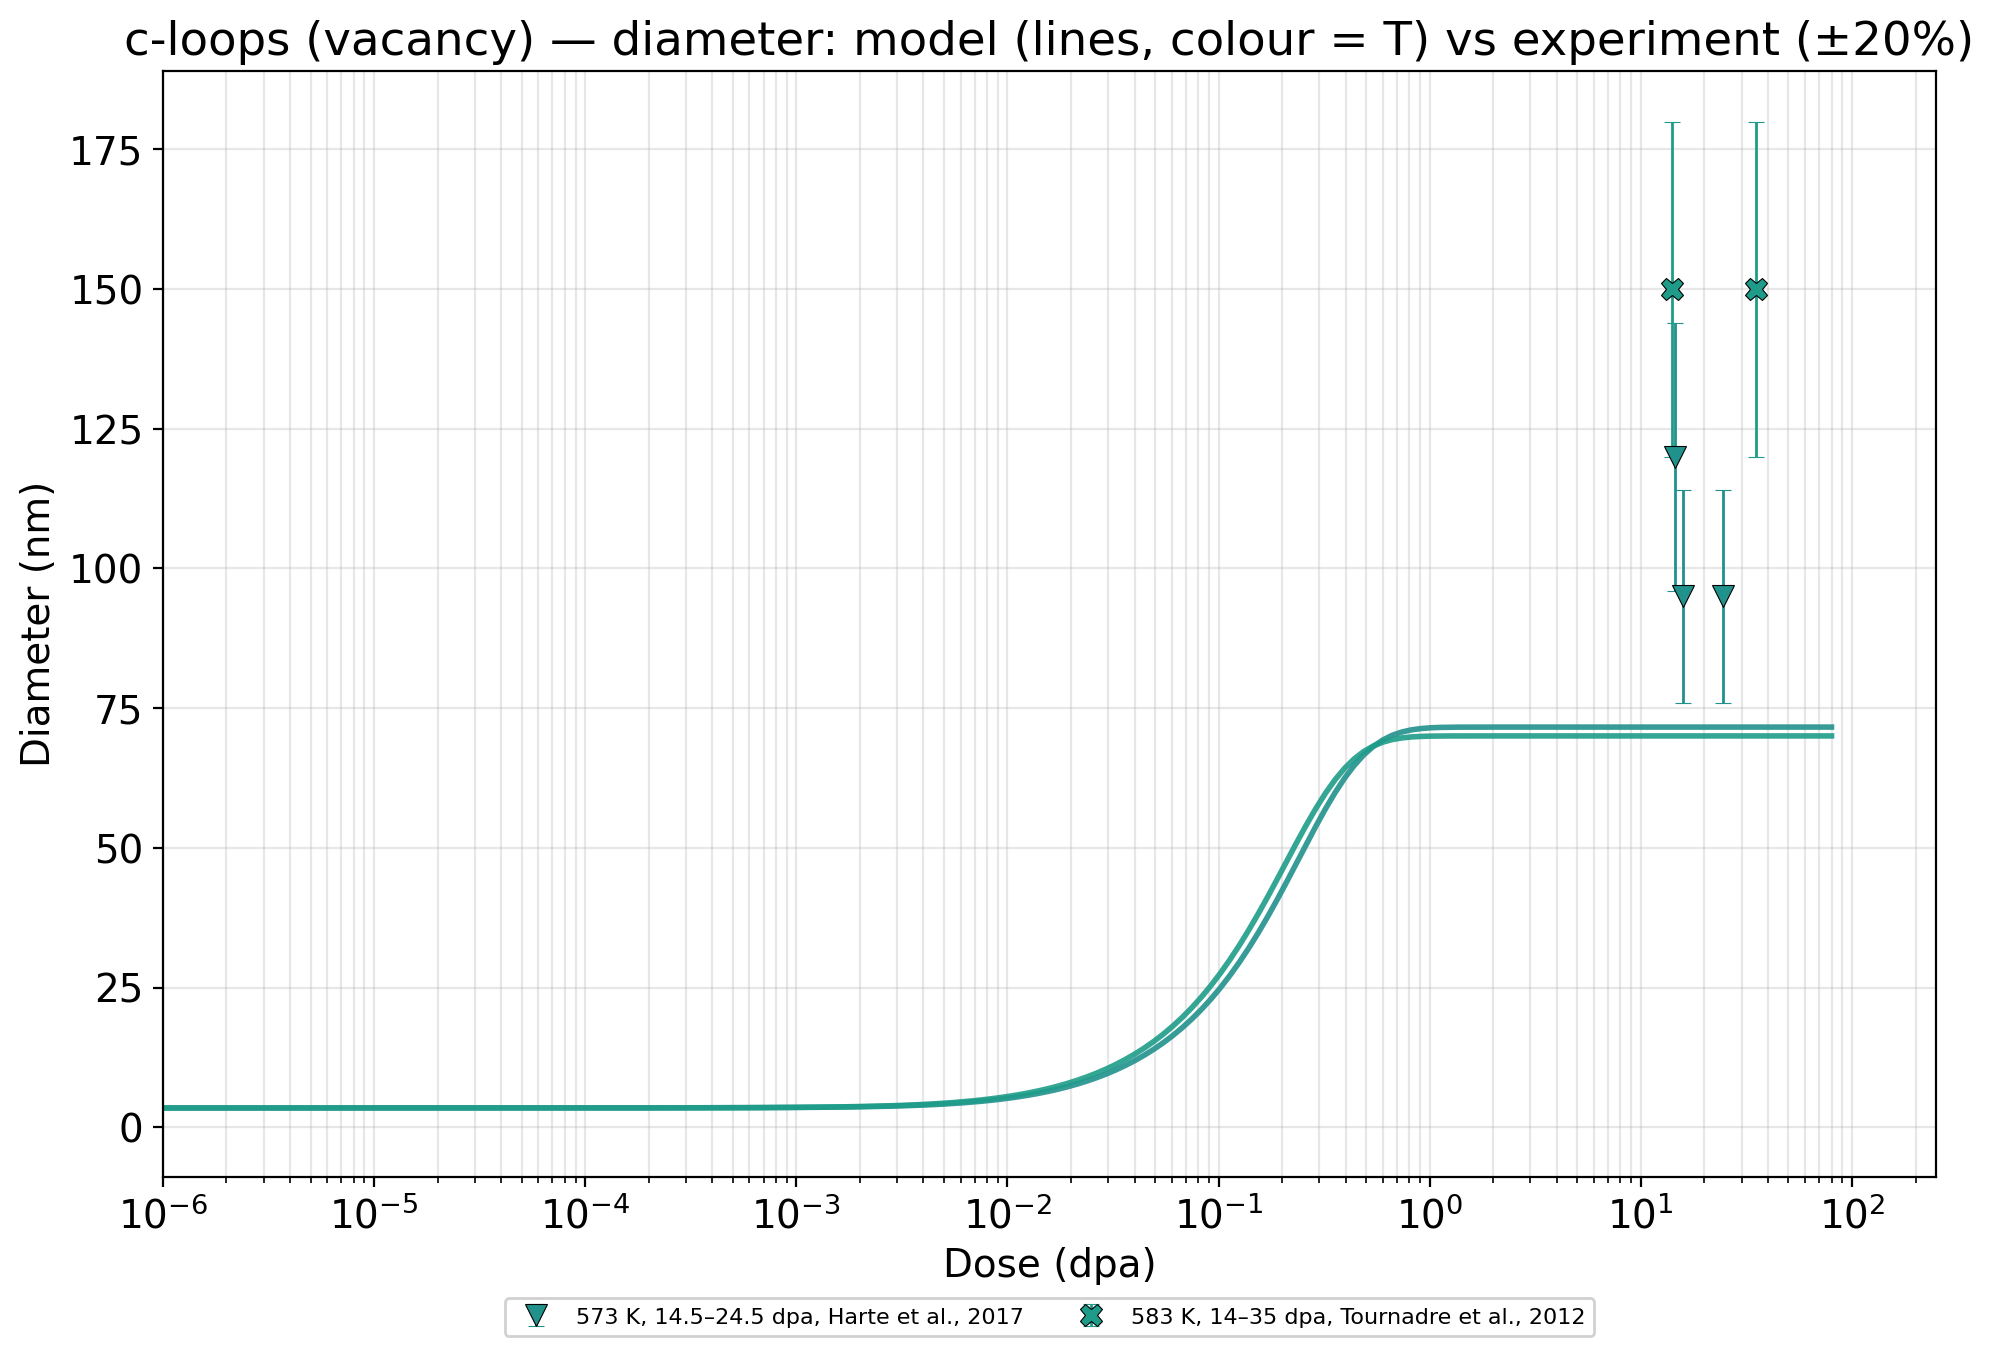
\includegraphics[width=0.49\linewidth]{figures/cloop_diameter_vs_experiment.png}
\caption{Vacancy ($c$) loops versus experiment. Left: the density saturates near $1.3\times10^{21}\,\si{\per\cubic\metre}$, matching Tournadre and bracketing Harte. Right: the diameter saturates below the measured $95$--$150\,$nm, the main residual discrepancy.}
\label{fig:cloop_density_vs_experiment}
\end{figure}

\subsection{Network evolution, sink spacing, and conservation checks}

The evolving network dislocation density and the geometric spacing of the sinks complete the microstructural description. Figure~\ref{fig:network_density_evolution} shows $\rho_N$ relaxing from its grown-in seed and saturating, having absorbed loops that unfault and join the network while coalescence limits further growth; this saturating network is what closes the sink-strength balance at high doses. Figure~\ref{fig:loop_network_spacing} shows the mean loop-to-network and loop-to-loop spacings, both of which decrease as the loop density builds and then level off at the inter-obstacle distance that sets the hardening and the coalescence rate; their saturation is the geometric counterpart of the density plateau in Figure~\ref{fig:loop_density}.

\begin{figure}[htbp]
\centering
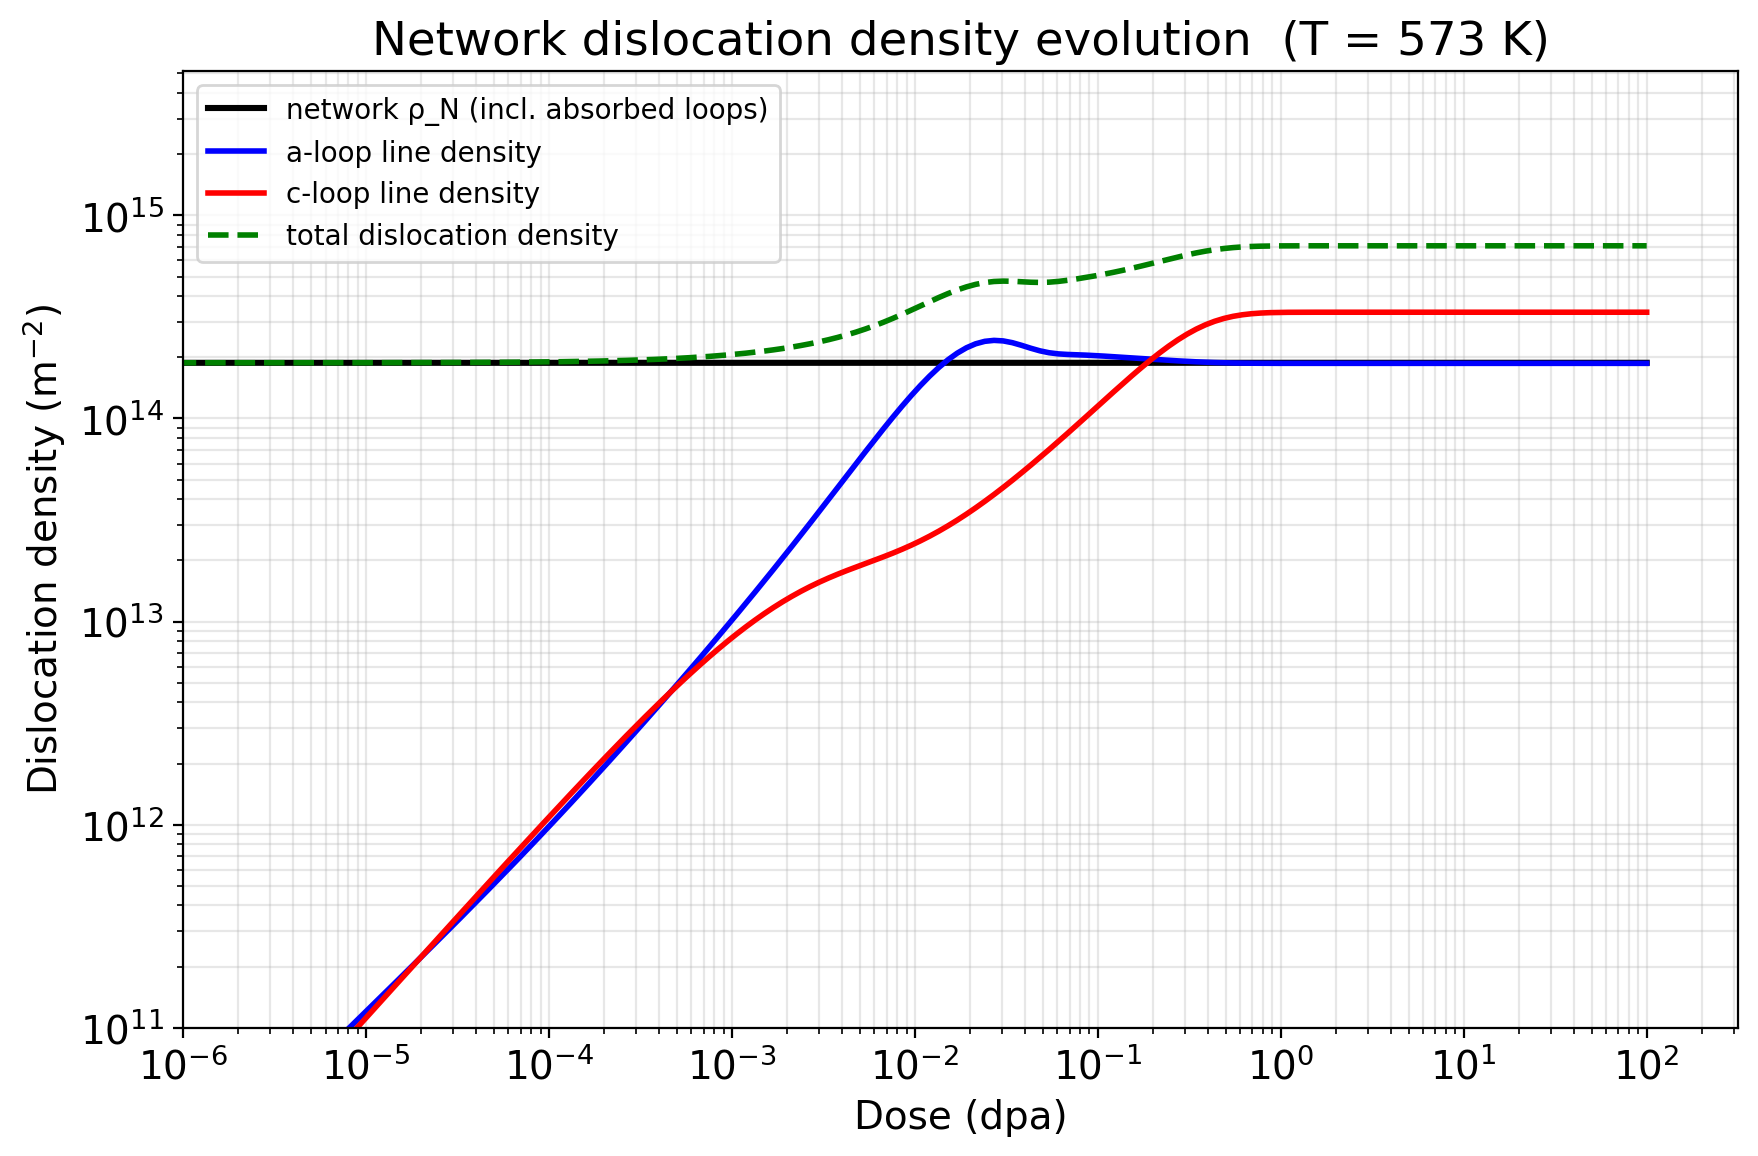
\includegraphics[width=0.7\linewidth]{figures/network_density_evolution.png}
\caption{Evolution of the network dislocation density $\rho_N$, which relaxes from its grown-in seed and saturates as unfaulted loops feed the network and coalescence limits further growth.}
\label{fig:network_density_evolution}
\end{figure}

\begin{figure}[htbp]
\centering
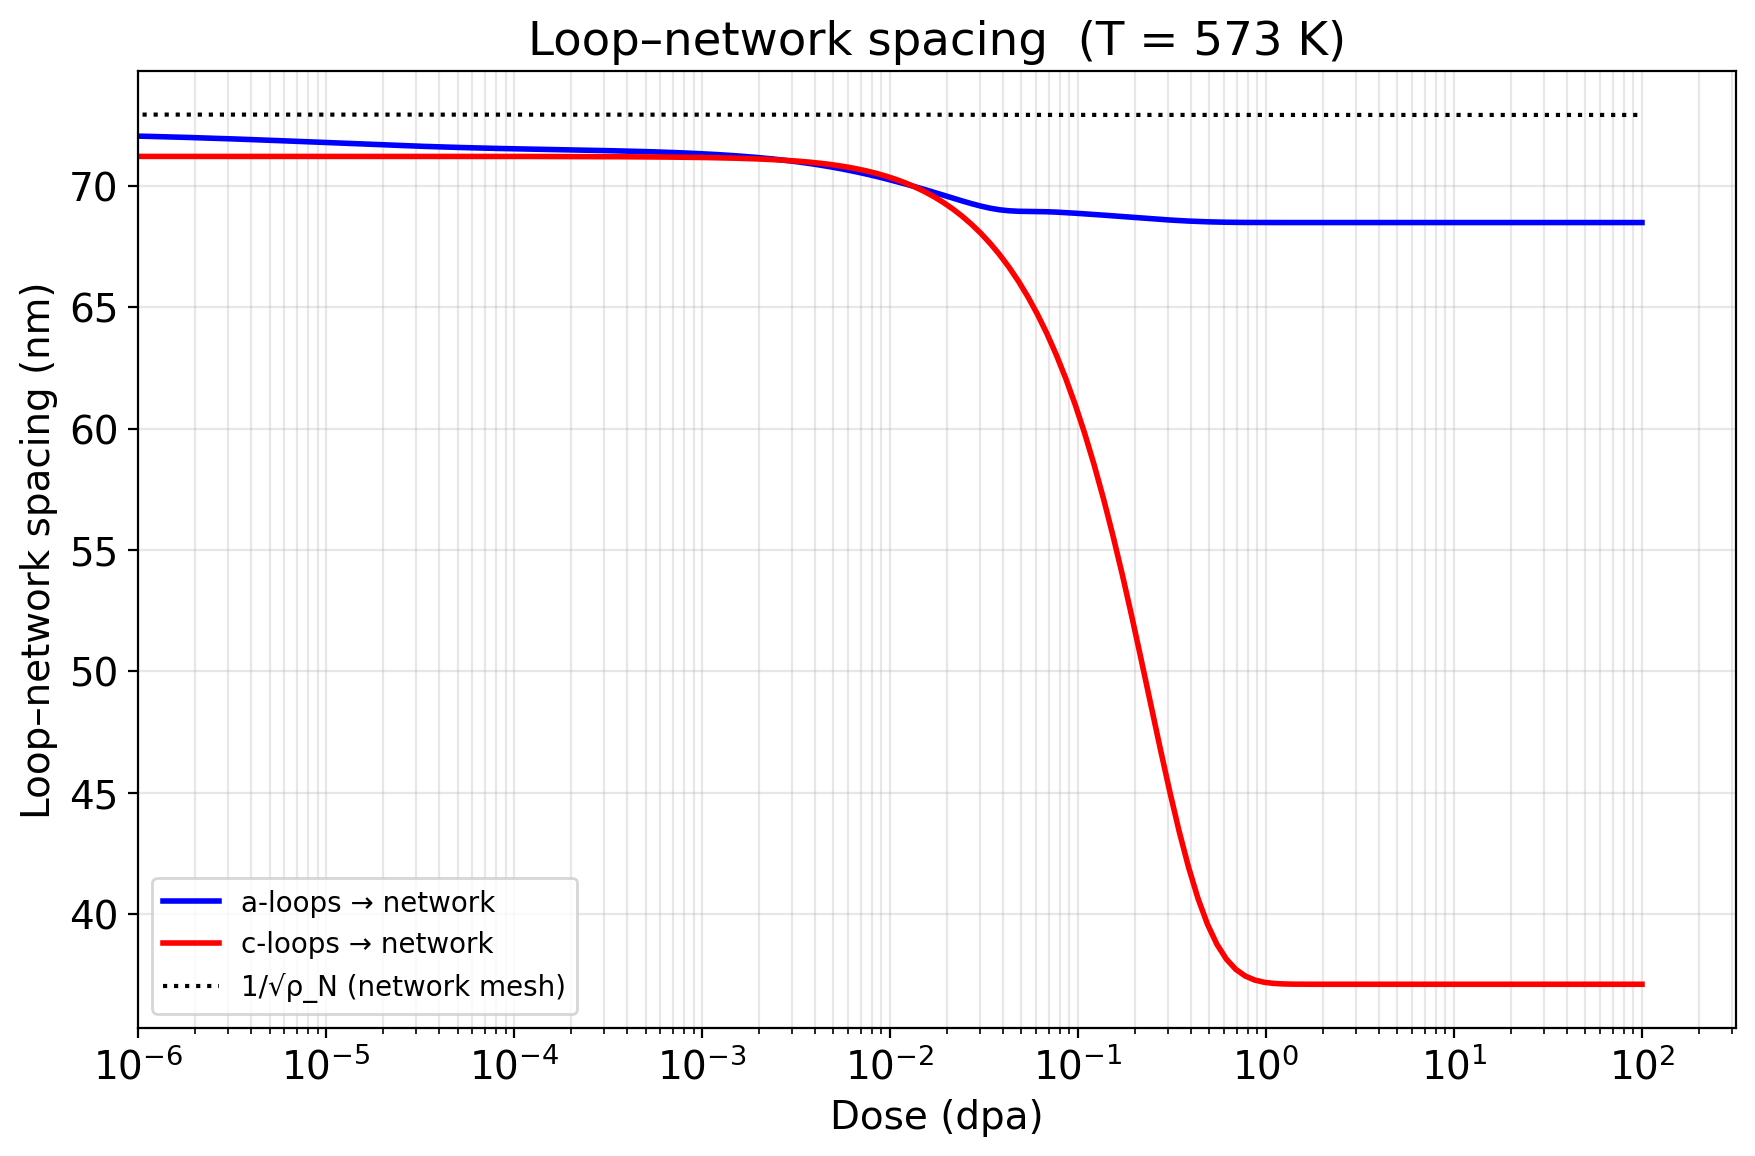
\includegraphics[width=0.49\linewidth]{figures/loop_network_spacing.png}
\hfill
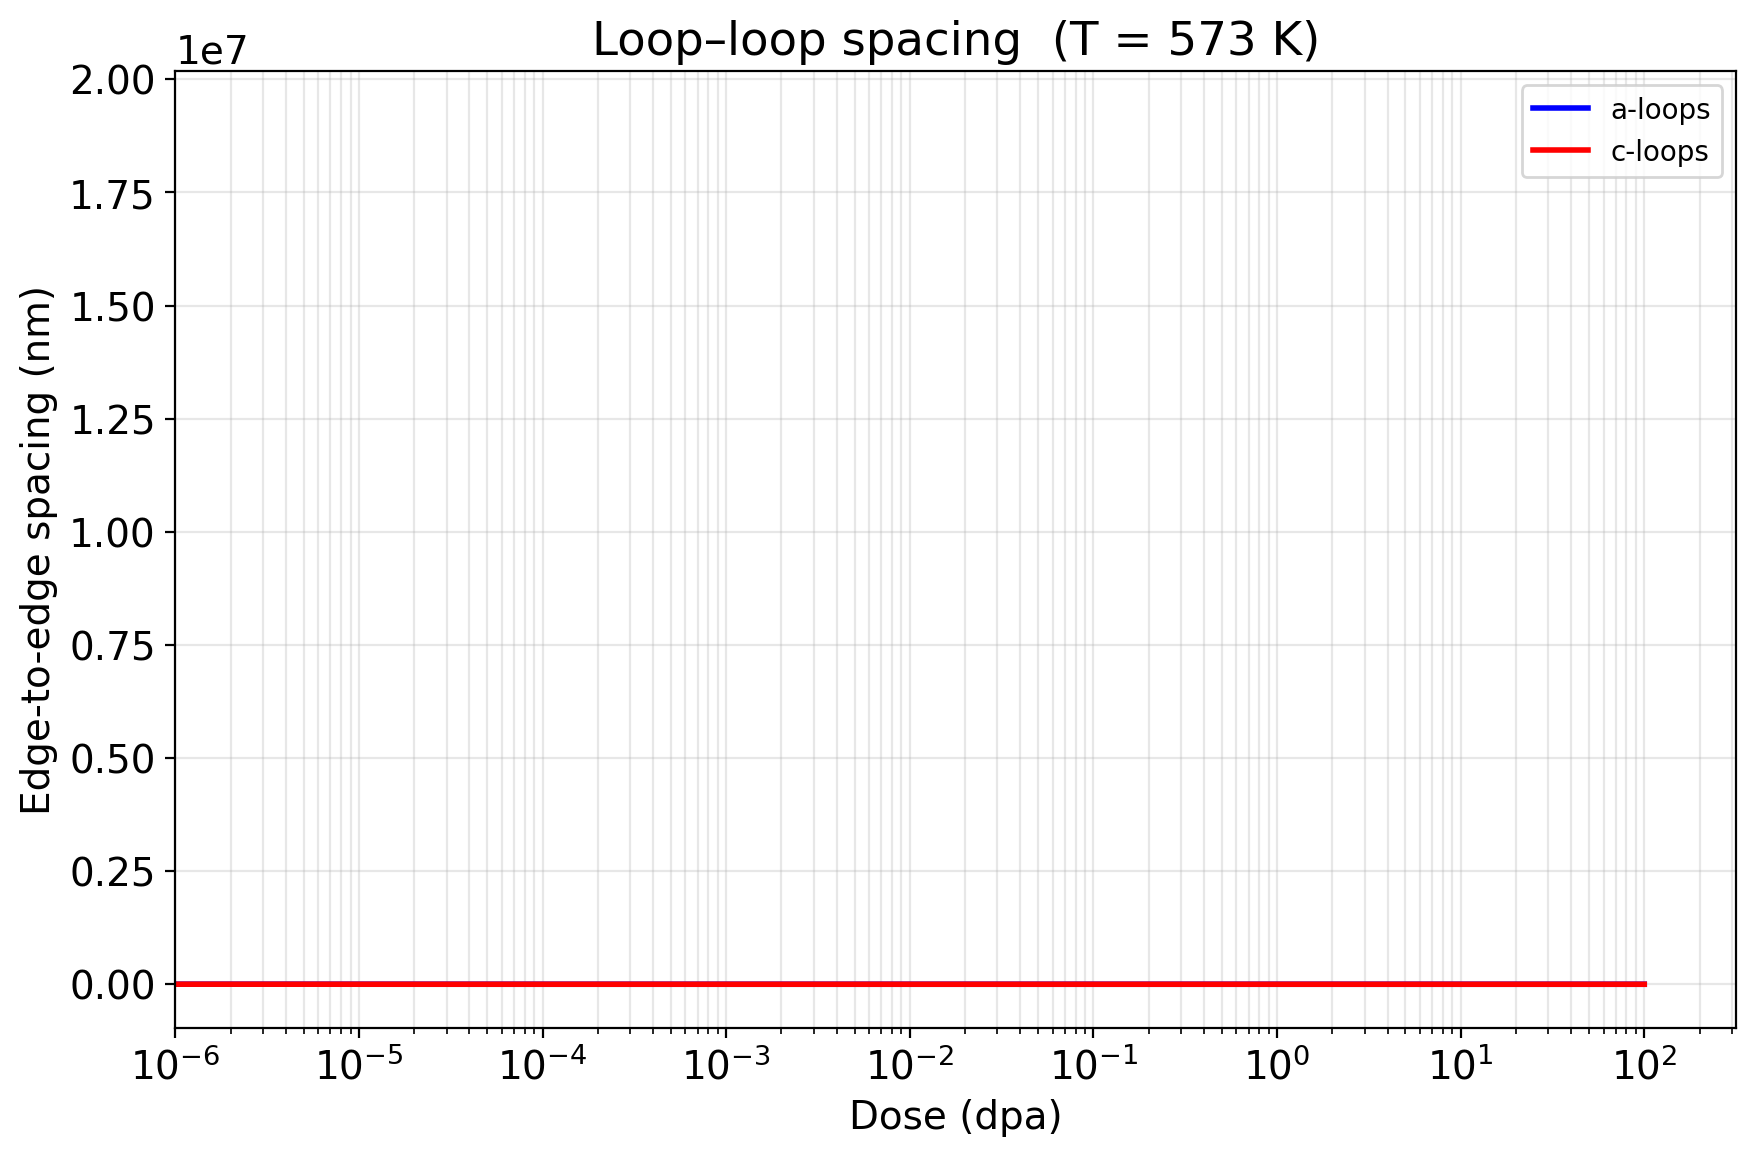
\includegraphics[width=0.49\linewidth]{figures/loop_loop_spacing.png}
\caption{Mean loop-to-network (left) and loop-to-loop (right) spacings. Both contract as the loop density builds and saturate at the inter-obstacle distance that governs hardening and coalescence.}
\label{fig:loop_network_spacing}
\end{figure}

Finally, the conservation diagnostics verify that these results are numerically trustworthy. Figure~\ref{fig:conservation_channels_i} decomposes the interstitial and vacancy budgets into their production, recombination, and absorption channels, and shows that production is balanced by the sum of the sink channels at every dose. Figure~\ref{fig:conservation_error} reports the running relative error in the global defect balance, which remains at the round-off level throughout the integration, confirming that the build-up, overshoot, and saturation features above are physical and not numerical artifacts.

\begin{figure}[htbp]
\centering
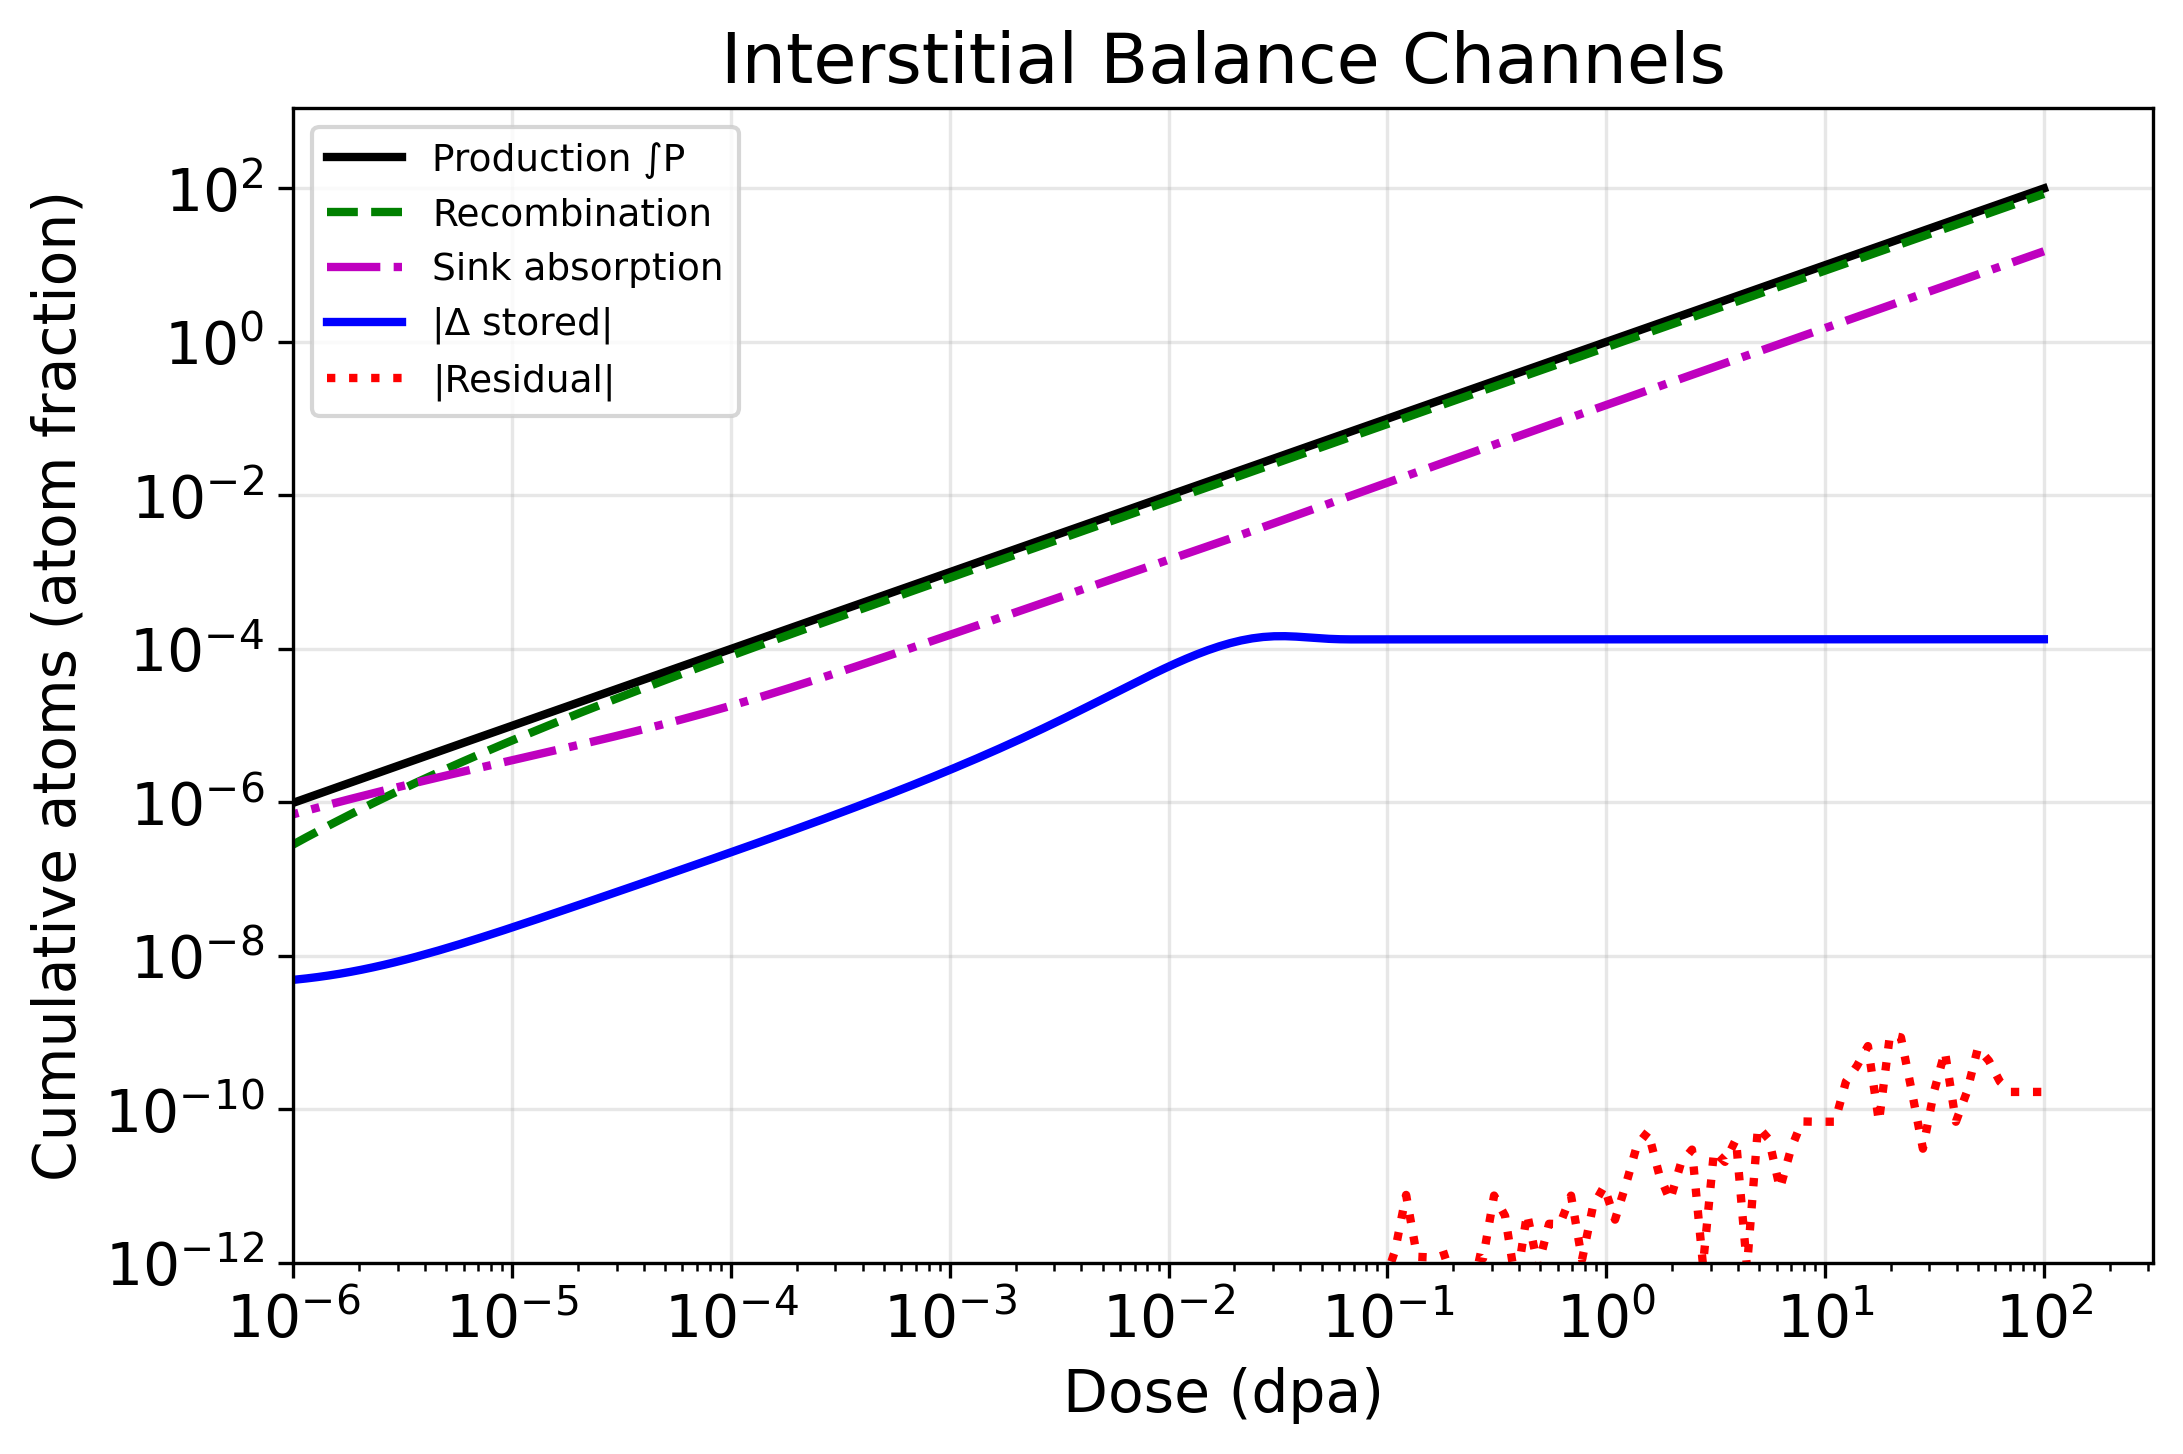
\includegraphics[width=0.49\linewidth]{figures/conservation_channels_i.png}
\hfill
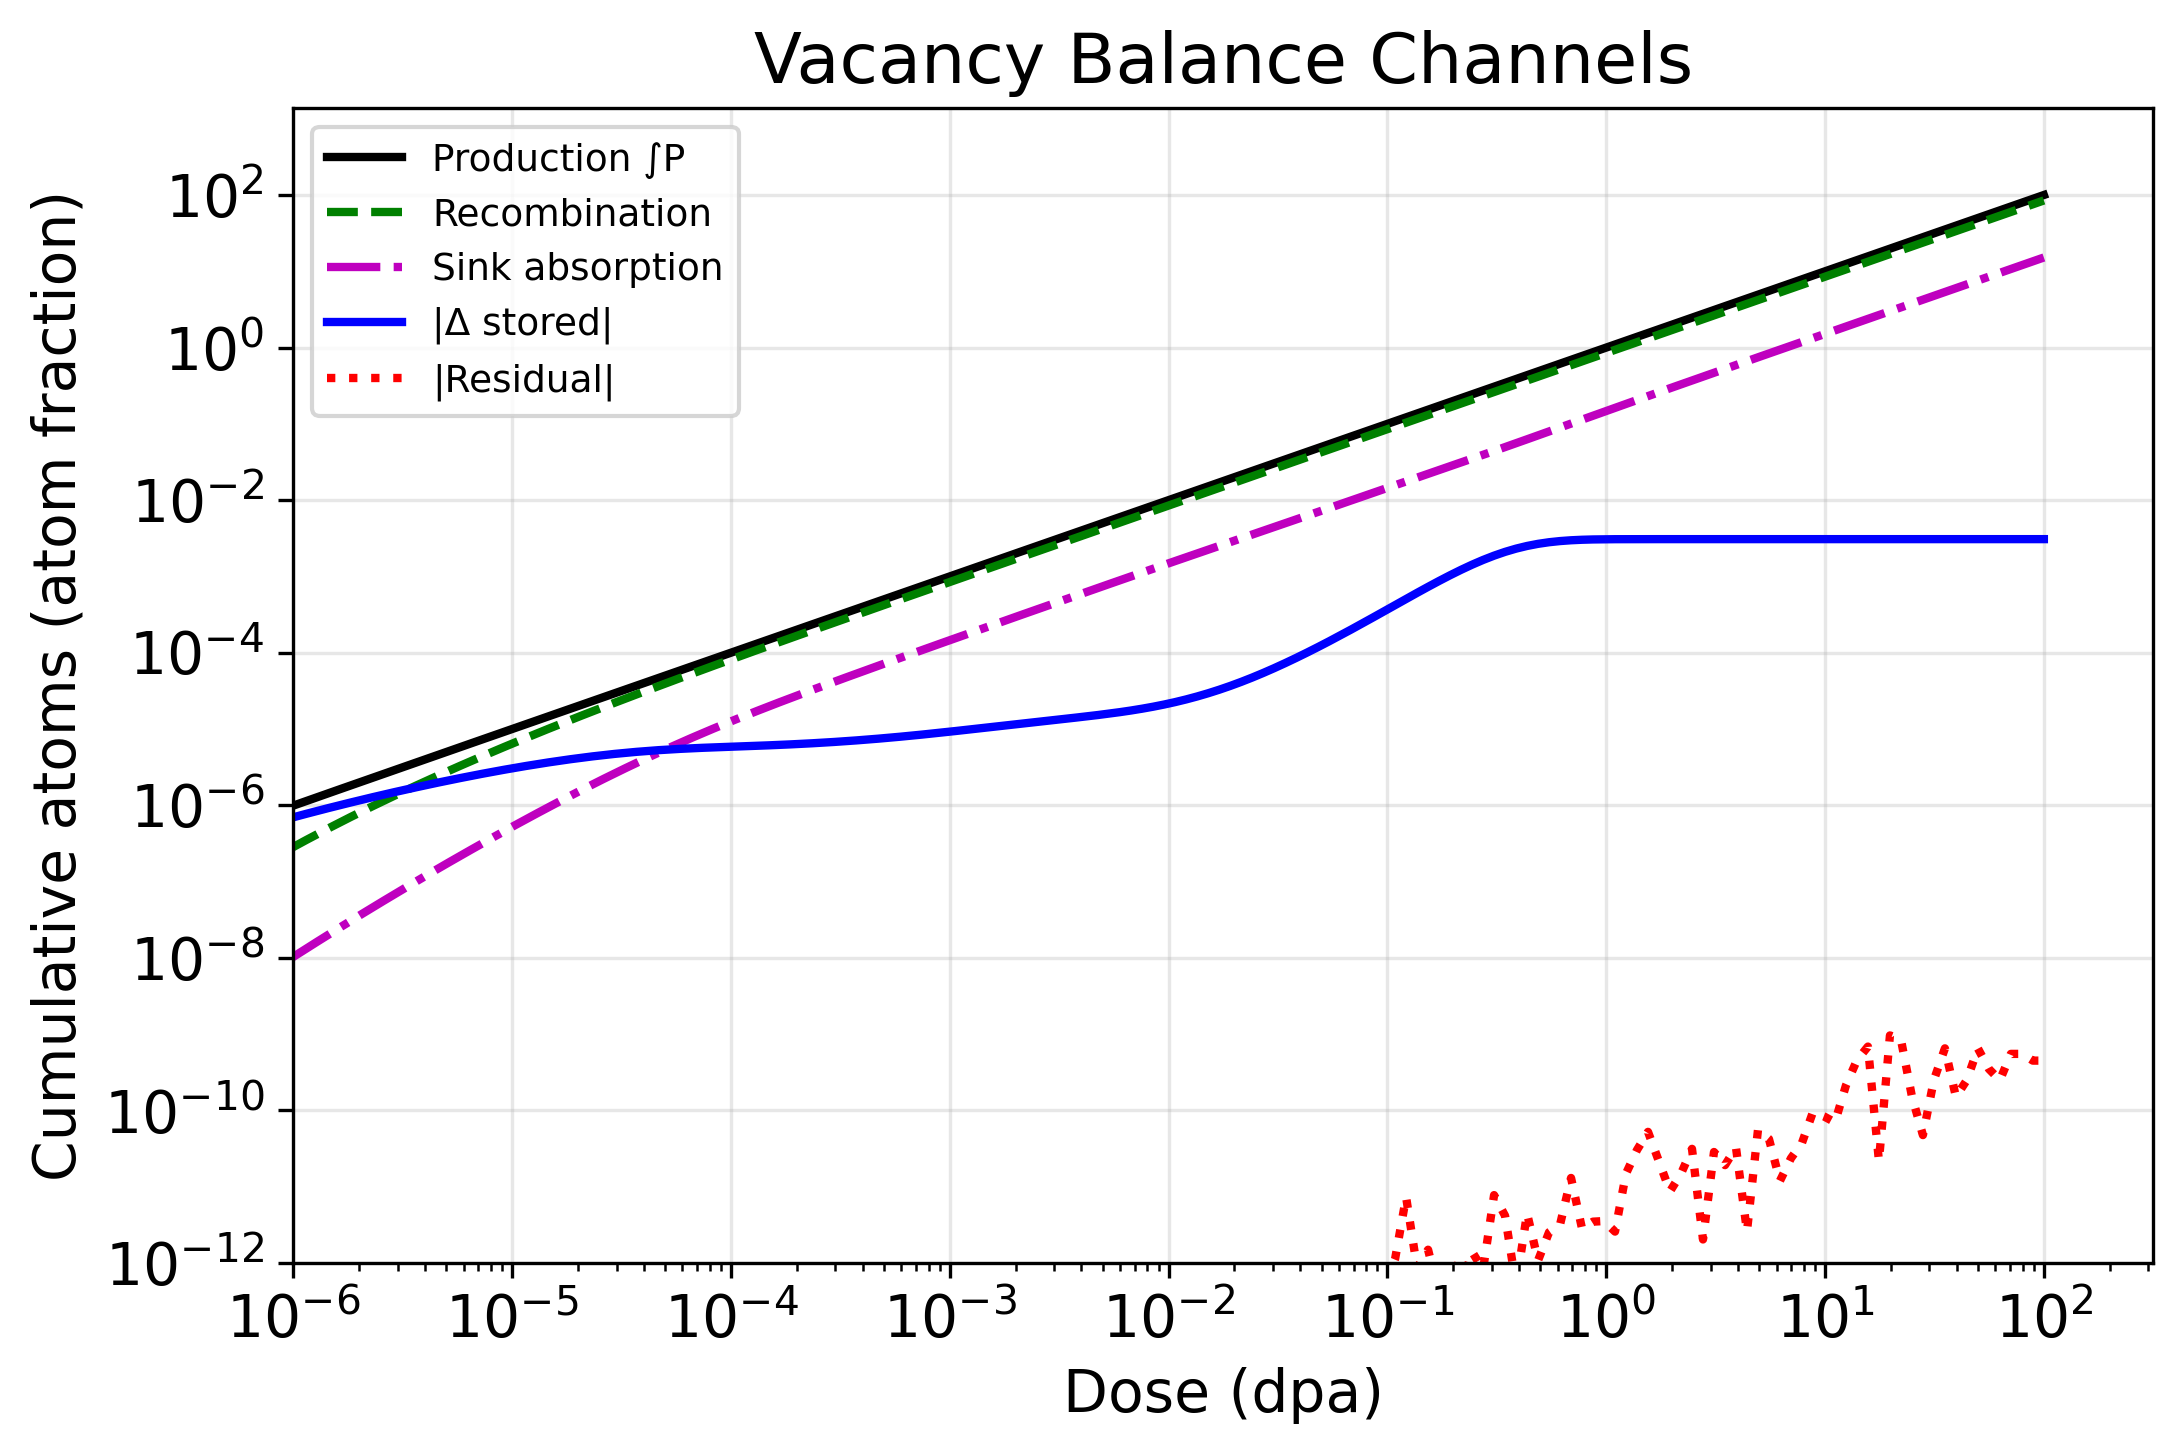
\includegraphics[width=0.49\linewidth]{figures/conservation_channels_v.png}
\caption{Interstitial (left) and vacancy (right) conservation channels. Production is balanced by recombination plus absorption at the sinks at every dose, confirming closure of the defect budget.}
\label{fig:conservation_channels_i}
\end{figure}

\begin{figure}[htbp]
\centering
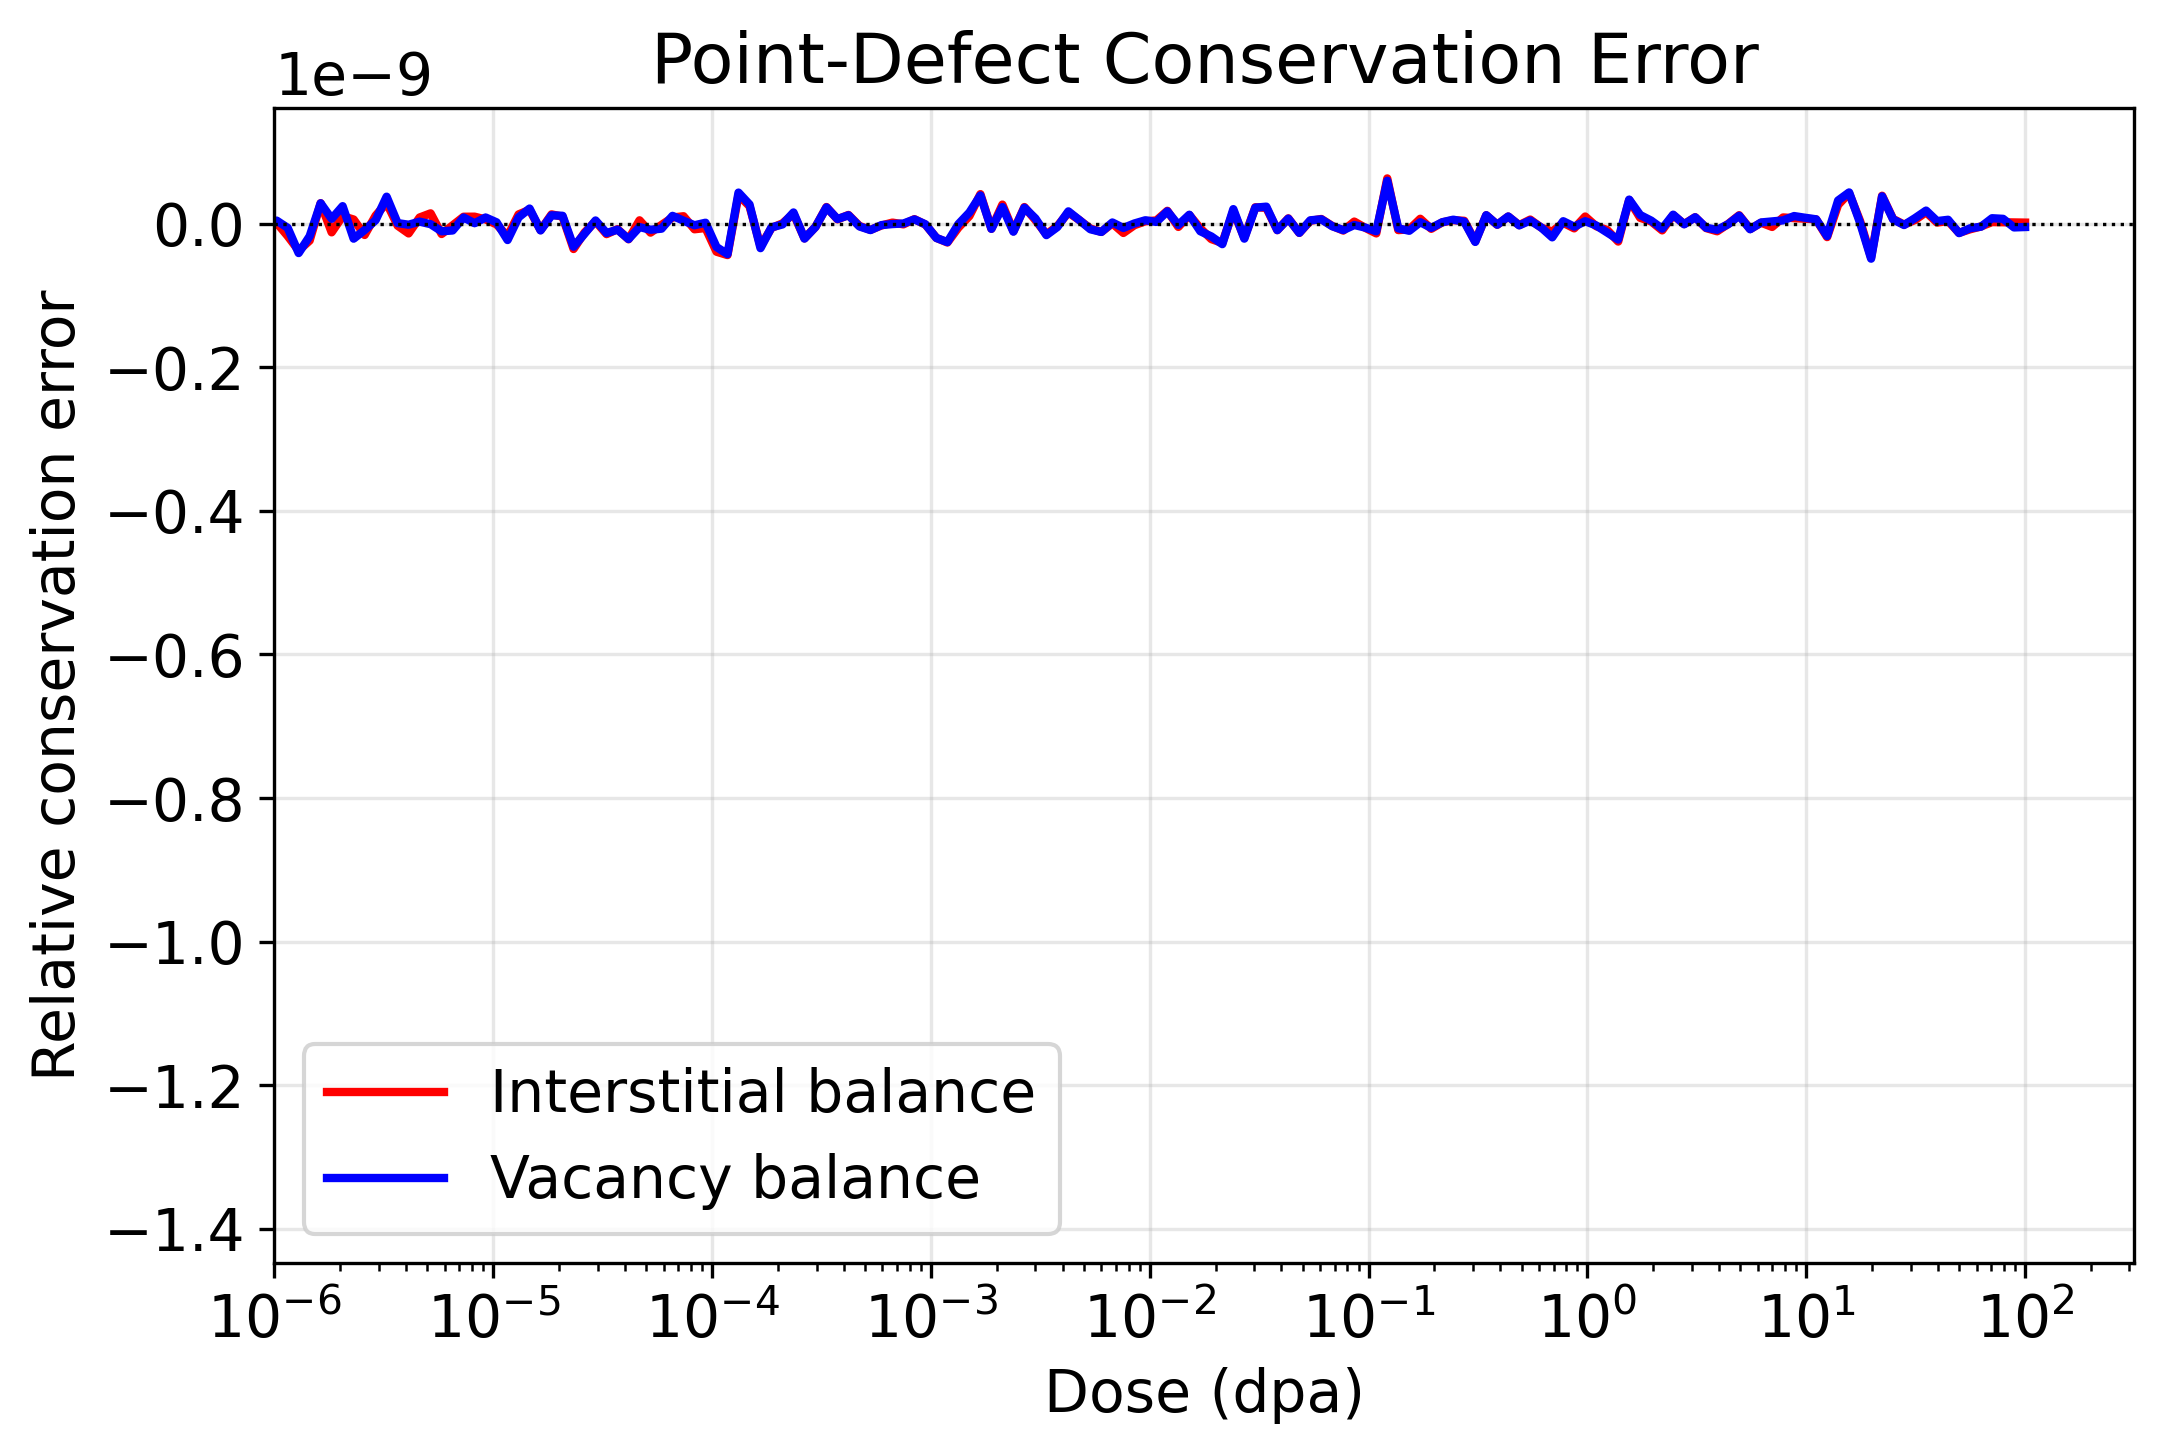
\includegraphics[width=0.7\linewidth]{figures/conservation_error.png}
\caption{Running relative error in the global defect balance, which remains at the round-off level over the full dose range, establishing that the reported transients and plateau are physical rather than numerical.}
\label{fig:conservation_error}
\end{figure}
%%%%%%%%%%%%%%


%==============================================================================
\section{The {\ZrM} Code Results}
\label{sec:results}

All results below are for a cubic domain of 1~$\mu$m side at
573~K and $G = 10^{-7}$~dpa/s, with zero applied stress, run to
30 dpa with output every 1 dpa. Every outer face carries the
Dirichlet condition, so the entire surface is grain boundary.

\subsubsection{Verification against {\ZrOd}}

Table~\ref{tab:verification} lists the ratio of interior 3-D values to the
corresponding {\ZrOd} values. Interior nodes are identified from the mobile
vacancy field, which saturates away from the absorbing boundary.

\begin{table}[htbp]
\centering
\caption{Ratio of \ZrM{} interior values to {\ZrOd}, as a function of dose.}
\label{tab:verification}
\begin{tabular}{@{}lcccccc@{}}
\toprule
dose [dpa] & $C_v$ & $C_i$ & $C_{2i}$ & $N_{\cloop}$ & $C_{\cloop}$ & $N_{\aloop}$ \\
\midrule
1  & 1.073 & 1.145 & 1.012 & 0.999 & 0.617 & 0.426 \\
5  & 0.988 & 1.124 & 0.446 & 0.999 & 0.647 & 0.547 \\
10 & 1.000 & 1.143 & 0.421 & 0.999 & 0.646 & 0.540 \\
20 & 1.008 & 1.155 & 0.413 & 0.999 & 0.643 & 0.534 \\
30 & 1.009 & 1.159 & 0.413 & 0.999 & 0.642 & 0.533 \\
\bottomrule
\end{tabular}
\end{table}

The mobile vacancy concentration and the \cloop{} loop density agree to better
than one percent at 30 dpa. More importantly, \emph{every ratio is
constant from about 5 dpa onwards}. As argued in Section~\ref{sec:intro},
this is the discriminating test: an error in a unit conversion or a rate constant
would be integrated by the loop populations and would appear as a drift. Its
absence indicates that the remaining differences are structural.

Two residuals are not yet explained. The \aloop{} loop density sits at
$0.53\times$ the 0-D value. The sign is consistent with the one nucleation
channel that remains unwired — the homogeneous clustering flux
$\Phi_{\rm clus} = R_{i,3i} + R_{2i,2i}$, which would add \aloop{} loops — but
the magnitude has not been demonstrated to follow from it. The di-interstitial
ratio falls from unity at 1 dpa to $0.41$ at saturation, indicating that
clusters are increasingly over-consumed as the loop sink population builds; this
points to the cluster weighting in the loop-absorption term rather than to their
production or dissociation, both of which are verified in
Table~\ref{tab:reactions}.

\subsubsection{Mobile defect fields}

Figure~\ref{fig:mobile} shows the four mobile species on a mid-plane cut at four
doses. The structure is the classical denuded zone: a plateau in the interior,
where production balances absorption at the network and at the loops, falling to
the thermal equilibrium concentration at the boundary over a depletion length
\begin{equation}
\ell = \frac{1}{\sqrt{k^2}} \approx 73~\text{nm}
\qquad\text{for}\qquad k^2 \simeq \rho_N = 1.88\times10^{14}~\text{m}^{-2},
\label{eq:depletion}
\end{equation}
which is small compared with the 1~$\mu$m domain. The interior is
therefore approximately fourteen depletion lengths across, which is what makes
the comparison with the well-mixed 0-D model meaningful.

\begin{figure}[htbp]
\centering
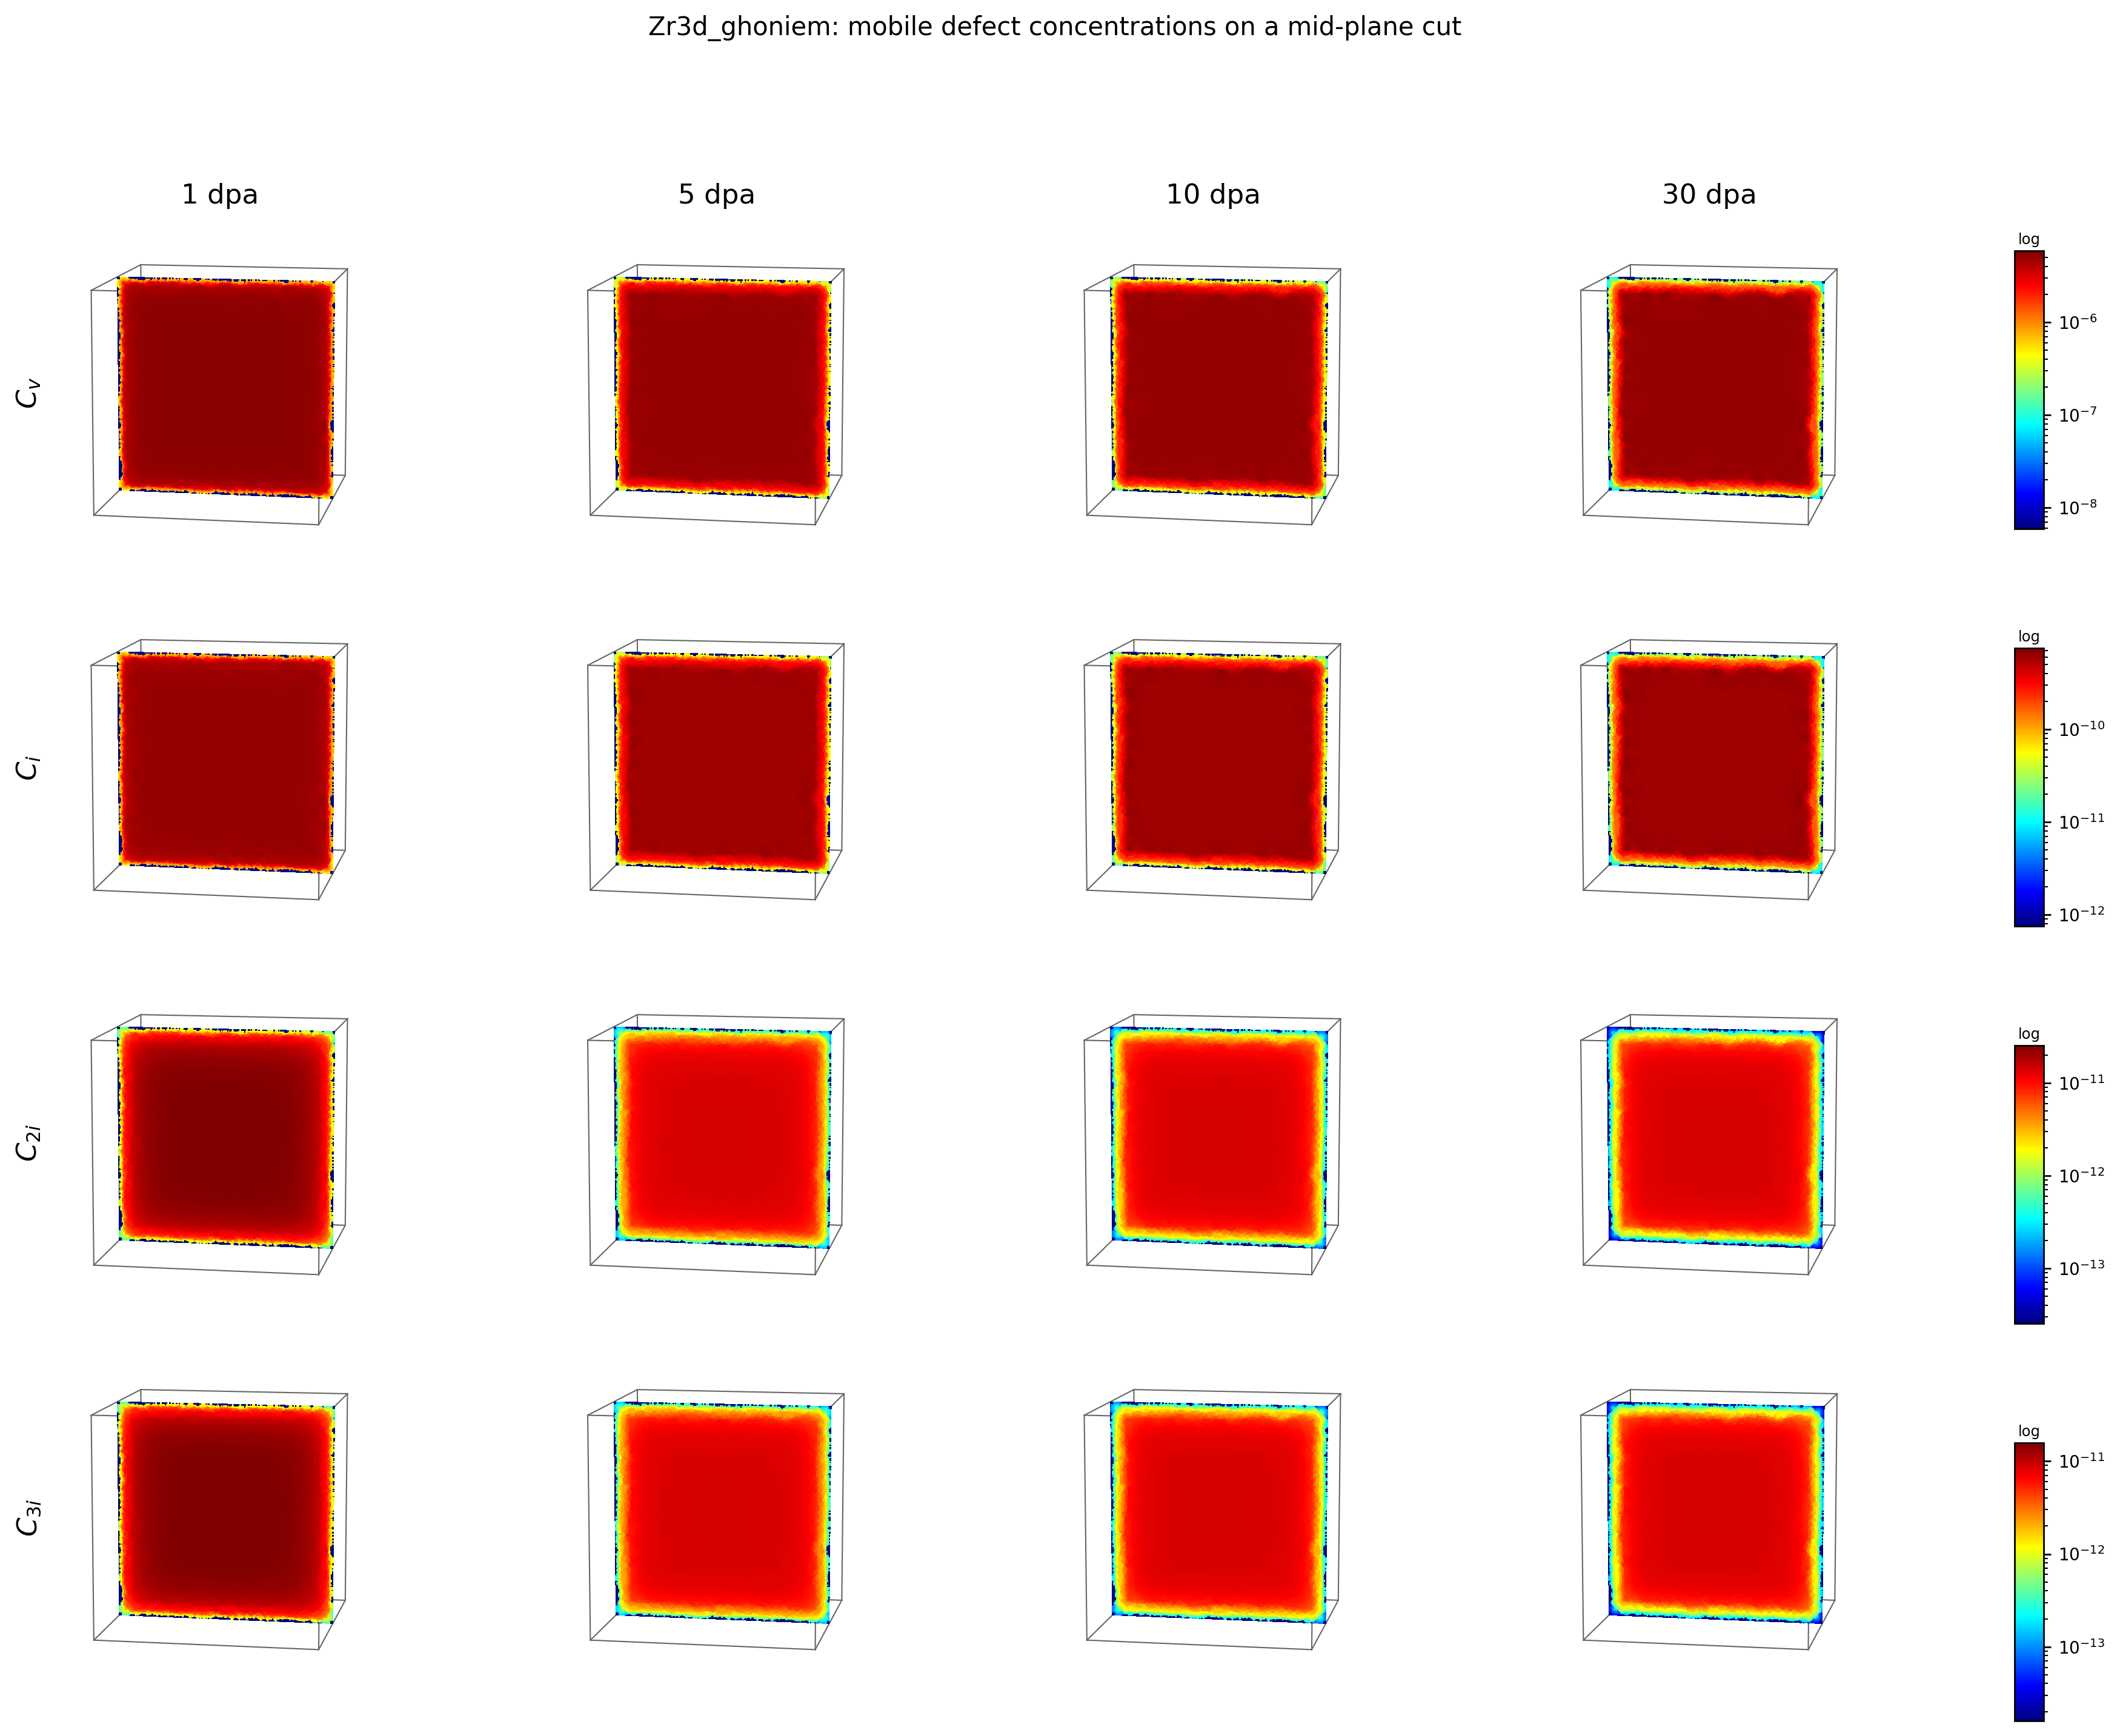
\includegraphics[width=\textwidth]{figures/mobile_fields.png}
\caption{Mobile defect concentrations $C_v$, $C_i$, $C_{2i}$ and $C_{3i}$ on an
interior mid-plane cut, at 1, 5, 10 and 30 dpa. The color scale is
logarithmic over three decades below the maximum, which places the color range
across the depletion shell rather than on the interior plateau. The depleted
layer thickens with dose as the loop sink strength grows.}
\label{fig:mobile}
\end{figure}

The depleted layer visibly thickens with the dose. This is not a change in the
diffusivity but in the sink strength: as loops accumulate, $k^2$ rises, the
interior concentration falls, and the balance between boundary absorption and
bulk absorption shifts.

\subsubsection{Loop density and content fields}

Figures~\ref{fig:idens} and~\ref{fig:icont} show the four immobile families.
Their spatial structure is the \emph{inverse} of the mobile fields, and the
reason is instructive. Cascade nucleation is spatially uniform, being
proportional only to the dose rate. Loop removal, however, occurs by coalescence,
whose rate is set by the absorbed mobile flux. Near the boundary that flux
vanishes, so loops are created at the full rate and never removed: the density
rises steeply while the size of each loop falls.

The two loop types then behave in \emph{opposite} senses, and the distinction
matters for the growth strain. For the \aloop{} families the density rises by
more than three orders of magnitude toward the boundary while the mean number of
defects per loop falls only by a factor of about six, so the density excess
dominates and the stored content is \emph{enhanced} at the boundary. For the
\cloop{} family the density is set by the balance between cascade nucleation and
embryo dissolution, Eq.~\eqref{eq:dNdt}, which involves no mobile flux at all and
is therefore almost uniform in space; the size deficit is then unopposed and the
stored content is \emph{depleted} at the boundary. Both behaviors are visible in
Fig.~\ref{fig:gbcont}.

\begin{figure}[htbp]
\centering
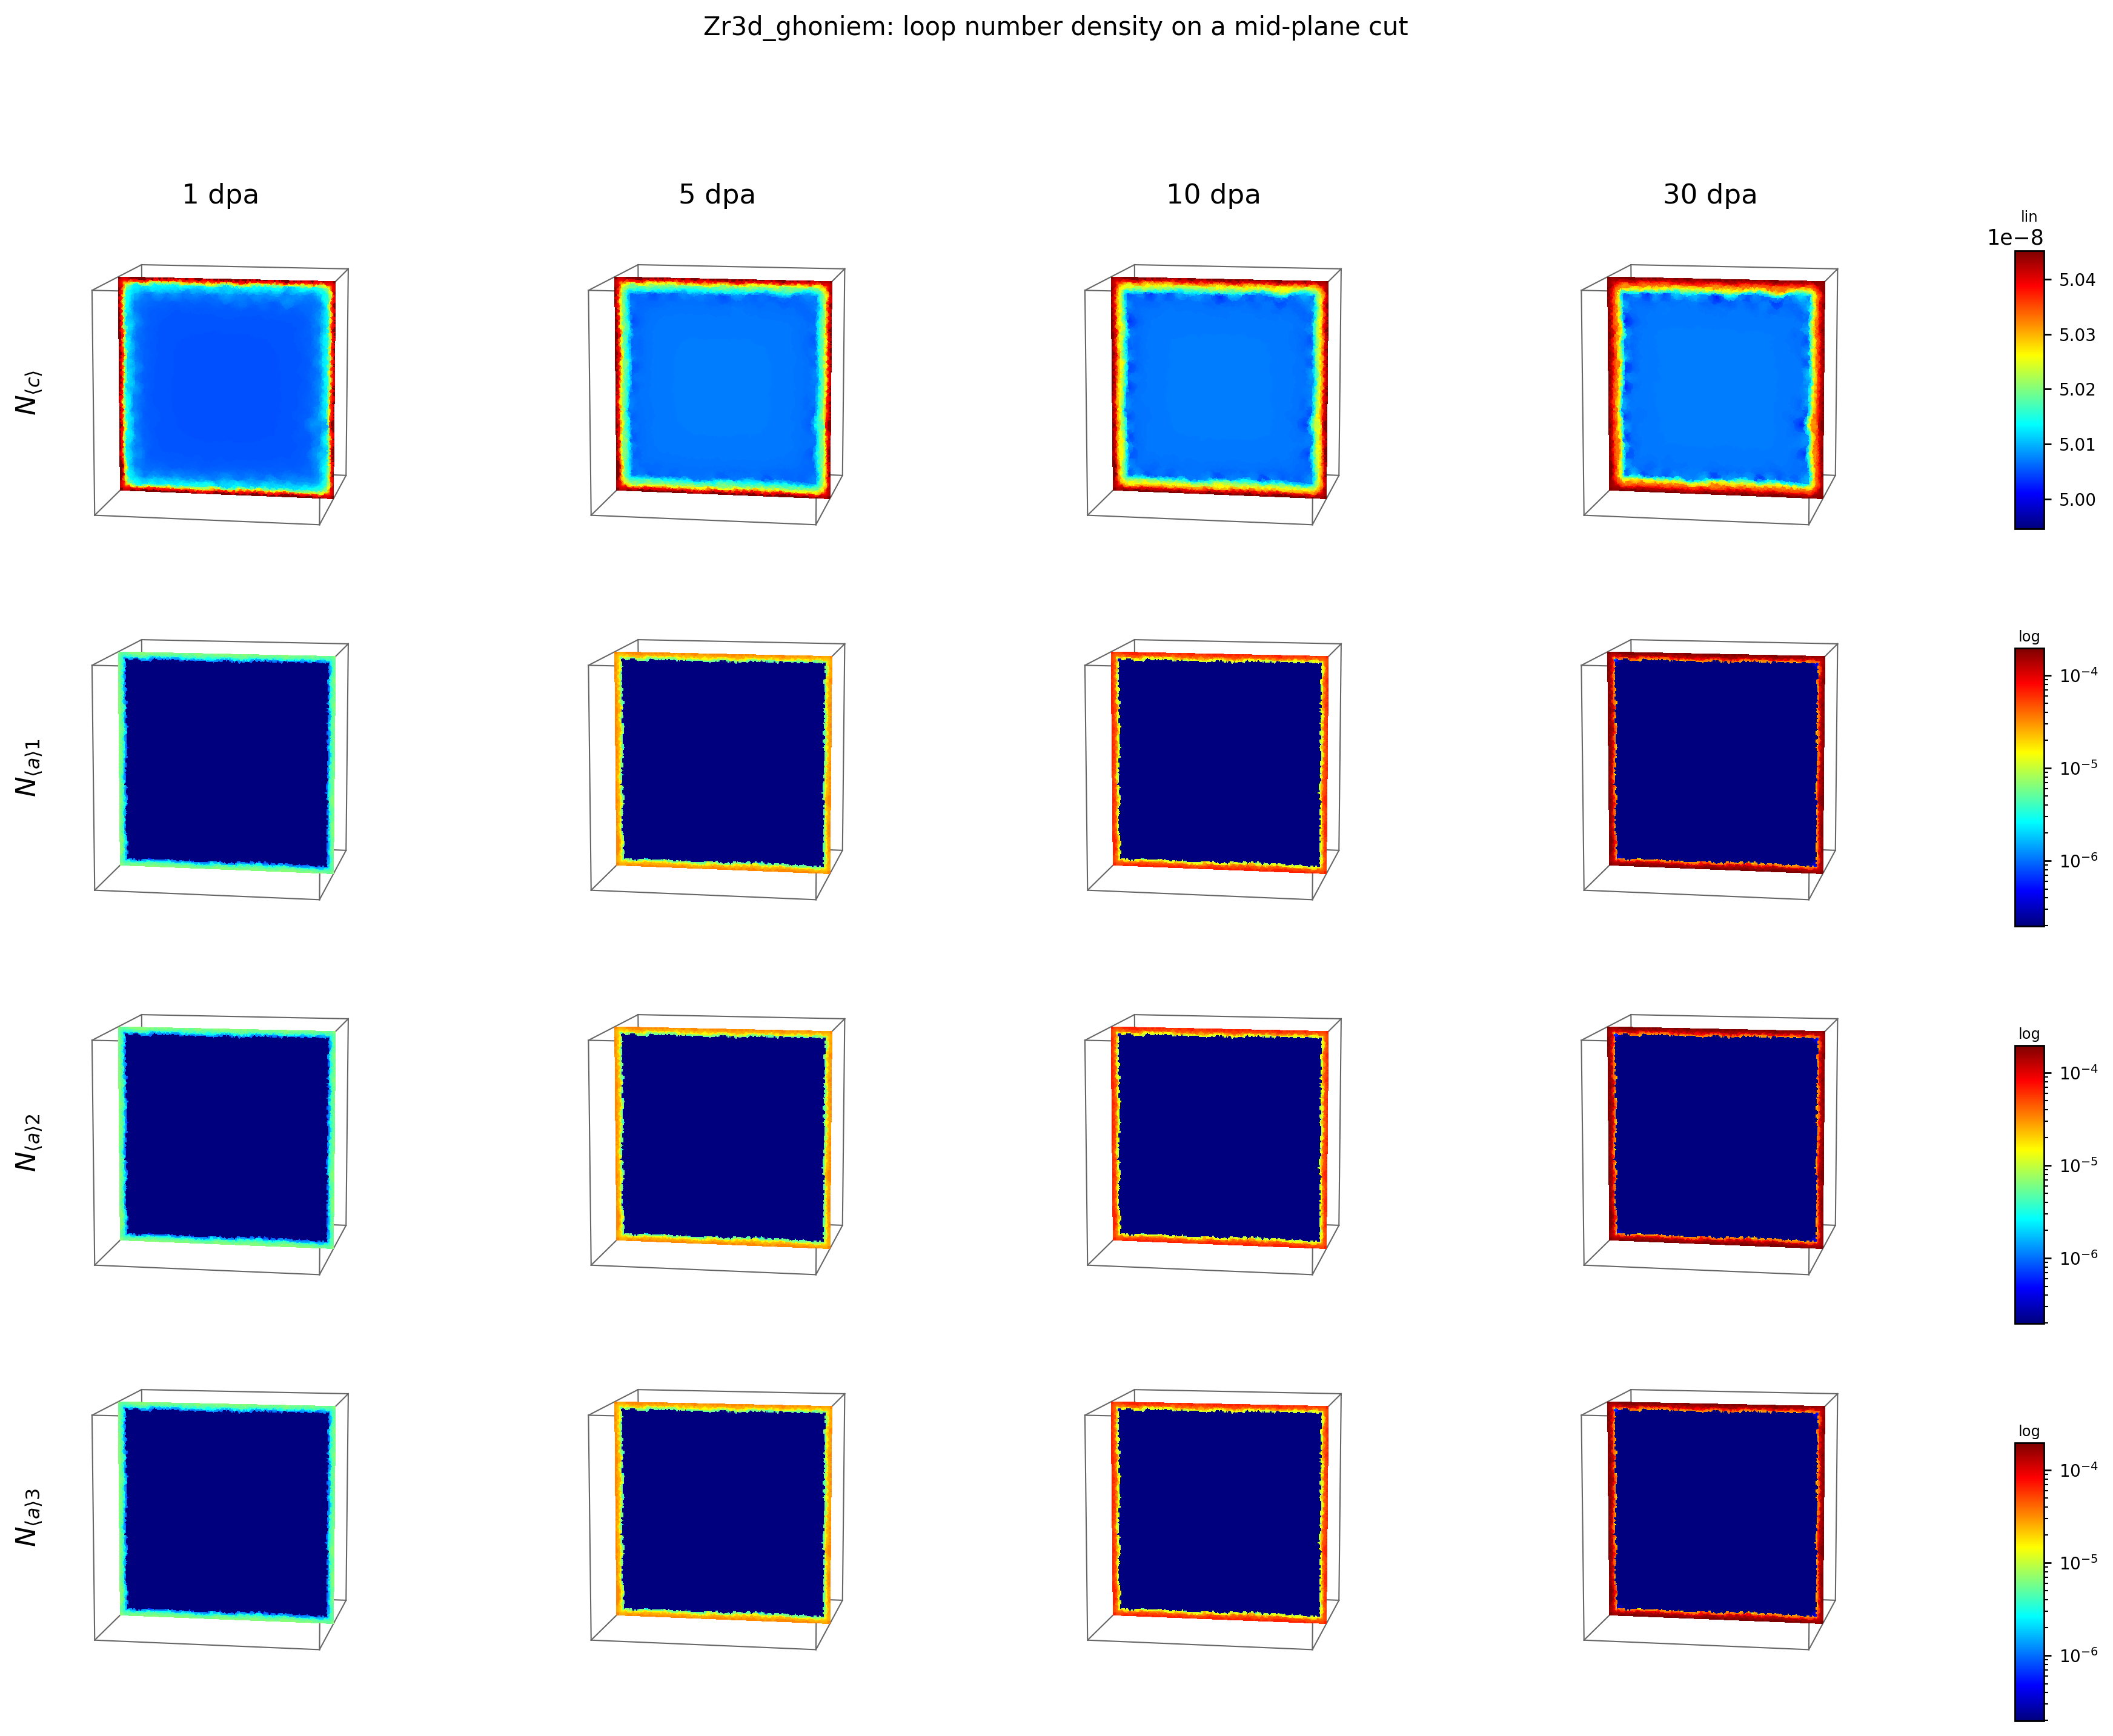
\includegraphics[width=\textwidth]{figures/immobile_density_fields.png}
\caption{Loop number density for the basal \cloop{} family and the three
prismatic \aloop{} families. At zero applied stress the three \aloop{} panels
must be identical, and are; this is a check on the crystallography. Note the
accumulation adjacent to the grain boundary.}
\label{fig:idens}
\end{figure}

\begin{figure}[htbp]
\centering
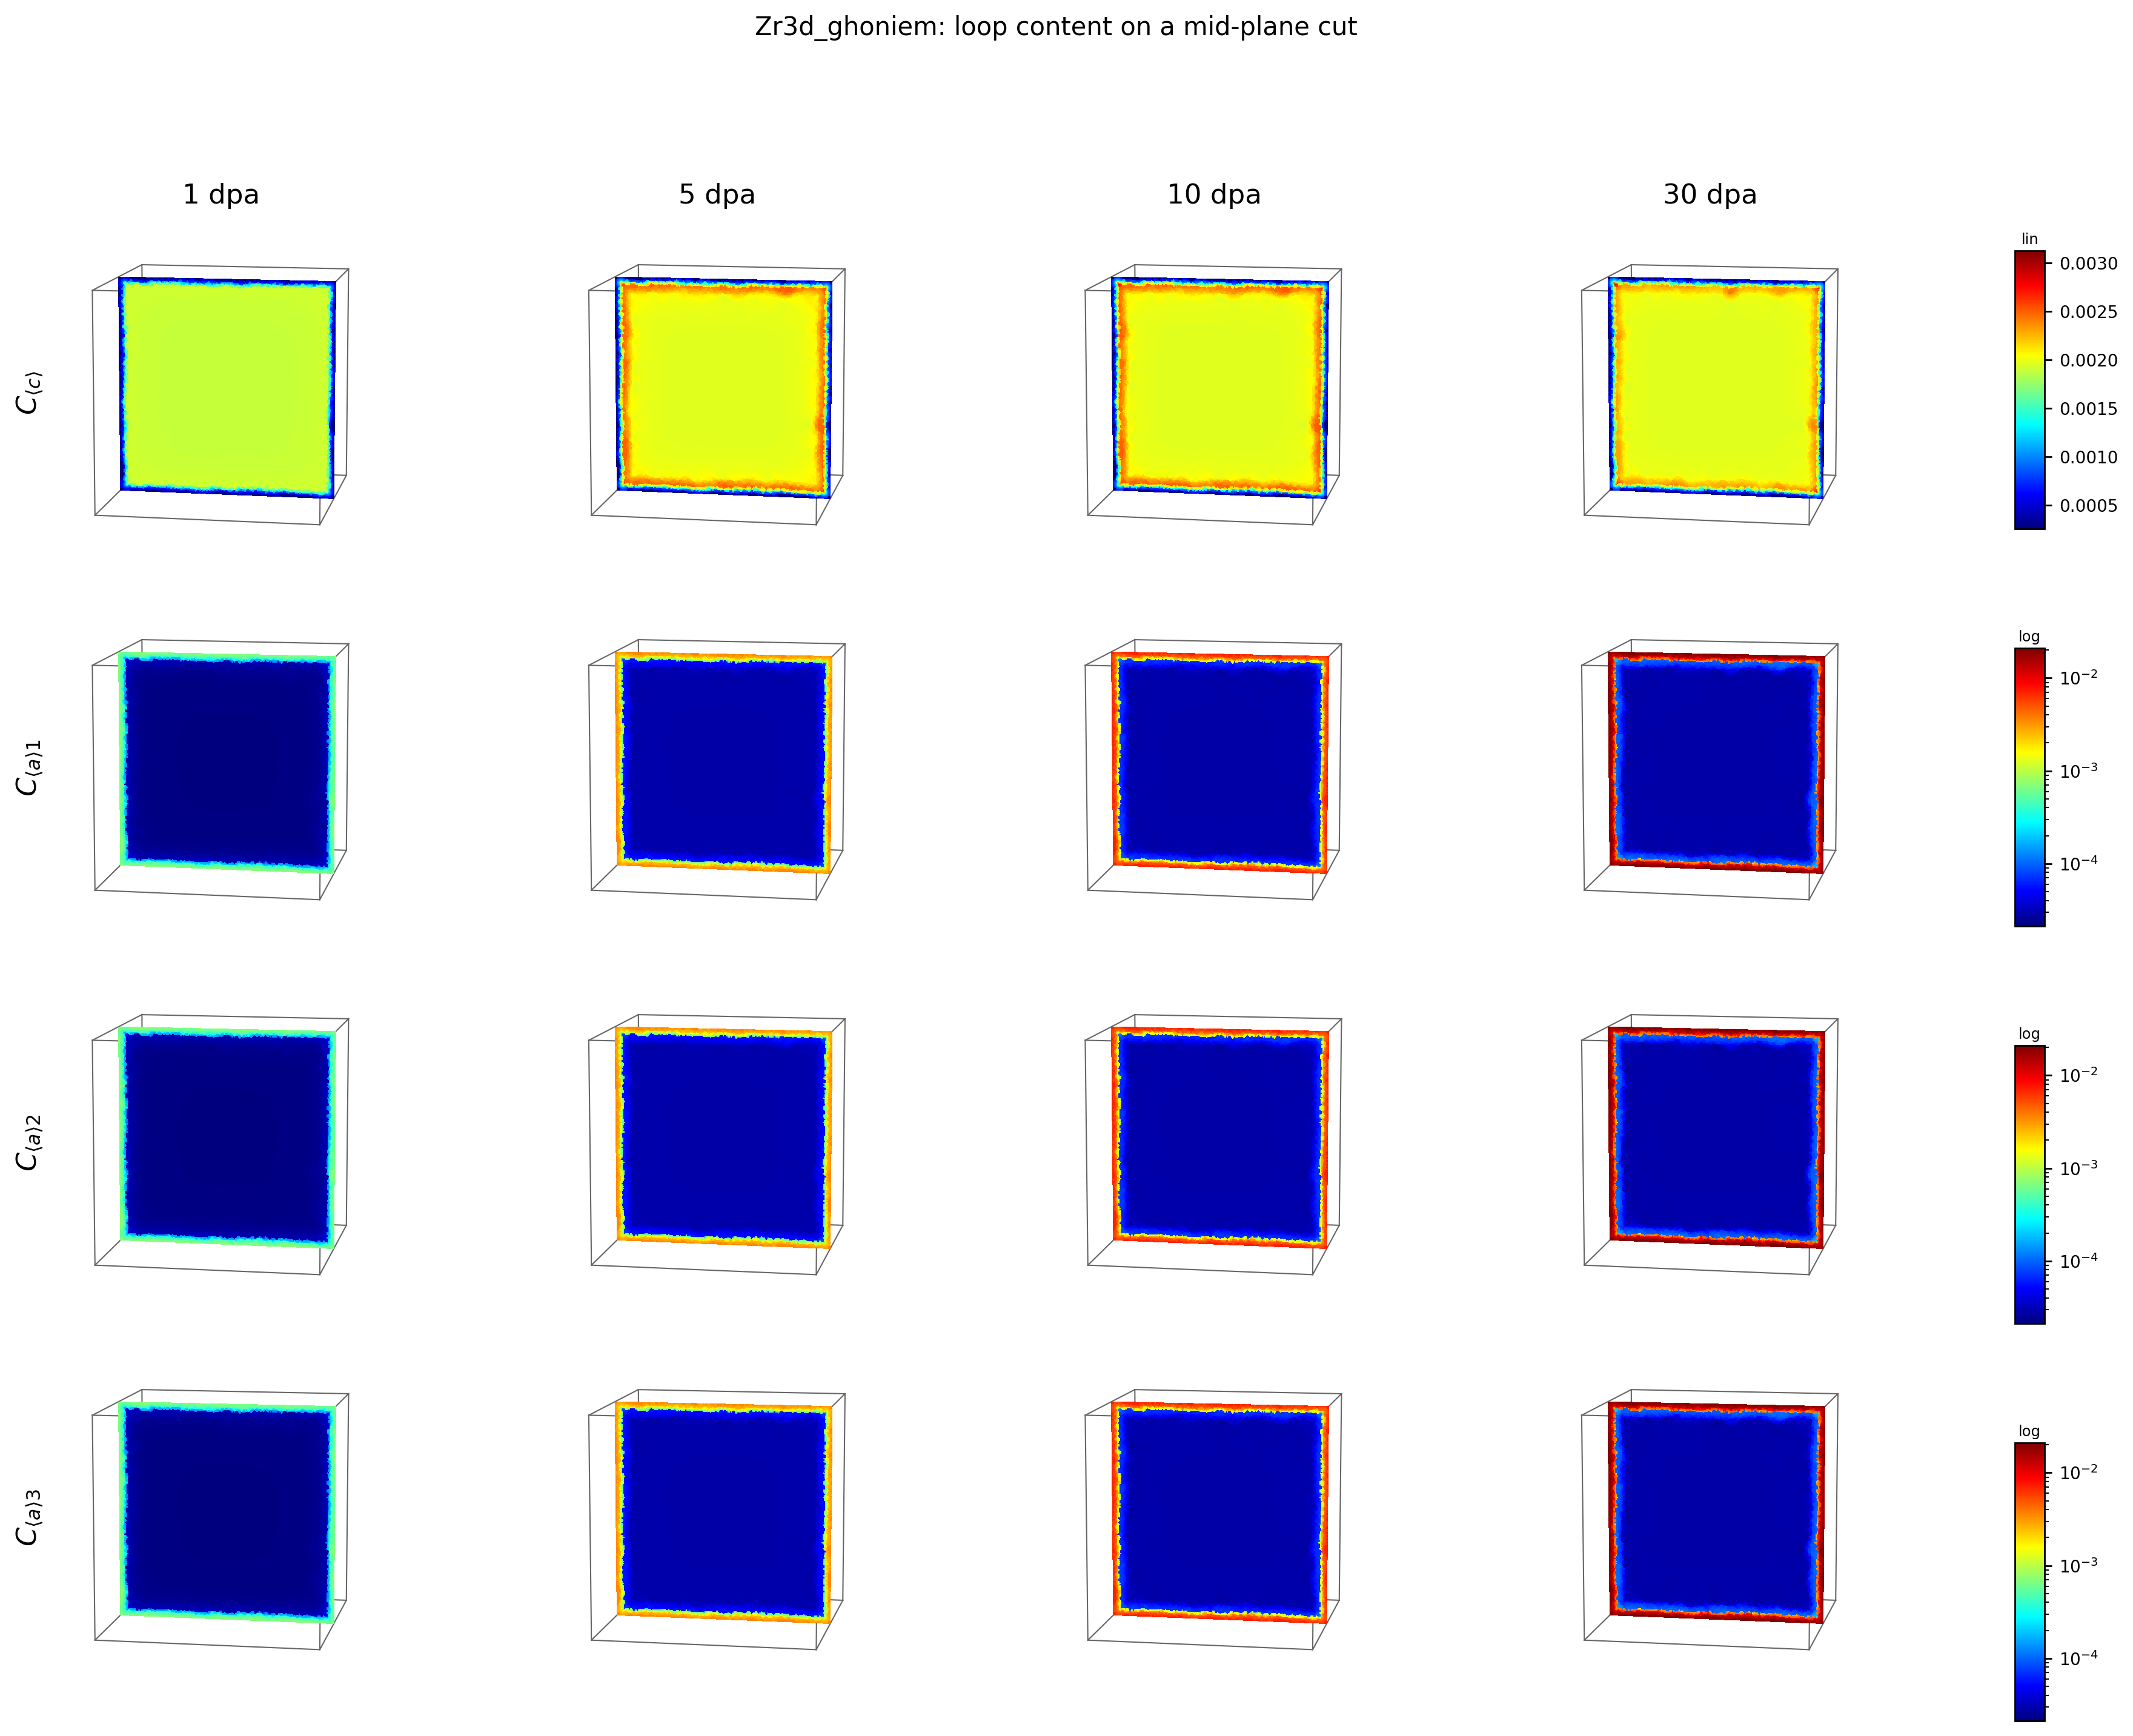
\includegraphics[width=\textwidth]{figures/immobile_content_fields.png}
\caption{Stored defect content of the four loop families. The \aloop{} families
are \emph{enhanced} at the boundary, where the density excess outweighs the size
deficit; the \cloop{} family is \emph{depleted} there, its density being almost
uniform in space so that the size deficit is unopposed.}
\label{fig:icont}
\end{figure}

The three prismatic panels in Fig.~\ref{fig:idens} are identical, as they must be
at zero applied stress. This is the internal consistency check identified in
Section~\ref{sec:structure}, and it is a sensitive one: an error in the Burgers
vector components produced clearly unequal densities and was detected this way.

\subsubsection{Loop populations}

Figure~\ref{fig:loopsc} shows the \cloop{} population overlaid on its own content
field, with each platelet drawn at the local mean radius and in its correct habit
plane. Figure~\ref{fig:loopsa} shows one prismatic family. The platelet radii are
exaggerated by a factor of 45: the true mean radius is of the order of 4~nm
against a 1~$\mu$m box, so an honest scale would draw nothing. The
relative sizes remain meaningful.

\begin{figure}[htbp]
\centering
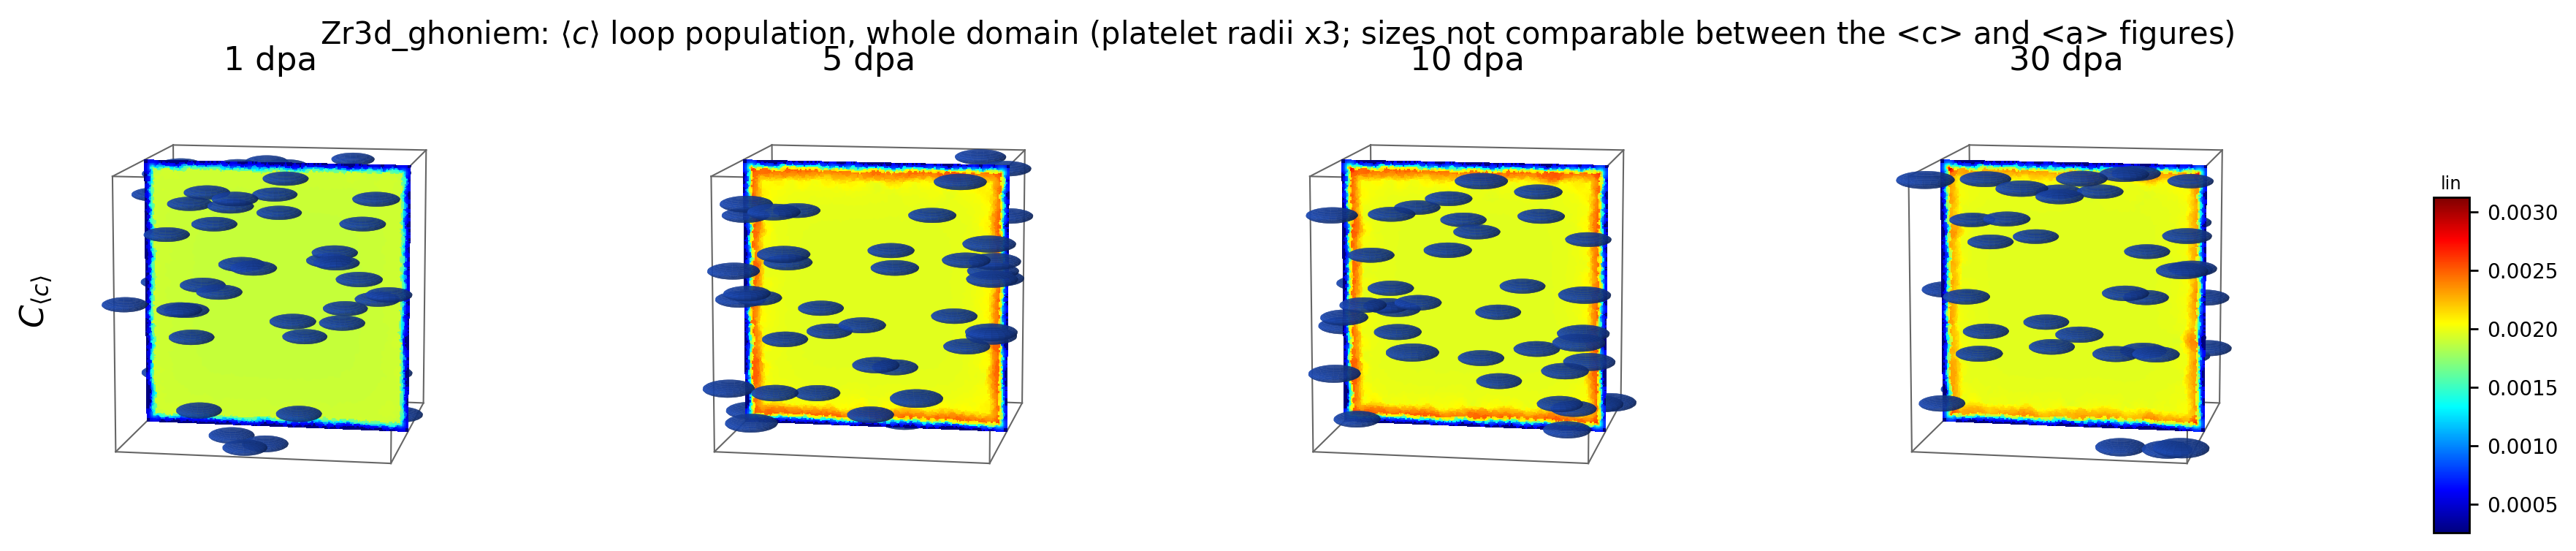
\includegraphics[width=\textwidth]{figures/loops_c_overlay.png}
\caption{Basal \cloop{} vacancy loop population. Platelets lie in the basal
plane, consistent with the $\langle c\rangle$ Burgers vector.}
\label{fig:loopsc}
\end{figure}

\begin{figure}[htbp]
\centering
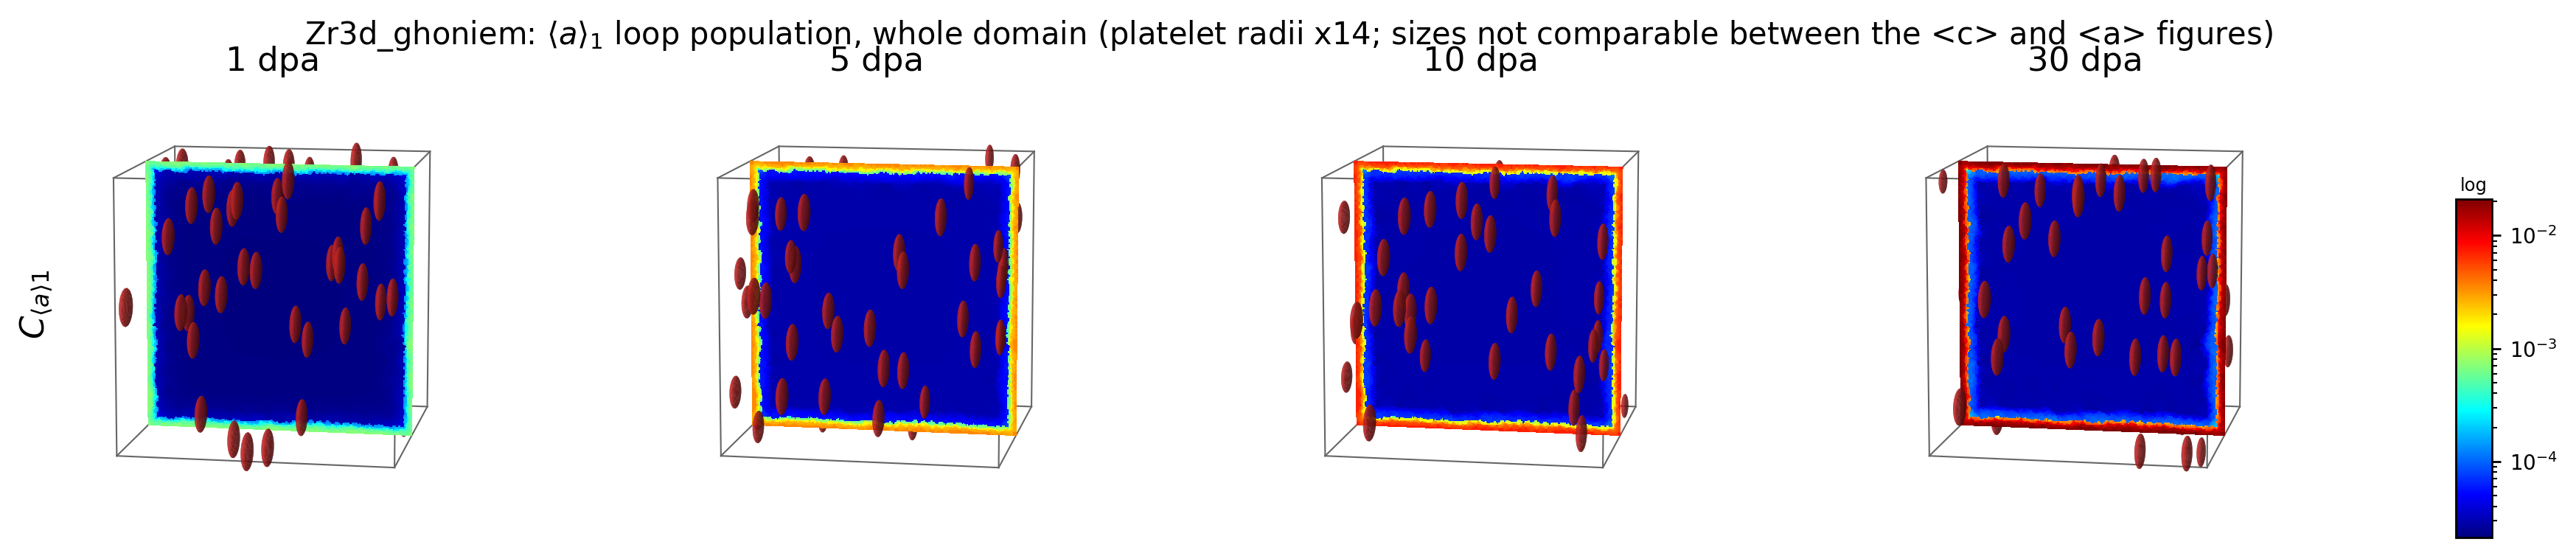
\includegraphics[width=\textwidth]{figures/loops_a1_overlay.png}
\caption{One of the three prismatic \aloop{} interstitial loop families. The
habit plane differs from Fig.~\ref{fig:loopsc}, as it must.}
\label{fig:loopsa}
\end{figure}

The \cloop{} population is of particular interest because it controls the
$c$-axis component of irradiation growth. Its number density saturates almost
immediately, at the balance $N^\ast = \dot{N}_{\rm nuc}\tau_{vL}$ between cascade
nucleation and embryo dissolution, and thereafter the population evolves only
through the size of the surviving loops.

\subsubsection{Grain-boundary profiles}

Figures~\ref{fig:gbmob} to~\ref{fig:gbsize} present radially averaged profiles
against distance from the grain boundary. Because every face carries the Dirichlet
condition, the distance is the minimum over all six faces, and each bin averages
over the faces and over position within a face.

\begin{figure}[htbp]
\centering
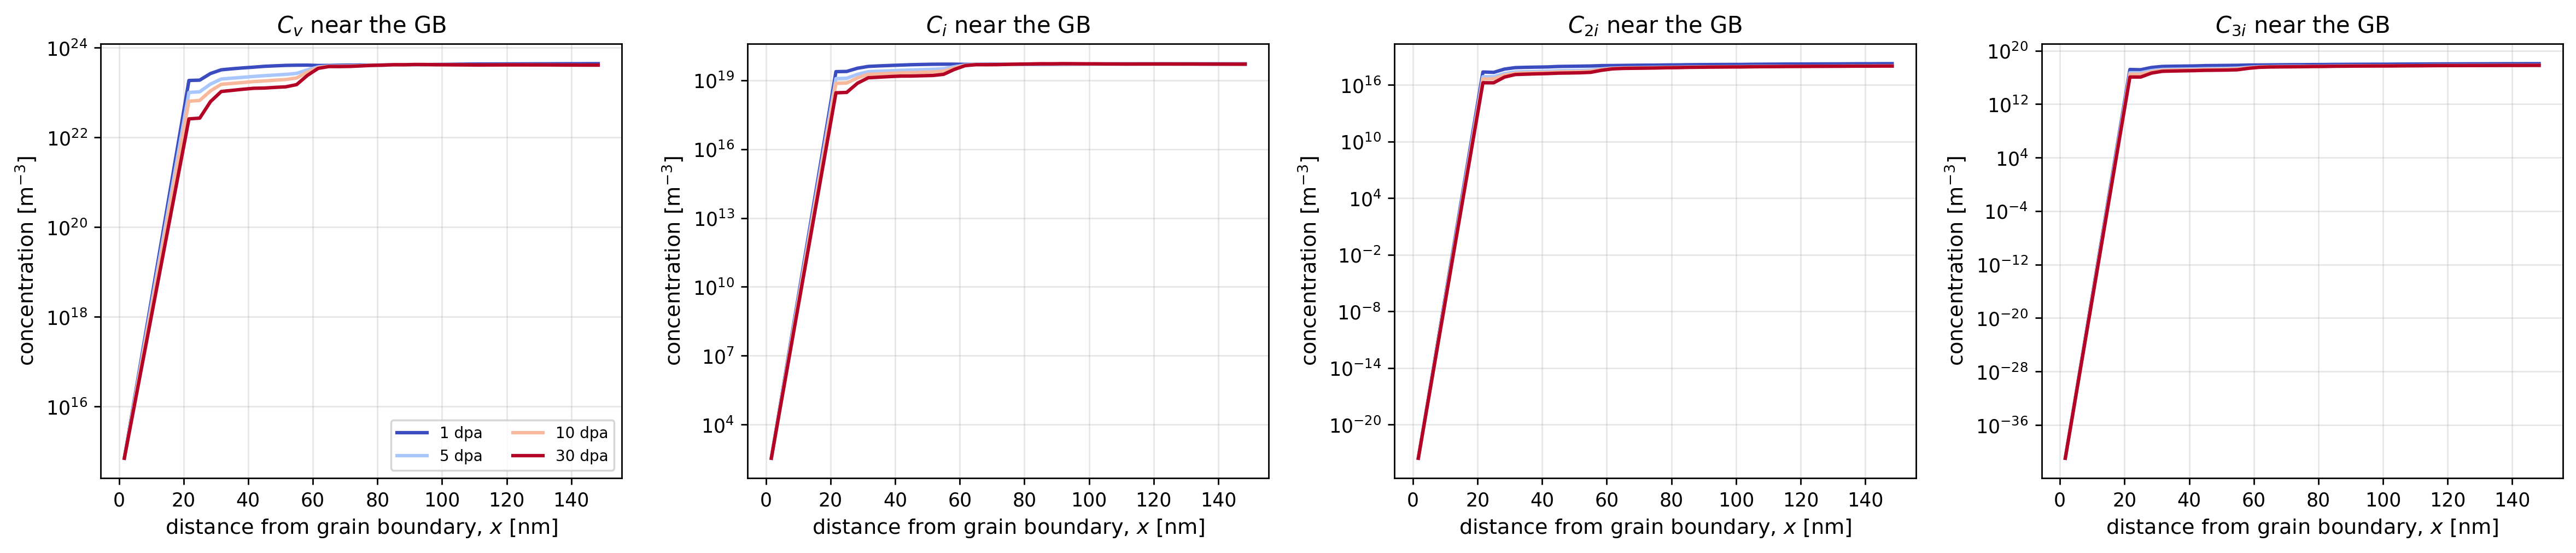
\includegraphics[width=\textwidth]{figures/gb_mobile_profiles.png}
\caption{Mobile defect concentrations against distance from the grain boundary.
The recovery length is the depletion length $\ell \approx 73~nm$; beyond
roughly 300~nm the profiles are flat, confirming that the interior is well
mixed.}
\label{fig:gbmob}
\end{figure}

\begin{figure}[htbp]
\centering
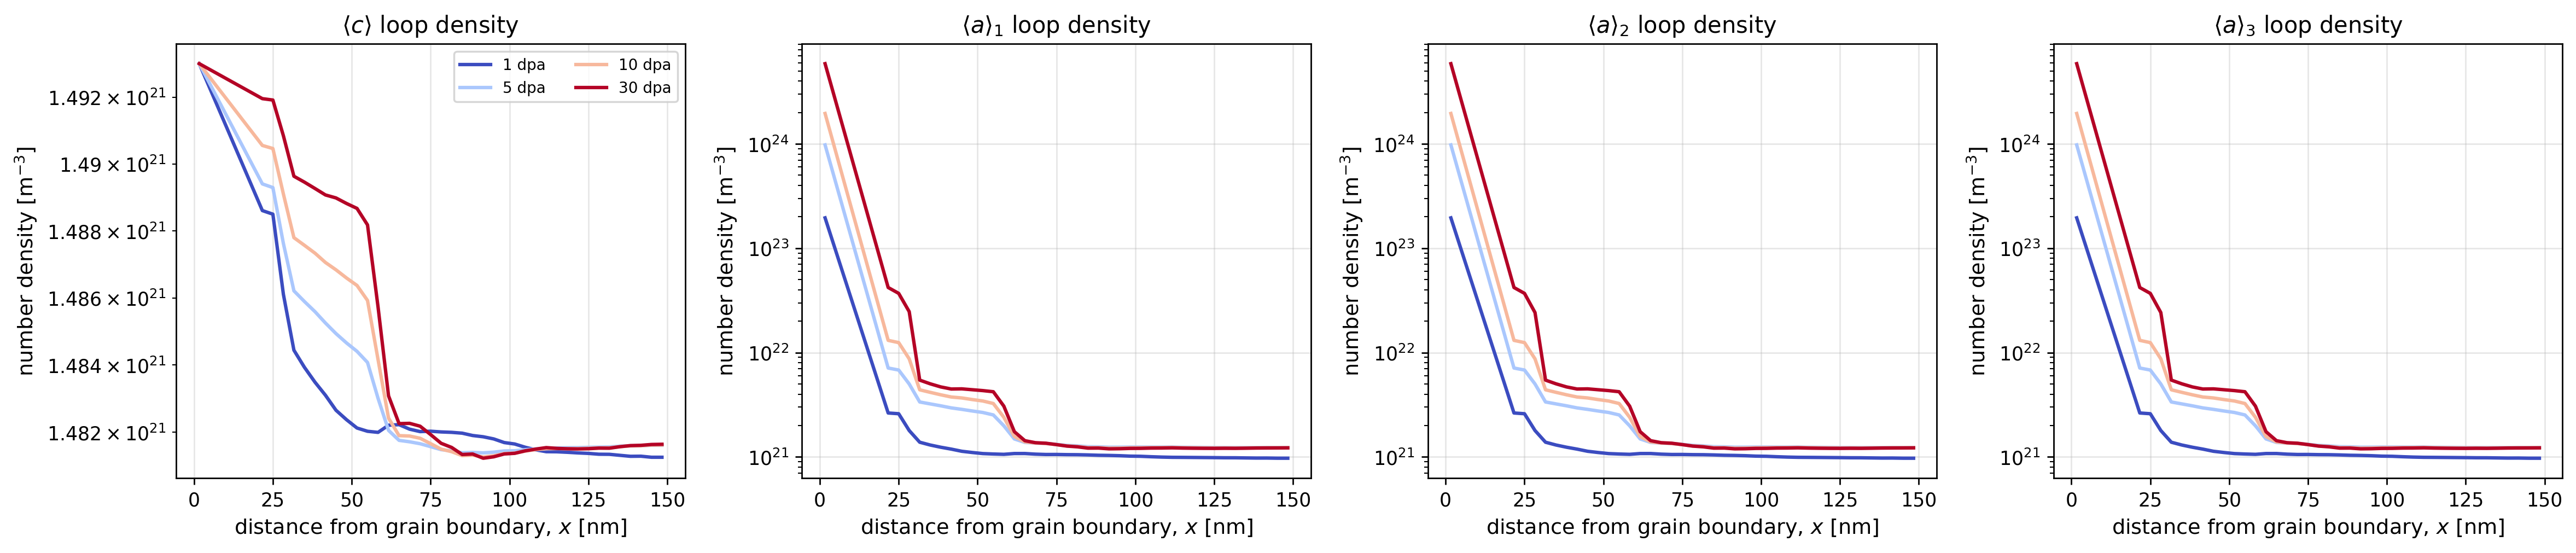
\includegraphics[width=\textwidth]{figures/gb_density_profiles.png}
\caption{Loop number density against distance from the grain boundary. The
\aloop{} families rise by more than three orders of magnitude within the first
few tens of nanometres.}
\label{fig:gbdens}
\end{figure}

\begin{figure}[htbp]
\centering
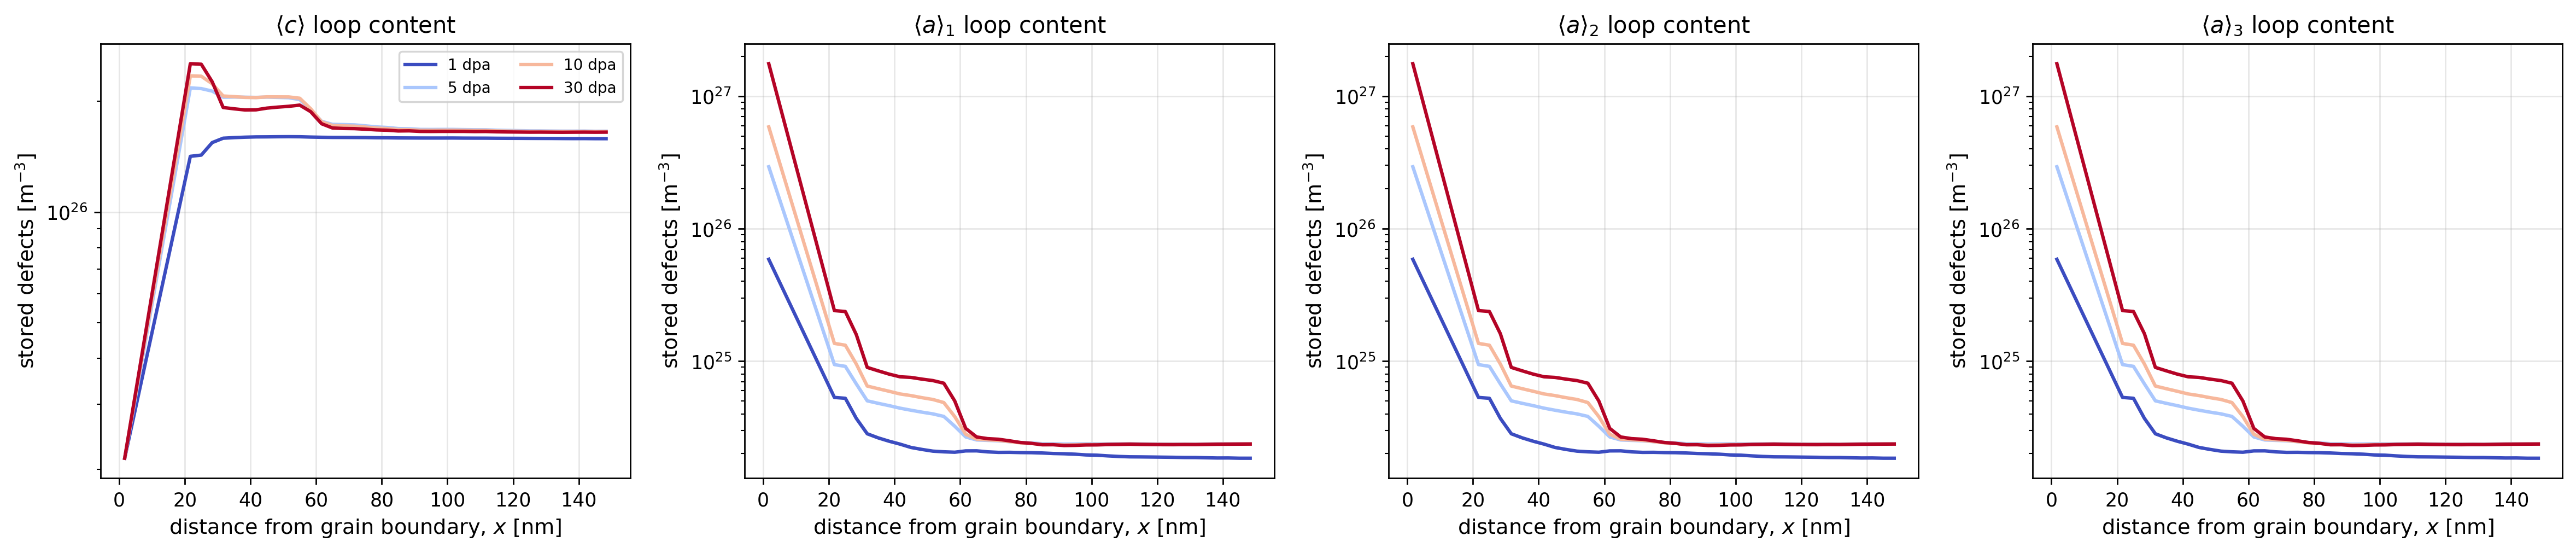
\includegraphics[width=\textwidth]{figures/gb_content_profiles.png}
\caption{Stored defect content against distance from the grain boundary.}
\label{fig:gbcont}
\end{figure}

\begin{figure}[htbp]
\centering
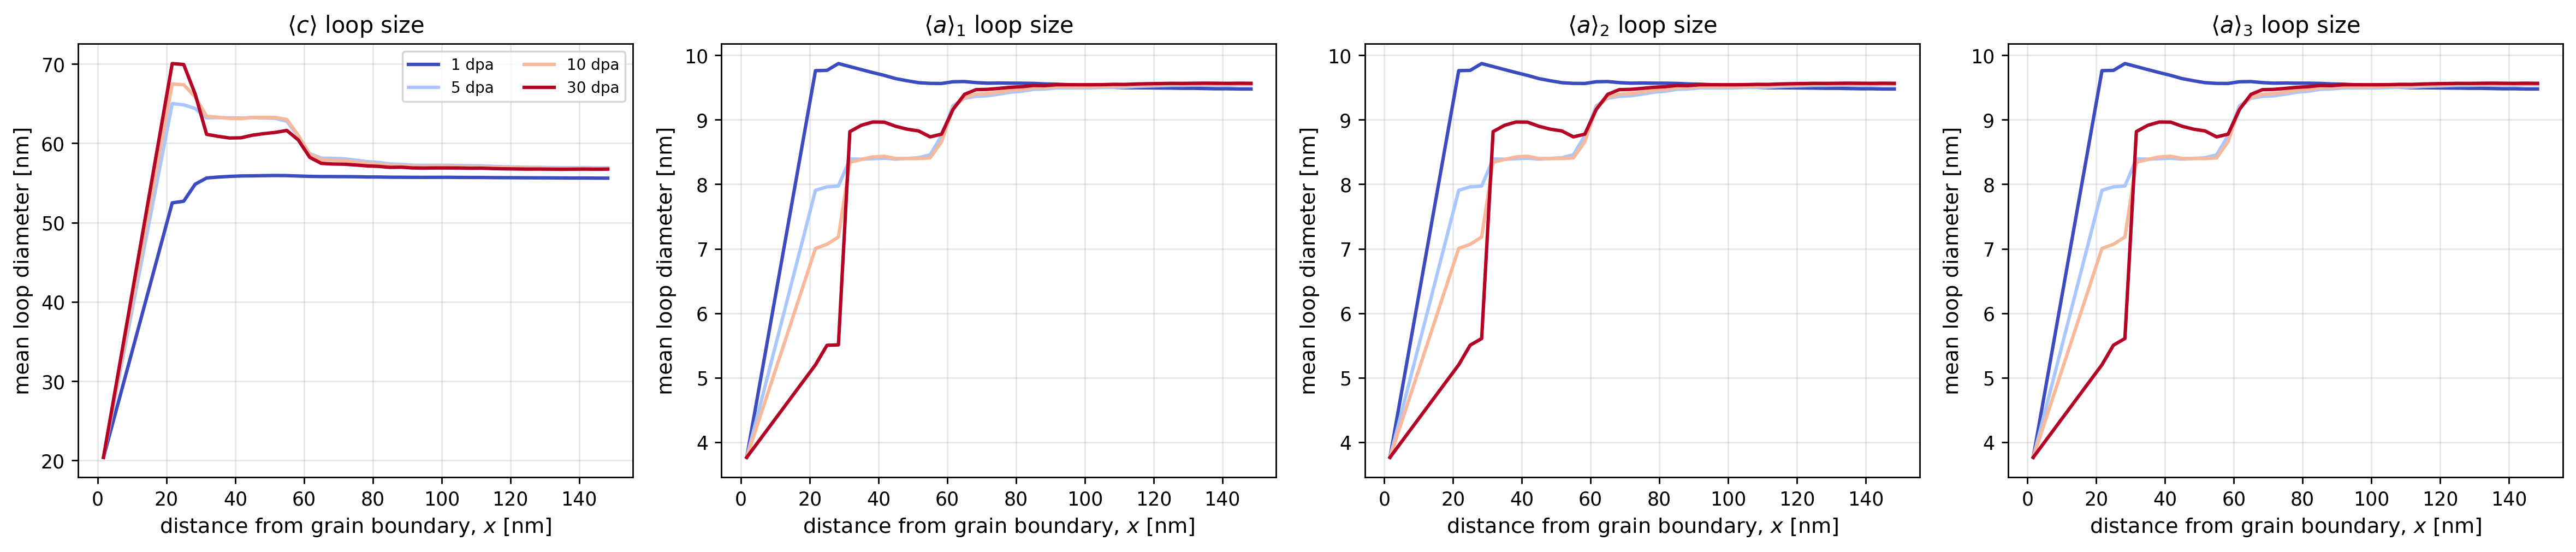
\includegraphics[width=\textwidth]{figures/gb_size_profiles.png}
\caption{Mean loop diameter against distance from the grain boundary. The
diameter is formed from the binned mean content and density, not by averaging
nodal diameters: size is a ratio of two fields, and the mean of a ratio is not
the ratio of the means.}
\label{fig:gbsize}
\end{figure}

Figures~\ref{fig:gbdens} and~\ref{fig:gbsize} together give the physical picture
of the denuded zone: adjacent to the boundary, there are \emph{many small} loops,
and in the interior, \emph{fewer large} ones. The total stored content, which is
what enters the growth strain, is nevertheless depleted at the boundary
(Fig.~\ref{fig:gbcont}), since the size deficit outweighs the density excess.

\subparagraph{A caution.} The \aloop{} density adjacent to the boundary grows
without bound, linearly with dose. The mechanism is the one described above:
uniform cascade nucleation with a removal channel that requires a mobile flux that the
boundary condition suppresses. Physically, a grain boundary is also a sink for
loops that grow into it, and that channel is absent from the present formulation.
The consequence is that the near-boundary loop density should not be used
quantitatively, and any grain-size-dependent prediction integrating over the
grain will inherit the error. The interior comparison of
Table~\ref{tab:verification} is unaffected, being evaluated well away from the
boundary.


% ---- Figures imported from the D1M1 presentation, with commentary ----

\paragraph{Mesh dependence.}
Figure~\ref{fig:mesh-dependence} shows the two finite-element domains used in the mesh-dependence studies. The left panel is the cubic verification domain, meshed with 281,218 tetrahedra graded from 29 nm elements inside a 150 nm boundary layer to 147 nm elements in the interior. The grading follows the structure of the quasi-steady mobile fields: all spatial variation is confined to the point-defect depletion layer adjacent to the absorbing boundary, where the concentrations fall from the interior plateau to the Dirichlet value. Thus, the boundary layer sets the resolution requirement while the flat interior tolerates coarse elements at no cost in accuracy. The right panel is the hexagonal single-crystal domain used for the production runs, 400 nm across and 653 nm tall, meshed with 20,726 tetrahedra. The acceptance criterion is the same for both meshes: interior concentrations and loop observables must be insensitive to further refinement, with several elements across the depletion length. An under-resolved boundary layer misrepresents the grain-boundary sink and contaminates the interior solution through the global defect balance, so convergence is judged on the near-boundary profiles and not only on interior averages.

\begin{figure}[htbp]
\centering
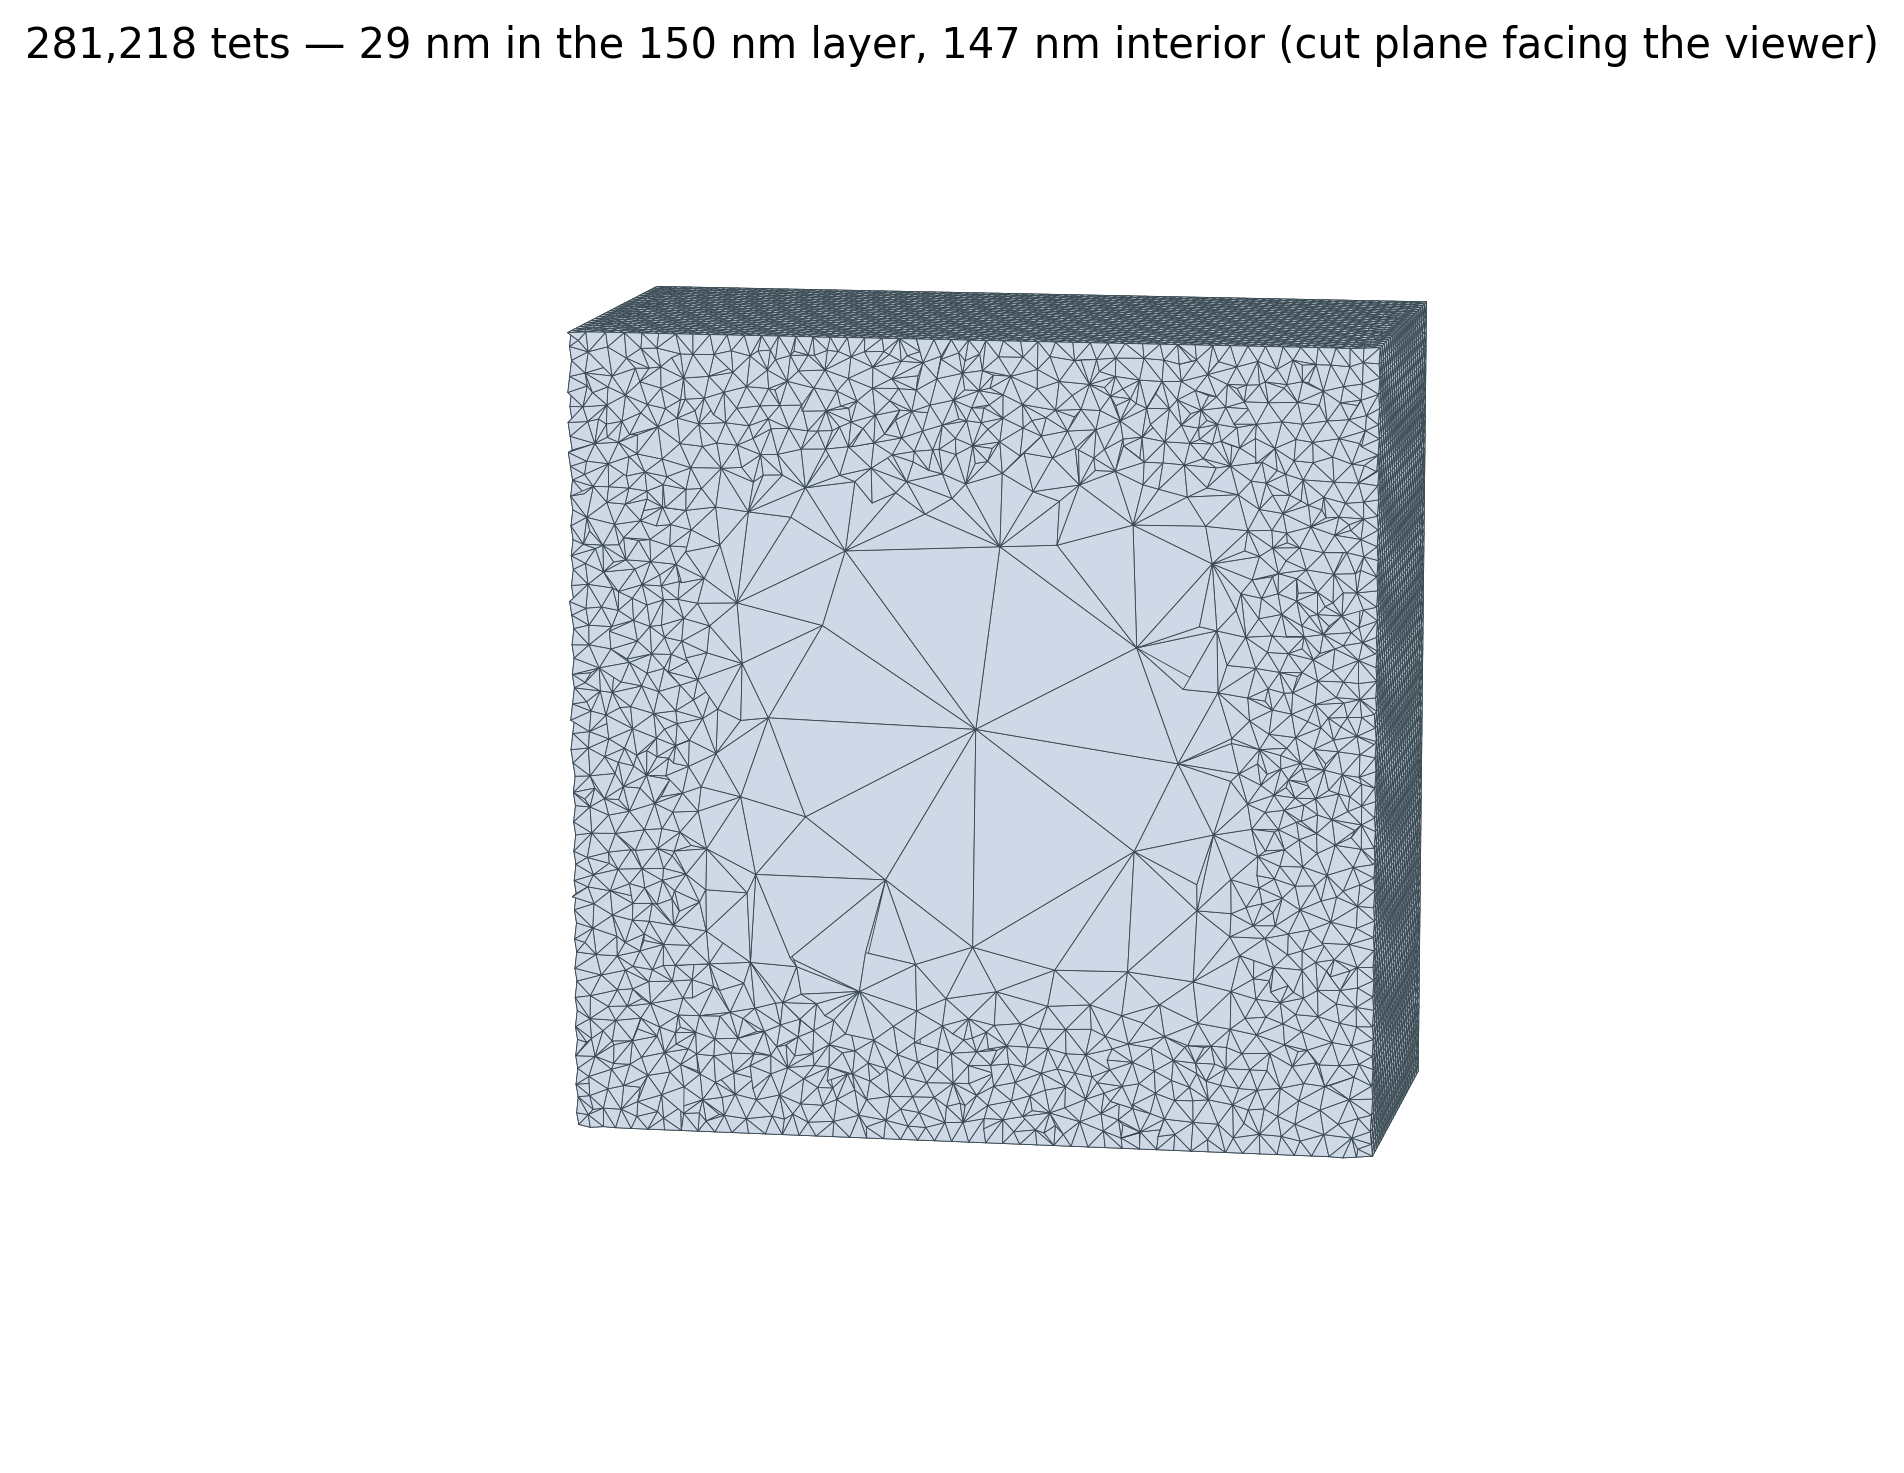
\includegraphics[width=0.48\linewidth]{figures/mesh_E_281218tets.png}
\hfill
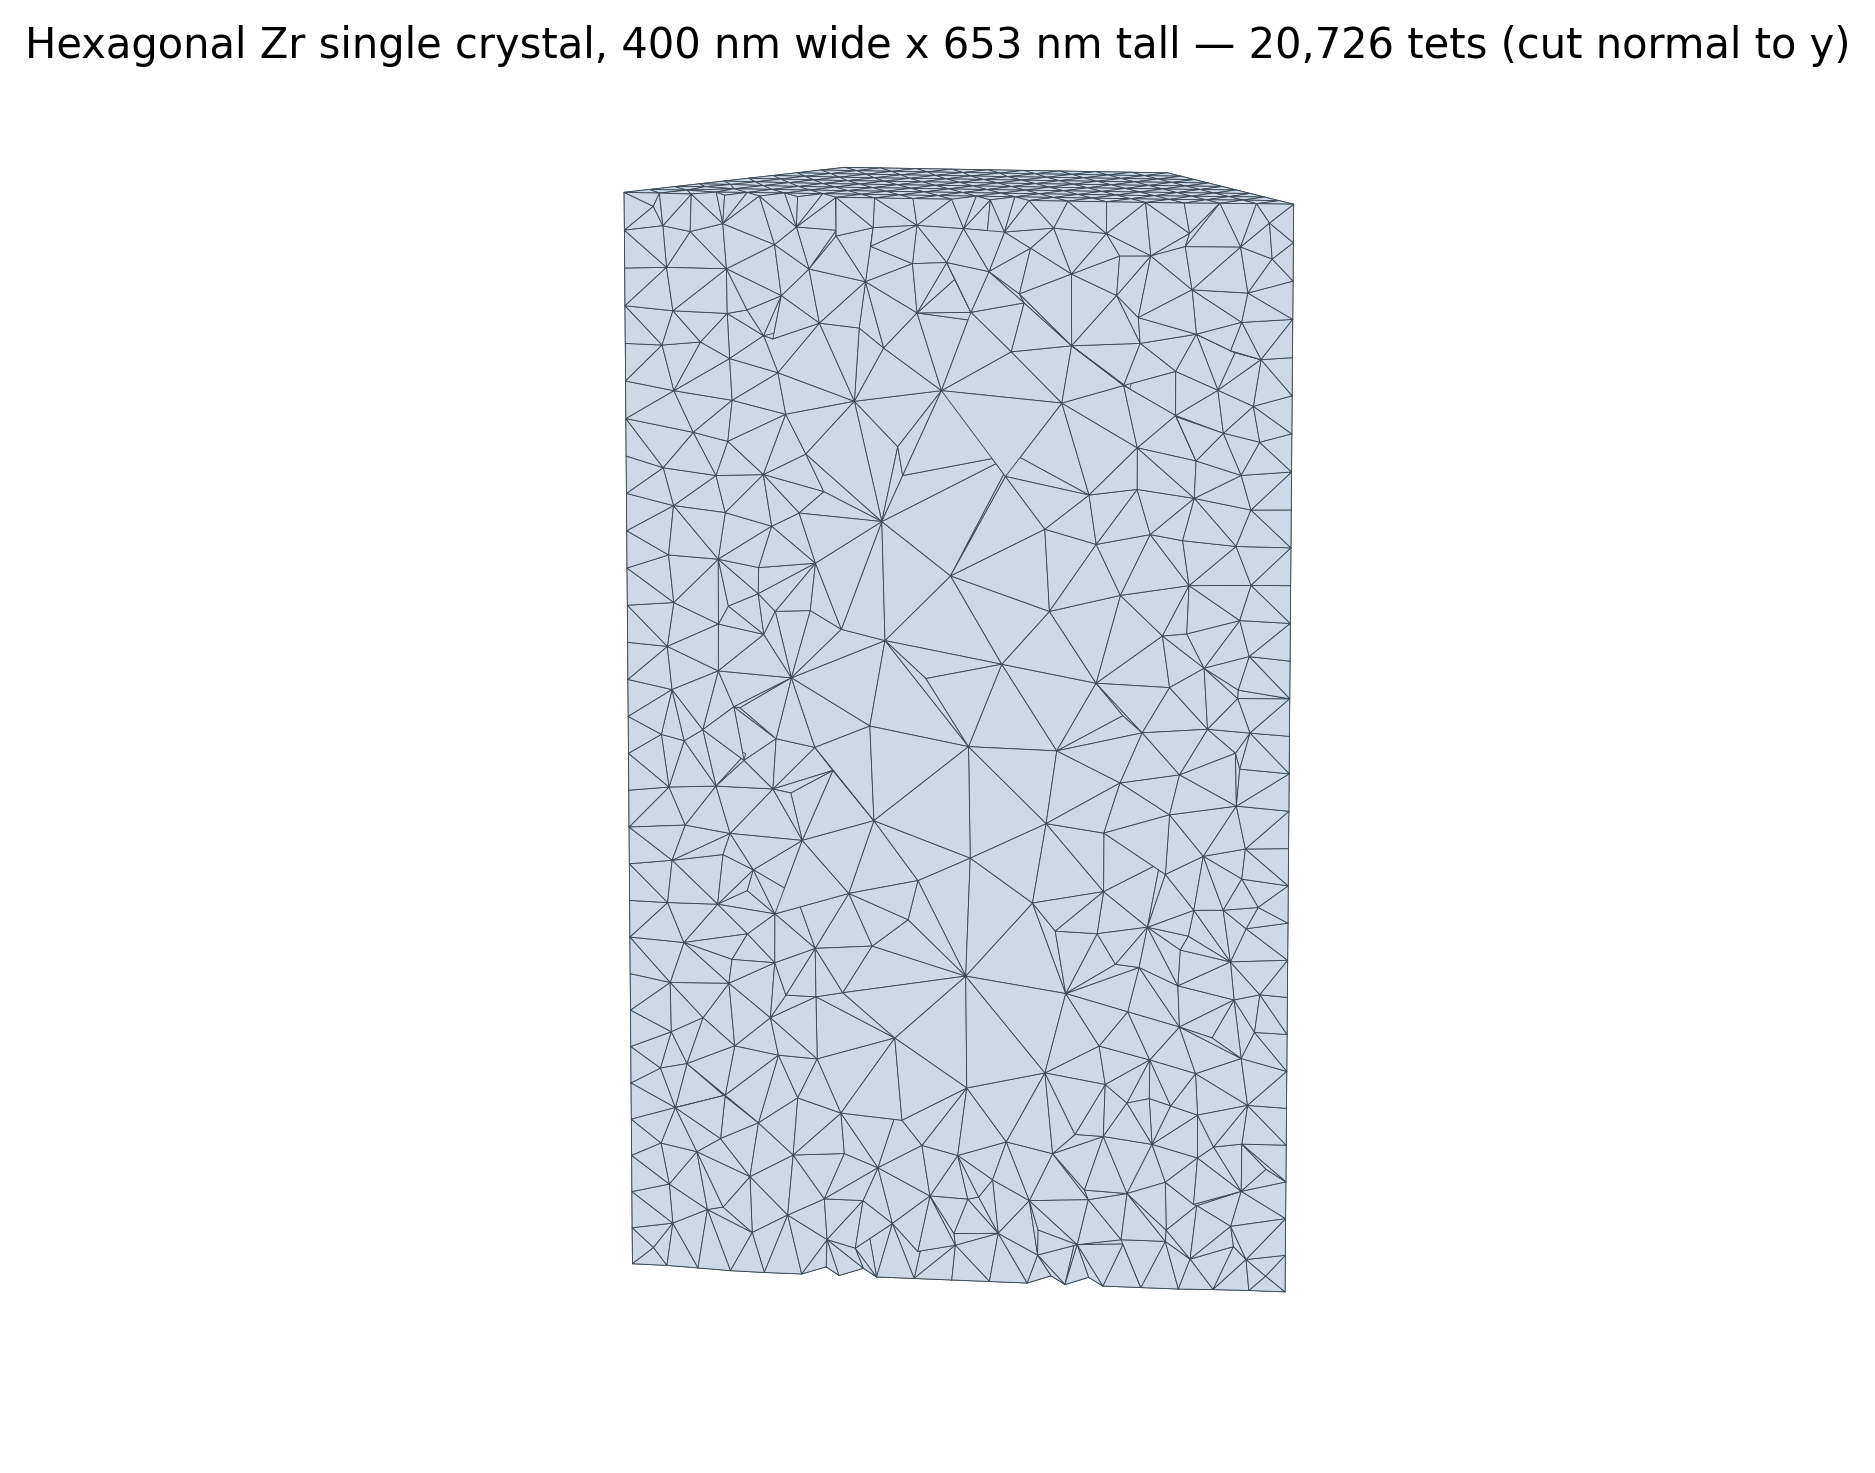
\includegraphics[width=0.48\linewidth]{figures/mesh_hex400_cut_y.png}
\caption{Mesh-dependence studies. Left: cubic verification domain, 281{,}218 tetrahedra, graded from 29~nm in the 150~nm boundary layer to 147~nm in the interior (cut plane facing the viewer). Right: hexagonal Zr single crystal, 400~nm wide by 653~nm tall, 20{,}726 tetrahedra (cut normal to $y$).}
\label{fig:mesh-dependence}
\end{figure}

\paragraph{Prismatic loop size distributions.}
Figure~\ref{fig:size-dist-a} shows the $\langle a \rangle_3$ loop size distribution at 1 and 26~dpa. Two features carry the physics. First, the distribution is essentially monodisperse at both doses, and the number-weighted mean is stationary at 3.87~nm at 1~dpa against 3.77~nm at 26~dpa, while the bin population grows by more than an order of magnitude, from about $1.3\times10^{27}$ to $3.3\times10^{28}$ loops per m$^3$. The prismatic population is therefore nucleation-dominated: cascades inject new loops at the nucleation size faster than the existing loops grow, and additional dose is stored as number density at nearly constant size. Second, the width of the histogram is spatial rather than physical. Each node carries a single mean size per family, so the plotted spread measures the variation of the local mean across the grain; the sharpness of the peak is itself a verification statement, showing that the interior is well mixed, as the reconciliation with the 0-D model requires, while the sparse large-diameter tail is contributed by the few near-boundary nodes whose local density and net flux depart from the interior values.

\begin{figure}[htbp]
\centering
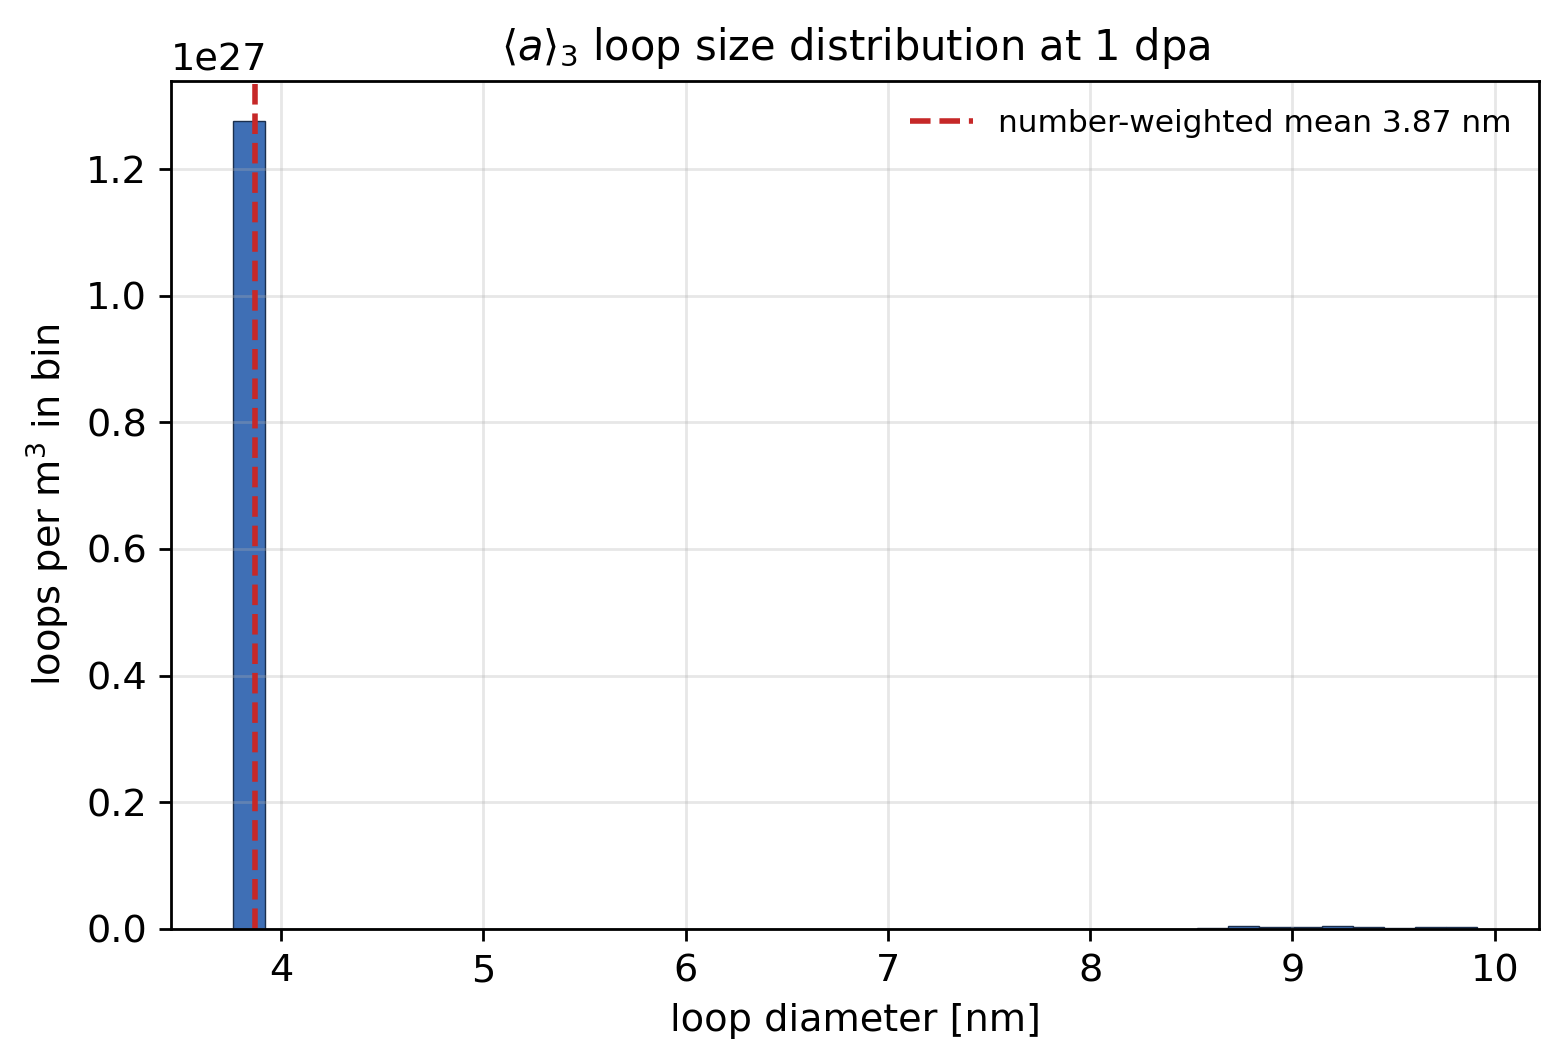
\includegraphics[width=0.48\linewidth]{figures/size_dist_a3_01dpa.png}
\hfill
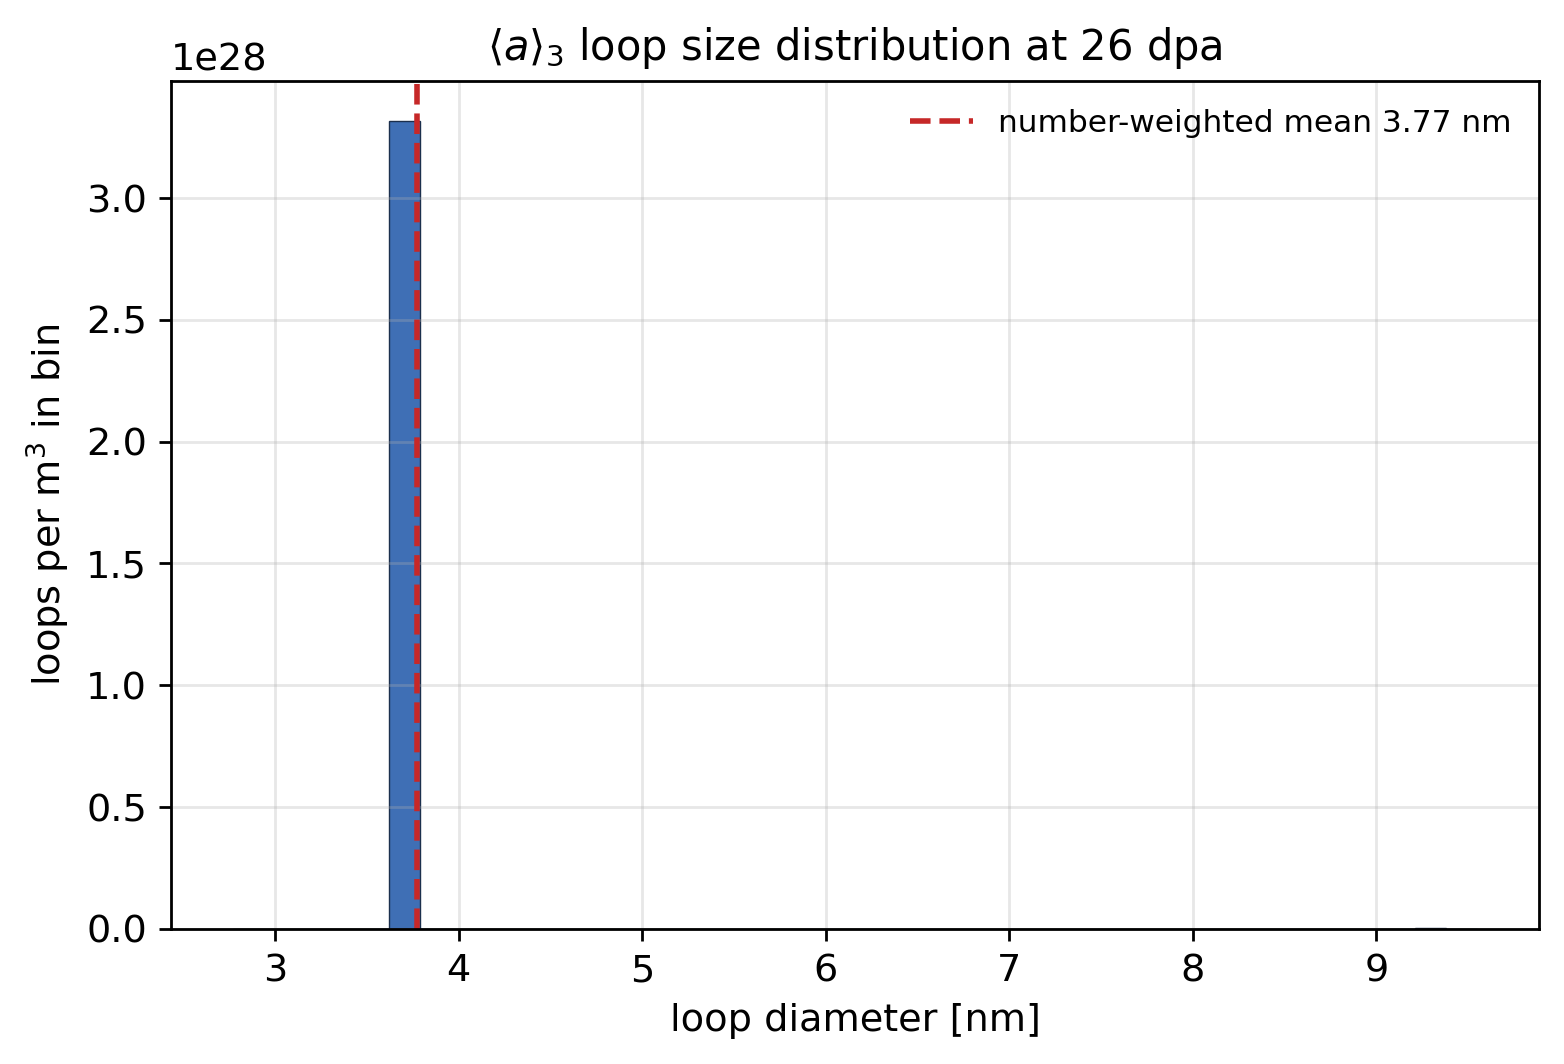
\includegraphics[width=0.48\linewidth]{figures/size_dist_a3_26dpa.png}
\caption{$\langle a \rangle_3$ loop size distributions at 1~dpa (left) and 26~dpa (right). The number-weighted mean diameter is nearly dose-independent while the number density grows by more than an order of magnitude, the signature of a nucleation-dominated population.}
\label{fig:size-dist-a}
\end{figure}

\paragraph{Basal loop size distributions.}
The $\langle c \rangle$ population of Fig.~\ref{fig:size-dist-c} responds to dose in the opposite way. The distribution is bimodal. The dominant population sits near 55~nm at 1~dpa and coarsens slowly to 58--65~nm by 26~dpa, moving the number-weighted mean from 46.0 to 48.5~nm: basal loops nucleate rarely and at a much larger size than the prismatic loops, and subsequent dose is stored as loop growth rather than as number density. The secondary population near 20~nm is stationary in both position and amplitude between the two doses, which identifies it as spatial in origin: it collects the nodes inside the near-boundary depletion zone, where the grain boundary intercepts the mobile fluxes and the local loops are held close to their nucleation size. Its dose independence is consistent with a denuded-zone width set by the depletion length, which does not evolve with dose. The broadening of the interior peak at 26~dpa reflects the accumulated radial gradient of net absorbed flux between grain center and boundary.

\begin{figure}[htbp]
\centering
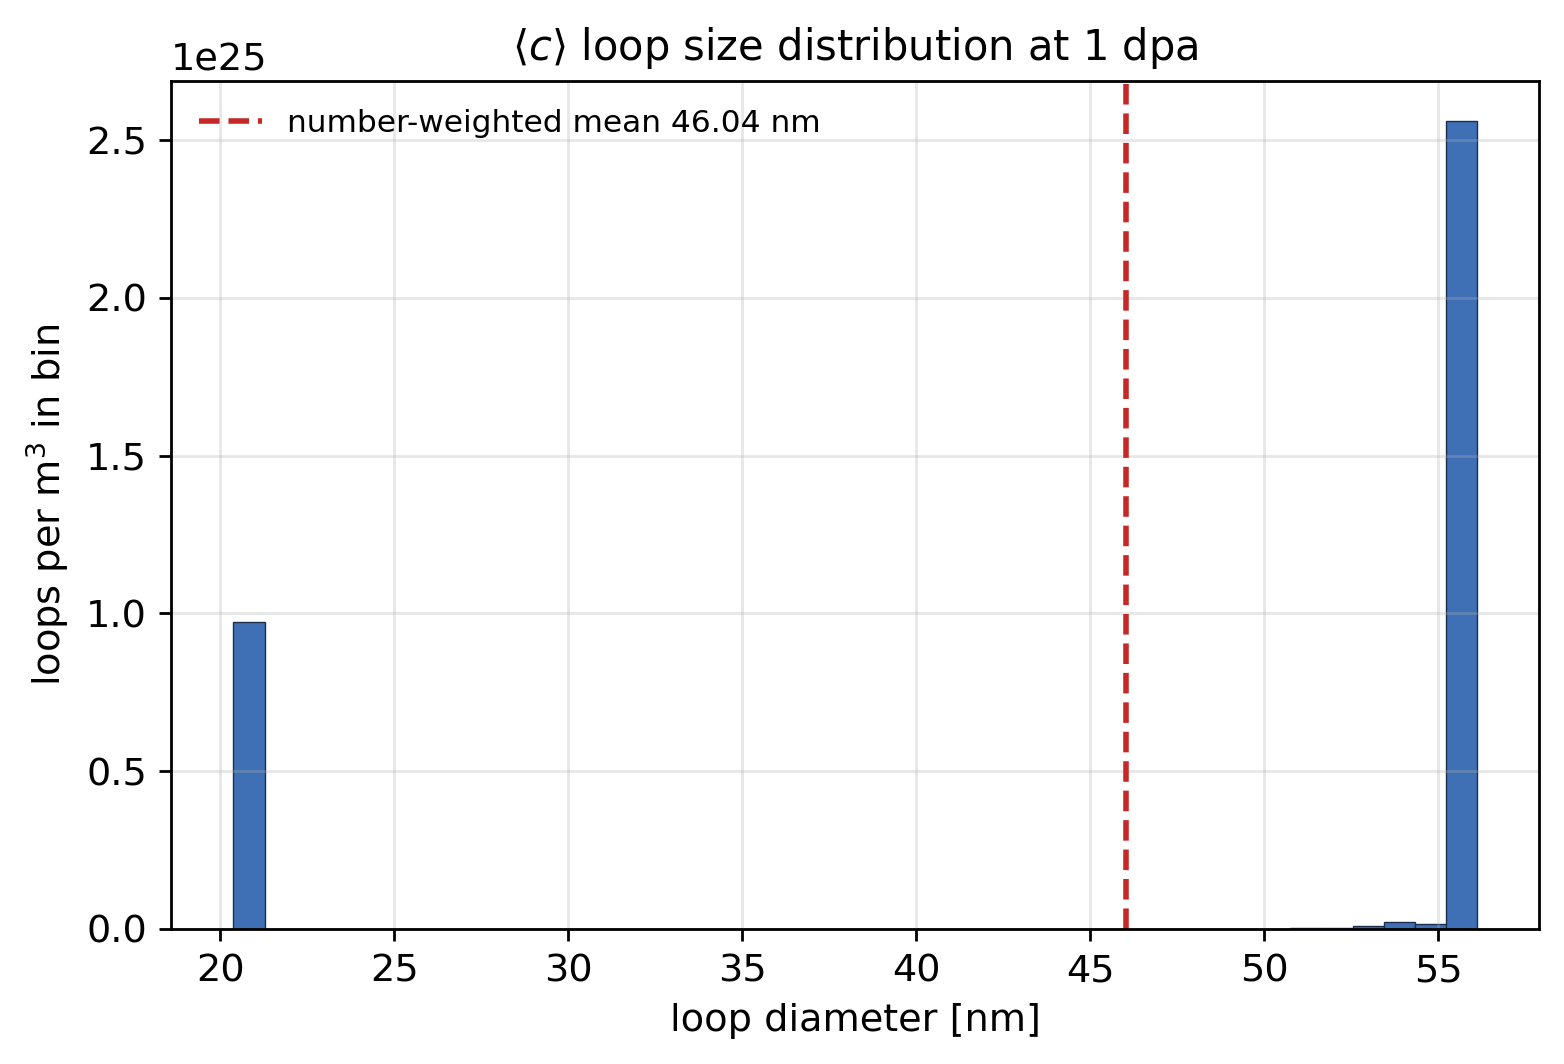
\includegraphics[width=0.48\linewidth]{figures/size_dist_c_01dpa.png}
\hfill
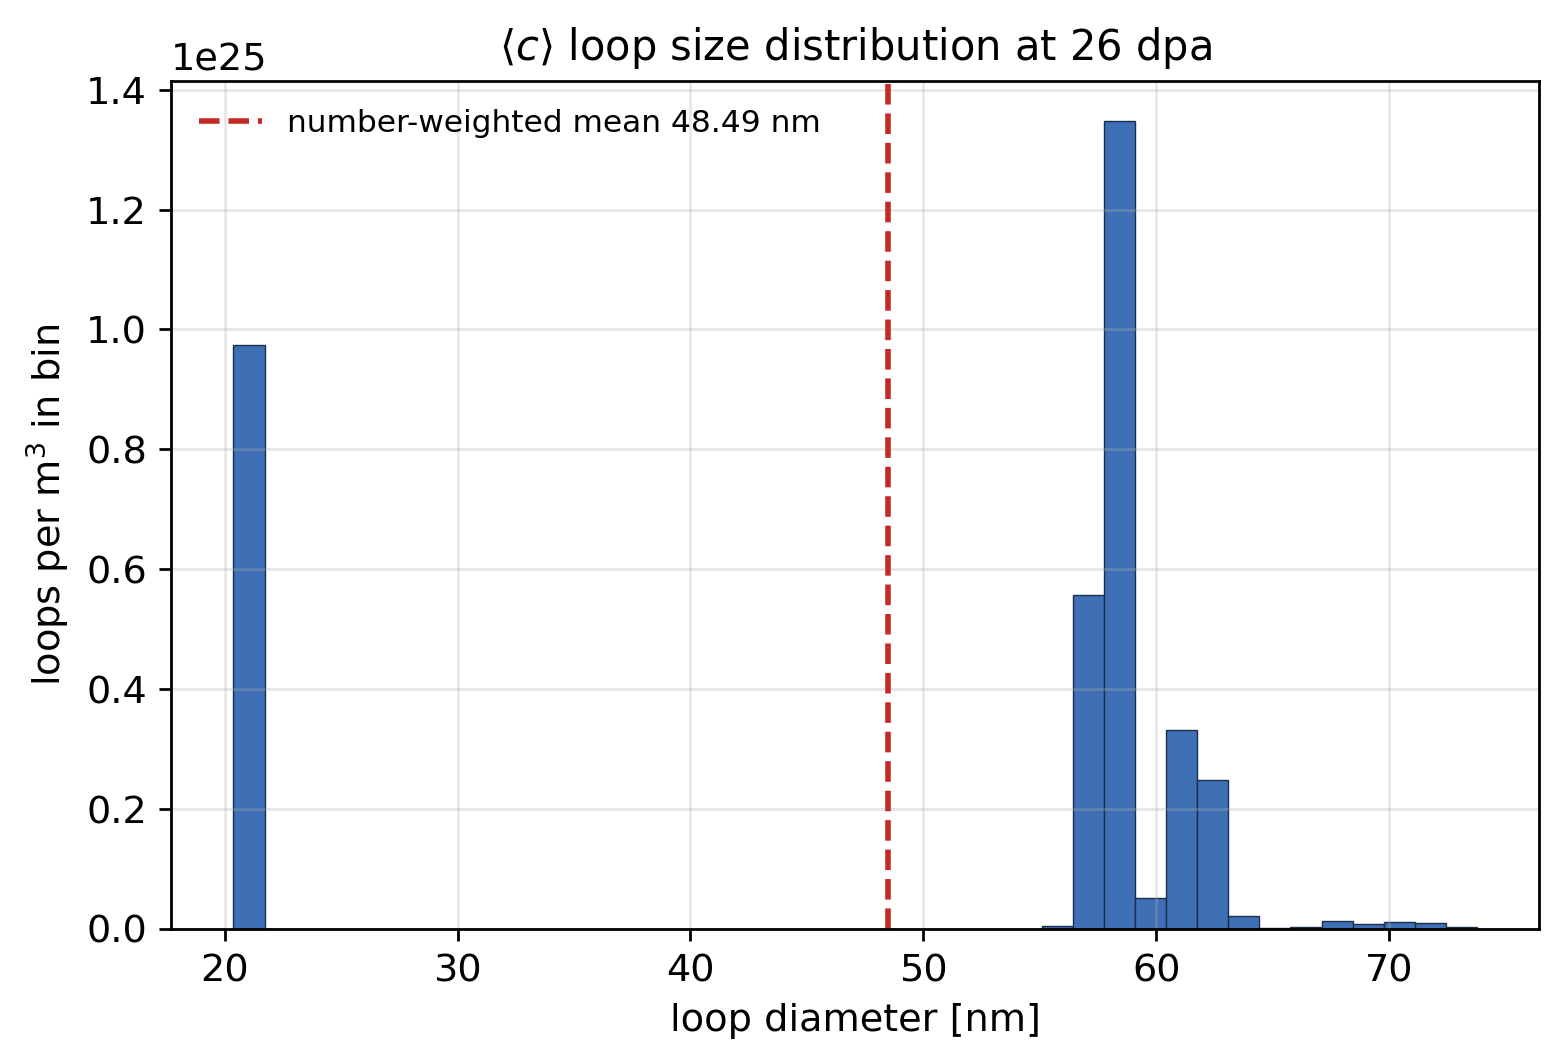
\includegraphics[width=0.48\linewidth]{figures/size_dist_c_26dpa.png}
\caption{$\langle c \rangle$ loop size distributions at 1~dpa (left) and 26~dpa (right). The interior population coarsens slowly with dose while a stationary near-boundary population remains near 20~nm; the number-weighted mean moves from 46.0 to 48.5~nm.}
\label{fig:size-dist-c}
\end{figure}

\paragraph{Loop populations in the unstressed hexagonal crystal.}
Figure~\ref{fig:loops-6dpa} renders the four loop families in the unstressed hexagonal single crystal at 6~dpa. Platelets are drawn in their habit planes with radii magnified for visibility, by a factor of 7 for the prismatic families and only 1.5 for the basal family; the basal loops are physically an order of magnitude larger. The three prismatic panels constitute the zero-stress crystallography check: with no applied stress, the three $\langle a \rangle$ Burgers-vector families are physically equivalent, and the computed $C_{\langle a \rangle 1}$, $C_{\langle a \rangle 2}$, and $C_{\langle a \rangle 3}$ fields are statistically indistinguishable, each carrying one third of the prismatic population and differing only in habit-plane orientation. Any systematic departure among the three panels would indicate an error in the crystallographic bookkeeping rather than in the physics. The cut planes make the spatial structure quantitative. The prismatic content, plotted on a logarithmic scale spanning $10^{-4}$ to $10^{-3}$, is uniform over the grain interior, with a narrow band of elevated content within the depletion layer at the boundary; the basal content, on a linear scale up to $2\times10^{-3}$, shows the same flat interior plateau but is denuded at the boundary. The opposite sign of the two near-boundary perturbations reflects the different depletion profiles of the two mobile species within the boundary layer: the net interstitial flux feeding the prismatic loops is locally enhanced where the boundary drains the vacancy field, while the basal vacancy loops lose their growth flux there. Both rims are confined to a few depletion lengths, and the uniformity of all four interior fields is the spatial statement of the reconciliation objective: away from the boundary layer the 3-D solution reduces to the well-mixed limit described by the 0-D model.

\begin{figure}[htbp]
\centering
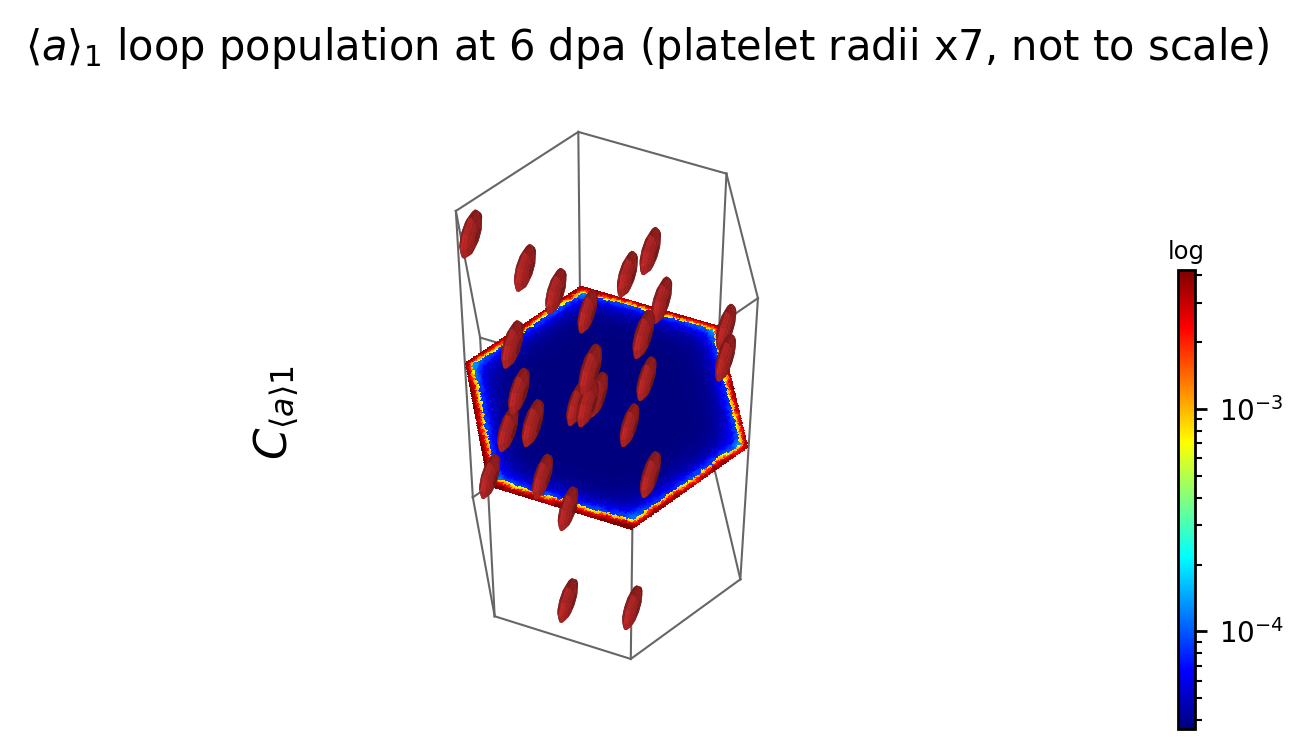
\includegraphics[width=0.48\linewidth]{figures/loops_a1_06dpa.png}
\hfill
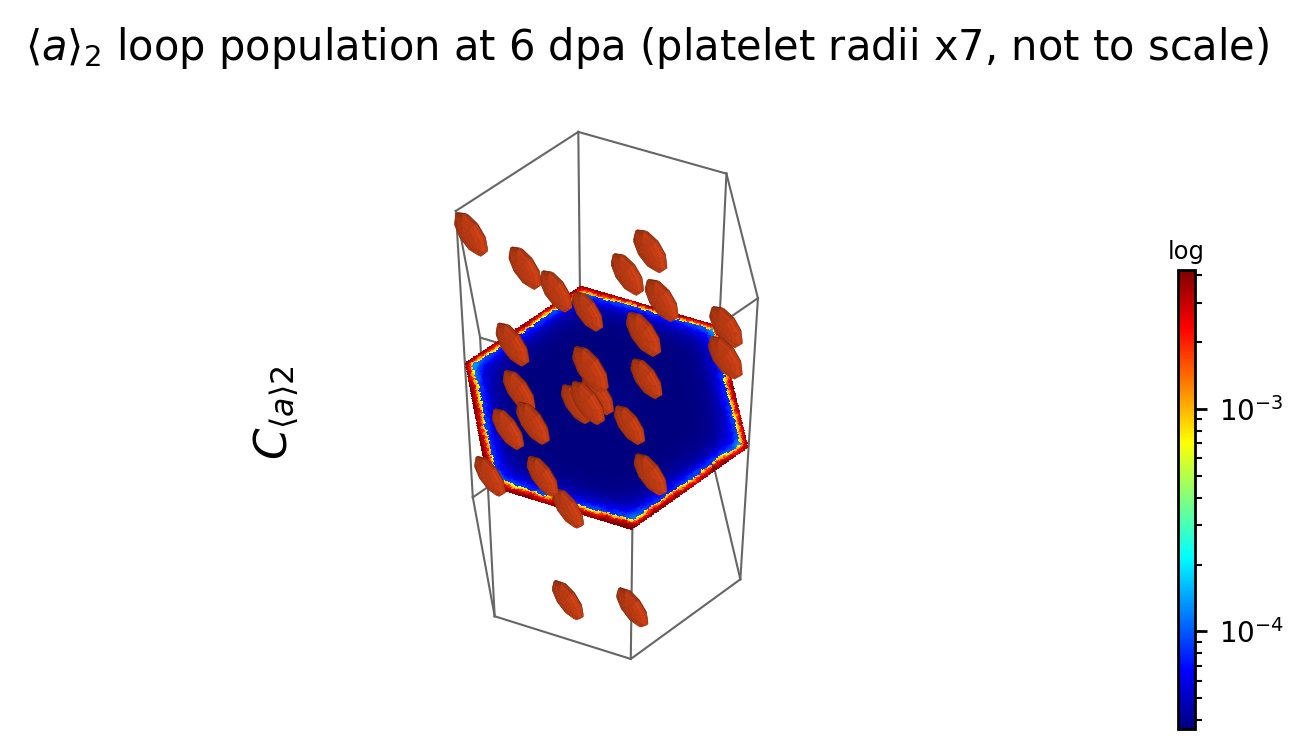
\includegraphics[width=0.48\linewidth]{figures/loops_a2_06dpa.png}\\[2pt]
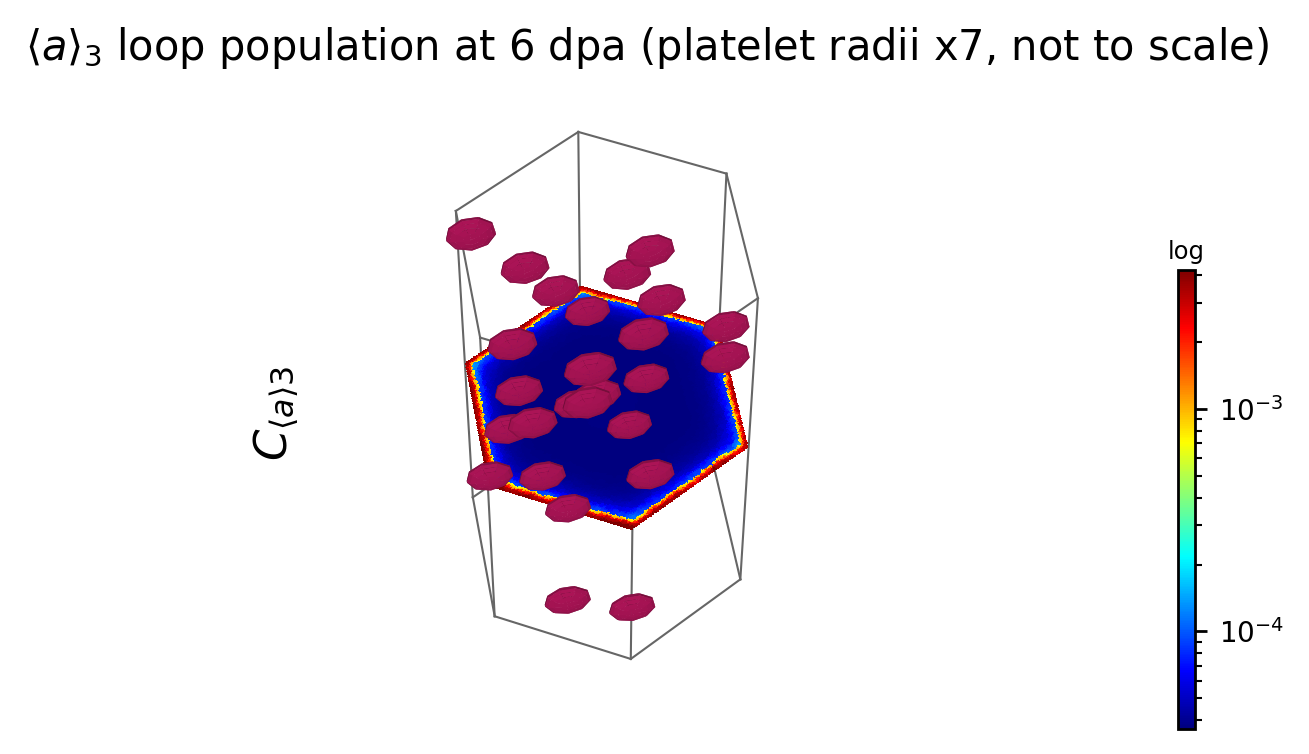
\includegraphics[width=0.48\linewidth]{figures/loops_a3_06dpa.png}
\hfill
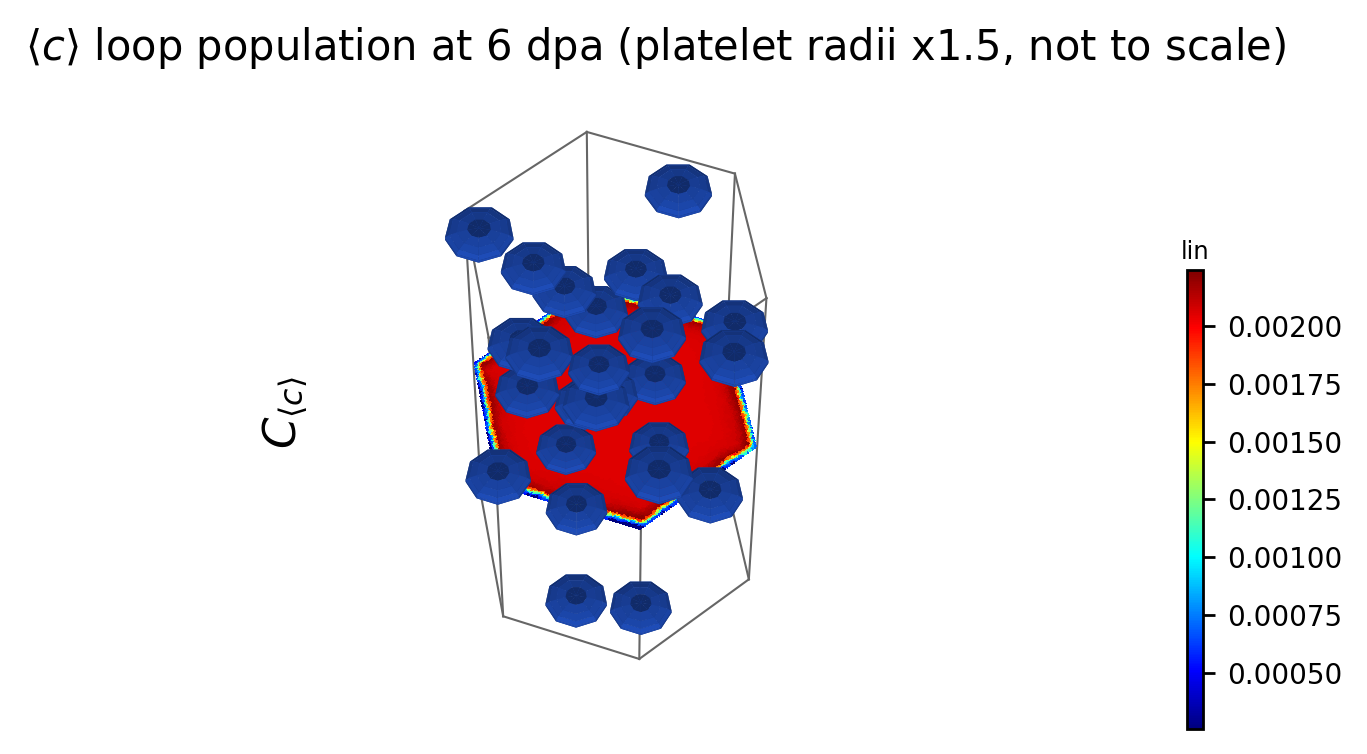
\includegraphics[width=0.48\linewidth]{figures/loops_c_06dpa.png}
\caption{Loop populations in the unstressed hexagonal single crystal at 6~dpa; platelet radii are magnified ($7\times$ prismatic, $1.5\times$ basal) and are not to scale. Top row and bottom left: the three prismatic $\langle a \rangle$ families, whose statistical equivalence at zero stress is the built-in crystallography check. Bottom right: the basal $\langle c \rangle$ family, physically much larger and denuded within the boundary depletion layer.}
\label{fig:loops-6dpa}
\end{figure}

%==============================================================================
\subsection{Summary and Outstanding Items}
\label{sec:summary}

{\ZrM} reproduces the {\ZrOd} rate coefficients to within 0.1\%
(Table~\ref{tab:reactions}) and its interior mobile-defect concentrations and
\cloop{} loop density to within a few percent, stably from 1 dpa to
30 dpa (Table~\ref{tab:verification}). The experimental calibration
embedded in {\ZrOd} therefore transfers to the three-dimensional model in the
well-mixed limit, which was the objective set out in Section~\ref{sec:intro}.

The following items remain open.

\begin{enumerate}
\item \textbf{Homogeneous nucleation.} The clustering flux
$\Phi_{\rm clus} = R_{i,3i} + R_{2i,2i}$ is not wired into the loop nucleation
term. It is exact at zero stress only in the sense that the SIPN weights are then
uniform; the channel itself is missing, and its sign is consistent with the
\aloop{} density deficit.
\item \textbf{Grain boundaries as loop sinks.} See the caution in
Section~\ref{sec:results}.
\item \textbf{Di-interstitial consumption.} The dose dependence of the $C_{2i}$
ratio in Table~\ref{tab:verification} is not understood.
\item \textbf{The DAD is a fitting form, not a generated one.} The parameters
$p_m$ and $Z^0_m$ in Eq.~\eqref{eq:dad} are fitted to reproduce the 0-D symmetric
bias forms rather than derived from the ratio of diffusivities, and the diffusion
tensors have been made isotropic to match \ZrM{}. The present calculations
, therefore, do not exercise the tensorial DAD mechanism, and the fit is tied to
573~K.
\item \textbf{Upstream defect.} The binding energy initialization-order bug
described in Section~\ref{sec:changes} affects any \MoD{} calculation with a
non-negligible cluster binding energy and should be reported.
\end{enumerate}



%%%%%%%%%%%%%%%%%%%%%
\section{Conclusions}

This deliverable has established and exercised two complementary realizations of the same cluster-dynamics physics for irradiation damage in zirconium: {\ZrOd}, a reduced, spatially averaged (0D) model equipped with a systematic procedure for identifying its parameters from a temperature- and dose-resolved experimental database, and {\ZrM}, a three-dimensional, spatially resolved implementation of the identical reaction network built on the {\MoD} finite-element framework. Both models integrate the coupled rate equations for the mobile point defects and the four loop families---interstitial and vacancy loops, each split into randomly oriented and DAD-aligned subsets---and return the full microstructural trajectory from the onset of irradiation through saturation. Calibrated against measured loop densities and diameters across the relevant temperature range, the reduced model reproduces the principal features of the irradiated microstructure at a computational cost low enough to make large parameter sweeps and inverse identification practical, while the spatial model carries the calibrated kinetics into finite grains with absorbing boundaries and resolves the intra-granular structure that the mean-field description necessarily averages away. The results below summarize the physical conclusions drawn from the two sets of simulations, from their reconciliation, and from the comparison with the Zr database, together with the lessons learned in the course of building, calibrating, and cross-verifying the codes.

\begin{enumerate}
\item \textbf{Defect kinetics follow a build-up, overshoot, and saturation sequence.} The free vacancy concentration rises and saturates first, with free interstitials sitting well below it; the di- and tri-interstitial channels remain negligible. The total stored-defect curve exhibits an early build-up, a mild overshoot near a fraction of a dpa, and a saturation plateau that is inherited by all downstream microstructural quantities.
\item \textbf{A small, sign-definite vacancy–interstitial imbalance is the microscopic driver of growth.} The orientation bias produces a saturating net flux to the sinks whose sign is fixed; this imbalance, rather than the absolute fluxes (which rise and saturate together), is what couples the defect kinetics to the macroscopic growth strain.
\item \textbf{Loop densities and a-loop sizes are well reproduced.} Both loop families nucleate within a narrow dose window, pass through a modest overshoot, and saturate. The interstitial (a) loop diameter saturates in agreement with the low-to-mid temperature data, and the temperature-resolved a-loop densities track the measured thermal suppression of the saturation level with increasing temperature.
\item \textbf{The main residual discrepancy is the c-loop (vacancy) diameter.} The vacancy-loop diameter saturates below the measured value, while its number density matches the reference data and brackets the available measurements. This is the principal quantitative gap between model and experiment and points to missing physics in the vacancy-loop coarsening channel.
\item \textbf{Interstitial loops control number density; vacancy loops control stored volume.} The decomposition of the saturated population by family and orientation shows a clear division of roles, which clarifies how each population contributes to the macroscopic observables. The {\ZrM} size distributions expose the mechanism behind this division: the prismatic population is nucleation-dominated---essentially monodisperse near 4~nm while its number density grows by more than an order of magnitude, so additional dose is stored as new loops at nearly constant size---whereas the basal population is growth-dominated, nucleating rarely and at much larger size, saturating its number density almost immediately at the balance between cascade nucleation and embryo dissolution, and storing subsequent dose as coarsening of the surviving loops.
\item \textbf{The network and sink geometry evolve consistently.} The network dislocation density relaxes from its grown-in seed and saturates as unfaulted loops feed the network, and coalescence limits further growth; the loop-to-network and loop-to-loop spacings contract as the loop density builds and saturates at the inter-obstacle distance that governs hardening and coalescence.
\item \textbf{The spatial model reproduces the mean-field kinetics in the well-mixed limit.} {\ZrM} matches the {\ZrOd} rate coefficients to within 0.1\% and reproduces the interior mobile-defect concentrations and the \cloop{} loop density to within a few percent, stably from 1 to 30~dpa. The experimental calibration embedded in {\ZrOd} therefore transfers directly to the three-dimensional model: away from the grain-boundary layer, the 3D solution reduces to the well-mixed limit described by the 0D model, which was the central objective of the reconciliation of the two codes.
\item \textbf{Grain boundaries organize the microstructure into a denuded zone, and the two loop types respond in opposite senses.} The mobile fields form an interior plateau that falls to the thermal equilibrium concentration at the absorbing boundary over a depletion length small compared with the grain size, and the depleted layer thickens with dose as the loop sink strength builds. Adjacent to the boundary there are many small loops and in the interior fewer large ones; for the \aloop{} families the density excess dominates and the stored content is enhanced at the boundary, while for the \cloop{} family the size deficit is unopposed and the stored content is depleted there. Since the stored content is what enters the growth strain, this distinction carries directly into spatially resolved predictions of irradiation growth near grain boundaries.
\item \textbf{The integrations are numerically trustworthy, and cross-verification proved to be a sensitive diagnostic in its own right.} In {\ZrOd}, the conservation diagnostics keep the running relative error in the global defect balance small throughout, confirming that the production, recombination, and absorption channels are book-kept self-consistently and that the reported trends are physical rather than numerical artifacts. In {\ZrM}, every code-to-code verification ratio is constant from about 5~dpa onward---an error in a unit conversion or a rate constant would be integrated by the loop populations and appear as a drift---and the required equality of the three prismatic families at zero stress proved sensitive enough to expose a Burgers-vector bookkeeping error, as well as an upstream binding-energy initialization defect in {\MoD} itself.
\item \textbf{The remaining code-to-code residuals are structural, localized, and diagnosed.} The \aloop{} loop density in {\ZrM} sits at about half the 0D value, consistent in sign with the homogeneous clustering flux that is not yet wired into the loop-nucleation term, and the di-interstitial concentration ratio falls with dose, pointing to the cluster weighting in the loop-absorption term. Because grain boundaries are not yet sinks for the loops that grow into them, the near-boundary \aloop{} density rises without bound and should not be used quantitatively. The present spatial calculations are, in addition, restricted to zero applied stress with isotropic diffusion and a DAD bias fitted to the 0D forms at 573~K, so the tensorial DAD mechanism remains to be exercised.
\item \textbf{Lesson learned: identifiability must be managed explicitly.} The inverse problem is well posed only after the parameters are transformed and normalized onto a common scale, and only a minimal, identifiable subset is genuinely constrained by the data; the remaining parameters are best fixed at physically motivated values rather than fitted.
\item \textbf{Lesson learned: a hybrid optimization strategy is essential.} Global differential evolution, surrogate-assisted (RBF) ``self-learning'' search, and local Nelder–Mead refinement are complementary; relying on any one alone either misses the global basin or wastes expensive forward evaluations.
\end{enumerate}

Overall, the two-tier framework is a clear success for its intended purpose. With a modest, physically interpretable parameter set, the reduced {\ZrOd} model captures the dose- and temperature-dependence of the loop microstructure and the defect kinetics that drive irradiation growth, and it does so cheaply enough to support calibration and uncertainty studies. The reconciliation exercise has demonstrated that this calibration is not confined to the mean-field description: embedded in {\ZrM}, the same cluster-dynamics physics, solved by the finite-element method over resolved grains~\citep{spatialCD2024}, inherits the identified parameters in the well-mixed interior while adding what the 0D model cannot represent---the reaction--diffusion transport to absorbing grain boundaries, the denuded-zone structure of the mobile and loop fields, and the opposing near-boundary responses of the prismatic and basal populations that will shape grain-size-dependent growth.

The most promising avenues for improvement follow directly from the residual discrepancies identified above. On the mean-field side, a more faithful treatment of the vacancy-cluster-to-vacancy-loop transition and of c-loop coarsening would close the remaining gap in the c-loop diameter, together with a refined description of loop coalescence and the orientation-dependent bias factors. On the spatial side, the immediate priorities are wiring the homogeneous clustering flux into the loop-nucleation term, endowing grain boundaries with a sink for the loops that grow into them, and activating the anisotropic diffusion tensors and stress-informed bias factors beyond the present zero-stress fit at 573~K. With these elements in place, the division of labor established here---{\ZrOd} as the calibrated, locally evaluated kinetics engine and {\ZrM} as the spatial solver coupled to crystal plasticity---turns the identified parameter set into the constitutive input for full-field simulations of irradiation growth, creep, and hardening in single-crystal and polycrystalline samples, providing a direct and physically consistent bridge from the reduced kinetics to predictions of microstructure and deformation.

%%%%%%%%%%%%%
\newpage
\bibliographystyle{elsarticle-num}
\bibliography{Biblio/NNL_Zr_Refs}
\end{document}
